\documentclass[a4paper, 11pt, oneside, polutonikogreek, french]{article}
\usepackage[T1]{fontenc}
\usepackage{aurical}

% Load encoding definitions (after font package)

\usepackage{textalpha}

\usepackage{listings}
\lstset{basicstyle=\ttfamily}

% Babel package:
\usepackage[french]{babel}

% With XeTeX$\$LuaTeX, load fontspec after babel to use Unicode
% fonts for Latin script and LGR for Greek:
\ifdefined\luatexversion \usepackage{fontspec}\fi
\ifdefined\XeTeXrevision \usepackage{fontspec}\fi

% "Lipsiakos" italic font `cbleipzig`:
\newcommand*{\lishape}{\fontencoding{LGR}\fontfamily{cmr}%
		       \fontshape{li}\selectfont}
\DeclareTextFontCommand{\textli}{\lishape}

\usepackage[dvipsnames]{xcolor}
\usepackage{eso-pic,graphicx}
\usepackage[top=70mm, bottom=45mm, outer=29mm, inner=29mm]{geometry}
\setlength{\columnsep}{90pt}

\usepackage{setspace}
\onehalfspacing

\usepackage{booktabs}
\setlength{\emergencystretch}{15pt}
\usepackage{fancyhdr}
\usepackage{microtype}
\usepackage[titles]{tocloft}
\usepackage{sectsty}

\allsectionsfont{\bfseries\Fontauri}
\sectionfont{\bfseries\Fontauri\Huge}
\subsectionfont{\bfseries\Fontauri\LARGE}
\subsubsectionfont{\bfseries\Fontauri\LARGE}
\paragraphfont{\bfseries\Fontauri\LARGE}

% change color of text, example replace all \color{Goldenrod} with \color{lightgray}
\definecolor{customColor}{RGB}{102, 2, 60}

\makeatletter % change only the display of \thepage, but not \thepage itself:
\patchcmd{\ps@plain}{\thepage}{\bfseries\large\color{customColor}{\thepage}}{}{}
\makeatother

\color{customColor}

\begin{document}
\Fontauri
\bfseries
\pagestyle{plain} % after changing a pagestyle command, it's necessary to invoke it explicitly

\renewcommand\thefootnote{\bfseries\Fontauri{\tiny\arabic{footnote}}}
\let\oldfootnote\footnote
    \renewcommand{\footnote}[1]{\oldfootnote{\bfseries\Fontauri\large#1}}

\AddToShipoutPictureBG{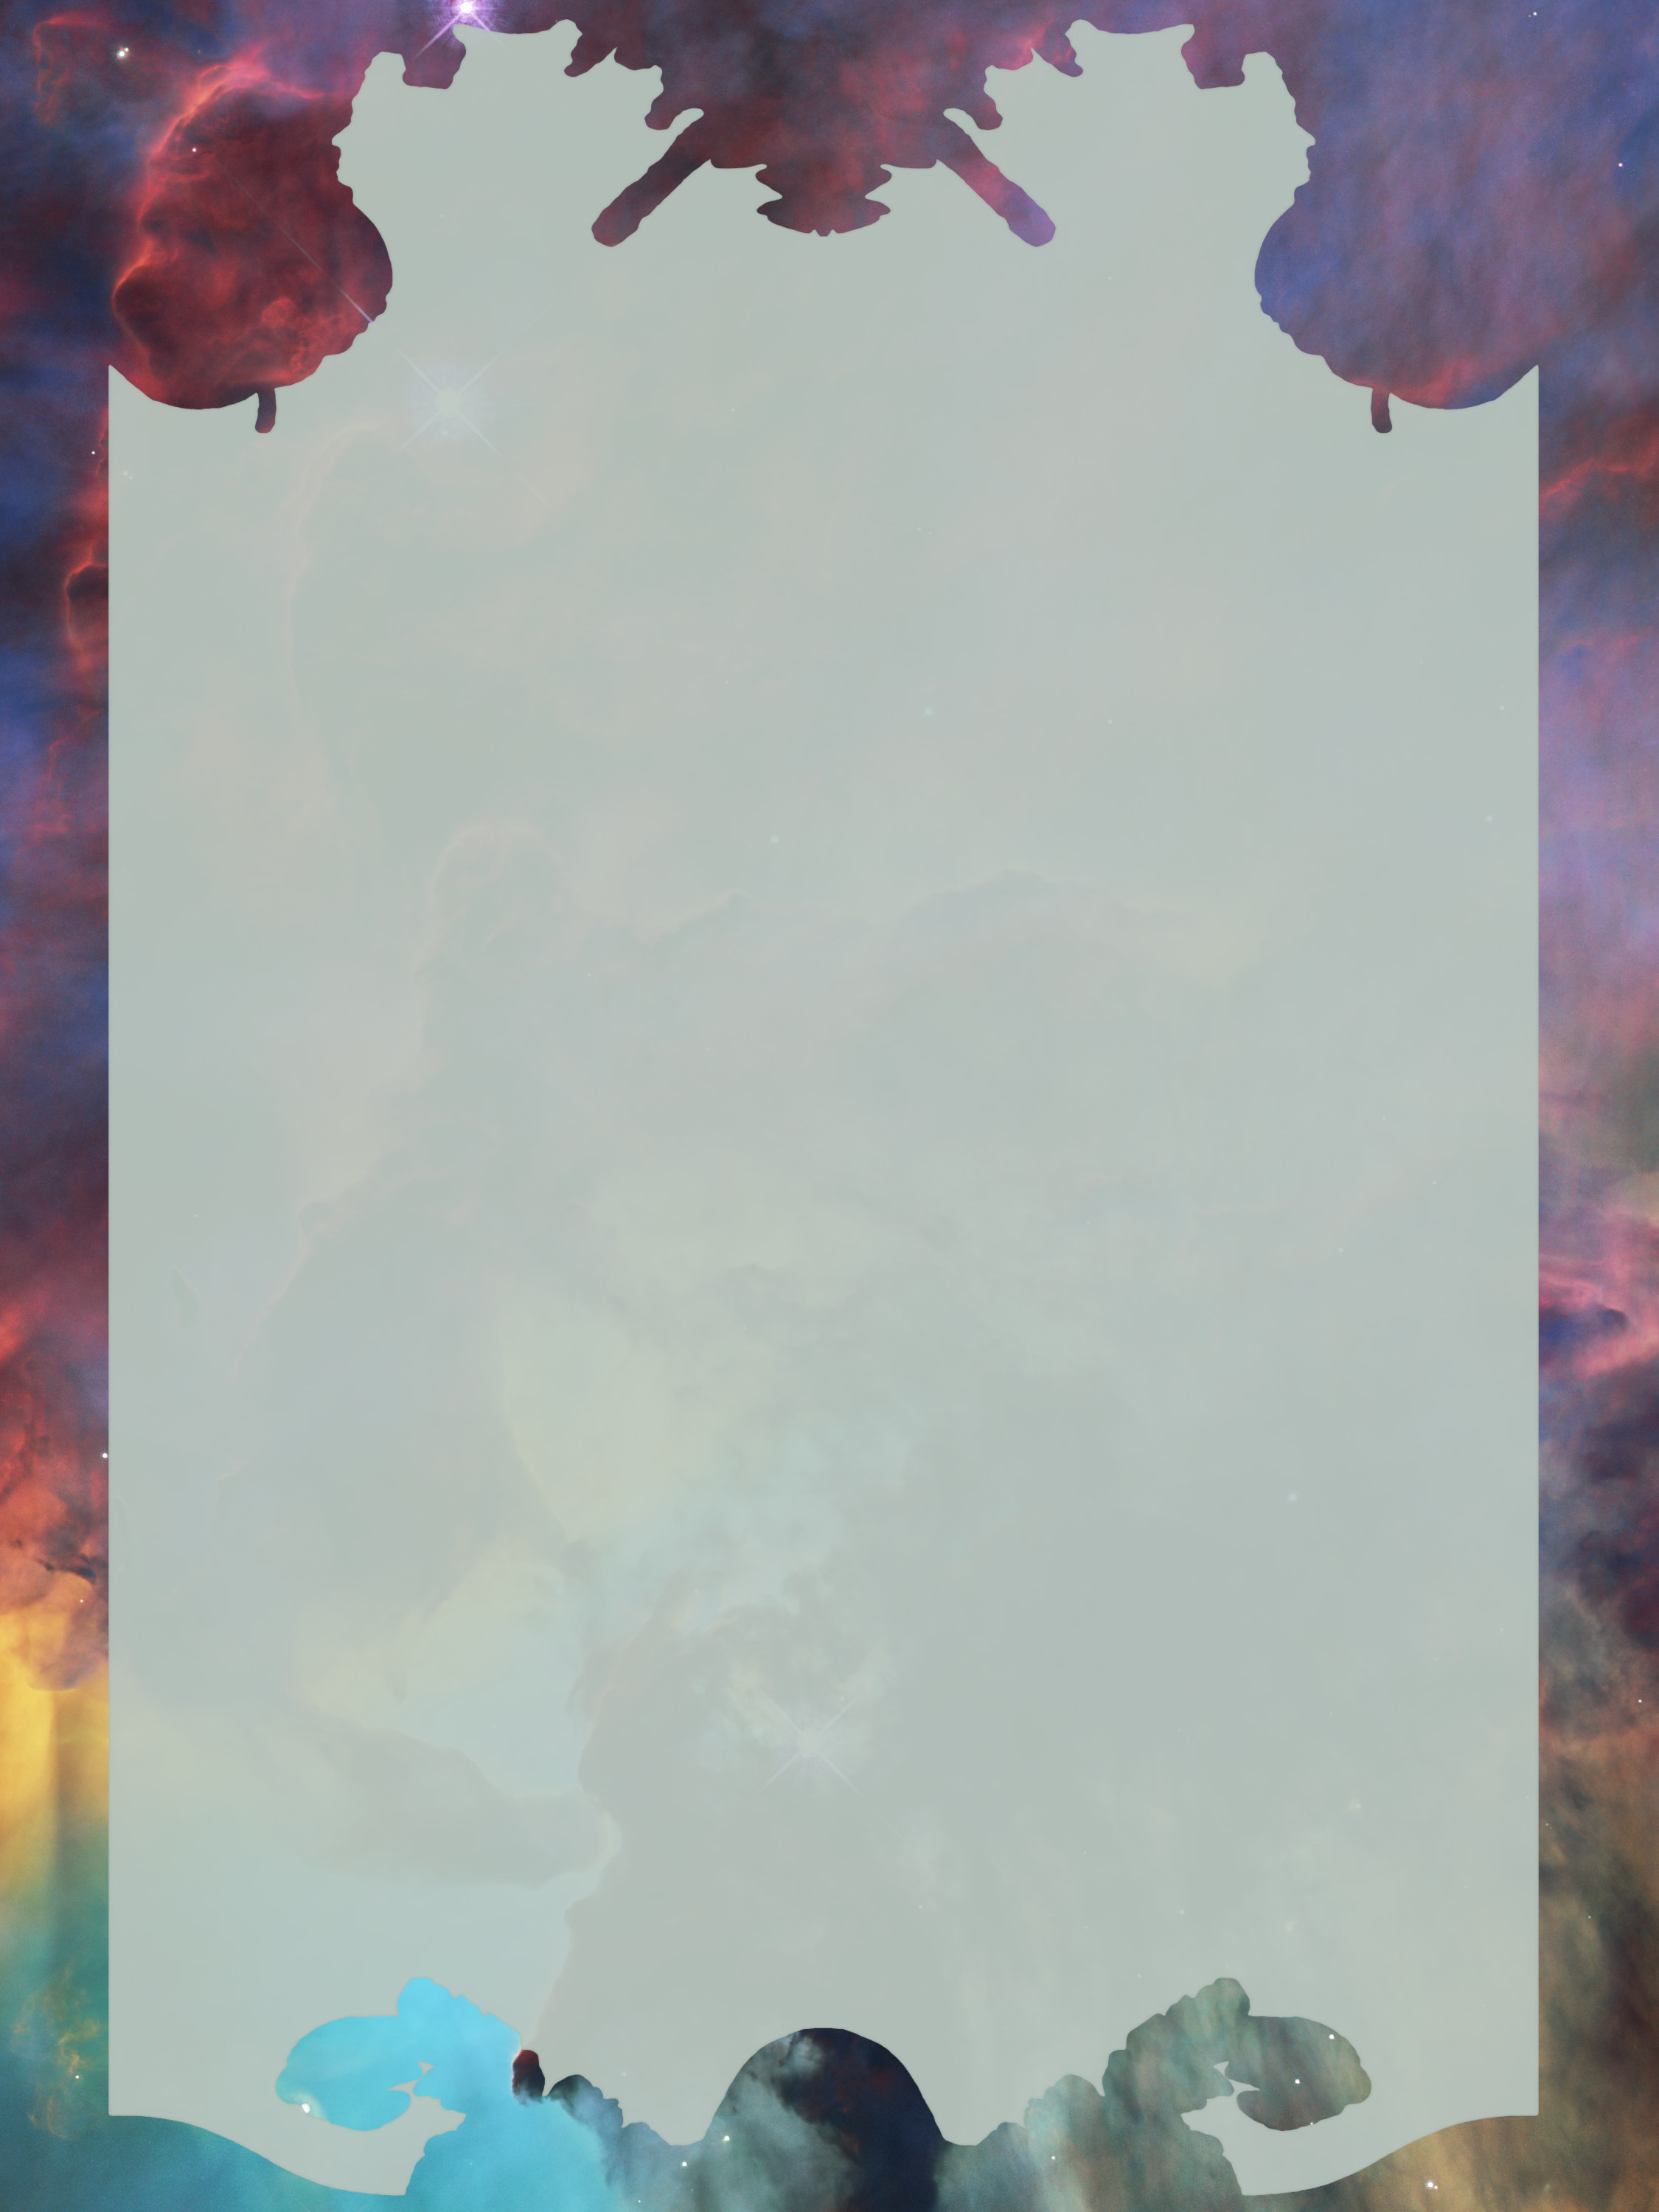
\includegraphics[width=\paperwidth,height=\paperheight]{hubble.jpeg}}


\renewcommand{\contentsname}{
\Fontauri{Table des matières}
}
\begin{titlepage} % Suppresses headers and footers on the title page
	\centering % Centre everything on the title page
	%\scshape % Use small caps for all text on the title page

	%------------------------------------------------
	%	Title
	%------------------------------------------------
	
	\rule{\textwidth}{1.6pt}\vspace*{-\baselineskip}\vspace*{2pt} % Thick horizontal rule
	\rule{\textwidth}{0.4pt} % Thin horizontal rule
	
	\vspace{1\baselineskip} % Whitespace above the title
	
	{\scshape\Huge Des Pierres Tombées du Ciel,\\ ou\\ Lithologie Atmosphérique.}
	
	\vspace{1\baselineskip} % Whitespace above the title

	\rule{\textwidth}{0.4pt}\vspace*{-\baselineskip}\vspace{3.2pt} % Thin horizontal rule
	\rule{\textwidth}{1.6pt} % Thick horizontal rule
	
	\vspace{1\baselineskip} % Whitespace after the title block
	
	%------------------------------------------------
	%	Subtitle
	%------------------------------------------------
	
	{\scshape \Large Présentant la Marche et l'Etat actuel de la Science, sur le Phénomène des \emph{Pierres de foudre}, \emph{Pluies de pierres}, \emph{Pierres tombées du ciel}, \emph{etc.} ; plusieurs Observations inédites, communiquées par MM. Pictet, Sage, Darcet et Vauquelin ; avec un Essai de Théorie sur la formation de ces \emph{Pierres}.} % Subtitle or further description
	
	\vspace*{1\baselineskip} % Whitespace under the subtitle
	
        {\scshape Par Joseph Izarn, Médecin, Professeur de Physique ; de la Société des Sciences, Belles-Lettres et Arts de Paris ; Secrétaire de la Commission d'Expériences de la Société Galvanique, et Correspondant de plusieurs Sociétés savantes. } % Subtitle or further description
    
	%------------------------------------------------
	%	Editor(s)
	%------------------------------------------------
        \vspace*{\fill}

	\vspace{1\baselineskip}

	{\small\scshape Paris 11 Avril 1803.}
	
	{\small\scshape{Chez Delalain Fils, Libraire, quai des Augustins, n°. 38, au coin de la rue Pavée.}}
	
	\vspace{0.5\baselineskip} % Whitespace after the title block

        \scshape Internet Archive Online Edition  % Publication year
	
	{\scshape\small Utilisation non commerciale --- Partage dans les mêmes conditions 4.0 International} % Publisher
\end{titlepage}
\setlength{\parskip}{1mm plus1mm minus1mm}
\clearpage
\Large
\pagestyle{fancy}
\fancyhf{}
\cfoot{\Fontauri{\thepage}}
\vspace*{\fill}
\begin{center}
{\Large \emph{De hoc multi multa, omnes aliquid},}

\textbf{Nemo Satis}.

(Inscript. de la Pierre d'Ensishem.)
\end{center}
\vspace*{\fill}
\clearpage
\tableofcontents
\clearpage
\subsection*{\Fontauri{Au Citoyen Laplace, Membre du Sénat Conservateur, de l'Institut National de France, \emph{etc.}, \emph{etc.}}}
\paragraph{}
Citoyen Sénateur,

Le phénomène sur lequel les travaux de MM. Howard et Vauquelin ont fixé l'attention générale, touchait de trop près aux régions dont vous avez su faire votre domaine, pour ne pas exciter en vous un intérêt particulier. Pouvez-vous ne pas sourire à l'idée d'une correspondance immédiate entre ces masses, qui sont l'objet principal de vos profondes méditations, et celle qui vous compte parmi ses habitants dont elle s'honore le plus ?

Vous avez manifesté le désir de voir constater la réalité du phénomène.\footnote{\Fontauri{Dans la Séance de la première Classe de l'Institut National, après la lecture du Mémoire de M. Vauquelin, le 10 frimaire an 11. 5. p. 345. (\emph{Note de l'éditeur.})}} Les recherches que j'ai faites d'abord pour mon instruction, m'ont offert des résultats que j'ai cru propres à remplir vos vues. Vous avez bien voulu prendre connaissance de mon travail, et vous l'avez jugé digne de l'attention des Physiciens, puisque vous avez permis qu'il leur fût présenté sous les auspices de l'illustre auteur de \textbf{La Méchanique Céleste}.

Une telle faveur donnerait de moi une idée trop avantageuse, et je jouirais d'une gloire usurpée, si je ne publiais que la première idée de cet Ouvrage vous appartient, et que, s'il a quelque mérite dans l'exécution, j'en suis redevable aux observations judicieuses que vous m'avez prodiguées, lorsque je vous en ai développé les points principaux.

Daignez agréer,

Citoyen Sénateur,

\bigskip

\hspace*{5mm}l'hommage public de mon respect

\hspace*{5mm}et de ma reconnaissance.

\bigskip

Jh. Izarn.
\clearpage
\section{Première Section.}
\paragraph{}
Recueil de Faits et Opinions publiés en France depuis 1700 jusqu'à ce jour, sur \emph{les Pierres de Foudre, de Tonnerre, Pierres tombées du Ciel, Pluies de Pierres, etc.}

1. Les hommes considérés dans leurs dispositions à admettre ou à rejeter un fait rare, et qui parait étranger à leurs connaissances, peuvent être rangés en trois classes. 1°. Les uns, en très-grand nombre, l'admettent d'autant plus volontiers, qu'il est plus extraordinaire ; ils aiment à dire : \og Que c'est singulier ! ... \fg C'est leur rendre un mauvais service que de leur en faire connaître les causes, et ce n'est qu'à regret qu'ils voient disparaître le merveilleux ; ils en témoignent leur dépit par ce cri de mépris : \og Quoi ! ce n'est que cela ? \fg Leur amour-propre est blessé d'avoir admiré ce qu'on leur montre être simple et naturel. 2°. Les autres, beaucoup moins nombreux, le rejettent sans plus d'examen que les premiers n'en ont mis à l'admettre, et par cela seul qu'il leur paraît inexplicable ; ils sont toujours prêts à dire : \og Cela n'est pas possible. \fg 3°. Les troisièmes enfin, en très-petit nombre, sont aussi éloignés d'admettre que de rejeter ; leur sentence habituelle est celle-ci : \og C'est possible ; il faut voir. \fg

2. Ces trois classes nous présentent 1°. la multitude ignorante, qui aime mieux admettre les choses les plus absurdes, que de prendre la peine de les examiner ; 2°. ceux qui, croyant tout savoir, ne regardent comme possible que ce qu'ils trouvent conforme à leurs connaissances ; 3°. enfin un petit nombre de génies observateurs et philosophes, qui ont souvent senti que les limites des connaissances humaines ne sont pas celles de la nature, et qui, ayant été plus d'une fois obligés de revenir sur leurs décisions ou sur celles de leurs maîtres, sont devenus très-prudents et très-lents à juger.

3. On peut ranger de même en trois classes tous les phénomènes de la nature, quand on les considère relativement à l'intérêt qu'ils inspirent, au degré de curiosité qu'ils excitent, et aux efforts que les hommes feront pour en connaître les causes. 1°. Un fait qui n'arriverait qu'à des intervalles de deux ou trois siècles, et qui n'aurait qu'un petit nombre de témoins, ne serait peut-être jamais l'objet de l'attention des hommes, et ne ferait point partie de leurs connaissances, quelque remarquable qu'il pût être d'ailleurs, soit en lui-même, soit dans ses rapports avec les autres phénomènes : l'impression qu'il produirait se trouvant éteinte lorsqu'il reparaîtrait, il trouverait l'espèce humaine dans le même état où l'avait trouvée le précédent ; elle ne serait pas plus avancée que s'il arrivait pour la première fois. 2°. Les phénomènes habituels qui ont lieu constamment, que nous trouvons en jeu en entrant dans la scène de la vie, et que nous laissons tels que nous les avons trouvés, ne nous frappent guère plus que ceux dont nous venons de parler, et ce n'est que par hasard qu'ils deviennent l'objet de nos recherches, ou bien par leurs rapports avec ceux de la troisième classe. 3°. Ceux-ci tiennent le milieu entre les deux extrêmes que nous venons de désigner. Sans être continuellement en jeu, ils reparaissent à des époques plus ou moins rapprochées ; ils ont lieu dans tous les climats, et sont de nature à avoir un grand nombre de témoins : ils les frappent, ils piquent la curiosité des observateurs, et deviennent l'objet de leurs recherches, de leurs méditations.

4. C'est ainsi que les mouvements des corps célestes, leur situation respective, leurs éclipses ; que la foudre, la grêle, la neige, les vents, \emph{etc.}, \emph{etc.}, furent étudiés et connus longtemps avant qu'on pensât à la pesanteur de l'air, dont on ne s'est occupé que très-fortuitement. C'est ainsi que le phénomène des pierres tombant de l'atmosphère, n'avait encore, il y a peu de jours, qu'une place incertaine parmi les faits physiques, quoiqu'il fût contemporain des faits météorologiques les plus connus : mais il était beaucoup plus rare, et de nature à avoir moins de témoins ; il approche de très-près des faits que nous avons rangés dans la première classe (3), et c'est à son égard que sont principalement applicables les dispositions que nous avons remarquées dans les hommes (1), pour l'admission ou le rejet d'un fait extraordinaire.

5. Dans tous les temps on a parlé de \emph{pierres tombées du ciel}, de \emph{pierres de tonnerre ou de foudre}, \emph{etc.} Les annales des connaissances humaines ont consigné de loin en loin des récits et des preuves de l'existence du phénomène. Le vulgaire de tous les âges l'avait admise ; mais parmi les hommes instruits de tous les siècles, il n'y a guère que le très-petit nombre de ceux que le hasard en avait rendus témoins, qui aient admis le fait, et leur témoignage n'a pu entraîner la confiance générale, puisque ces faits sont passés jusqu'à nous avec les caractères d'apocryphes, ou tout au moins avec ceux de l'incertitude ; car telle est la disposition la plus favorable dans laquelle nous puissions supposer les premiers savants de l'Europe, lorsqu'ils ont entendu, le 10 frimaire an 11, l'analyse de plusieurs de ces pierres, par M. Vauquelin. Un mois auparavant, M. Pictet, parlant du même phénomène, avait trouvé une incrédulité telle qu'il lui fallut une sorte de courage pour achever sa lecture.

6. L'analyse de notre savant chimiste, qui se trouve parfaitement d'accord avec celle d'un chimiste anglais non moins célèbre,\footnote{\Fontauri{M. Edward Howard.}} ne pouvait manquer de réveiller puissamment l'attention des physiciens sur un phénomène de cette nature, et dès ce moment il ne fut plus permis de l'abandonner, sans lui assigner une place parmi ceux qu'il faut étudier, ou parmi ceux dont on ne doit plus s'occuper.

7. Ce n'est pas un seul homme qui peut porter une telle décision. Elle doit appartenir aux savants, dont la réunion forme l'autorité la plus imposante peut-être qui ait jamais existé. Je n'ai pour but que de fournir les pièces du procès : je les présenterai sous le jour le plus vrai et le plus naturel qu'il me sera possible ; je les puiserai dans les principaux recueils académiques, en les classant par ordre de date. Je discuterai ensuite les différentes opinions, tant sur l'existence que sur les causes du phénomène, et je terminerai cet examen par l'exposé des moyens que nous fournit l'état actuel de la science pour la solution de cet intéressant problème.

\begin{center}
N°. 1.
\end{center}

8. La première mention qu'on ait faite des pierres tombées de l'atmosphère remonte à l'année 1700. Le chimiste Lemery, donnant à l'Académie des Sciences une explication, à sa manière, des \emph{feux souterrains}, des \emph{tremblements de terre}, des \emph{ouragans}, du \emph{tonnerre}, des \emph{éclairs}, \emph{etc.}, \emph{etc.}, en vient enfin aux \emph{pierres de foudre}, et s'exprime ainsi :

\og Quant aux pierres de foudre dont le vulgaire veut que le tonnerre soit toujours accompagné, leur existence me paraît bien douteuse, et j'ai assez de pente à croire qu'il n'y en a jamais eu de véritables. Il n'est pourtant pas absolument impossible que les ouragans, en montant rapidement jusqu'aux nues, comme il a été dit (dans l'explication qu'il venait de donner), n'enlèvent quelquefois avec eux des matières pierreuses et minérales, qui s'amollissant et s'unissant par la chaleur, forment ce qu'on appelle \emph{pierre de tonnerre}. Mais on ne trouve point de ces pierres dans les lieux où le tonnerre est tombé ; et quand même on en aurait trouvé quelqu'une, il y aurait bien plus lieu de croire qu'elle viendrait d'une matière minérale fondue et formée par le soufre enflammé du tonnerre dans la terre même, que de penser que cette pierre eût été formée dans l'air ou dans les nues, et lancée avec le tonnerre. \fg

\begin{center}
N°. 2.
\end{center}

9. L'historien de l'Académie des Sciences pour l'année 1717 rapporte, page 8 : \og Que M. Geoffroy le cadet apprit à l'Académie que le 4 janvier, au Quesnoy, le temps étant fort couvert, les nuages baissèrent au point qu'ils paraissaient toucher les maisons ; qu'un tourbillon ou globe de feu parut dans le nuage au milieu de la place, alla, avec l'éclat d'un coup de canon, se briser contre la tour de l'église, et se répandit sur la place comme une pluie de feu, après quoi la même chose arriva encore au même lieu. On peut juger de l'effroi des spectateurs. \fg

\begin{center}
N°. 3.
\end{center}

10. Le 1er. Février 1717, M. Fréret lut à l'Académie royale des Inscriptions et Belles-Lettres les réflexions suivantes sur les prodiges rapportés par les anciens\footnote{\Fontauri{Tout ce qui est compris entre ces deux parenthèses paraîtra peut-être étranger à notre objet ; mais comme ce morceau est très-propre à faire connaître le bon esprit que M. Fréret apportait à cette discussion, et comme d'ailleurs il n'est pas très-long, je n'ai pas jugé nécessaire de le retrancher. Je l'inscris entre deux marques, pour ceux qui voudront aller de suite au fait.}} :

\og (Les prodiges que nous trouvons rapportés dans les ouvrages des grecs et des latins, peuvent être, ce me semble, rangés sous deux classes. \fg

\og Dans la première, je comprends ces miracles du paganisme, que l'on ne peut expliquer sans recourir à une cause surnaturelle, c'est-à-dire sans supposer que Dieu a bien voulu faire des miracles pour le compte du diable, et par conséquent employer, pour confirmer les hommes dans l'erreur, les mêmes moyens dont il s'est servi pour établir la vérité ; supposition qui ne peut se faire sans détruire absolument toute la force des preuves que fournissent les miracles en faveur de la véritable religion. Les prodiges de cette espèce ne méritent donc guère de croyance ; et quand on lit que les pénates apportés par Enée à Lavinium, ne purent être transférés de cette dernière ville à Albe par \emph{Ascanius}, et qu'ils revinrent d'eux-mêmes à Lavinium tout autant de fois qu'on les en tira pour les porter à Albe ; quand on lit que le Jupiter \emph{Terminalis} ne put être remué de sa place lors de la construction du capitole ; que le devin Accius Nævius trancha un caillou en deux d'un coup de rasoir, pour convaincre l'incrédulité d'un roi de Rome, qui méprisait les augures et la divination étrusque ; que la vestale Æmilia puisa de l'eau dans un crible percé ; qu'une autre tira à bord avec sa ceinture un vaisseau engravé, que les plus grandes forces n'avaient pu ébranler ; qu'une autre vestale alluma miraculeusement avec un pan de sa robe le feu sacré qui s'était éteint par son imprudence ; et que ces miracles se sont faits par a une protection particulière du ciel, qui voulait les justifier contre des accusations calomnieuses ; on doit regarder ces faits, et tous ceux qui leur ressemblent, comme des fables inventées par des prêtres corrompus, et reçues par une populace ignorante et superstitieuse. Le consentement des peuples, disposés à tout croire sans avoir jamais rien vu, et qui sont toujours les dupes volontaires de ces sortes d'histoires, ne peut avoir guère plus de force pour nous les faire recevoir, que le témoignage des prêtres, qui ont été en tous pays et en tout temps trop intéressés à faire valoir ces sortes de miracles, pour en être des garants bien sûrs.

11. Les prodiges de la seconde classe sont des effets purement naturels, mais qui arrivant moins fréquemment, et paraissant contraires au cours ordinaire de la nature, ont été attribués à une cause surnaturelle, par la superstition des hommes effrayés à la vue de ces objets inconnus. D'un autre côté, l'adresse des politiques, qui savaient en tirer parti pour inspirer aux peuples des sentiments conformes à leurs desseins, a fait regarder ces effets étonnants, tantôt comme une expression du courroux du ciel, tantôt comme une marque de la réconciliation des Dieux avec les humains. Mais cette dernière interprétation était bien plus rare, la superstition étant une passion triste et fâcheuse, qui s'emploie plus souvent à effrayer les hommes, qu'à les tranquilliser ou à les consoler dans leurs malheurs.

12. Je range presque tous ces prodiges sous cette dernière classe, étant persuadé que la plus grande partie de ces événements merveilleux ne sont, en les réduisant à leur juste valeur, que des effets naturels, souvent même assez communs. Lorsque l'esprit des hommes est une fois monté sur le ton superstitieux, tout devient à leurs yeux prodige et miracle, selon la réflexion judicieuse de Tite-Live : \emph{Multa eâ hieme prodigia facta, aut, quod evenire solet, motis semel in religionem animis, multa nunciata et temerè credita sunt}. Je ne prétends pas cependant m'engager à parler ici de toutes les différentes espèces de prodiges ; cela me mènerait trop loin. Les uns ne sont que des naissances monstrueuses d'hommes ou d'animaux, qui effrayaient alors les nations entières, et qui servent aujourd'hui d'amusement aux physiciens. D'autres ne sont que des faits puérils, et souvent même absurdes, dont la plus vile populace a fait des prodiges, et où l'on a cru pouvoir apprendre la volonté des Dieux. Telles étaient les conjectures des augures sur le chant, le vol et la manière de manger de certains oiseaux. Telles étaient les prédictions des Haruspices, à l'occasion de la disposition des entrailles d'une victime. Telle était l'apparition d'un serpent, d'un loup, ou de tel autre animal que le hasard faisait rencontrer sous les yeux de celui qui était près d'entreprendre quelque action. Je n'entre point dans l'examen de ces prodiges vulgaires dont Cicéron a si spirituellement étalé le ridicule dans ses livres de la divination. Les prodiges que j'examine sont des phénomènes ou apparences dans l'air, et des météores singuliers par leur nature, ou par les circonstances qui les accompagnaient.)

13. Il est fait mention, par exemple, en cent endroits de Tite-Live, de Pline, de Julius-Obsequens et des autres historiens, de ces pluies prodigieuses \emph{de pierres, de cendres, de briques cuites, de chair, etc.} On y lit tantôt que le ciel a paru enflammé, \emph{cœlum arsisse} ; tantôt que le soleil, ou du moins un corps lumineux semblable à cet astre, s'est montré au milieu de la nuit ; que l'on a vu en l'air des armées brillantes de lumière, et cent autres faits de cette nature. Le commun des philosophes modernes, ou de ceux qui, n'ayant pris qu'une légère teinture de philosophie, se croient en droit de nier la possibilité des effets dont ils ne peuvent imaginer la cause naturelle et physique, prennent le parti de récuser le témoignage des anciens qui les rapportent, sans penser que ces historiens, décrivant, la plupart, des faits publics et connus de leur temps, ils méritent qu'on leur accorde la croyance que nous ne refusons pas aux écrivains modernes, lorsqu'ils rapportent des faits dont nous n'avons pas été témoins. C'est donc pour leur apprendre que la justice les oblige à traiter de la même façon les écrivains anciens et les modernes, et pour justifier la bonne-foi des premiers, que je vais parcourir les prodiges de la dernière espèce, et montrer qu'ils sont des phénomènes purement naturels, et que les philosophes modernes rapportent des faits semblables arrivés de nos jours, et dont ils ont même été souvent es témoins.

14. Je commence par les pluies prodigieuses. La plus ancienne pluie de pierres dont il soit fait mention dans l'histoire romaine, est celle qui arriva sous le règne de Tullus Hostilius, après la ruine d'Albe : \emph{Nunciatum regi, patribusque est}, dit Tite-Live, \emph{in monte Albano lapidibus pluisse, quod cùm credi vix posset, missis ad id visendum prodigium, in conspectu, haud aliter quam cum grandinem venti glomeratam in terras agunt, crebri cecidere cœlo lapides} ; et quelques lignes plus bas, il ajoute : \emph{Mansit solemne est quando cumque idem prodigium nunciaretur feriæ per novem dies agerentur}. Les circonstances rapportées par Tite-Live semblent assurer la vérité de ce fait, d'une manière incontestable. Il s'est répété tant de fois aux environs du même mont \emph{Albanus}, qu'il n'est guère possible de le révoquer en doute. Il n'est pas même bien difficile d'en déterminer la cause physique, puisque l'on peut supposer, avec beaucoup de vraisemblance, qu'il y a eu dans les premiers temps un volcan sur le mont \emph{Albanus}. On sait que c'est un effet ordinaire aux volcans, de jeter des pierres et de la cendre dans l'air, qui retombant ensuite sur terre, peuvent être pris par le peuple grossier pour une pluie prodigieuse.

(M. Fréret donne ici, d'une manière très-détaillée, les raisons d'après lesquelles il pense que le mont \emph{Albanus} a été autrefois un volcan. Il est inutile de nous en occuper, n'ayant pas à contester le fait.)

15. On peut donc supposer, avec vraisemblance, dit-il ensuite, qu'il y avait un volcan dans les entrailles du mont Albanus, et que, quoique ce volcan ne jetât ordinairement ni flamme ni fumée, le foyer en subsistait toujours, et la fermentation des matières sulfureuses et métalliques qui y étaient contenues avait assez de force pour jeter en Pair des pierres, de la terre et divers autres corps, qui, retombant du ciel sur les campagnes voisines, passaient dans l'esprit des peuples, effrayés de ce spectacle, pour une pluie prodigieuse, et pour une marque assurée du courroux des Dieux. Car d'où pouvaient venir ces corps, que du ciel d'où ils retombaient ? Des corps pesants ne peuvent s'élever d'eux-mêmes, et on ne voyait aucune cause qui pût les forcer à monter. Les ouvertures par lesquelles ces matières étaient poussées, n'étant produites que par un mouvement passager de la montagne, elles se refermaient d'elles-mêmes, ou se remplissaient par l'éboulement des terres et des rochers voisins.

16. Le Vésuve et les autres volcans qui en sont proches, causaient un effet tout semblable dans l'Italie inférieure ; mais comme leur embrasement était continuel, et ces évacuations assez fréquentes, les peuples, qui s'étaient accoutumés au spectacle, n'étaient plus effrayés que des évaporations qui vomissaient ces matières en plus grande quantité, ou qui les poussaient à une plus grande distance. C'est à cette dernière cause, c'est-à-dire, aux embrasements et aux évacuations du Vésuve, que je rapporterais ces pluies de terre dont il est souvent fait mention dans Tite-Live et dans la compilation de Julius Obsequens. Je me rapporterai qu'un des exemples cités par ce dernier. \emph{Caïo Martio 3, et Tito Manlio Torq. Coss. Lapidibus pluit, et nox interdiù visa est intendi in urbe Roma.} Cette dernière circonstance est pareil à celle que nous lisons dans la lettre où Pline le jeune décrit la mort de son oncle : \emph{Jam dies alibi illic nox omnibus nigrior densiorque}. Il ajoute, à la fin de cette lettre, que l'on fut deux jours entiers, aux environs du mont Vésuve, sans voir la lumière. \emph{Ubi dies redditus is ab eo quem novissimè viderat tertius}. Cette pluie de pierre, dont parle Julius Obsequens, était donc accompagnée d'un nuage de cendre assez épais pour cacher la lumière aux habitants de la ville de Rome. \emph{Nox interdiù visa est intendi in urbe Roma.}

Dans les embrasements considérables du Vésuve et du mont Etna, les cendres et les pierres calcinées sont portées à une distance très-considérable. Dion Cassius rapporte que lors du fameux embrasement du Vésuve, arrivé sous l'empereur Vespasien, le vent porta les cendres et la fumée que vomissait cette montagne, non-seulement jusqu'à Rome, mais même jusqu'en Egypte.

17. La Chronique du comte de Marcellin observe à l'année 472, c'est-à-dire sous le consulat de Marcien et de Festus, que cette même montagne s'étant embrasée, les cendres qui en sortirent se répandirent par toute l'Europe, et causèrent un si grand effroi à Constantinople, que l'on célébrait tous les ans la mémoire de cet événement par une fête établie le 8 des ides de Novembre. \emph{Vesuvius torridus intestinis incendiis æstuant exusta vomit viscera, nocturnisque in die tenebris omnem Europæ faciem minuto contexit pulvere. Hujus metuendi memoriam cineris Bysantii annui celebrant octavo idus Novembris.}

18. Dans l'embrasement du mont Etna, arrivé en 1537, et décrit dans la Sicile de Fazelli et dans le Dialogue latin du cardinal Bembo, la cendre fut portée à plus de cent lieues de la Sicile.

19. La pluie de fer qui tomba dans la Lucanie, l'année qui précéda la mort et la défaite de Crassus, fut regardée comme un prodige dans cette province, et peut-être aux environs du Vésuve n'y eût-on fait aucune attention, ces peuples étant accoutumés, dans ces cantons, à voir souvent tomber des marcassites calcinées, semblables à ce que l'on nomme mâchefer. Car le fer qui tomba en Lucanie, était de cette espèce, \emph{spongiarum ferè similis}, dit Pline.

20. Quelquefois un ouragan poussant des corps pesants du haut d'une montagne dans la plaine, a effrayé des peuples grossiers qui ont cru que ces corps, quoiqu'ils fussent des ouvrages de l'art humain, étaient tombés immédiatement du ciel. Telle était cette pluie de tuiles ou briques cuites, qui tomba l'année de la mort de T. Annius Milo ; \emph{lateribus coctis pluisse}. A l'égard de cette pluie de chair dont Pline parle au même endroit, et qu'il dit être tombée plusieurs fois, il n'est pas facile de déterminer la nature des corps que l'on prie pour de la chair, n'ayant aucune relation circonstanciée. On peut cependant assurer que ce corps n'était pas de la chair, puisque ce qui resta exposé à l'air, ne se corrompit pas, comme Pline l'observe au même lieu.

21. Quant aux pluies de sang dont les anciens historiens font mention, plusieurs philosophes modernes ont tenté d'en expliquer la possibilité par la nature des exhalaisons qui se résolvent en pluie. Mais M. Peiresk ayant examiné ce prodige de plus près (car on a prétendu qu'il s'était renouvelé souvent), trouva que les taches formées par cette prétendue pluie de sang étaient la plupart en des endroits où cette pluie n'aurait pu atteindre, comme sous des voûtes ou sur la partie des rochers, des maisons, des pierres, \emph{etc.}, opposées à la terre et absolument à couvert de la pluie. Cette première remarque lui ayant fait soupçonner que ce fait pourrait bien n'être pas fort assuré, il découvrit que l'on avait pris pour des vestiges d'une pluie de sang, ces petites taches rousses et sanglantes que laissèrent, en une infinité d'endroits dans la campagne, les papillons qui sortaient des fèves dans lesquelles se renferment les chenilles vers le mois de Juin : et les physiciens les plus exacts ont trouvé depuis que la chose était comme M. Peiresk l'avait pensé.

22. A l'égard des pluies semblables à celle dont parle Dion dans l'histoire de l'empereur Sévère, et qui, étant tombée sur des pièces de cuivre, les changea en argent, ou du moins leur en donna l'apparence pour trois jours, il est évident que ce n'est autre chose que du vif argent, qui a été élevé avec les vapeurs, et qui retombe avec elles lorsqu'il a été condensé par le froid de l'air, comme il arrive tous les jours dans les opérations chimiques.

23. Pour revenir à la chute des pierres tombées du ciel, l'Histoire romaine n'est pas la seule qui nous en fournisse des exemples. On en trouve dans l'Histoire grecque, et même dans les écrits des philosophes les plus exacts. Personne n'ignore que la seconde année de la 78e olympiade, il tomba du ciel, en plein jour, une pierre auprès du fleuve Negos, dans la Thrace. Pline assure que l'on montrait encore, de son temps, cette pierre, et qu'elle était \emph{magnitudine vehis, colore adusto}. Cet événement devint si fameux dans la Grèce, que l'Auteur de la Chronique athénienne, publiée par Selden, avec les marbres du comte d'Arondel, en a fait mention sur l'époque 58 à l'année 1113 de l'ère attique ou de Cécrops. Ce prodige donna lieu au philosophe Anaxagoras, qui vivait alors, d'enseigner que le ciel était une voûte solide, composée de grosses pierres, que la rapidité du mouvement circulaire tenait éloignées du centre vers lequel elles retomberaient toutes, sans ce mouvement. C'est ce que nous apprenons d'un passage du premier livre de l'historien Silenus, que Diogène Laërce nous a conservé. Je rapporte ce fait d'autant plus volontiers, qu'il me donne lieu de remarquer une erreur populaire dont on l'a embelli. Pline, ainsi que quelques autres anciens, assure qu'Anaxagoras avait prédit la chute de cette pierre : \emph{Prœdixisse cœlestium litterarum scientiâ quibus diebus saxum casurum esset è sole, idque factum interdiù}. De la façon que Pline s'exprime, il semble qu'il s'agisse là d'une éclipse ou de quel qu’autre phénomène céleste qui, ayant une cause réglée et connue, peut être prévu par un habile astronome, \emph{cœlestium litterarum scientiâ}. Or, quand on accorderait toutes les suppositions d'Anaxagoras, c'est-à-dire, que la voûte éthérée est construite de grandes pierres : est-il assez ordinaire de les voir tomber du ciel ? et cette chute a-t-elle une cause assez connue pour que l'on soit en état de prédire, d'une façon déterminée, le temps auquel elle doit arriver ? Cette prédiction d'Anaxagoras ne doit donc être regardée que comme une de ces traditions populaires auxquelles la crédulité et l'ignorance donnent cours. Diogène Laërce rapporte le fait comme un ouï-dire, sans citer aucun garant. A l'égard de Pline, il y aurait de l'injustice à l'obliger de rendre compte de tous les faits qu'il rapporte, lorsqu’il ne les donne pas avec garantie ; il s'est trop clairement expliqué là-dessus en une infinité d'endroits.

24. Cette pierre qui tomba dans la Thrace du temps d'Anaxagoras, étant \emph{colore adusto}, était apparemment poussée par le volcan qui en fit tomber trois autres dans le même pays plusieurs siècles après, c'est-à-dire l'an de J. C. 452, l'année même de la ruine d'Aquilée par Attila : \emph{Hoc tempore}, dit la chronique du comte Marcellin, \emph{tres magni lapides è cælo in Thracia cecidere}.

25. On pourrait peut-être attribuer aussi à la même cause la chute de cette pierre qui tomba du ciel au mois de janvier 1706, auprès de Larisse en Macédoine. Elle pesait environ 72 liv., dit Paul Lucas, qui était alors à Larisse ; elle sentait le soufre, et avait assez de l'air du mâchefer ; on l'avait vue venir du côté du nord avec un grand sifflement, et elle semblait être au milieu d'un petit nuage, qui se fendit avec un très-grand bruit lorsqu'elle tomba.

26. Cardan assure au livre 14, chap. 72 de ses variétés, qu'en l'an 1510 on vit tomber du ciel en Italie environ 1200 pierres, dont une pesait 120 liv., une autre 60, et les autres un peu moins ; qu'avant la chute de ces pierres, il avait paru un grand feu en l'air, qui avait duré près de deux heures.

27. Le fameux Gassendi, dont l'exactitude est aussi reconnue que le savoir, rapporte que le 27 novembre 1627, le ciel étant très-serein, il vit tomber, vers les dix heures du matin, sur le \emph{mont Vaiser}, entre les villes de \emph{Guillaumes} et de \emph{Perne} en Provence, une pierre enflammée, qui paraissait avoir quatre pieds de diamètre. Elle était entourée d'un cercle lumineux de diverses couleurs, à-peu-près comme l'arc-en-ciel. Sa chute fut accompagnée d'un bruit semblable à celui de plusieurs canons que l'on tirait à la fois. Cette pierre pesait 59 liv. ; elle était de couleur obscure et métallique, d'une extrême dureté. La pesanteur était à celle du marbre ordinaire comme 14 à 11. Si l'on examine ces différents exemples, on conviendra qu'il n'y a rien que de naturel dans ces pluies de pierres rapportées par les anciens.

28. Quant à la supposition que j'ai faite d'un volcan dans le mont Albanus, j'aurais été en droit de la faire, quand bien même je n'aurais pas eu les raisons que j'ai apportées pour appuyer ma conjecture. L'exemple de cette pierre que Gassendi vit tomber, nous apprend qu'il n'est pas besoin que les volcans qui les poussent soient continuels et apparents. En effet sa matière métallique nous démontre qu'elle avait été jetée en l'air par un volcan, cependant en n'en connaît aucun aux environs ; et Gassendi attribue l'ouverture de la montagne qui a jeté cette pierre à un embrasement de peu de moments. \emph{Fuit à vicino aliquo monte extrusus vi subitaneæ inflammationis quæ violenter eruperit}.

29. (M. Fréret examine ici les phénomènes lumineux, qu'il divise en trois espèces. Mais ce sont absolument les mêmes météores ignées et lumineux observés par les modernes, et dont l'existence n'est pas révoquée en doute. Ils ont au reste fait à-peu-près les mêmes impressions sur les esprits dans tous les temps, comme on peut le voir par ce que dit Gassendi d'une espèce d'aurore boréale qu'il observa lui-même. \og \emph{Quæ ipsi}, dit-il, \emph{non alia specie quam vaporum conspeximus. Fuere qui evulgaverint apparuisse acies instructas, procedentes præliantesque ; visa tormenta bellica, visos emissos globulos, visos ictus, visas hastas, etc. ... Mirum quod non simul elangorem tubarum, clamoremque virûm auditum esse addidissent, quando eadem eredulitas infirmtasque humana est quæ his figmentis locum facit. Credibile omnino est, si non omnia, at benè multa quæ in historiis similia extant, ex eadem esse origine, nec ampliorem fidem mereri.} \fg Quant aux faits considérés en eux-mêmes, les anciens n'ont rien dit que ce qu'on a vu depuis. Il est donc inutile de suivre cette partie du Mémoire de M. Fréret ; je passe aux réflexions par lesquelles il le termine. \fg)

30. Voilà, ce me semble, toutes les différentes espèces de prodiges physiques qui sont rapportés dans les anciens. Ils faisaient une partie considérable de l'ancienne histoire ; et quoiqu'ils n'eussent par eux-mêmes aucune liaison naturelle avec les événements politiques, l'adresse de ceux qui gouvernaient mettant la superstition des peuples à profit, ils se servaient de ces prodiges comme de motifs puissants pour faire prendre des résolutions importantes, et comme de moyens pour faciliter l'exécution des entreprises les plus considérables. Les anciens historiens ont donc eu raison de faire si souvent mention de ces prodiges, et ils ne pouvaient prévoir qu'il y aurait un temps où les hommes n'y feraient attention que pour en rechercher la cause physique, et pour satisfaire un léger mouvement de curiosité. On reproche aux anciens historiens qu'ils rapportent ces prodiges comme étant persuadés, non-seulement de leur vérité, mais encore de leur liaison avec les événements historiques, et cela parce qu'ils les joignent ordinairement ensemble. Il est facile de répondre à cette critique. Premièrement, quand il serait vrai que tous ces historiens eussent regardé les prodiges de cette façon, je ne sais si c'est un reproche bien fondé. La croyance aux prodiges et à la divination conjecturale faisait une partie de la religion chez les anciens ; et l'on ne doit pas blâmer un historien pour n'avoir point attaqué dans ses ouvrages les traditions religieuses de la société au milieu de laquelle il est, et pour laquelle il écrit. D'ailleurs ce n'est pas toujours une preuve qu'il en est bien persuadé. Cicéron, par exemple, qui ne passera jamais pour un homme trop crédule, rapporte dans sa troisième harangue contre Catilina, chapitre 18, tous les prodiges par lesquels les Dieux avaient averti la république du danger qui la menaçait, et cela du ton le plus dévot du monde. Néanmoins ce même Cicéron se moquait des prodiges avec ses amis, et ne les regardait que comme des effets produits par une cause physique et nécessaire : \emph{Ut ordiar ab haruspicina quam ego reipublicæ causâ communisque religionis colendam censeo ; sed soli sumus, licet verum exquirere sine invidiâ}, dit-il, lorsqu'il parle en philosophe. Mais, ajoute-t-on, ces historiens ne rapportent jamais de prodiges que dans des temps de guerre, et lorsqu'il arrive quelques événements surprenants. Je réponds, 1°. Que ces écrivains n’aient point eu de dessein de transmettre à la postérité la connaissance de tous les prodiges, mais seulement de ceux qui ont fait une forte impression sur l'esprit des peuples, et que l'on a regardés comme le signe de ces événements ; 2°. pour me servir des paroles de Cicéron en parlant de la même matière : \emph{Hæc in bello plura et majora videntur timentibus ; eadem non tam animadvertunt in pace}. Les mêmes peuples qui ne font aucune attention aux prodiges qu'ils aperçoivent pendant la paix, sont frappés de tous ceux qui se montrent pendant la guerre, lorsque la crainte des malheurs qui les menacent, a tourné leurs esprits vers la dévotion : \emph{Quod evenire solet}, dit Tite-Live, \emph{motis semel in religionem animis, multa nunciata et temerè credita}. Ainsi, il n'est pas étonnant que les anciens aient joint l'observation de certains prodiges avec les événements importants : ils n'ont fait qu'imiter la conduite des peuples dont ils écrivaient l'histoire, et dont ils nous voulaient dépeindre le caractère. Les plus sensés nous en ont dit assez pour nous apprendre qu'ils n'étaient pas les dupes de la croyance populaire. Mais quand ils ne l'auraient pas fait, et qu'ils seraient convaincus de s'y être livrés, je ne sais pas, pour le répéter encore, s'ils seraient fort blâmables d'avoir été de la religion de leur pays, et d'avoir cru, avec le reste de leurs concitoyens, que certains phénomènes rares et étonnants pouvaient être le signe de la volonté des Dieux.

31. Ces phénomènes étaient véritables et réels pour la plupart, et les exemples que je viens de rapporter prouvent qu'ils se rencontrent encore de temps en temps à nos yeux, et que l'on aurait grand tort d'insulter à la bonne-foi des anciens qui en ont fait mention dans leurs ouvrages.

32. La philosophie moderne, en même temps qu'elle a éclairé et perfectionné les esprits, les a néanmoins rendus quelquefois trop dogmatiques et trop décisifs. Sous prétexte de ne se rendre qu'à l'évidence, ils ont cru pouvoir nier l'existence de toutes les choses qu'ils avaient peine à concevoir, sans faire réflexion qu'ils ne devaient nier que les faits dont l'impossibilité est évidemment démontrée, c'est-à-dire, qui implique contradiction. D'ailleurs, il y a non seulement différents degrés de certitude et de probabilité, mais encore différents genres d'évidence. La morale, l'histoire, la critique et la physique ont la leur, comme la métaphysique et les mathématiques ; et l'on aurait tort d'exiger dans l'une de ces sciences une évidence d'un autre genre que le sien. Le parti le plus sage, lorsque la vérité ou la fausseté d'un fait qui n'a rien d'impossible en lui-même, n'est pas évidemment démontrée, le parti le plus sage serait, dis-je, de se contenter de le révoquer en doute, sans le nier absolument ; mais la suspension et le doute ont toujours été et seront toujours un état violent pour le commun des hommes, même philosophes.

33. La même paresse d'esprit, qui porte le vulgaire à croire les faits les plus extraordinaires sans preuves suffisantes, produit un effet tout contraire dans les philosophes. Ils prennent le parti de nier les faits les mieux prouvés, lorsqu'ils ont quelque peine à les concevoir, et cela pour s'épargner la peine d'une discussion et d'un examen fatigant. C'est encore par une suite de la même disposition d'esprit, qu'ils affectent de faire si peu de cas de l'étude des faits et de l'érudition. Ils trouvent bien plus commode de la mépriser que de travailler à l'acquérir, et ils se contentent de fonder ce mépris sur le peu de certitude qui accompagne ces connaissances, sans penser que les objets de la plupart de leurs recherches philosophiques ne sont nullement susceptibles de l'évidence mathématique, et ne donneront jamais lieu qu'à des conjectures plus ou moins probables, du même genre que celles de la critique et de l'histoire, et pour lesquelles il ne faut pas une plus grande sagacité que pour celles qui servent à éclaircir l'antiquité. D'ailleurs ils devraient faire réflexion que, pour l'intérêt même de la physique, il importerait aux philosophes d'être instruits de bien des faits rapportés par les anciens, et des opinions qu'ils ont suivies. Les hommes ont eu à-peu-près autant d'esprit dans tous les temps ; ils n'ont différé que par la manière de l'employer ; et si notre siècle a acquis une méthode inconnue à l'antiquité, comme le prétendent quelques-uns, nous ne devons pas nous flatter d'avoir donné par là une étendue assez grande à notre esprit, pour qu'il doive absolument mépriser les connaissances et les réflexions de ceux qui nous ont précédés.

\begin{center}
N°. 4.
\end{center}

34. Le 6 avril 1719, dit l'historien de l'Académie des Sciences, il tomba dans la mer atlantique, à 45 degrés de latitude septentrionale, et 322° 45' de longitude, une pluie de sable, qui dura depuis 10 heures du soir jusqu'au lendemain à une heure après midi. Elle fut précédée par une lumière semblable à celle qui fut vue à Paris le 30 mars, mais de moindre durée. Les vents étaient alors à l'est-sud-est. Le capitaine du vaisseau, et tous ceux qui y étaient, ont attesté ce fait au père Feuillée, à qui ils ont donné de cette pluie qu'il avait été facile de garder. Il en a fait voir un petit paquet à l'Académie. C'est du sable commun et très-fin. La terre la plus prochaine du lieu qui a été déterminé est l'Isle Royale, qui en est à 8 ou 9 lieues. La pluie de sable aura donc fait au moins ce chemin-là dans l'air. (\emph{Hist. de l'Acad. des Sc.}, 1719, p. 23.)

\begin{center}
N°. 5.
\end{center}

35. En 1723, M. de Jussieu lut à l'Académie des Sciences le mémoire suivant sur les prétendues \emph{pierres de foudre}.

Rien n'est si connu dans la république des lettres que le mérite que les anciens, et qu'une tradition qui, depuis eux, c’est mème conservée parmi nous, ont attribué à la \emph{pierre de foudre} ; l'explication du nom de \emph{Ceraunia} qu'elle porte, nous apprend qu'ils la croyaient descendre du ciel, dans le moment que le tonnerre éclatait et tombait sur quel qu’endroit que ce fût de la terre.

36. Cette prétendue origine la faisait regarder avec une espèce de respect qui avait rapport à la majesté du dieu qu'ils s'imaginaient l'avoir lancée. Aussi Pline la met-il dans le nombre des pierres précieuses.

37. Mais il n'est point de peuples qui en aient fait plus de cas que ceux du Nord, par la superstition qu'ils attachaient à ces pierres, qui était que comme ils avaient autrefois adoré une idole, qu'ils croyaient présider à la foudre, et qu'ils représentaient la foudre à la main, sous la figure d'une de ces pierres taillées en coin ; ils conservaient chez eux une de ces sortes de pierres, comme un préservatif contre la foudre, qu'ils croyaient éloigner de leurs maisons, lorsqu'au premier bruit du tonnerre qu'ils entendaient, ils avaient frappé de ces pierres trois fois les endroits par lesquels le tonnerre aurait pu entrer.

38. Helwing, célèbre ministre d'Angerbourg en Prusse, qui a fait un traité particulier des pierres de son pays, dit qu'il lui a fallu recourir au bras séculier pour détruire cette superstition dans le lieu où il exerçait son ministère : superstition qui était d'autant plus enracinée, qu'elle était entretenue par les découvertes continuelles qui s'y faisaient de ces sortes de pierres, dont ces peuples ne pouvaient s'imaginer que la figure n'eût quelque chose de mystérieux.

39. Cette nation semblerait s'être accordée en cela avec les Chinois, chez lesquels Rhumphius, qui nous a donné des figures de ces sortes de pierres dans son Recueil de Coquilles, nous assure qu'une pareille idée a pour fondement l'observation qu'ils font sur la figure, sur la qualité et la couleur de ces sortes de pierres, et sur les endroits sur lesquels il s'en trouve, qui sont souvent des troncs d'arbres qu'ils s'imaginent avoir été frappés de la foudre.

40. Quel qu’éloignés que nous soyons de semblables idées, nous n'avons pas laissé de croire jusqu'ici que la Ceraunia est une pierre naturelle dont le caractère est d'être figuré ou en coin, ou en fer de flèche de la même manière que la figure ovale : la cylindrique, la prismatique et l'orbiculaire sont les caractères des cailloux de médoc, de l'émeraude, de quelques cristaux et des échinites.

41. Mercati, tout éclairé qu'il était dans l'histoire des fossiles, n'a pas voulu tellement adhérer à l'opinion que ces sortes de pierres aient été taillées de cette forme, qu'il ait renoncé au sentiment de ceux qui en admettent la possibilité naturelle sous le nom de \emph{jeu de nature}.

42. Mais aujourd'hui un peu d'attention à deux ou trois espèces de pierres qui nous viennent, les unes des îles d'Amérique, les autres du Canada, est capable de nous détromper de ce préjugé, du moment que nous apprenons à n'en pas douter, que les Sauvages de ces pays-là se servent à différents usages de pierres à-peu-près semblables, qu'ils ont taillées avec une patience infinie par le frottement contre d'autres pierres, faute d'aucun instrument de fer ni d'acier.

43. Les premiers besoins des Sauvages sont ou de couper ou de fendre du bois, ou de se faire des armes dont ils puissent tuer des animaux pour leur subsistance, ou de se défendre contre leurs ennemis.

44. La figure de hache et celle de coin qu'ils ont donnée à quelques pierres que nous avons tirées d'eux, nous marque assez qu'ils les ont taillées pour les premiers de ces usages ; et celle de pointes qu'ils ont donnée à quelques pierres à feu que nous voyons adroitement entées sur l'extrémité de certains bois menus et longs, nous font assez connaître qu'ils s'en servent comme de flèches.

45. J'en rapporte une pièce originale de chacun de ces instruments ; l'une qui est en forme de hache, tirée des Caraïbes ; la seconde qui ressemble à un coin, apportée du Canada ; et la troisième, qui sont trois flèches, chacune ayant pour armure, au lieu d'une pointe d'acier, un fragment triangulaire de pierres à feu, aiguisé par l'angle qui lui sert de pointe, et tranchant des deux côtés.

46. Lorsque nous voyons donc parmi les figures de ceux qui ont fait des recueils de pierres figurées, celles qui se rapportent à quelqu'une de ces trois formes, et surtout à celle de coin et à celle de fer de flèche, qui ont toujours passé jusqu'ici pour pierres de foudre et pour mystérieuses, nous ne devons point hésiter de les regarder comme instruments répondant à ceux d'acier, auxquels ils ressemblent, et qui ont été taillés ou par les premiers habitants de ces pays où on les trouve, ou y avaient été apportés par des étrangers qui en faisaient une sorte de commerce. Ce qui donne lieu à cette conjecture, est que dans la plupart des pays où se trouvent ces instruments, on n'y voit point ni carrière, ni caillou de la même nature qui ait pu servir pour les fabriquer sur les lieux ; et que par conséquent, il y avait beaucoup d'apparence que les habitants d'un pays où se rencontrent des cailloux d'un grain aussi fin et d'une espèce aussi dure, venaient les échanger contre d'autres denrées : et ce qui achève de confirmer cette conjecture, est que la même chose se pratique encore chez les Sauvages, parmi lesquels ceux qui ont le plus d'adresse et de patience pour tailler ces sortes d'instruments, les fournissent aux autres, qui savent peut-être mieux s'en servir.

47. Les peuples de France, d'Allemagne, et des autres pays du Nord, pour ce qui est de la découverte du fer, sont assez semblables à tous les Sauvages d'aujourd'hui, et n'avaient pas moins besoin qu'eux, avant l'usage du fer, de couper du bois, de séparer des écorces, de fendre des branches, de tuer des bêtes sauvages, de chasser pour leur nourriture, et de se défendre de leur ennemis, ce qu'ils ne pouvaient guère exécuter qu'avec de tels instruments qui, n'étant pas, comme le fer, sujets à la rouille, se retrouvent au jourd'hui, dans la terre, en leur entier, et presqu'avec leur premier poli.

48. Comme il est assez ordinaire que des choses d'un genre très-différent portent quelquefois le même nom, et que celui de \emph{pierre de foudre}, qui ne devait convenir qu'à celle que j'ai décrite, se donne encore en français à une espèce de marcassite vitriolique, de figure ou oblongue, ou arrondie ; tantôt hérissée de pointes, tantôt lisse et tantôt à facettes ; je suis bien-aimé d'avertir qu'elle ne doit point être confondue avec cette première, non-seulement parce qu'elle ne lui ressemble en rien par rapport à la figure, et qu'au contraire elle en est très-différente par les propriétés qu'elle a de fuser et de se convertir en vitriol, lorsqu'elle est exposée à l'air, au lieu que celle dont je parle, est une vraie pierre très-dure, d'un grain si fin, qu'elle sert de pierre de touche pour les métaux, et à polir différents ouvrages.

\begin{center}
N°. 6.
\end{center}

49. Dans la même année 1723, l'historien de l'Académie des Sciences donna sur le même phénomène, et d'après l'opinion de M. de Jussieu, les réflexions suivantes.

\og Les pierres de foudre n'ont rien d'animal (il venait de parler des pierres connues sous le nom d'\emph{yeux de serpent}, de \emph{crapaudines}, \emph{etc.}) ; ce sont, ajoute-t-il, de véritables cailloux qui ont une figure de coin ou de fer de flèche. Cette figure a fait juger aux anciens Grecs qu'elles étaient les armes de Jupiter tonnant, et qu'il les lançait de ses mains avec la foudre : cette opinion a passé ou est née d'elle-même chez les peuples du Nord, qui, pour trouver ces pierres en grande quantité, ne les en ont pas moins révérées. Ils croient même que quoiqu'elles viennent de la foudre, elles les en garantiront, et on a bien de la peine encore aujourd'hui à les en désabuser. Les Chinois, qui ne sont guère à portée de la contagion de ces idées, en ont pourtant d'assez semblables, et il n'est pas trop aisé de voir pourquoi cette superstition est assez naturelle. \fg

50. L'origine de ces pierres est très-évidente et très-sûre, dès qu'on en voit de toutes pareilles taillées par les Sauvages d'Amérique, pour fendre du bois ou armer leurs flèches. Ils n'ont point de fer ; et en frottant des pierres fort dures les unes contre les autres, ils font ces sortes d'ouvrages qui leur sont absolument nécessaires, et n'y plaignent point le temps dont en effet ils ne manquent pas. Notre continent fut anciennement habité par des Sauvages, et les mêmes besoins, la même disette de fer leur ont inspiré la même industrie. Dans la suite, leurs outils, devenus inutiles, ont été ensevelis, en grande quantité, dans la terre, et s'y sont mieux conservés, que s'ils eussent été de métal ; car la rouille ou le verdet les auraient peut-être consumés ou défigurés ; et voilà ces pierres tombées avec la foudre ! ...

\begin{center}
N°. 7.
\end{center}

51. En 1734, l'Historien de l'Académie des Inscriptions et Belles-lettres donna l'extrait suivant d'un mémoire, lu à l'Académie par M. Mahudel, sur les \emph{prétendues pierres de foudre}.

\og L'erreur, pour être ancienne, n'en est pas plus respectable, et on est toujours à temps de la découvrir. C'est ce qu'entreprit M. Mahudel par rapport aux pierres de foudre, qu'il prouva, dans un Mémoire lu à l'Académie, être des instruments dont les premiers hommes se servirent avant l'usage de l'airain et du fer, ainsi que l'avait avancé, avant lui, Mercati, médecin du pape Clément 8. On reconnaît, dit-il, trois espèces de ces pierres, que les Grecs nommaient BPONTIA et KEPYNIAE, parce qu'ils les croyaient être tombées avec le tonnerre, lesquelles tirent leur distinction autant de la différence des substances minérales dont elles sont formées, que de leurs figures ; car les unes ne sont que des métamorphoses de divers hérissons de mer, dont le test et la terre, qui a pris la place de l'animal qu'il renfermait, ont été pétrifiés ; ce qui, chez les Modernes, les a fait appeler \emph{échinites} ; les anciens les nommaient \emph{bætyles}, prévenus d'un merveilleux qu'ils attachaient à leur usage.\footnote{\Fontauri{V. sur les Bætyles, le Mémoire de M. Falconet, Hist. de l'Académie des Inscriptions et Belles-Lettres, t. 18, p. 228.}} \fg

52. La seconde espèce de pierre de foudre, est de celles qui, par l'abondance des substances métalliques qu'elles contiennent, se rapporte à la classe des marcassites et des pyrites figurées.

On laisse aux chimistes à en démontrer l'origine contre ceux qui croient qu'elle est céleste ; on ne s'attache qu'à l'examen de celles d'une troisième espèce, qui sont d'une substance purement pierreuse, et qui n'ont point reçu de la nature des figures qui nous les font admirer ; c'est la main des hommes qui les leur a données pour tenir lieu des instruments de fer mis depuis en usage.

53. Il se fait dans l'histoire des temps les plus reculés, mille recherches moins intéressantes : celle-ci a le mérite de nous détromper d'un faux préjugé qu'on avait sur l'origine et la nature de ce genre de pierres. Elle nous fournit d'ailleurs des preuves de l'industrie de nos premiers pères pour subvenir à leurs besoins et se procurer les commodités de la vie ; mais cette même découverte ne peut être bien développée que par l'énumération des faits sur lesquels elle est fondée.

54. Le premier est, que les hommes n'ont connu l'usage de l'airain et du fer que plusieurs siècles après la naissance du monde ; et que depuis son renouvellement par le déluge, ils ont habité divers pays, sans y avoir eu de longtemps l'usage de ces métaux. De ce premier fait, il en suit un second ; savoir, que pour les nécessités de la vie, il fallait qu'il y eût quelques instruments d'une matière qui suppléât à l'airain et au fer, et qu'il n'y en a point eu de plus propre que la pierre.

55. Le troisième fait est, que toutes sortes de pierres n'ont pu être employées à cet usage, et que si la qualité de celles qui ont la forme de ces instruments, est tout-à-fait semblable à celles que nous connaissons en masses informes, ces premières ne sont point tombées du ciel, ne sont point des productions du hasard, mais que c'est l'industrie des hommes qui leur a donné les formes qui les font distinguer.

56. Enfin, que si l'on trouve une parfaite conformité entre quantité d'instruments d'airain et ces sortes de pierres figurées, c'est une conséquence naturelle qu'elles ont servi aux mêmes usages que ces instruments d'airain, et que ceux-ci n'auront été faits que sur le modèle et à l'imitation de ceux de pierre.

(M. Mahudel se livre ici à des recherches historiques pour prouver ces différents faits ; 1°. en fixant l'époque de la découverte du fer et des autres métaux, et en faisant voir que les ouvrages connus avant ces découvertes nécessitaient l'emploi de certains instruments durs et tranchants ; 2°. que ces instruments ne pussent être que de pierre, et surtout de nature siliceuse ; c'est même à cet usage qu'il attribue, avec Festus et Scaliger, l'étymologie du mot \emph{silex} ou \emph{sicilex} comme dérivé de \emph{scindere}. Après toutes ces preuves, il ajoute :)

57. \og Si l'on trouve tous ces caractères dans un certain genre de pierres figurées que l'on conserve dans les cabinets, parce qu'on croit qu'elles sont tombées du ciel avec la foudre, si on y observe encore différentes formes par lesquelles ces pierres imitent parfaitement les premiers instruments qui tenaient lieu aux hommes d'instruments utiles, on fait disparaître l'erreur plus que populaire. On a la preuve que des pierres qu'on croyait d'une origine céleste, n'en ont qu'une terrestre très-semblable aux autres pierres ; que leurs figures, qu'on s'imaginait être ou des jeux de la nature, ou des marques de la colère divine, ne sont que des ouvrages de l'art, et l'on aura en même temps acquis la connaissance des plus anciens monuments qu'on puisse souhaiter de l'industrie de nos pères. \fg

58. Pour mieux réussir dans cet examen, M. Mahudel a comparé avec nos cailloux de différentes espèces, autant de ces prétendues pierres de foudre qu'il en a pu avoir ; et il a tiré de tous les auteurs d'histoire naturelle des fossiles, et de tous ceux qui nous ont donné des descriptions de cabinets, autant qu'il a pu de dessins de ces pierres figurées ; et par les comparaisons qu'il a faites, et que chacun peut faire de la nature de celles-ci avec celle de ces différentes espèces de cailloux, et de leurs formes avec celles de tant d'instruments, d'outils et d'armes d'un usage antique, que l'on découvre encore tous les jours, plus en en airain, en bronze, qu'en fer, il croit pouvoir donner comme un fait certain, que ces pierres ont été taillées pour les mêmes usages que ces instruments d'airain.

59. Les naturalistes trouveront dans cette comparaison de ces pierres de foudre avec les cailloux de différentes espèces, une même substance, une même dureté, une même résistance à la lime, une même disposition à faire feu par le frottement des unes contre les autres, la même propriété de formes, en se classant, des fragments à angles taillants et pointus, et des lames tranchantes et aiguës, enfin, les mêmes couleurs que celles qui sont propres aux cailloux de certains pays.

60. Et les antiquaires, dans l'observation de ces mêmes prétendues pierres de foudre, reconnaîtront des masses de marteaux plus épaisses d'un côté que d'un autre ; plates par une des extrémités, et rondes ou pointues par l'autre, et percées par le milieu pour y faire entrer un manche ; des coins plus ou moins gros, à taillants plus ou moins aigus ; des haches propres à être attachées à des manches, ou à être tenues à la main ; des formes de ciseaux semblables à ceux des maçons ; des couteaux à tranchants droits et arrondis, destinés à couper, en pressant horizontalement, et en appuyant perpendiculairement sur un plan ; des lames larges à deux tranchants, aiguës à l'une de leurs extrémités, et d'autres étroites, moins longues, plates ou triangulaires, terminées par une de leurs extrémités en pointes très-perçantes, et ayant à l'autre un allongement propre à les enfoncer au bout d'un bâton, ou une prise pour les lier fortement à l'extrémité d'une canne, pour imiter les pertuisanes, les piques, les javelots, les dards et les flèches ; autant d'objets qui reparaissent sous des formes si pareilles, en pièces antiques de bronze ou d'airain dans les cabinets des curieux, qu'en voyant sur le papier les dessins des uns et des autres de ces instruments, on ne les discernerait pas, si l'on n'était prévenu de la différence des matières dont ils sont composés. L'usage même de quelques-uns de ces instruments de pierre, a continué, en certaines occasions, depuis l'invention de l'airain et du fer, comme par exemple, dans la circoncision des Juifs, suivant l'ordre que Dieu en donne à Josué,\footnote{\Fontauri{\emph{Fac tibi cultros lapideos, et circumcide secundo filios Israel}. Jos. v. 2 et 7.}} ainsi que dans la mutilation que les prêtres de Cybèle, à l'imitation d'Atys, étaient obligés de se faire, suivant Pline, avec quelques fragments d'un vase de terre de Samos ; ou, selon Arnobe, avec un caillou aiguisé, c'est-à-dire, avec une espèce de couteau de pierre semblable à ceux que le temps nous a conservés.

61. M. Mahudel, ajoute l'historien de l'Académie, n'expose point les raisons qui prouvent l'impossibilité que ces pierres se forment dans les nues ; mais il termine ses réflexions en disant, qu'on peut regarder les habitants de l'ancien monde comme ceux du nouveau, qui, dans les usages ordinaires de la vie et à la guerre, se servaient d'instruments de pierre avant que les Européens leur eussent appris à en faire avec le fer ; à quoi il ajoute, qu'à la simple inspection de ces prétendues pierres de foudre, il est évident qu'elles ont été travaillées de mains d'hommes. L'airain et le fer firent insensiblement cesser l'usage incommode de ces premiers instruments ; mais la terre qui en fut la dépositaire, parce qu'on les mettait dans les cercueils de ceux qui s'en étaient servis, et dans lesquels on en trouve encore tous les jours, nous en a conservé un assez grand nombre pour nous convaincre de leur usage. C'est ainsi qu'à l'aide des découvertes qu'on en fait de temps en temps, une opinion qui ne paraissait d'abord qu'une simple conjecture, devient de jour en jour plus certaine, et détruit une vieille erreur.

\begin{center}
N°. 8.
\end{center}

62. En 1738 l'historien de l'Académie des Sciences présente le fait suivant sur la formation des pierres à fusil.

\og Les paroisses de \emph{Meunes} et de \emph{Coussy}, dans le Berry, à deux lieues de Saint-Aignan, et à demi-lieue du Cher, vers le Midi, sont les endroits de la France qui produisent les meilleures pierres à fusil, et presque les seules bonnes ; aussi en fournissent-ils non-seulement la France, mais assez souvent les pays étrangers. On en tire de là sans relâche depuis longtemps, peut-être depuis l'invention de la poudre, et ce canton est fort borné. Cependant les pierres à fusil n'y manquent jamais. Dès qu'une carrière est vide, on la ferme, et plusieurs années après on y trouve des pierres à fusil comme auparavant. Voilà ce que M. le comte de Bièvre, qui avait tout observé sur les lieux assez longtemps, avait écrit dans une lettre que M. d'Isnard fit voir à l'Académie. Les carrières et les mines épuisées se remplissent donc de nouveau, et sont toujours fécondes, comme le concluait l'auteur de la lettre. \fg (\emph{Hist. de l'Acad. des Sciences, ann. 1758}, p. 38.)

\begin{center}
N°. 9.
\end{center}

63. Tout ce qu'on trouve dans l'ancienne encyclopédie sur l'objet qui nous occupe, étant extrait de l'essai de physique de Muschembroek, j'ai pris ce qui suit dans l'ouvrage même, et je dois le placer ici puisque la traduction française parut en 1739.

Dans le chapitre 39 sur les météores aqueux, après avoir parlé de la pluie naturelle, ce célèbre physicien en vient aux pluies extraordinaires. \og On trouve, dit-il, (§. 1553,) dans les livres sacrés de Moïse, qu'il tomba une pluie de soufre sur Sodome et Gomorrhe. Spangenberg rapporte qu'il y eut en 1658, une pluie de soufre qui tomba dans le duché de Mansfeld. Nous apprenons d'Olaus Wormius, qu'on vit tomber à Copenhague en 1646, une grosse pluie qui sentait le soufre, et qu'après que l'eau se fut écoulée, on pouvait ramasser ce soufre en divers endroits, et qu'il en avait en lui-même qu'il conservait encore. M. Siégesbek fait mention dans les mémoires de Breslaw, du mois d'octobre 1721, d'une pluie de soufre tombée dans la ville de Brunswick, et qui était un vrai soufre minéral. \fg

64. \og Quelques chimistes sont d'une opinion contraire, et prétendent qu'il est impossible qu'il y ait dans l'air du vrai soufre. La raison qu'ils en donnent, c'est que le soufre a besoin d'une grande quantité de feu pour devenir volatil, et qu'il devrait souvent pleuvoir du soufre autour et tout près des cahutes où on le garde, ce qui n'arrive cependant jamais. Mais on ne doit pas rejeter si légèrement les observations d'un grand nombre de philosophes qui méritent d'être crus ; et parce qu'il ne nous a pas été possible, jusqu'à présent, de rendre le soufre volatil avec peu de feu, ce n'est pas une raison de croire que cela ne puisse se faire par le moyen de certaines exhalaisons souterraines qui nous sont inconnues, et qui, venant à rencontrer le soufre qui est dans la terre, et à s'allier avec lui, le feraient sortir et l'emporteraient en même temps dans l'air, \emph{etc.} ...

65. Dans le §. 1554, Muschembroek parle des pluies rouges comme du sang dont les écrivains anciens et modernes font mention ; de sorte, dit-il, qu'il n'y a presqu'aucun doute sur cet article. Mais il observe qu'il ne faut pas toujours ajouter foi aux poètes, lorsqu'ils nous parlent de ces sortes de pluie. \og En effet, doit-on croire ce que rapporte Homère, lorsqu'il dit que Jupiter faisait tomber, du ciel sur la terre, une rosée mêlée de sang, parce qu'il se préparait à envoyer dans l'autre monde plusieurs grands capitaines. Plutarque dit aussi qu'il plut du sang après les sanglants combats : il aurait parlé avec plus de vérité, s'il eût dit : \emph{dans les sanglants combats, etc.} \fg (Muschembroek cite ici un grand nombre de rapports de ces pluies rouges ; il parle de l'observation de M. Peiresk (n°. 3, 21), et termine en disant \og qu'il est vraisemblable que toutes ces fameuses pluies de sang dépendent de quelque cause naturelle semblable à celle qu'en a donnée M. Peiresk ; et que l'on peut établir pour certain que les recherches qui ont été faites par les anciens pour découvrir la cause de ce phénomène, n'ont pas été exactes, puisqu'ils n'auraient pas manqué de découvrir que la pluie rouge n'est rien moins que du sang \fg).

66. Il tomba en Irlande, dit le même auteur, §. 1556, il tomba en Irlande, en 1695, une pluie aussi grasse que du beurre ; elle était mollasse, visqueuse, et d'un jaune foncé : elle se fondait dans la main, mais elle se séchait devant le feu, devenait dure et sentait mauvais : elle resta quatorze jours aux endroits où elle était tombée, sans changer de couleur ; elle se dessécha ensuite et devint noire : on en trouva des morceaux qui étaient devenus de la grosseur du doigt. Cette pluie ne causa cependant aucun dommage aux biens de la terre ni aux bestiaux qui ne laissèrent pas de brouter l'herbe tout comme auparavant.

67. On a fort parlé de pluies de pierres (§. 1557), et on ne peut pas nier qu'il ne soit effectivement tombé des pierres de l'air ; mais on ne doit pas s'imaginer qu'elles y aient été formées : car il arrive, dans des tremblements de terre, que le feu souterrain la fait crever avec violence, et qu'il la fait sauter en l'air, avec tout ce qui repose sur sa surface, \emph{etc.} (L'auteur compare cet effet à celui d'une mine creusée sous un roc ; il cite plusieurs exemples d'éruptions volcaniques, qui ont lancé des pierres à plusieurs milles ; il rapporte le témoignage de Cardan, qui vit tomber, dans le voisinage \emph{d'Abdua}, environ 1200 pierres \emph{qui étaient de couleur de fer, lisses et fort dures, et qui sentaient le soufre} ; elles tombèrent avec un violent tourbillon de vent qui ressemblait à un globe de feu. Il cite encore plusieurs autres exemples, et termine ces citations par celle d'Ensishem).

\og J'ai tout lieu de croire, dit-il, que toutes ces pluies de pierres n'ont point d'autres causes que celle que nous venons d'alléguer, c'est-à-dire des tremblements de terre produits par le feu souterrain. Et plus bas, dans le chapitre des météores ignées, §. 1732. \fg Je ne dirai rien non plus des pierres de \emph{tonnerre} et de \emph{foudre} que l'on prétend tomber de l'air, et produire tous les effets dont nous venons de parler (ceux de la foudre), puisque tout cela ne doit absolument être regardé que comme des contes faits à plaisir.

\begin{center}
N°. 10.
\end{center}

68. M. De Lalande consigna le fait suivant dans les \emph{Etrennes historiques} de la province de Bresse, pour l'année bissextile 1756, dans lesquelles on trouve les événements remarquables de l'histoire de cette province, \emph{etc.}, \emph{page} 32.

\og Je crois devoir placer ici (il venait de parler des mines) un phénomène remarquable qui causa, l'année dernière, dans la Bresse, une surprise générale : comme il a donné lieu à un grand nombre de conjectures, de raisonnements et de fables, il ne sera pas inutile de rapporter ce que des recherches faites sur les lieux et l'examen d'un habile chimiste m'ont fait connaître. \fg

69. Au mois de Septembre 1753, environ à une heure après-midi, le temps étant fort chaud et fort serein, sans aucune apparence de nuages, on entendit un grand bruit semblable à celui de deux ou trois coups de canon, qui dura fort peu, mais qui fut assez fort pour retentir à six lieues à la ronde.

70. Ce fut aux environs de Pont-de-Vesle que le bruit fut le plus considérable ; on entendit même, à Liponas, village à trois lieues de Pont-de-Vesle, et à quatre lieues de Bourg, un sifflement semblable à celui d'une fusée ; et le même soir, on trouva à Liponas, et à Pin, village près de Pont-de-Vesle, et qui est à trois lieues de Liponas, deux masses noirâtres, d'une figure presque ronde, mais fort inégale, qui étaient tombées dans des terres labourées, où elles s'étaient enfoncées, par leur propre poids, d'un demi-pied en terre ; l'une des deux pesait environ vingt livres. Elles furent cassées, et il n'est point de curieux qui n'en ait vu des fragments.

71. Plusieurs personnes m'ayant fait l'honneur de me consulter là-dessus, je jugeai d'abord qu'elles ne pouvaient provenir que d'une éruption souterraine, semblable à celle d'un volcan, parce qu'il ne paraissait pas qu'il eût pu tonner par un temps aussi serein et sans aucun nuage apparent. Plusieurs personnes habiles crurent que c'était des pyrites, c'est-à-dire des composés de soufre, d'arsenic et de quelques particules métalliques ; on y voyait des filets ou aiguilles semblables à celles de l'antimoine : il était difficile d'en décider à la vue simple ; mais voici ce que les fourneaux nous ont appris.

72. Le fondement de ce composé minéral est une espèce de pierre de montagne, grise, réfractaire, c'est-à-dire très-dure à la fusion, et résistant même à la violence du feu. Quelques particules de fer se trouvent répandues en grains, en filets et en petites masses dans la substance de la pierre, mais surtout dans ses fentes. Ce fer a cela de commun avec celui de la plupart des mines, qu'il a besoin d'être rougi pour devenir parfaitement attirable à l’aimant. Plusieurs minéralogistes ont attribué la cause de ce phénomène à l'arsenic ; mais il est ici en si petite quantité, qu'il n'a pas été possible de l'y reconnaître.

73. Il paraît que ces pierres ont souffert un feu très-violent, et qui en a fondu la première surface, ce qui a produit la noirceur extérieure qu'on y remarque ; et cela ne serait point surprenant, le fer ayant la propriété d'accélérer la fusion des terres et des pierres. Cette noirceur et cette fusion auraient pu être l'effet de la foudre qui y serait tombée ; mais comme on en a trouvé en deux endroits différents, et même en trois, suivant le rapport de quelques personnes, et que ces pierres fondeuse ne se trouvent jamais que dans les volcans, il ne paraît pas douteux qu'elles n'en soient provenues.

74. Il est vrai qu'on ne connaît, dans la Bresse, aucun vestige de volcan, et que Liponas est à plus de trois lieues des montagnes du Mâconnais, où il aurait pu s'en former ; mais on sait quelle est la force et la rapidité de ces sortes d'explosions : d'ailleurs on a vu le tonnerre enlever des pointes de clocher, des girouettes, \emph{etc.}, et les transporter à plusieurs lieues. Ainsi il importe peu de quelle manière ces pierres sont parvenues dans les lieux où on les a trouvées, dès que l'on sait la manière dont elles ont pu y parvenir. Au reste, ces composés, que l'on peut mettre au rang des mines de fer les plus pauvres, se trouvent probablement dans plusieurs endroits.

75. On entendit un bruit semblable le jour de St. Pierre, en 1750, dans la Basse-Normandie, et il tomba à Niort, proche Coutances, une masse à-peu-près de la même nature que celle que je viens de décrire, mais beaucoup plus considérable.

76. On peut voir à Dijon une des pierres dont je viens de parler, qui pèse onze livres et demie, dans le cabinet d'histoire naturelle de M. \emph{Varenne de Beost}, secrétaire en chef des Etats de Bourgogne, et correspondant de l'Académie royale des Sciences de Paris. Ce savant a réuni, avec le plus grand soin, tout ce qui a pu se trouver de curieux dans la Bresse et dans la Bourgogne, surtout dans le règne minéral.

\begin{center}
N°. 11.
\end{center}

77. En 1769, l'Historien de l'Académie des Sciences parle ainsi de trois pierres de foudre envoyées à l'Académie, dans la même année.

\og Trois faits singuliers et du même genre, qui ont eu cette année pour époque, ont paru mériter que l'Académie en fît part au Public. Au mois de Février 1769, M. l'abbé Bachelay, son correspondant, lui fit voir une pierre, qu'on disait être tombée avec le tonnerre, près du château de Lucé, dans le Maine ; et les circonstances du sifflement qu'on avait entendu, de la chaleur de la pierre et de l'état où elle avait été trouvée, semblaient donner quelque vraisemblance à cette opinion. \fg

78. Vers la fin de la même année, M. Gurson de Boyaval, lieutenant-général honoraire au Baillage d'Aire en Artois, lui en fit voir une semblable, et qu'on disait aussi avoir été produite et jetée par le tonnerre.

Enfin M. Morand le fils en remit encore une troisième, qu'on disait être tombée dans le Cotentin, avec les mêmes circonstances.

79. Ces trois pierres comparées ensemble, n'ont offert à l'œil aucune différence ; elles sont de même couleur et à-peu-près d'un même grain. On y reconnaît de petites parties métalliques et pyriteuses ; elles sont recouvertes d'une croute noire et ferrugineuse ; (\emph{Suit un extrait de l'analyse d'une de ces pierres ; on va la trouver en entier dans le n°. suivant.})

80. L'Académie est certainement bien loin de conclure de la ressemblance de ces trois pierres, qu'elles aient été apportées par le tonnerre : cependant la ressemblance des faits arrivés en trois endroits si éloignés, la parfaite conformité entre ces pierres et les caractères qui les distinguent des autres pierres, lui ont paru des motifs suffisants pour publier cette observation, et pour inviter les physiciens à en faire de nouvelles sur ce sujet. Peut-être pourraient-elles jeter de nouvelles lumières sur la matière électrique et sur son action dans le tonnerre.

\begin{center}
N°. 12.
\end{center}

81. Le journal de physique de juillet 1772, donne le rapport suivant fait à l'Académie des Sciences par MM. Fougeroux, Cadet et Lavoisier, sur la pierre présentée à l'Académie par M. l'abbé Bachelay.

\og Il n'y a peut-être pas de pierres dont l'histoire fût aussi étendue que celle des pierres de tonnerre, si l'on voulait rassembler tout ce qui a été écrit à ce sujet par différents auteurs. On peut en juger par le grand nombre de substances qui portent ce nom ; cependant malgré l'opinion accréditée parmi les anciens, les vrais physiciens ont toujours regardé comme fort douteuse l'existence de ces pierres. On peut consulter à ce sujet un mémoire de M. Lémery, imprimé parmi ceux de l'Académie, ann. 1700. \fg (V. n°. 1er.)

82. Si l'existence des \emph{pierres de tonnerre} a été regardée comme suspecte dans un temps où les physiciens n'avaient presqu'aucune idée de la nature du tonnerre, à plus forte raison doit-elle le paraître aujourd'hui, que les physiciens modernes ont découvert que les effets de ce météore étaient les mêmes que ceux de l'électricité. Quoi qu'il en soit, nous allons rapporter fidèlement le fait qui nous a été communiqué par M. Bachelay ; nous examinerons ensuite quelles sont les conséquences qu'on peut en tirer.

83. Le 13 septembre 1768, sur les quatre heures et demie du soir, il parut du côté du château de la Chevalerie, près de Lucé, petite ville du Maine, un nuage orageux dans lequel il se fit entendre un coup de tonnerre fort sec et à-peu-près semblable à un coup de canon ; on entendit à la suite, dans un espace d'environ deux lieues et demie, sans apercevoir aucun feu, un sifflement considérable dans l'air, et qui imitait si bien le mugissement d'un bœuf, que plusieurs personnes y furent trompées. Enfin, plusieurs particuliers qui travaillaient à la récolte dans la paroisse de Périgné, à trois lieues environ de Lucé, ayant entendu le même bruit, regardèrent en haut, et virent un corps opaque qui décrivait une ligne courbe, et qui alla tomber sur une pelouse dans le grand chemin du Mans, auprès duquel ils travaillaient. Tous y accoururent promptement, et trouvèrent une espèce de pierre, dont environ la moitié était enfoncée dans la terre : mais elle était si chaude et si brûlante qu'il n'était pas possible d'y toucher. Alors ils furent tous saisis de frayeur et prirent la fuite ; mais étant revenus quelque temps après, ils virent qu'elle n'avait pas changé de place, et ils la trouvèrent assez refroidie pour pouvoir la manier et l'examiner de plus près. Cette pierre pesait sept livres et demie ; elle était de forme triangulaire, c'est-à-dire, qu'elle présentait trois espèces de cornes arrondies, dont une, dans le moment de la chute, était entrée dans le gazon. Toute la partie qui était entrée dans la terre était de couleur grise ou cendrée, tandis que le reste qui était exposé à l'air était extrêmement noir.

84. M. l'abbé Bachelay s'étant procuré un morceau de cette pierre, il l'a présenté à l'Académie, et il a paru désirer en même temps qu'en en déterminât la nature. Nous allons rendre compte des expériences que nous avons faites dans cette vue : elles nous aideront à déterminer ce que l'on doit penser d'un fait aussi singulier.

85. La substance de cette pierre est d'un gris cendré pâle ; lorsqu'on en regarde le grain à la loupe, on aperçoit que cette pierre est parsemée d'une infinité de petits points brillants métalliques, d'un jaune pâle ; sa surface extérieure, celle qui, suivant M. l'abbé Bachelay, n'était point engagée dans la terre, était couverte d'une petite couche très-mince d'une matière noire, boursouflée dans des endroits, et qui paraissait avoir été fondue. Cette pierre frappée dans l'intérieur avec l'acier, ne donnait aucune étincelle ; si on frappait, au contraire, sur la petite couche extérieure qui paraissait avoir été attaquée par le feu, on parvenait à en tirer quelques-unes.

86. Nous avons d'abord soumis cette pierre à l'épreuve de la balance hydrostatique, et nous avons observé qu'elle perdait à-peu-près, dans l'eau, les deux septièmes de son poids, ou, plus exactement, que sa pesanteur spécifique était à celle de l'eau, dans le rapport de 3535 à 1000. Cette pesanteur était déjà beaucoup supérieure à celle des pierres siliceuses ; elle nous annonçait, par conséquent, une quantité de parties métalliques assez considérables.

87. Cette pierre ayant été réduite en poudre, elle a d'abord été combinée, a cru, avec le flux noir, et nous avons obtenu un verre noir, tout-à-fait semblable, en apparence, à la croûte qui couvrait toute la surface de la pierre. Une portion de la même pierre a été mise dans une écuelle à calciner ; elle a d'abord subi une chaleur beaucoup supérieure à celle de l'eau bouillante, sans qu'il se soit élevé aucune vapeur sulfureuse ; mais lorsque la matière a approché du point où elle a commencé à rougir, alors le soufre s'est dégagé en abondance, et nous sommes parvenus à en séparer la totalité, sans être obligés à hausser beaucoup le degré de feu.

88. La calcination ayant été faite, nous avons procédé à la réduction, afin d'obtenir la partie métallique ; nous avons mêlé, à cet effet, dans un creuset, une partie de la pierre réduite en poudre, et calcinée avec quatre parties de flux noir, et nous avons poussé le feu, dans un fourneau à vent, jusqu'à ce que tout fût exactement fondu. Nous avons alors retiré le creuset du feu, et l'ayant cassé, après toutefois que les matières ont été refroidies, nous n'avons trouvé qu'une masse alcaline noire, d'où nous avons cru pouvoir présumer que le métal contenu dans cette pierre était du fer, et qu'il s'était combiné avec l'alkali.

89. N'ayant pu parvenir à séparer les parties métalliques par la voie sèche, nous avons eu recours à la voie humide. Nous avons observé d'abord en général, ainsi que M. l'abbé Bachelay l'annonce, que l'acide nitreux n'avait presque point d'action sur cette pierre ; que l'acide vitriolique et marin en avaient au contraire une beaucoup plus grande ; qu'elle y excitait une petite effervescence accompagnée d'un petit dégagement d'odeur de foie de soufre ; mais beaucoup plus considérable quand l'expérience a été faite par l'acide marin que par l'acide vitriolique ; enfin, que cette pierre mise de nouveau dans ces deux acides s'y divisait, et se réduisait en parties extrêmement fines, qui, mêlées avec de petites bulles d'air qui s'étaient dégagées, donnaient à la liqueur surnageante une apparence gélatineuse. Ce phénomène s'observe dans un grand nombre de dissolutions, et surtout dans celles qui se font par l'acide marin.

90. Nous étant ainsi assurés que les acides agissaient sur cette pierre, nous avons cru devoir profiter de cette circonstance pour séparer, par la voie humide, les différentes substances dont elle était composée, et pour compléter ce qui nous avait manqué par la voie sèche ; nous avons pris en conséquence deux gros de cette pierre en poudre, nous avons versé dessus de l'acide vitriolique : il s'est excité d'abord une effervescence assez vive ; mais bientôt elle s'est ralentie, et a duré ainsi pendant plusieurs jours. Lorsqu'elle a été entièrement passée, nous avons décanté la liqueur surnageante, et l'ayant mise à évaporer, nous en avons retiré des cristaux de vitriol martial, à losanges assez réguliers, imprégnés d'une quantité d'eau mère assez considérable. Le résidu ayant été pesé et lavé, il s'est trouvé diminué de cinquante-deux grains, c'est-à-dire, qu'il ne pesait plus qu'un gros vingt grains. Le vitriol que nous avons obtenu par cette opération ayant été redissous dans l'eau, et combiné avec de l'alkali fixe, saturé de matière colorante par la méthode de M. Macquer, nous en avons retiré un gros quarante grains d'un bleu de Prusse ; la liqueur surnageante nous a paru contenir quelques vestiges d'alun.

91. Il nous restait à examiner ensuite quelle était la matière de la terre restante, après que le fer en avait été séparé ; nous l'avons calcinée à cet effet à petit feu, il s'est séparé, pendant cette opération, beaucoup de vapeurs sulfureuses ; après quoi ayant pesé la matière, il ne s'est plus trouvé qu'un gros huit grains. Ce résidu ne nous a paru être autre chose qu'une terre vitrifiable très-divisée. Nous concluons de la comparaison de ces différentes expériences, que cent grains de la pierre présentée à l'Académie par M. l'abbé Bachelay contenait :

1°. - Soufre, 8,5 grains.

2°. - Fer, 36 grains.

3°. - Terre vitrifiable, 55,5 grains.

Total, 100 grains.

92. Il nous reste maintenant à examiner ce qui résulte des connaissances que nous avons acquises par cette analyse ; il nous a paru d'abord que cette pierre n'avait pas été exposée à un degré de chaleur très-considérable, ni bien longtemps continué. Nous avons vu, en effet, qu'elle se décomposait à un degré de chaleur inférieur à celui qui la faisait rougir ; si donc elle avait été fortement chauffée, elle aurait dû nous parvenir dans un état de décomposition, et dépouillée de tout son soufre.

93. Nous croyons donc devoir conclure d'après la seule analyse, et indépendamment d'un grand nombre d'autres raisons qu'il serait inutile de détailler, que la pierre présentée par M. Bachelay, ne doit point son origine au tonnerre ; qu'elle n'est point tombée du ciel ; qu'elle n'a pas été formée par des matières minérales mises en fusion par le feu du tonnerre, comme on aurait pu le présumer ; que cette pierre n'est autre chose qu'une espèce de grès pyriteux, qui n'a rien de particulier, si ce n'est l'odeur hépatique qui s'en exhale pendant la dissolution par l'acide marin ; ce phénomène, en effet, n'a pas lieu dans la dissolution des pyrites ordinaires. L'opinion qui nous paraît la plus probable, celle qui cadre le mieux avec les principes reçus en physique, avec les faits rapportés par M. l'abbé Bachelay, et avec nos propres expériences, c'est que cette pierre, qui, peut-être, était couverte d'une petite couche de terre ou de gazon, aura été frappée par la foudre, et qu'elle aura été ainsi mise en évidence. La chaleur aura été assez grande pour fondre la superficie de la partie frappée ; mais elle n'aura pas été assez longtemps continuée pour pouvoir pénétrer dans l'intérieur ; c'est ce qui fait que la pierre n'aura pas été décomposée. La quantité de matières métalliques qu'elle contenait, en opposant moins de résistance qu'un autre corps au courant de matière électrique, aura peut-être pu contribuer même à déterminer la direction de la foudre ; on observe, en effet, qu'elle se porte plus volontiers vers les corps qui sont le plus électrisables par communication.

94. Nous ne devons pas laisser ignorer ici une circonstance assez singulière ; M. Morand le file nous ayant remis un fragment de pierre des environs de Coutances, qu'on prétendait également être tombée du ciel, il s'est trouvé, à très-peu de chose près, de la même nature que celle de M. l'abbé Bachelay ; c'est de même un grès parsemé de points de pyrite martiale, et elle ne diffère de l'autre qu'en ce qu'elle ne donne point d'odeur de foie de soufre avec l'esprit de sel. Nous ne croyons pas qu'on puisse conclure antre chose de cette ressemblance, si non que le tonnerre tombe de préférence sur les matières pyriteuses.

\begin{center}
N°. 13.
\end{center}

95. On lit dans le même journal, pour novembre 1772, la dissertation suivante \emph{sur la pierre de tonnerre}, par M. Nicolas-André Gronberg.

M. Gronberg commence sa dissertation par examiner les opinions reçues par les anciens sur les météores ignées : après avoir dit ce qu'en ont pensé Epicure, Démocrite, Aristote, Gassendy, Descartes, et les physiciens du temps où il écrit, il ajoute :

\og Ce n'est pas ici le cas de détailler les différentes opinions sur cet objet ; il suffisait de connaître ce que l'on avait pensé jusqu'à ce jour sur la nature de ce météore. Mon but est d'examiner \emph{s'il existe des pierres de tonnerre ou pierres de foudre}. Les sentiments de ceux qui soutiennent l'affirmative sont partagés, par rapport au lieu et à la manière dont ces pierres sont formées. Les uns veulent que ce soit des pierres minérales enlevées jusqu'aux nues, par les vents, les orages, les tempêtes, \emph{etc.} ; qu'elles retombent ensuite avec la foudre. Telle était l'opinion de Barthold. D'autres prétendent que ces pierres se forment dans l'air et dans les nuages, par le mélange des matières onctueuses, sulfureuses et terrestres. Ils sont très-peu d'accord sur la manière dont la formation se fait, et encore moins sur le fourneau qui sert à leur fusion. Descartes pensait qu'il pouvait se faire une fonte soudaine et momentanée de la même manière que la terre qui reste au fond des vaisseaux après l'évaporation de l'eau mêlée avec le nitre et le soufre auxquels on a mis le feu, donne une pierre d'une substance très-dure. \fg

96. Quelques-uns ont pensé que la chaleur de l'air suffisait pour la génération de ces pierres, et qu'elles devaient se produire à-peu-près comme les graviers ou les pierres dans la vessie ou dans les reins ; c'est-à-dire par l'agglutination d'une couche sur une autre. Lesser l'attribue aux rayons du soleil, qui, répercutés et rassemblés en un foyer dans le nuage, y forment un hémisphère concave, capable de fondre, dans un moment, les parties terrestres de l'air, ou renfermées dans l'espace de ce foyer. D'autres soutiennent affirmativement, que l'on cherche vainement l'origine de la pierre de foudre dans l'air ou dans les nuages ; mais qu'on doit la trouver dans la terre où le feu du ciel met subitement en fusion le sable et la terre dans l'endroit où il a frappé, d'où il résulte une espèce de pierre ou plutôt une vraie scorie. C'était l'opinion d'Agricola. Nous n'en finirions pas, s'il fallait rapporter toutes les rêveries débitées à ce sujet.

97. On ne peut pas penser que des corps spécifiquement plus pesants que l'air, puissent s'y élever et encore moins s'y maintenir ; les corpuscules terrestres sont de ce nombre, quelque subtils qu'on les suppose. Ils sont élevés, il est vrai, à une certaine hauteur ; mais ils retombent peu à peu sous forme de poussière : leur chute est sensiblement aperçue sur les corps polis. Il est bien plus sûr et plus probable de dire, que pour que les particules s'élèvent en l'air, il faut qu'elles soient réduites en vapeurs tenues et volatiles d'une nature huileuse, saline ou alcaline ; effet simple et démontré par M. Vallerius. Il n'est pas croyable que ces vapeurs s'épaississent et acquièrent la dureté des pierres par le feu du tonnerre, par la chaleur de l'air, ou par les rayons du soleil, puisque la chaleur dilate les vapeurs, et que le froid au contraire les condense.

98. Il est encore aussi facile de prouver qu'il ne tombe point de pierres avec la foudre ; les raisons suivantes paraissent concluantes, 1°. La matière ignée qui tombe, n'a point l'apparence de la pierre ; elle ressemble plutôt à un rayon éclatant de lumière ou à un globe de feu. 2°. Cette matière, ou globe de feu, suit, en tombant, une direction oblique, et non une ligne droite. 3°. On a observé que ces globes se rompent avec bruit et fracas, et que leur explosion ressemble à celle d'une bombe remplie de petites étoiles embrasées. 4°. Après que le bruit de l'explosion s'est fait entendre, on voit cette matière exercer sa puissance avec la même vélocité, la même véhémence, quoique ces mouvements soient irréguliers, et qu'ils s'exercent en tous sens. 5°. Il est certain que la foudre suit le courant d'air, ce qui fait qu'elle tombe souvent sur des édifices très-élevés, et qu'elle sort communément par l'ouverture des cheminées. 6°. La foudre a une sympathie marquée avec les métaux, et principalement avec le fer. On l'a vu fondre des monnaies, une lame d'épée dans un fourreau, sans que le fourreau ou la bourse aient été endommagés. Lucrèce a dit, avec raison :

Et liquidum puncto facit æs in tempore et aurum.

7°. Cette matière pénètre les corps mous, y passe sans les ne percer ni les ébranler ; tandis qu'elle donne des commotions violentes aux corps solides, et qu'elle les brise avec impétuosité, et laisse après elle des trous semblables à ceux qui sont formés avec le secours d'une vrille ; elle fracture les os des animaux, sans endommager ni la chair ni la peau. 8°. Lorsque la foudre est tombée dans une maison, on sent une odeur sulfureuse très-vive, très-pénétrante ; mais on n'aperçoit jamais aucune pierre, ni rien de semblable.

99. L'odeur du soufre qui se fait sentir dans une maison frappée de la foudre, la propriété qu'elle a de fondre les métaux, et surtout le fer, la couleur noire qu'elle donne à l'or et à l'argent, effets semblables à ceux du soufre, ont porté plusieurs auteurs à penser que cette matière ignée dépendait de quelque soufre minéral enlevé dans l'atmosphère ; mais ce soufre ne peut s'élever sous forme concrète.

100. Le soufre aérien est d'une nature très-subtile et très-pénétrante, et ses propriétés diffèrent considérablement du soufre minéral. Le soufre aérien est très-pur, il se forme dans l'air d'une matière inflammable très-pure et très-abondante dans les temps de tonnerre. Cette matière est encore combinée avec un soufre aérien très-pur ; la matière électrique est de même nature. On doit le penser, puisqu'elle laisse, à la bouche et au palais, une saveur acide ; et à l'odorat, une odeur d'esprit de vitriol et de soufre.

101. Il n'y a pas lieu de douter que la terre et les corps terrestres n'exhalent une matière très-inflammable et très-pure ; ce qui a fait penser à plusieurs que la matière électrique s'élevait de la terre. De là, les lieux très-abondants en matières inflammables, comme ceux, qui avoisinent les volcans, sont plus sujets à être frappés de la foudre que les autres. Maffei, dans le Journal des Savants d'Italie, tom. 1er., page 188, et plusieurs autres après lui, disent avoir vu la foudre s'élever de la terre en l'air.

102. Libavius, Boëce, Lesser affirment qu'on a trouvé des pierres de foudre dans des arbres qui en avaient été frappés, et que la métallicité de cette pierre la faisait distinguer des autres.

103. Que penser de ces opinions différentes, de ce qui est rapporté par des auteurs, d'ailleurs dignes de foi, et qui se disent témoins oculaires ? Il résulte ou qu'ils ont été trompés, ou que, mauvais observateurs, ils ont été séduits par les apparences. On a donné à ces prétendues pierres de foudre, des formes variées, comme d'une hache, d'un coin, d'un marteau, \emph{etc.} ; et plusieurs anciens ont cru les reconnaître dans quelques pétrifications, comme dans les \emph{Belemnites}, les \emph{Ortocéralites}, \emph{etc.} Toutes ces pierres ne prouvent point la réalité de celles du tonnerre. Elles sont ou des jeux de la nature, ou dues à des substances animales pétrifiées, ou leur forme vient de la main des hommes. A quoi donc attribuer cette prétendue pierre ? Serait-ce à la fusion de quelques particules métalliques ou terrestres que la foudre rencontre aux endroits où elle tombe ? C'était le sentiment de Sthal et de plusieurs physiciens ; ils n'ont pas fait assez attention aux circonstances qui accompagnent la chute delà foudre. Les corps mous en sont pénétrés et traversés, souvent sans être endommagés, et les corps solides et durs sont brisés et divisés, \emph{etc.} Les parties des végétaux et des animaux sont enflammées, brûlées et réduites en charbon. Il est vrai que, dans le \emph{Musæum Cephali}, p. 4, il est dit qu'on trouva une pierre de tonnerre dans l'os d'un homme qui en avait été frappé, et qu'elle en fut tirée par Manfred-Septala. Mais reconnaissait-elle la foudre pour son origine ? On ne peut soutenir cette assertion ; et il est démontré qu'elle réduit les os en cendre, mais qu'elle ne leur donne jamais l'état de fusion. On ne connaît aucun exemple de terre, de pierres réduites en fusion.

104. Il est vrai que la foudre soulève quelquefois la terre dans laquelle elle s'enfonce en tombant, qu'elle répand au loin une odeur sulfureuse. Ces phénomènes ne prouvent pas la fusion. On ne peut pas tenir le même langage relativement aux veines métalliques. Les scories, soit martiales, soit cuivreuses, trouvées après que le métal a été frappé de la foudre, prouvent que le métal a été mis en fusion.

105. Il résulte de ces différentes observations que la pierre de tonnerre existe ; qu'elle ne s'engendre ni dans l'air, ni dans les nuages ; mais qu'elle est le résultat de la fusion du minerai dans l'endroit où le feu du ciel est tombé. Le caractère de cette pierre est de ressembler à des scories métalliques, auxquelles sont joints quelquefois des morceaux de pierre ou de terre, mais nullement vitrifiés.

Quant au globe de feu que plusieurs personnes ont remarqué lors de l'explosion et de la chute de la foudre, ne serait-il pas lui-même le feu, la matière électrique qui est attirée par la terre ? Cette idée n'est pas hors de vraisemblance.

106. M. Gronberg, dit ensuite l'auteur du journal, aurait dû ajouter que ces pierres, ou plutôt ces scories métalliques sont très-rares ; et cependant il n'est aucun ouvrier travaillant sur les métaux, principalement sur l'or et sur l'argent, qui ne dise avoir une pierre de tonnerre. Il est bien démontré aujourd'hui que presque toutes sont des pierres dures et polies, et communément brunes ou noires. Leur conformation est le résultat de l'art et de la patience. Les Sauvages de l'Amérique, \emph{etc.} L'auteur du journal rapporte ici ce qu'on a déjà vu dans le mémoire de M. de Jussieu, n°. 5.

\begin{center}
N°. 14.
\end{center}

\begin{center}
\emph{A M. Pictet, l'un des rédacteurs de la Bibliothèque Britannique}.
\end{center}

107. En lisant la seconde des intéressantes lettres que vous avez écrites d'Angleterre à vos coopérateurs, et dans laquelle vous parlez des pierres qu'on croit être tombées des nuages, je formai le projet de vous communiquer un fait à l'appui des nouvelles idées qui semblent germer à ce sujet, et sur lequel je n'ai sérieusement réfléchi que depuis la lecture de votre lettre insérée dans les n°s. 135, 136 de la Bibliothèque Britannique.

108. Le 24 juillet 1790, vers neuf heures du soir, il parut à Agen un globe de feu très-considérable, et qui fut aussi aperçu des départements voisins. Ce météore ayant parcouru un certain espace dans l'atmosphère, laissant après lui une traînée de lumière qui dura au moins cinquante secondes, éclata avec un bruit et une scintillation très-remarquables. Vous pouvez voir dans les n°s. 23 et 24 du journal \emph{des Sciences utiles}, année 1790, la description qui fut faite alors de ce météore, par l'un de mes compatriotes. Vous y verrez encore les raisonnements de Bertholon, rédacteur du journal, sur la chute des pierres, dont on disait que celle du météore avait été accompagnée. En correspondance avec Bertholon, je lui avais adressé la relation de mon compatriote ; je lui racontai ce qu'on disait des pierres en question.

109. Après m'être amusé avec lui de ce que nous regardions comme un conte populaire, je trouvai plaisant de faire constater une \emph{pareille absurdité} par un acte authentique, et je demandai sur les lieux un procès-verbal qui rendît témoignage de la chute de ces pierres. Ce procès-verbal, sur lequel je ne comptais guère, arriva cependant bientôt après. Je ne vis dans cette pièce qu'une nouvelle preuve de la crédulité des habitants des campagnes. Je l'envoyai à Bertholon, qui, l'envisageant sous les mêmes rapports, le publia dans les n°s. 23 et 24, 1791, de son journal, pages 125 et suivantes. Ainsi ce procès-verbal, signé par les maire et procureur de la commune, fut traité comme une attestation mensongère, ou du moins illusoire : une note qui m'était parvenue avec le verbal, et qui portait le témoignage de trois cents personnes, eut le même sort, parce que nous regardions le fait attesté comme évidemment faux et \emph{physiquement impossible}.

110. Depuis cette époque, citoyen, tout cela s'était entièrement effacé de ma mémoire. J'avais oublié le météore, les pierres et le procès-verbal, lorsque la lecture de votre lettre me rappela ce phénomène, qui me parut alors digne d'une attention plus sérieuse. En lisant la description des pierres qu'on vous a dit être tombées des nuages, je me souvins qu'on avait joint au procès-verbal un échantillon des pierres dont il constatait la chute. Je courus à mon cabinet où j'avais par hasard conservé cet échantillon. Quelle fut ma surprise, j'ose dire mon ravissement, quand je reconnus, dans cet échantillon, une identité frappante avec ceux que vous décrivez. Surface brûlée, cassure grenue, apparence métallique dans l'intérieur ; il est impossible de n'être pas très-étonné d'une pareille ressemblance.

111. Cette nouvelle observation d'un fait qui semble concourir avec beaucoup d'autres à changer les idées reçues sur ce phénomène, m'a paru digne de vous être communiquée. Si elle ne produit pas chez moi la conviction, il me paraît au moins très-remarquable que toutes les pierres auxquelles on attribue, dans différents pays, la même origine, présentent exactement les mêmes caractères, et je demeure convaincu que, quel qu’absurde que paraisse l'allégation d'un fait en physique, il faut suspendre son jugement, et ne point se hâter de regarder ce fait comme impossible.

Je suis, \emph{etc.}

Saint-Amand, \emph{Professeur d'Hist. Nat. à l'Ecole centrale d'Agen.}

(Les pièces suivantes, que je mets sous même numéro, parce qu'elles ont pour objet le même phénomène, m'ont été communiquées par MM. Pictet et Darcet. Je dois celles cotées \emph{d}, \emph{e}, \emph{f}, au célèbre professeur de Genève, qui m'a donné d'ailleurs, sur ce phénomène en général, toutes les notions qu'il en avait lui-même, avec cette bienveillance qui caractérise les vrais savants. Celles qui sont cotées \emph{a}, \emph{b}, \emph{c}, je les dois à M. Darcet, fils du célèbre chimiste dont il suit si bien les traces, tant dans la carrière des sciences, que dans celle des qualités morales qui le rendirent si cher à tous ceux qui l'ont connu, et que deux de ses collègues\footnote{\Fontauri{M. Fourcroy, dans le Discours qu'il prononça sur la tombe de Darcet, le...\\
M. Cuvier, dans sa Notice lue à la Séance publique de l'Institut, le 15 Germinal an 10.}} ont si bien dépeinte à ceux qui n'eurent pas cet avantage).

\begin{center}
N°. 14. \emph{a.}
\end{center}

\begin{center}
\emph{Extrait d'une lettre écrite de St. Sever.}
\end{center}

25 Juillet 1790.

112. \og Hier nos habitants éprouvèrent un trouble et une crainte extraordinaires. Vers neuf heures un quart, il parut tout-à-coup, dans l'air, un globe de feu, traînant une longue queue, qui répandit dans l'horizon une lumière des plus éclatantes. Ce globe disparut bientôt et sembla tomber à une centaine de pas. Peu après on entendit une explosion, dont ni canon, ni tonnerre n'égalent le bruit : chacun craignit périr sous les ruines de sa maison dont la charpente semblait se briser. Le même fut vu et ressenti dans les villes voisines, telles que Mont-de-Marsan, Tartas et Dax. Le temps était d'ailleurs très-calme, pas un vent, pas un nuage, un clair de lune superbe. \fg

\begin{center}
N°. 14. \emph{b.}
\end{center}

\begin{center}
\emph{A M. Darcet, docteur-régent de la Faculté de Médecine de Paris.}
\end{center}

A Mormès, près Nogaro, 14 Septembre 1790.

Monsieur,

113. \og J'espère que vous voudrez bien recevoir, avec indulgence, le faible essai que je prends la liberté de vous adresser, et en faire hommage, pour moi, à l'illustre corps dont vous êtes membre. C'est un Mémoire sur un météore arrivé dans ce pays-ci, le 24 Juillet dernier. J'ai gardé jusqu'ici le silence, dans la pensée que des gens plus capables que moi écriraient là-dessus. Mais ayant vu, dans un papier public, un exposé très-inexact de ce phénomène ; apprenant d'ailleurs qu'à Paris on voulait absolument que ce fût l'effet d'un nouveau volcan ouvert dans les Pyrénées, je me suis cru obligé de combattre cette erreur, et de donner une idée plus exacte du phénomène, d'après ce que j'ai vu moi-même, et d'après les instructions que j'ai pu me procurer des personnes sûres et éclairées. \fg

\og Je joins au Mémoire une des pierres que le météore a produites et lancées. J'espère, Monsieur, que vous voudrez bien en faire aussi hommage à Messieurs de l'Académie, \emph{etc.} \fg

J'ai l'honneur d'être, \emph{etc.}

Baudin.

\begin{center}
N°. 14. \emph{c.}
\end{center}

\begin{center}
\emph{A M. Darcet, docteur-régent de la Faculté de Paris, par M. Darcet, son frère, curé de la Bastide.}
\end{center}

114. \og Vous trouverez ci-incluse la petite pierre que vous m'avez demandée ; elle fut ramassée le lendemain de l'explosion du globe en question. J'ai pris toutes les mesures possibles pour m'assurer du fait ; il y a déjà huit jours que je voulais vous l'envoyer ; mais j'ai voulu éclaircir le tout ; et en cela, j'ai agi conformément à votre intention. J'ai une observation à vous faire, elle me paraît digne d'attention. Quand ces pierres sont tombées, elles n'avaient pas la dureté qu'elles présentent aujourd'hui. Il y en a qui sont tombées sur des pailles, et ces pailles se sont attachées à ces pierres, et comme identifiées. J'en ai vu une dans ce genre ; elle est à la Bastide. Je n'ai pu décider le propriétaire à me la céder. Je voulais vous l'envoyer ; vous auriez vu par vous-même ce qui en est ; mais soyez sûr que ce que je vous dis là-dessus est vrai : celles qui sont tombées sur les maisons ne rendaient pas en tombant le son d'une pierre, mais celui d'une matière qui n'est pas encore bien compacte. Je ferai de nouveaux efforts pour avoir celle dont je viens de parler ; et si vous ne la recevez pas bientôt, il n'y aura pas de ma faute, \emph{etc.} \fg

\emph{Signé} Darcet, curé de la Bastide.

\begin{center}
N°. 14. \emph{d.}
\end{center}

\begin{center}
\emph{Procès-verbal communiqué à M. Pictet, par M. Saint-Amans.}
\end{center}

115. L'an mil sept cent quatre-vingt-dix et le trentième jour du mois d'Août, nous sieur Jean Duby, maire, et Louis Maullon, procureur de la commune de la municipalité de Lagrange-de-Julliac, et Jean Darmite, habitant de la paroisse de Lagrange-de-Julliac, certifions vraiment véritable que le samedi 24 Juillet dernier, vers les neuf à dix heures du soir, a passé un grand feu ; et à la suite, nous avons entendu, dans les airs, un grand coup extraordinaire ; et environ deux minutes après, il tomba du ciel des pierres ; mais heureusement il n'en tomba que très-peu, et elles tombaient à environ dix pas l'une de l'autre à certains endroits, et à d'autres plus proches, et finalement à d'autres endroits plus éloignées, et tombant de la pesanteur d'environ demi-quart de livre chacune la plus grande partie ; quelques autres d'environ demi-livre, qui s'est trouvé sur notre paroisse de la Grange ; et sur un côté de la paroisse de Créon, il s'en est trouvé du poids d'une livre ; et en tombant, elles ne paraissaient pas enflammées, mais fort dures, et noires au-dehors, et au-dedans couleur d'acier ; et, grâces à Dieu, elles n'ont porté aucun préjudice sur les personnes ni sur les arbres, à l'exception de quelques tuiles qui ont cassé sur les maisons, et la plus grande partie tombèrent doucement, et d'autres tombèrent en sifflant avec rapidité ; et il s'en est trouvé quelques-unes qui sont entrées sur la terre, mais très-peu ; en foi de quoi avons fait le présent, et signé,

Duby, maire ; Darmite.

\emph{N. B.} M. de Carris, seigneur de Barbotan, député à l'Assemblée nationale, a emporté, à Paris, plusieurs de ces pierres, dont deux pèsent environ vingt-cinq à trente livres.

\begin{center}
N°. 14. \emph{e.}
\end{center}

\begin{center}
\emph{Extrait de diverses lettres écrites à M. Saint Amans, par M. Goyon-d'Arzas.}
\end{center}

\begin{center}
De la Sale, 7 Août 1790.
\end{center}

116. On n'a pu, dans ces premiers moments, que former des conjectures très-fondées, il est vrai, sur la nature du météore brillant qui éclaira notre horizon, il y a aujourd'hui quinze jours ; mais les effets qu'il a produits, effets bien constatés, semblent confirmer tout ce qu'a dit, de sa cause et de sa formation, un naturaliste aussi savant que modeste.

117. Lors de l'explosion de ce météore, dans la paroisse de Julliac, distante de quatre lieues S. O. de Mesin, et dans d'autres paroisses voisines, il tomba une grande quantité de pierres d'un gris d'ardoise foncé, semblables à du mâchefer, et qui, presque toutes d'une forme ovale et aplatie, sont très-dures, très-compactes, très-pesantes à raison de leur volume. Plus ou moins grosses, elles sont d'un poids bien différent : les unes pèsent demi-livre ; les autres, jusqu'à une et deux livres. Des témoins, dignes de foi, assurent que devant la porte d'un fermier il en tomba une du poids de quatre livres : enfin, l'on assure en avoir vu une autre qui pesait vingt-quatre à vingt-cinq livres, laquelle a été portée, comme une curiosité, dans la ville du Mont-de-Marsan.

118. Ces pierres, généralement assez unies au-dehors, présentent néanmoins sur leur surface quelques fentes ou fêlures longitudinales, au moyen desquelles, à l'aide d'un couteau, on en a fait éclater une portion. Nous en avons sous les yeux un fragment assez considérable.

119. L'intérieur de ces pierres strié transversalement, offre à l'œil de l'observateur des traces de différentes couleurs affaiblies, qui paraissent autant de veines métalliques, et surtout ferrugineuses, très-visibles malgré l'altération que la fusion de leurs parties a dû occasionner dans leurs éléments. Ajoutons que, maintenant inaltérable au feu, si on les frotte cependant un peu fort, il semble qu'elles exhalent une odeur de soufre et de bitume décomposé, qui, par la combustion de ces pierres, ont perdu leur phlogistique.

120. Ces pierres encore toutes rouges, en se dispersant de tous côtés, ont formé cette gerbe lumineuse, cette pluie de feu qui a illuminé l'horizon à une si grande distance, et qu'on a sûrement dû apercevoir de plusieurs points aussi différents qu'éloignés, ... à Julliac, ce météore était élevé presque perpendiculairement, puisqu'à Dax, situé au S. O. de Mesin, il a été aperçu au N. E.

\begin{center}
N°. 14. \emph{f.}
\end{center}

\begin{center}
Du 19 Août 1790.
\end{center}

121. Quoique naturellement peu crédule, monsieur et cher Confrère, j'ai cru pouvoir adopter et transmettre à la société les nouveaux détails concernant le phénomène qui parut le 24 du mois dernier. Ces détails et ces effets m'étaient attestés par une foule de citoyens honnêtes, qui les tenaient eux-mêmes de témoins oculaires, et qui la plupart avaient ramassé, et m'apportèrent de ces pierres en question, prises sur les lieux, où de la vie on n'en avait vu de semblables, ni même d'aucune espèce, sur une lande rase, dont le sol est un sable blanc et d'une ténuité sans égale. Les premiers ainsi que les seconds témoins parlaient sans collusion, sans intérêt et d'une manière uniforme. La nature des pierres dont ils étaient nantis, examinée avec soin, confirmait les particularités de leurs récits. Je vous le demande de bonne foi, mon cher Confrère, si ces circonstances réunies ne sont pas des motifs valables de crédibilité, où l'homme sensé en trouvera-t-il jamais ?

122. Je le répète, ces pierres soigneusement observées, confirmaient les détails de leur chute, à la suite de l'explosion que fit le météore. Je ne me pique d'être habile ni en physique, ni en chimie, ni en histoire naturelle ; mais un examen scrupuleux m'a fait apercevoir dans les pierres dont il s'agit tous les caractères de concrétion minérale à travers un mélange de sels, de sable et de terres, altéré par la combustion, ou même la fusion, dont les signes sont visibles ; on distingue, ce me semble, des traces de phlogistique consumé, des points métalliques brillants, surtout des veines ferrugineuses très-marquées.

123. A l'appui des témoignages croyables, et des observations exactes que je viens de vous rappeler, se joignent les autorités des historiens tant anciens que modernes. Je me souviens d'avoir lu dans Tacite, Tite-Live, et ailleurs, le récit de faits semblables à celui dont nous parlons. L'histoire Sainte en fait aussi mention. Voici, mon cher confrère, le fruit de mes recherches, qui vous prouveront j'espère, ainsi qu'à nos MM. de la Société, que ce phénomène, qui les étonne, pour être rare, même si vous voulez extraordinaire, n'est cependant \emph{rien moins que nouveau}.

(M. Goyon d'Arzas cite ici les divers passages de \emph{Tite-Live}, de \emph{Cardan}, de \emph{Bello-Africano}, de \emph{Gassendi}, don \emph{Calmet}, \emph{etc.}, et il ajoute) : Des voyageurs accrédités rapportent que les pluies de pierres sont assez fréquentes en Amérique, surtout dans le voisinage des Cordelières, sur le chemin de Quito à Cusco. Nombre de personnes se souviennent qu'en 1766, il y eut, en Italie, une de ces pluies effrayantes, mais heureusement fort rares dans nos climats.

Goyon D'Arzas.

\begin{center}
N°. 15.
\end{center}

Sir William Hamilton, dans sa description de la dernière éruption du Vésuve, dont les auteurs de la Bibliothèque Britannique ont publié un extrait dans le n°. 3, pour février 1796, raconte le fait suivant qui lui avait été communiqué dans une lettre du comte de Bristol, datée de Sienne.

124. \og Au milieu d'une des plus violentes tempêtes, mêlée de tonnerre, des pierres de poids et de figures différentes, sont tombées à la quantité d'environ une douzaine aux pieds de quelques personnes. On ne trouve cette espèce de pierre nulle part dans le territoire de Sienne. Leur chute a eu lieu environ dix-huit heures après la terrible éruption du Vésuve ; circonstance qui laisse le choix des difficultés dans l'explication de ce phénomène extraordinaire ; car, ou ces pierres ont été produites dans cette masse de nuages si fortement électriques ; ou, ce qui est également incroyable, elles ont été lancées depuis le Vésuve, à la distance d'environ 250 milles au moins. Jugez de la parabole\footnote{\Fontauri{Une approximation grossière tirée des principes de la Balistique, fera comprendre qu'une pareille projection doit être considérée comme physiquement impossible.\\
\hspace*{5mm}Supposons que le hasard ait produit dans la direction du jet de ces pierres, l'angle le plus favorable, qu'on sait être aux environs de 45 degrés, l'amplitude de ce jet étant d'environ 80 lieues, le sommet de la parabole serait élevé de 20 lieues (c'est-à-dire vingt fois plus haut que le Mont-Blanc), au-dessus de la surface moyenne de la terre, et la vitesse initiale du projectile capable de décrire cette courbe, devrait être (abstraction faite de la résistance de l'air), d'environ 5730 pieds, près de 1000 toises par seconde, vitesse qui surpasse d'environ neuf fois celle d'un boulet de canon.\\
Mais ce n'est pas là toute la difficulté ; car, d'après les expériences de Robins, ce boulet éprouve, à la sortie de la pièce, une résistance égale à environ vingt fois son poids, soit 480 livres pour un boulet de 24. Or, d'après les mêmes expériences, cette résistance qui, jusqu'aux limites d'environ 200 toises par seconde, s'accroît déjà dans le rapport des carrés de vitesse, augmente au-delà de ce terme dans une proportion beaucoup plus grande, et qui paraît excéder celle des cubes de ces mêmes vitesses. Supposons cet accroissement de résistance, seulement dans le rapport des cubes, et donnons à la pierre lancée les dimensions d'un boulet de 24 livres ; elle aurait dû éprouver de la part de l'air, une résistance 729 fois plus grande que celle qu'éprouve ce boulet de canon ; c'est-à-dire, équivalente à un poids de 349,920 livres.\\
\hspace*{5mm}Peut-on admettre raisonnablement qu'une petite pierre placée à la bouche d'un volcan, le soit de manière à acquérir une force de projection capable de vaincre une pareille résistance. On dira peut-être que le boulet, qui rencontre au sortir de la pièce un air tranquille, doit éprouver de sa part beaucoup plus de résistance que n'en éprouve la pierre, qui sort dans une masse de fluide déjà en mouvement dans le même sens : mais si, d'un côté, nous négligeons cette considération, de l'autre, nous en avons négligé une dans la comparaison de la pierre au boulet, qui doit au moins la compenser, c'est la différence de densité des deux projectiles : celle de la pierre est environ trois fois moindre que celle du boulet, en sorte qu'à vitesse égale, elle aurait trois fois moins de force pour vaincre la résistance de l'air. (\emph{Note des Rédacteurs de la Bibliothèque Britannique.})}} : les physiciens d'ici penchent vers la première de ces deux suppositions. Je désire connaître votre opinion sur ce fait. Ma première objection s'est élevée contre le fait lui-même ; mais le nombre des témoins est si considérable, qu'on ne peut se refuser à leur évidence, et j'en suis maintenant réduit à un scepticisme parfait. \fg
 
125. Le comte de Bristol a envoyé à l'auteur un morceau d'une des plus grosses de ces pierres, qui pesait, dans son entier, plus de cinq livres. Une autre envoyée entière à Naples, pèse environ une livre. Le dehors de toutes ces pierres est noirâtre, et porte tous les caractères d'une vitrification récente. L'intérieur est de couleur gris-clair, mêlé de taches noires, et de quelques particules brillantes qu'on dit être des pyrites (qui auraient été décomposées, si ces pierres étaient des laves). Autant qu'on peut juger à l'œil, de la ressemblance, on trouve sur le Vésuve des pierres de même nature. Si l'on en trouvait dont la surface fût vitrifiée de même, la question serait décidée en faveur du Vésuve, à moins qu'on ne prouvât que quel qu’autre volcan plus voisin du territoire de Sienne (celui de Radieofani, par exemple, éteint depuis longtemps), eût fait une éruption en même-temps que le Vésuve.

126. Sir William Hamilton avance une autre conjecture : c'est que les cendres volcaniques portées dans l'air jusqu'au territoire de Sienne, et se trouvant là mêlées dans un nuage orageux, auront pu se réunir et se former à la manière de grains de grêle. L'action du fluide électrique aurait pu vitrifier ensuite la surface.\footnote{\Fontauri{Cette seconde partie de la conjecture ingénieuse de l'auteur, est appuyée par les faits cités §. 1153 et suiv. des voyages dans les Alpes de notre savant compatriote. On a trouvé sur l'aiguille du Gouté, non loin du sommet du Mont-Blanc, des fragments de granit, dont la surface est parsemée de bulles vitreuses assez grosses, qui ne peuvent être attribuées, selon M. de Saussure, qu'à l'effet du tonnerre. Il confirme cette supposition par un effet semblable produit sur l'une des briques d'une cheminée foudroyée. Il a même imité ce phénomène en petit, en produisant des bulles vitreuses microscopiques sur un fragment de pierre de corne soumis à l'explosion, d'une nature électrique, de deux grandes jarres qui offraient ensemble environ 12 pieds carrés de surface armée. (\emph{Note des Rédacteurs de la Bibliothèque Britannique.})}}

127. Le père Ambrosio Soldani, professeur à l'université de Sienne, a publié une dissertation sur ce phénomène, dans laquelle il le considère comme indépendant du Vésuve.

\begin{center}
N°. 16.
\end{center}

\begin{center}
\emph{Remarques sur les pierres qu'on dit être tombées des nuages, soit de nos jours, soit dans des temps anciens} ; par Edward King, \emph{Esq.}, \emph{membre de la Société Royale}. (Bibliothèque Britannique, 1797, Sciences et Arts, t. 6, p. 51.)
\end{center}

128. L'auteur de l'ouvrage que nous annonçons a recueilli un assez grand nombre de faits, et il y a joint des réflexions intéressantes.

Nous avons cité ailleurs le plus remarquable des phénomènes, du genre de ceux qui sont rassemblés dans cet écrit.

(Les auteurs de la Bibliothèque Britannique rappellent ici les phénomènes dont ils ont eu occasion de parler, et notamment celui dont on vient de voir les détails, N°. 15.)

129. M. King rapporte plusieurs autres exemples d'événements semblables, soit anciens, soit modernes ; quelques-uns tirés des livres Sacrés, d'autres d'Hérodien, de Plutarque, de Pline, et de Tite-Live ; et d'autres plus récents arrivés en France, en Espagne, en Allemagne, en Hongrie, \emph{etc.} Il décrit en particulier la masse pierreuse qui tomba à Wold-Cottage, dans le duché d'York, et que le public a vue cette année à Londres. L'auteur rappelle les pluies extraordinaires de cendres qui ont eu lieu dans divers endroits, et la chute des pierres de foudre dont il a fait graver une, qui tomba à Menabilly, en Cornouailles, et qui pesait environ une once. On trouve, en un mot, dans cet ouvrage, une collection presque complète des faits de ce genre, dont on a conservé les preuves ou la tradition.

130. Le professeur Soldani, qui a surtout procuré les renseignements sur les pierres tombées en Toscane, croit que ce sont des concrétions qui se forment dans l'air, par la combinaison de substances minérales exhalées çà et là de la terre ; mais non point, selon lui, du mont Vésuve en particulier : M. King adopte, à quelques égards, cette opinion ; mais il est persuadé que les exhalaisons qui formèrent ces pierres, provenaient de la grande éruption qui eut lieu dans ce volcan la veille du jour où on les vit tomber. Il appuie des mêmes arguments la conjecture par laquelle il regarde le mont Hecla, en Irlande, comme étant la cause première de la formation de la pierre qui tomba à Wold-Cottage, et dont nous venons de parler.

Mais cette pierre que tout Londres a vue pour de l'argent, est-elle réellement tombée des nuages ou d'ailleurs ? Ce sera à nos lecteurs à fixer eux-mêmes leur opinion là-dessus, lorsqu'ils auront parcouru les pièces qui concernent cet événement extraordinaire. Nous les avons trouvées recueillies dans le \emph{Gentleman's Magazine}, et nous les traduisons mot à mot.

\begin{center}
\emph{Lettre de M. Topham, à James Boaden, esq.}

8 février 1796.
\end{center}

131. Le phénomène très-singulier qui a eu lieu à ma maison de campagne, dans le comté d'York, le dimanche 13 décembre 1795, a excité une curiosité générale. J'étais à Londres alors, et il me fut impossible de savoir rien de plus précis à ce sujet, que quelques détails vagues insérés dans les papiers publics de Londres et des provinces ; et pour m'assurer, par des informations particulières, que le fait avait eu lieu réellement, j'appris, à mon retour ici, qu'il était venu, pendant près de trois semaines, trente à quarante personnes par jour pour voir la pierre qui était tombée, et je trouvai un nombre de lettres qui m'étaient adressées, avec prière de communiquer les détails de l'événement. Voici ce qui m'en est parvenu, et que vous pourrez rendre public si vous le jugez convenable.

132. Le poids exact de la pierre tombée, et qu'on retira du creux qu'elle s'était formé, était de trois \emph{stones}, treize livres (soit cinquante-six livres). Elle avait fait un creux de douze pouces de profondeur dans la terre végétale, et s'était enfoncée de six pouces plus bas dans la craie solide, d'où il fallut quelque temps pour l'extraire. Elle était encore chaude, et fumait quand on la retira.

133. Au moment où elle tomba, il y avait un laboureur à neuf verges de distance, et un charpentier avec mon valet d'écurie, à soixante-dix verges. Le laboureur l'aperçut lorsqu'elle était encore à une dizaine de verges du terrain ; et lorsqu'elle tomba, les trois personnes sus-désignées, entendirent un nombre d'explosions à des intervalles assez rapprochés, et de la force à-peu-près d'un coup de pistolet. La pierre est fortement imprégnée de soufre, et avait l'odeur marquée de cette substance lorsqu'elle fut tombée. Son tissu général est celui d'un granit gris, et je ne connais dans le pays aucune pierre de cette espèce. Ce qui rend la chose plus extraordinaire, c'est que le temps était doux et couvert, comme il l'est souvent au mois de décembre dans notre canton quand il ne fait pas de vent. Il n'y eut ni éclairs ni tonnerre pendant toute la journée.

134. La pierre tomba vers trois heures après midi. Sa direction, autant que j'ai pu le conclure des divers rapports, venait du S. O. On entendit à Bridlington, et dans d'autres villages, des bruits sourds dans l'air, et les habitants crurent que c'étaient divers coups de canon tirés sur mer. Mais dans les deux villages voisins, le bruit de quelque chose qui traversait l'air, près de mon habitation, fut si distinct, que cinq ou six personnes vinrent chez moi pour voir s'il n'y était rien arrivé d'extraordinaire.

135. La pierre, en s'enterrant, lança autour d'elle une plus grande quantité de terre que ne l'aurait fait une bombe, et la lança plus loin. Lorsque le laboureur fut remis de l'effroi que lui avait causé cette chute, sa première parole fut de dire, \og que les nuages s'étaient ouverts pour laisser passer cette pierre, et qu'il avait cru que le ciel et la terre allaient se confondre. \fg

136. Entre les personnes qui sont venues de toutes parts, et qui viennent encore journellement pour voir la pierre, aucune n'a hasardé de conjecture satisfaisante sur son origine. Il n'y en a point de pareille dans le pays. Il ne s'est fait aucune éruption volcanique dans notre voisinage ; sa forme irrégulière et anguleuse montre qu'elle n'a appartenu à aucun bâtiment, et comme la journée n'était point orageuse, il n'y a pas de probabilité que la pierre ait été détachée de quelque roc, d'autant que les plus voisins sont à Flamborough-Head, à la distance de douze milles. Les particularités de cet événement sont maintenant sous les yeux du public ; j'ai soigneusement examiné les rapports fournis par différentes personnes. Ils s'accordent tous sur ce sujet, et d'après ce que j'ai vu, je ne conserve aucun doute sur la véracité des relations. Je laisse aux physiciens à expliquer un événement aussi extraordinaire.

\emph{Signé}, Edward Topham.

137. Je soussigné certifie, qu'étant dans l'Yorkshire, près de la campagne du capitaine Topham, j'entendis un bruit dans l'air comme de coups de canon dans l'éloignement, et je sentis en même-temps deux secousses distinctes sur la terre qui agitèrent les bâtiments de l'église près desquels j'étais alors. Je fus excessivement surpris, n'imaginant pas d'où pouvaient provenir ces apparences. J'appris, très-peu de temps après, qu'il était tombé une pierre à la distance de deux cents verges de moi et d'un domestique de mon oncle. M. William Parke, qui demeure dans le voisinage du capitaine Topham, est une des personnes qui virent tomber la pierre. Je déclare que le rapport ci-dessus est véritable, et je l'atteste par ma signature.

Luke Wilson, négociant, n°. 320, \emph{etc.}

138. Je certifie par la présente que la pierre qui l'accompagne, est bien celle qui est tombée près de ma maison, le dimanche 13 décembre 1795, à trois heures et demi-après-midi. Les personnes qui étaient près de là ne virent point d'éclairs, le temps était couvert sans vent ni orage.

Ci-dessous est la note des personnes qui étaient dans le voisinage, lorsque la pierre tomba, et qui m'en ont parlé depuis.

139. John Shipley, laboureur, déclare qu'il était à la distance de huit à neuf verges de la pierre, lorsqu'elle tomba, qu'il la vit distinctement à sept à huit verges du sol ; puis arrivant à terre, d'où il jaillit beaucoup de terreau autour, ce qui l'alarma beaucoup ; on eût dit qu'il sortait des étincelles, tandis qu'elle tombait. Remis de sa frayeur, il s'approcha de l'endroit avec Georges Sawdon, charpentier, et James Watson, palefrenier du capitaine Topham, et leur aida à sortir la pierre du creux qu'elle avait formé dans la craie : elle était enfoncée d'environ vingt-un pouce ; elle pesait cinquante-six livres : il avait labouré ce même terrain l'année dernière.

\emph{Signé}, John Shipley.

140. George Sawdon, charpentier, susnommé, déclare que, se promenant avec J. Watson, il entendit un bruit dans l'air, comme des coups de pistolet, et qu'il était à environ cinquante verges du lieu où la pierre tomba. Il est certain qu'il n'y eut aucun éclair dans ce moment. Il s'approcha et vit enterrée, dans la craie, la pierre que J. Shipley avait vu tomber. Il aida à la sortir et à la peser dans la balance de Merlin. Elle pesait 56 livres ; elle sentait fortement le soufre lorsqu'elle fut retirée de terre.

\emph{Signé}, G. Sawdon.

141. James Watson déclare avoir ouï dire à plusieurs habitants des villages voisins, qu'ils entendaient, à l'époque où la pierre tomba, des bruits dans l'air, extraordinaires et semblables à des coups de canon sur mer.

S. J. Watson.

Aucune des personnes qui vinrent chez moi, des villages voisins, pour savoir s'il était arrivé quelque chose d'extraordinaire d'après les bruits singuliers qu'elles avaient entendus, n'avaient eu de communication avec les personnes susnommées.

L'enveloppe qui accompagne ces pièces, est du ministre de mon village, le révérend M. Prestin.

\emph{Signé}, Edward Topham.

Wold-Cottage, premier Mai 1796.

142. Charles Prestin, fils de W. Prestin, âgé de onze ans, jouant sur le cimetière, dimanche 15 Décembre 1795, à trois heures et demie après midi, entendit d'abord un bruit comme celui d'un canon, puis un sifflement dans l'air, et il lui parut que quelque chose était tombée près de la ferme du capitaine Topham. Ecrit et signé de ma main, 29 Avril 1796.

W. Prestin.

\begin{center}
N°. 17.
\end{center}

(La notice suivante m'a été communiquée par M. Sage, membre de l'Institut, et professeur de la première Ecole des mines.)

143. \og On m'a remis, en 1798, une pierre qu'on disait être tombée du ciel, dans les environs de Villefranche, département du Rhône, près les bains de Barboutan. Je ne la considérai d'abord que comme une mine de fer attirable et pyriteuse, quoiqu'elle ne soit en rapport avec aucune espèce connue de mine de ce métal, puisqu'elle contient du nickel, de la silice, de la magnésie et du fer natif qui devient brillant comme l'acier, lorsqu'on a poli cette pierre. \fg

144. \og Elle est d'un gris cendré, grenu, parsemé de points métalliques gris, brillants et pyriteux ; une de ses surfaces est couverte d'une espèce d'émail noir terne, d'environ un tiers de ligne d'épaisseur. Cette pierre agit avec la plus grande activité sur l'aiguille aimantée. Lorsque le sénateur Chasset me l'a remis, elle était accompagnée d'une note historique, conforme à celle que m'a procurée M. Celièvre, de Villefranche, qui a vu et décrit le phénomène sur les lieux. \fg

145. \og Le 17 Mars 1798, on vit, à six heures du soir, dans les environs de Villefranche, près les bains de Barboutan, à l'est, un corps rond qui répandit la plus vive lumière ; il se dirigea vers l'ouest, et produisit un sifflement semblable à celui d'une bombe qui traverse l'air. Ce corps lumineux laissa dans son trajet une trace rouge de feu. Il éclata à environ deux cents toises de terre, en produisant un grand bruit et une commotion dans les environs. Un des éclats embrasés tomba dans le vignoble du citoyen Crépi, habitant de Salé. La pierre que l'on trouva à l'endroit où l'on avait vu tomber cette partie du météore, était noire et arrondie d'un côté ; elle avait quinze pouces de diamètre : elle avait fait, en terre, un trou d'environ vingt pouces de profondeur et dix-huit de diamètre. \fg

\begin{center}
N°. 18.
\end{center}

\emph{Observations sur une masse de fer trouvée, en Sibérie, par le professeur Pallas, et sur d'autres masses du même genre ; avec quelques conjectures sur leurs rapports avec certains phénomènes naturels, par le professeur} Chladni, \emph{de Wittemberg}. (Tirés du Philosophical Magazine, n°. 5, par les Auteurs de la Bibliothèque Britannique.)

146. Dans l'un des ouvrages dont la morale retirera le plus de fruit, et la littérature française le plus de gloire, l'Auteur, par une fiction heureuse et sublime, suppose \og l'arrivée miraculeuse, sur notre terre, de quelques habitants de l'une des sphères célestes, jetées, comme notre globe, dans l'immensité de l'espace. Nous avons quelques moments, dit-il, la permission de leur parler, le moyen d'en être entendus ; quelles questions leur ferions-nous\footnote{\Fontauri{Cours de Morale religieuse, par M. Neker. Introd. p. 29.}} ?

147. En donnant ainsi l'essor à sa brillante imagination, il ne soupçonnait guères, sans doute, que certains faits ont conduit quelques philosophes de notre temps à regarder, comme possible, qu'il arrivât, de l'une des planètes sur notre terre, non pas des êtres vivants, mais des échantillons de la matière dont elles sont composées. Nous allons soumettre au jugement de nos lecteurs, les considérations d'un professeur allemand, sur quelques observations d'histoire naturelle, qui l'ont acheminé à cette conclusion singulière. Nous les invitons à se défendre du préjugé défavorable que cette singularité même peut faire naître, et à accorder aux rapprochements ingénieux du savant auteur, toute l'attention qu'ils nous semblent mériter.

148. \og La masse de fer, dit-il, trouvée en Sibérie, par Pallas, et décrite dans le troisième volume de ses voyages, est, à beaucoup d'égards si ressemblante aux masses décrites par Bucholz, Rubin de Célis, le docteur Robert, Nauweck, et d'autres, qu'il y a de grandes raisons de croire que ces diverses masses ont une origine semblable. Cette conclusion paraît être jusqu'à un certain point confirmé par une circonstance dont Pallas fait mention, lorsqu'il dit que les Tartares considèrent la masse qu'il décrit, comme étant une relique sacrée tombée du ciel, à une époque qui se perd dans la nuit des temps. \fg

149. \og Cette masse, dont l'origine est si problématique, a été trouvée entre Krasnoïarsk et Abekansk, sur de hautes montagnes d'ardoise tout-à-fait à découvert : elle pesait seize quintaux ; sa figure était irrégulière et comme un peu comprimée ; elle ressemblait à un granit grossier : on voyait à l'extérieur une sorte de croûte ferrugineuse, au-dessous de laquelle se trouvait du fer malléable, cassant à chaud, poreux comme une éponge grossière, et dont les cavités étaient remplies d'une substance fragile, dure et vitrifiée, de couleur jaune d'ambre. On retrouvait cette texture et la substance vitrifiée uniformément dans l'épaisseur de la masse, et sans aucune trace de laitier ni de feu artificiel aux environs. \fg

150. \og Le docteur Chladni fait voir, d'une manière fort ingénieuse, que cette masse n'a pu être produite par la voie humide ; qu'elle n'a pu être non plus l'effet de l'art, ou de la combustion d'une forêt, occasionnée par le feu du ciel, ou par une éruption volcanique. Il paraît beaucoup plus probable que cette masse est de même nature que ces météores appelés \emph{balles à feu}, (\emph{Bolides}) ou \emph{dragons volans} ; et il cite une grande variété d'observations faites sur ces phénomènes. \fg

151. \og Il cherche à établir, d'après ces observations, que ces accidents ne sont point dus à une accumulation de la matière des aurores boréales, ni à un passage de l'électricité d'une partie de l'atmosphère dans une autre, ni à une accumulation de matières poreuses, inflammables, dans les hautes régions, ni à l'inflammation d'une longue traînée de gaz hydrogène ; mais il montre que leurs ingrédients doivent être d'une nature fort dense et pesante, parce que leurs cours paraît être soumis évidemment à l'action de la gravité ; et parce que leur masse, quoiqu'elle s'étende jusqu'à acquérir un volume prodigieux, conserve encore assez de consistance et de poids pour posséder un mouvement très-rapide dans une grande portion de l'espace, sans être décomposée ni dissoute, malgré la résistance de l'atmosphère. \fg

152. \og Il lui paraît probable que cette substance a été réduite, par l'effet du feu, à une consistance demi-fluide ; parce que sa forme est tantôt sphérique et tantôt allongée ; et parce que son extension, jusqu'à ce qu'elle se rompe et éclate d'elle-même, nous permet de supposer une extensibilité préalable par l'effet de la fluidité élastique. Au demeurant, il paraît certain, 1°. qu'une matière aussi dense, existant à une aussi grande hauteur, ne peut provenir de particules qui flotteraient dans notre atmosphère, ou qu'elle ne peut être lancée à la fois en grandes masses par aucune des forces qui nous sont connues. 2°. Qu'aucune des forces que nous connaissons ne peut donner à de tels corps une vitesse de projection aussi grande dans une direction presque parallèle à l'horizon. 3°. Que cette matière ne s'élève point de la terre, mais qu'elle provient des régions célestes, et qu'elle est tombée de ces régions sur notre globe. \fg

153. Tels sont les principaux traits du système du Dr. Chladni, et il cherche à l'étayer par la théorie suivante, la seule, dit le Journaliste Anglais qui nous fournit cet article, qui puisse s'accorder avec les observations des naturalistes, et qui ne contredise d'ailleurs aucune des lois de la nature. Elle semble enfin être confirmée par l'inspection des diverses masses trouvées sur le lieu même où elles étaient tombées. Voici le développement de cette théorie.

154. \og Comme notre globe est principalement composé de particules terreuses et métalliques, et que le fer en particulier est de beaucoup le plus abondant des métaux, d'autres corps planétaires peuvent être composés d'une manière analogue, peut-être même tout-à-fait semblable au fond, quoique les combinaisons et les modifications de ces éléments puissent varier indéfiniment. Il se pourrait aussi qu'il existât dans l'espace quelques petites accumulations de matière dense, indépendantes des grands corps planétaires, et qui, mise en mouvement par quelque force de projection ou par quel qu’attraction, continuent à se mouvoir en ligne droite, jusqu'à ce qu'elles arrivent dans le voisinage de la terre ou de quel qu’autre corps, qui, par son attraction supérieure, décide leur chute à sa surface. Par leur vitesse excessive qu'augmente encore l'attraction de la terre, et par le frottement violent que ces masses éprouvent de la part de l'atmosphère qu'elles traversent, il doit naître beaucoup d'électricité et beaucoup de chaleur, et elles ne tardent pas à devenir incandescentes ; elles se fondent : il s'en dégage beaucoup de vapeurs et diverses sortes de gaz, qui font boursoufler la masse jusqu'à un volume considérable, et finissent quelquefois par la faire voler en éclats et avec explosion. \fg

155. \og M. Chladni croit aussi que la plus grande partie des météores, qu'on appelle étoiles tombantes, n'est autre chose que ces boules enflammées qui ne diffèrent de celles qu'il vient de désigner, que parce que leur vitesse extrême et la distance de la terre à laquelle elles passent, les soustrait à une attraction assez décisive pour les faire tomber ; en sorte qu'à leur passage dans les hautes régions de l'atmosphère, elles excitent seulement une lumière électrique momentanée ; ou bien elles s'enflamment pour un instant, et ne tardent pas à s'éteindre quand elles atteignent de nouveau des régions où l'air est trop rare pour permettre la combustion. \fg

156. L'Auteur développe, d'une manière encore plus détaillée, son opinion sur l'origine de la masse de fer dont il est question, et sur sa ressemblance avec la matière des météores enflammés. Il ajoute :

\og 1°. Comme ces météores sont formés de substances denses et pesantes qui deviennent électriques, enflammées et fondues par le frottement qu'elles éprouvent en traversant, avec une très-grande vitesse, notre atmosphère, et volent enfin en éclats, il s'ensuit que là où on a trouvé des fragments résultants de ces explosions, on a dû voir des substances qui avaient tous les indices de la suite d'effets qu'on vient d'indiquer. Le fer, principal ingrédient de toutes les masses qu'on a trouvées, réunit toutes ces propriétés dans un degré éminent. Le poids et la densité de la matière dont les météores ardents sont composés, doivent être très-considérables, puisque tout dilatés qu'ils sont par le dégagement des fluides élastiques à leur intérieur, ils conservent assez de consistance pour se mouvoir avec la dernière vitesse, dans un espace immense, sans que leur masse se désunisse, et sans que la résistance de l'air les ralentisse bien sensiblement. Le fer fondu aurait toutes ces propriétés. La lumière blanche qu'il lance en brûlant ressemble tout-à-fait à celle de ces météores ; il donne de la flamme, de la fumée, il jette des étincelles, et ces phénomènes forment un très-beau spectacle lorsqu'ils ont lieu dans le gaz oxygène. \fg

157. On trouve, dans la texture spongieuse, des masses de fer dont l'origine a été jusqu’à présent si inexplicable, des indices de l'expansion d'un fluide élastique dilaté par la chaleur et condensé ensuite par le froid. On observe aussi sur la croûte dure qui les enveloppe, des dépressions de forme globuleuse qui donnent lieu de supposer qu'il y a eu là des bulles d'air, dont l'enveloppe, s'enfonçant par l'effet du refroidissement, a produit ces petits creux. Le mélange de soufre qu'on a observé dans quelqu'une de ces masses, s'accorde aussi très-bien avec ce qui se passe dans ces météores, et surtout avec le fait connu de la grande inflammabilité du soufre dans l'air rare et impur.

158. On sait que le soufre brûle dans un récipient vidé à un degré qui ne permettrait pas la combustion à d'autres corps ; et quant aux masses dans lesquelles on n'en a pas trouvé, il se pourrait fort bien qu'il eût été dissipé en vapeurs ; supposition que rend assez probable le fait observé de l'odeur de soufre qui accompagne souvent les météores ignés. La fragilité que l'on remarque dans les fragments de la masse de fer de Sibérie, lorsqu’on les traite à chaud, pourrait s'expliquer par quelques restes de soufre qu'elle contiendrait ; ce qui rendrait raison de la facilité avec laquelle le fer se rôtit, ainsi que celui de la masse trouvée à Aix-la-Chapelle.

159. 2°. L'intérieur de ces masses porte les marques les plus évidentes d'une fusion plus ou moins complète. Cette fusion ne peut être due à aucun feu ordinaire, soit naturel, soit artificiel ; car le fer malléable, comme l'est celui de ces masses, n'est pas fusible à la température de ces feux, et si on le fond avec mélange de matières inflammables,\footnote{\Fontauri{L'auteur a voulu dire sulfureuses.}} il perd sa malléabilité, et devient fragile comme du fer de fonte ordinaire. La substance qu'on trouve vitrifiée dans le fer de Sibérie, est également impossible à fondre dans un feu ordinaire. Il faut donc que la température qu'a éprouvée cette masse, ait été beaucoup plus élevée que celle qu'on peut produire ici-bas par des moyens naturels ou artificiels, ou que sa fusion ait été l'effet d'une électricité très-forte ; ou, enfin, qu'elle soit due à la chaleur et à l'électricité réunies.

160. 3°. Indépendamment de la ressemblance des masses en question, les circonstances de leur chute ont tant de rapports, qu'on ne peut considérer celle-ci comme purement accidentelle, et que la crédibilité du fait s'en accroît d'autant. La question principale est maintenant de savoir si les phénomènes de ce genre, qui ont été observés, étaient l'effet du tonnerre, ou s'ils peuvent être attribués aux fragments détachés des météores enflammés. Beaucoup de circonstances rapprochées par le docteur Chladni, semblent éloigner la première des deux suppositions ; mais elles s'accordent si bien, d'autre part, avec tout ce qu'on a observé dans ces météores, que sans rien admettre d'absurde, on peut, dit-il, croire en leur entier et littéralement aux relations données par divers témoins de ces événements.

161. \og Dans les attestations relatives aux phénomènes d'Agram, on dit que beaucoup de personnes, dans différentes parties du royaume, ont vu et observé l'explosion de la balle enflammée, et ont entendu le bruit qu'elle avait occasionné dans l'atmosphère. On vit quelque chose d'allumé tomber du ciel ; ce fait fut généralement connu ; seulement à cause de la distance, on ne sait pas exactement dans quel endroit la chute avait eu lieu. On peut conclure de laque ce n'était point un effet qu'on pût attribuer à l'électricité, mais à une matière véritablement enflammée. Un éclair ordinaire, à l'époque de l'année dans laquelle ce phénomène n'est pas rare, n'aurait pas excité une attention universelle ; bien moins aurait-il paru à une grande distance sous la forme d'une masse de feu tombante. D'après la ressemblance qui existe entre les masses trouvées en divers lieux, il est aussi très-improbable que partout où l'on en a découvert, il n'y eût eu que des parties fusibles, et que le tonnerre les eût toutes modifiées de même ; si l'on réfléchit surtout qu'on n'a jamais trouvé de ces masses de fer dans les endroits frappés de la foudre, mais toujours des matières terreuses vitrifiées. \fg

162. 4°. \og Comment comprendre que sur les montagnes schisteuses, fort élevées, où l'on a trouvé la masse de Sibérie, à une distance considérable des mines de fer ; que dans le sol crayeux des immenses plaines d'Amérique, dans lesquelles, à plusieurs centaines de milles à la ronde, il ne se trouve ni mines de fer, ni même une seule pierre ; enfin, qu'à Aix-la-Chapelle, où, à la connaissance de l'auteur, il n'y a pas d'exploitation de mines ; comment concevoir, dit-il, qu'il s'est rassemblé assez de particules ferrugineuses dans un petit espace pour former des masses de 16, de 150, de 170, et enfin de 336 quintaux ? \fg

163. \og On voit que ces masses ne peuvent pas mieux avoir été liquéfiées par le tonnerre, qu'elles ne l'auraient été par la combustion d'une forêt ou du charbon fossile. On a trouvé ces masses en plein air tout-à-fait découvertes, peu enterrées dans la première couche du sol, lieu où l'on admettrait, avec moins de difficultés, qu'une accumulation de parties ferrugineuses a pu être fondue par le tonnerre. \fg

164. \og Si l'on demandait maintenant d'où proviennent des masses pareilles, ou par quels moyens elles ont été amenées à l'isolement dans lequel on les suppose dans l'espace ? Cette question serait la même que si l'on prétendait remonter aussi à l'origine des planètes. Quelques hypothèses qu'on veuille former, il faut, ou admettre que les planètes, abstraction faite des révolutions nombreuses qu'elles peuvent avoir subies, soit à leur surface, soit dans leur intérieur, ont toujours été et seront toujours identiques depuis l'époque de leur première formation ; ou que la nature agissant sur la matière créée, possède la faculté de créer des mondes et des systèmes entiers ; de les détruire, et d'en former de nouveaux avec les débris des premiers. \fg

165. La seconde de ces deux opinions est à la vérité la plus probable ; car nous avons sur notre planète des exemples continuels de formation et de destruction alternatives parmi les corps, soit organiques, soit inorganisés ; ce qui nous conduirait naturellement à soupçonner que la nature, pour qui nos notions de grandeur et de petitesse n'ont rien que de relatif, peut produire ces mêmes alternatives sur une échelle plus considérable.

166. On a observé sur des corps distants de la terre, divers changements qui contribuent à rendre cette seconde opinion plus probable que l'autre. Par exemple, plusieurs étoiles nouvelles ont paru et d'autres ont disparu, indépendamment des phénomènes d'apparition périodique qu'on observe dans d'autres. Si nous admettons que les corps planétaires ont commencé tout-à-coup d'exister ; nous ne pouvons imaginer qu'un pareil événement ait eu lieu autrement qu'en supposant, ou que les particules de matière préalablement dispersées, et à l'état de chaos dans l'espace infini, se sont réunies en masses séparées en vertu de la loi d'attraction ; ou que de nouveaux corps planétaires ont été formés par des fragments d'autres planètes plus considérables, réduits en éclats, soit par un choc extérieur, soit par l'effet d'une explosion interne.

167. Que l'on prenne pour vraie l'une ou l'autre de ces deux hypothèses, il n'est pas improbable, ou du moins il n'y a rien de contraire aux lois de la nature, à supposer qu'une quantité plus ou moins considérable de ces particules disséminées, soit à raison de leur trop grande distance, soit à raison d'un mouvement trop rapide qu'elles auraient reçu dans une autre direction, peuvent avoir échappé à la force qui tendait à les assimiler à quelques-unes des grandes masses d'un monde nouveau ; qu'elles seront demeurées isolées, et que poussées par l'effet de quel que choc, elles auront continué à se mouvoir dans l'espace infini, jusqu'à ce qu'elles se soient trouvées voisines de quelque planète pour entrer dans sa sphère d'attraction, et occasionner, en tombant sur elle, ou entraversant son atmosphère, des phénomènes analogues à ceux dont il vient d'être parlé.

168. Il faut remarquer encore que le fer est l'ingrédient principal de toutes ces masses dont l'origine est si difficile à découvrir ; qu'on trouve ce métal presque partout à la surface de notre terre, et qu'il entre dans la composition d'un grand nombre de substances appartenant aux trois règnes. Les effets du magnétisme nous donnent aussi lieu de présumer qu'il existe en quantité considérable dans l'intérieur de la terre. Ne pourrait-on pas inférer de cette observation, que le fer peut être aussi la matière principale de certains corps planétaires ; et si cette théorie était fondée, pourquoi les autres ingrédients qu'on a trouvés dans ces masses étrangères au lieu qu'elles occupent, tels que le soufre, la terre siliceuse, le manganèse, \emph{etc.}, appartiendraient-ils exclusivement à notre globe, et n'entreraient-ils pas aussi comme éléments dans la composition de quelques autres mondes planétaires ? \fg

169. Voilà donc, dirons-nous aussi, ces pierres, tombées prétendait-on des nuages en divers lieux (et notamment aux environs de Sienne et en Angleterre), qui, selon notre savant Allemand, viendraient de beaucoup plus loin. Quoi qu'on veuille penser de son hypothèse, elle nous semble être la plus plausible de toutes celles qu'on a mises en avant pour expliquer ces faits singuliers, dont il est difficile d'ailleurs de douter, quand on considère qu'ils sont en assez grand nombre, et attestés par des autorités, pour la plupart respectables. (\emph{Bibliothèque Britann., Sc. et Arts}, n°. 122, p. 73.)

\begin{center}
N°. 19.
\end{center}

\emph{Analyse de la pierre de tonnerre ; par Charles Barthold, professeur à l'Ecole centrale du Haut-Rhin.} (Journal de Physique. Ventôse an 8. [Mars 1800].)

170. La masse de pierre connue sous le nom \emph{de pierre de tonnerre d'Ensisheim}, pesant environ deux quintaux, a la forme extérieure arrondie, presqu'ovale, raboteuse, d'un aspect terne et terreux. Le fond de la pierre est d'une couleur grise, bleuâtre, parsemée de cristaux de pyrites isolés, d'une cristallisation confuse, en quelques endroits écailleuse, ramassée, formant des nœuds et de petites veines qui les parcourent en tous sens : la couleur des pyrites est dorée, le poli leur donne un éclat d'acier, et exposées à l'atmosphère, elles ternissent et brunissent. On distingue de plus, à l'œil nu, de la mine de fer grise, écailleuse, non sulfureuse, attirable à l'aimant, dissoluble dans les acides, peu oxide, ou s'approchant beaucoup de l'état métallique.

171. La cassure est irrégulière, grenue, d'un grain un peu serré dans l'intérieur ; on voit de très-petites fentes : elle ne fait pas feu au briquet ; sa contexture est si lâche, qu'elle se laisse entamer au couteau. En la pilant, elle se réduit assez facilement en une poudre grise bleuâtre, d'une odeur terreuse. Quelquefois il se trouve de petits cristaux de mine de fer qui résistent plus au coup du pilon.

172. La pesanteur spécifique varie suivant la proportion du fer, qui est inégalement dispersé ; celle du morceau que j'ai employé, était de 32,332, celle de l'eau distillée étant de 10,000, il pesait, dans l'air, 550 grains, et dans l'eau, 380. 550-380 = 170 poids de l'eau qu'il a déplacée. Le pouce cube pèse 2 onces et quelques grains. Si on en met un petit morceau dans l'eau distillée, il se dégage beaucoup d'air, et la surface en paraît bientôt couverte de bulles ; aux fentes, le dégagement en est si prompt, qu'il forme au commencement des jets continus ; mais on ne remarque ni au goût, ni par les réactifs, que l'eau en dissolve quelque chose, même en augmentant sa température jusqu'à l'ébullition.

173. Si on l'expose au chalumeau, elle durcit et brunit sans qu'on sente aucune odeur sulfureuse. Mais après l'avoir rougie au feu pendant quelque temps, on en obtient, en la lessivant, du sulfate de magnésie, qui résulte de ce que le soufre des pyrites forme, par l'absorption de l'oxygène, de l'acide sulfurique, lequel par excès d'affinité se porte sur la magnésie faisant partie constituante de la pierre ; et le fer avec lequel le soufre fut combiné, se sépare, comme oxide de feu, dans un état plus éloigné de l'état métallique.

174. On ne sent pas d'odeur de soufre, puisque l'acide sulfureux, sitôt qu'il se forme, est retenu par des bases terreuses qui ont beaucoup d'affinité avec lui.

175. En versant de l'acide muriatique ou sulfurique sur cette pierre, elle exhale, surtout en la chauffant, une odeur de foie de soufre, semblable à celle qu'on sent en traitant des blendes ou des sulfures alcalins ou terreux avec les acides. Si l'on approche des vapeurs qui se dégagent un morceau d'oxide de plomb blanc, il est noirci sur-le-champ. Le même effet arriva à l'oxide de marcassite dont j'enduisais un papier qui, exposé à l'exhalaison, commençait à jaunir ; mais en peu de temps il fut tout-à-fait noir.

176. Ces changements que le gaz qui se dégage opère sur ces oxides métalliques, proviennent d'une espèce de réduction. Ce gaz en absorbant de l'oxygène des oxides, rapproche davantage ceux-ci de l'état métallique.

177. Ayant traité cette pierre réduite en poudre fine, avec l’acide muriatique, dans d'appareil pneumatochimique, j'ai obtenu du gaz hydrogène sulfuré, pendant que l'acide agissait sur la pierre ; mais le dégagement était si lent, que je n'en pouvais pas déterminer la quantité, de laquelle on ne peut néanmoins pas conclure sur celle du soufre contenu dans la pierre, puisqu'en recueillant le gaz dans l'eau, elle s'en sature ; et si on se sert du mercure, celui-ci en décompose une partie. En outre, à mesure que le gazes dégage, une partie du soufre forme de l'acide sulfurique, en décomposant l'eau.

178. La formation du gaz hydrogène sulfuré paraît être due à la décomposition de l'eau par le soufre et le fer. Celui-ci s'empare de l'oxygène de l'eau nécessaire à le rendre soluble dans les acides, et l'hydrogène, autre partie constituante de l'eau, se porte sur une partie du soufre dont la combinaison est favorisée par l'état d'agrégation relâché dans lequel il se trouve alors, et forme du gaz hydrogène sulfuré, qui se dégage en fluide élastique. Si l'on emploie de l'acide nitrique, au lieu d'acide muriatique, on obtient du gaz nitreux.

179. Comme je ne pouvais pas séparer le soufre en substance par les acides, j'ai tâché d'en déterminer la quantité par celle de l'acide sulfurique qu'elle forme, en l'exposant au feu.

180. Cent grains de cette pierre réduite en poudre et bien lavés, ont été exposés, dans une tasse de porcelaine, pendant trois heures, à un degré de feu qui l'entretenait rouge. La poudre acquérait une couleur rougeâtre ; elle a été mise, pendant vingt-quatre heures, dans douze onces d'eau distillée, qui, décantée, a fourni, par l'évaporation, huit grains de sulfate de magnésie très-blanc. Pour voir s'il ne s'est point formé en même temps du sulfate de chaux, qui est peu soluble dans l'eau, la poudre de laquelle le sulfate de magnésie fut séparée, a été bouillie dans une solution de potasse ; celle-ci donnait bien, après l'avoir décantée, quelques indices d'acide sulfurique, mais cela provenait plutôt d'une petite portion de soufre non décomposé par la calcination, que du sulfate de chaux, puisque l'acide acétique dans lequel on a mis la poudre après qu'elle fut bouillie dans la solution de potasse, n'en a extrait que quatre grains de magnésie blanche ; s'il s'était trouvé du sulfate de chaux, la potasse l'aurait décomposé en se combinant par excès d'affinité avec l'acide sulfurique ; et la terre calcaire, mise hors de combinaison, aurait été dissoute dans l'acide acétique.

181. Si on met, sur la pierre rougie au feu, du nitrate de potasse, on observe une petite flamme bleuâtre, et la masse saline fournit, en la lessivant, outre le nitre non décomposé du sulfate de potasse dû à une partie du nitre décomposé, dont l'oxygène de son acide s'est porté sur le soufre, et l'a réduit en acide sulfurique, qui s'est combiné avec la potasse de la partie du nitre décomposé, et a formé du sulfate de potasse.

182. Cent grains de cette pierre, réduits en poudre, et lavés dans beaucoup d'eau, ont été lavés avec cent grains de carbonate de potasse cristallisée, exempte de tout acide sulfurique, et rougie au feu, pendant trois heures, dans une tasse de porcelaine : la masse saline a été réduite en poudre et mise dans l'eau distillée qui, décantée, a été évaporée après qu'elle fut saturée avec l'acide acétique. A la fin de l'évaporation, il s'est déposé du sulfate de potasse. Pour le séparer de l'acétique de potasse, on a traité la masse saline réduite à siccité avec l'alcool, qui n'a dissous que l'acétite de potasse. Le sulfate de potasse qui ne se dissolvait pas dans l'alcool pesait neuf grains qui, à-peu-près, contiennent trois grains d'acide sulfurique réel sec ; et cette quantité peut résulter de la combustion de 2.02 grains de soufre.

183. Pour me convaincre que toute la quantité de l'acide sulfurique qui, dans cette opération, a formé du sulfate de potasse, provient de la décomposition du soufré, comme il aurait pu se trouver dans la pierre, du sulfate de baryte qui, par ce procédé, aurait été décomposé, et dont alors l'acide sulfurique, en se combinant avec la potasse, aurait pu augmenter la quantité du sulfate de potasse, résulté de la transformation du soufre des pyrites en acide sulfurique, j'ai mis la poudre, après qu'elle a été traitée au feu, avec la potasse, et ensuite débarrassée de toutes les parties salines, pendant douze heures dans l'acide acétique. S'il y avait eu de la baryte, elle se serait dissoute dans cet acide ; mais la solution acéteuse n'en présentait aucun indice ; le résidu qu'elle fournissait fut entièrement dissous dans l'acide sulfurique. Ce qui prouve qu'il ne contenait point de baryte qui aurait formé, avec l'acide sulfurique, un sulfate presqu'insoluble dans l'eau.

184. Après que l'acide acétique fut décanté de dessus la pierre, je l'ai mise dans l'acide muriatique, et exposée, pendant vingt-quatre-heures, à une température de trente degrés au-dessus de la glace, d'après le thermomètre de Réaumur. A la fin, ce mélange a été bouilli pendant un quart d'heure ; il était épais et gélatineux, et il fallait le délayer avec de l'eau pour pouvoir décanter la solution muriatique à laquelle, mêlée avec la solution acéteuse, on a ajouté du prussiate de potasse cristallisé et bien dépuré, jusqu'à ce qu'il ne formât plus de précipité : celui-ci recueilli sur un filtre, et bien lavé, était un prussiate de fer, d'un bleu très-foncé et brillant, pesant, bien séché, quatre-vingt grains qui contiennent à-peu-près vingt grains de fer à l'état métallique.

185. Après que le prussiate de fer fut séparé de la liqueur acide, on l'a précipité avec du carbonate de potasse, et on l'a bouilli pendant quelques minutes. Le dépôt qui s'est formé pesait, bien lavé et séché, vingt-quatre grains. Il a été dissous par l'acide sulfurique qui a formé d'abord, et par l'évaporation, trois grains de sulfate de chaux ; l'ayant séparé, on a délayé la solution, et on y a ajouté, à la température de deux degrés au-dessus de la glace, des cristaux de carbonate de potasse, qui ont précipité neuf grains d'alumine, et par l'ébullition, il s'est encore déposé quatorze grains de magnésie blanche ; celle-ci a resté dissoute dans la liqueur, à une température basse, par l'intermède d'un excès de gaz carbonique qui, en se dégageant par l'ébullition, a laissé déposer la magnésie blanche.

186. Le résidu que l'acide muriatique laissait indissous, pesait cinquante grains ; il a été fondu avec le double de son poids de potasse, dans une tasse de porcelaine ; la masse saline a été mise dans l'acide muriatique qui en a encore dissous huit grains. La solution muriatique a été précipitée par le carbonate de potasse ; ce précipité était de l'alumine un peu ferrugineuse, faisant la partie que l'acide muriatique avait encore dissoute de ce résidu, fondu avec la potasse.

187. Il y a des pierres qui, de leurs parties constituantes, dissolubles dans les acides, si elles sont isolées, résistent néanmoins à son action, par leur combinaison intime avec la terre silicée ; en fondant ces pierres avec la potasse, celle-ci, en se combinant avec une partie de la terre silicée, relâche la liaison que les parties terreuses avaient contractée entr'elles ; et si on les présente alors aux acides, ceux-ci n'ont à agir que sur un mélange de différentes terres ; ils n'ont plus de combinaison intime à rompre.

188. Suivant l'analyse précédente, le morceau de pierre dite de tonnerre que j'ai employé a contenu,

\begin{table}[!ht]
    \centering
    \bfseries
    \Fontauri
    \Large
    \begin{tabular}{l r}
        Soufre & 0,02 \\
        Fer & 0,2 \\ \hline
        ~ & 0,22 \\
    \end{tabular}
\end{table}

\begin{table}[!ht]
    \centering
    \bfseries
    \Fontauri
    \Large
    \begin{tabular}{l r}
        \emph{D'autre} & 0,22 \\
        Magnésie & 0,14 \\
        Alumine & 0,17 \\
        Chaux & 0,02 \\
        Silice & 0,42 \\ \hline
        Total & 0,97 \\
    \end{tabular}
\end{table}

189. D'après les caractères extérieurs et l'analyse, je la tiens pour une pierre argilo-ferrugineuse, très-analogue aux roches de corne ferrugineuses, d'un tissu lâche, ou plutôt pour une mine de fer à gangue de roche de corne.

190. L'aspect extérieur de la cassure, et la manière dont la pierre se comporte au feu seule, et avec le nitre et la potasse, prouvent évidemment qu'elle n'a pas encore éprouvé l'action du feu, et qu'elle ne fut pas longtemps exposée aux intempéries de l'atmosphère, qui sûrement auraient opéré des changements apparents dans sa structure.

191. Je ne hasarde pas d'expliquer sa formation ; elle paraît toujours secondaire, provenue de la décomposition des roches primitives et d'une précipitation postérieure ; elle aura pu être détachée d'une montagne voisine, et déplacée par de grands courants d'eau dans l'endroit de son gîte, où peut-être elle a été enfouie en terre depuis longtemps. L'éclat des pyrites peut avoir ébloui les gens qui l'ont trouvée les premiers, et comme cela fut par hasard à l'occasion d'un phénomène naturel, l'ignorance et la superstition s'en sont mêlées, et lui ont attribué plus de valeur qu'elle ne mérite, et une existence merveilleuse choquant les premières notions de physique.

192. On trouve souvent dans les plaines de grands blocs de roche, à une distance assez éloignée des montagnes avec lesquelles leur composition a beaucoup d'analogie. Nous ne connaissons pas encore toutes les révolutions que la surface de notre globe a souffertes, ni tous les moyens dont la nature s'est servie, par pouvoir expliquer toutes les causes des effets que nous observons.

(Ce Mémoire est terminé par des considérations qui conduisent l'auteur à établir que, \og les mêmes terres primitives peuvent produire des composés très-différents d'après leurs caractères extérieurs et physiques, suivant que leurs molécules ont pu exercer plus ou moins leur tendance d'affinité à leur réunion. \fg Il appuie ce principe par plusieurs exemples, et en fait l'application aux pierres de l'espèce de celle dont il vient de donner l'analyse.)

\begin{center}
N°. 20.
\end{center}

\emph{Lettre de G. A. Deluc, aux rédacteurs de la Bibliothèque Britannique.}

193. \og Vous avez donné, messieurs, dans le n°. 122 de la Bibliothèque Britannique, un extrait des observations de M. Chladni, professeur de Wittemberg, sur une \emph{masse de fer} isolée, trouvée en Sibérie, et sur quelques autres masses de cette espèce qui ont été observées ailleurs. \fg

Tout extraordinaires que soient ces observations, elles peuvent donner lieu à d'autres hypothèses qui s'écartent autant de l'ordre naturel ; c'est pourquoi j'ai pensé qu'il pouvait être utile de vous adresser les réflexions qu'elles m'ont fait naître ; car autant qu'on le peut, on doit garantir la science de l'erreur.

194. Il s'agit de rendre raison comment ces masses ferrugineuses, dont, suivant la relation, quelques-unes sont d'un très-grand volume, peuvent être isolées à la surface de la terre. Je ne suivrai pas M. Chladni dans tous ses raisonnements pour établir l'hypothèse, que ces masses viennent de l'atmosphère, et même de bien plus haut ; cette discussion serait beaucoup trop longue.

195. Je m'attacherai à ceux de ces raisonnements, qui écartent l'idée d'une cause première intelligente, ayant donné l'existence à l'univers, où tout est lié et se maintient par des lois immuables, pour ne montrer, dans ce grand et sublime ensemble, \og qu'une nature agissant sur la matière créée, qui possède la faculté de créer des mondes et des systèmes entiers ; de les détruire et d'en former de nouveaux avec les débris des premiers. \fg Opinion que l'auteur regarde comme la plus probable.

\og Si nous admettons, dit-il, que les corps planétaires ont commencé tout-à-coup d'exister, \emph{etc.} \fg (\emph{V.} n°. 18, §. 166.)

Quel appareil de suppositions contre toute vraisemblance, et où l'on méconnaît les lois immuables établies par la sagesse suprême, pour maintenir l'harmonie de l'univers, tous les globes qui s'y meuvent dans l'espace qui leur est assigné, et chacun d'eux dans l'ensemble qui lui fut donné ! Et toutes ces suppositions, pour expliquer un fait remarquable, sans doute, mais très-petit, dont on peut trouver l'origine dans des causes naturelles et très-rapprochées !

196. Mais il n'est pas difficile de remonter à la source des écarts de l'imagination. Elle naît du désir de ne voir dans l'univers qu'un arrangement fortuit de causes aveugles qui peut se détruire comme il a pu se former ; et les naturalistes qui donnent ainsi carrière à leur imagination sur des points de cette importance, en écartant les sentiments d'admiration, et d'admiration religieuse que doit inspirer la contemplation des œuvres du créateur, ne réfléchissent pas à tous les maux qu'ils produisent dans le monde moral.

197. Je m'arrêterai peu à l'hypothèse qui précède la page que je viens de transcrire où l'auteur cherche à établir que ces masses ferrugineuses peuvent aussi devoir leur origine à ces météores appelés \emph{balles à feu}. Comme si des masses, dont le poids s'élève depuis 16 jusqu'à 336 quintaux, pouvaient contre la gravitation, sans cesse agissante, s'agréger dans l'atmosphère, et parvenir à ce poids énorme avant de tomber sur la terre.

198. Une \emph{balle à feu} observée à Agram, en Croatie, dont le bruit fut entendu dans l'atmosphère, et dont on vit l'explosion, est citée en exemple. Quelque chose d'allumé tomba du ciel, est-il dit ; mais à cause de la distance, on ne sut pas exactement où la chute avait eu lieu.

199. L'exemple n'est pas heureusement choisi ; mais où en trouver un plus réel ? Lors même qu'un observateur eût été précisément au-dessous de l'explosion, il n'aurait rien vu tomber sur la terre. Ces météores se consument, l'explosion finit leur existence ; ils ne laissent pas plus de résidu que le tonnerre.

200. Il fut un temps qu'on appelait la Bélemnite, \emph{pierre de foudre}, parce qu'on supposait qu'elle se formait dans les nuées, et qu'elle tombait avec le tonnerre. Cette idée, toute étrange qu'elle paraît aujourd'hui, l'est cependant moins que la précédente.

201. Il est une considération générale qui doit diriger dans toute observation de physique terrestre. Chaque fois que l'apparence d'un objet ne se concilie pas avec une saine physique et une bonne logique, on doit suspendre son jugement, se persuader qu'il est une face de cet objet que l'on ne connaît point, et que la persévérance dans l'observation peut faire découvrir ; car il faut voir beaucoup, et en lieux différents, pour apprendre à bien juger les faits. Souvent l'un sert d'explication à l'autre, parce qu'il a des caractères mieux déterminés. Ou bien on trouvera dans un lieu l'origine des substances qu'on ne rencontre ailleurs qu'isolées, dont on ne pouvait se rendre raison avant d'avoir vu cette origine, et sur lesquelles on était entraîné à former des hypothèses très-éloignées de la vérité. Les exemples en sont fréquents.

202. Je viens à la description de cette \emph{masse de fer} trouvée en Sibérie, qui a fait le sujet des hypothèses de M. Chladni, et je présenterai une explication plus naturelle de ce phénomène.

\og Cette masse, récite M. Pallas, dont l'origine est si problématique, a été trouvée entre Krasnoïarsk et Abekansk, sur de hautes montagnes d'ardoises, tout-à-fait à découvert. Elle pesait 16 quintaux. Sa figure était irrégulière et comme un peu comprimée ; elle ressemblait à un granit grossier ; on voyait, à l'extérieur, une sorte de croûte ferrugineuse au-dessous de laquelle se trouvait du fer malléable, cassant à chaud, poreux comme une éponge grossière, et dont les cavités étaient remplies d'une substance fragile, dure et vitrifiée, de couleur de jaune d'ambre. On retrouvait cette texture et la substance vitrifiée uniformément dans l'épaisseur de la masse, et sans aucune trace de laitier ni de feu artificiel aux environs. \fg

203. Il paraîtrait, d'après le début de cette description, que M. Pallas n'a pas vu lui-même cette masse sur le lieu ; mais telle qu'elle est décrite, voici l'explication naturelle qu'elle présente. Elle a évidemment plusieurs caractères d'une scorie volcanique. Si celles que nous connaissons ne montrent pas du fer pur et malléable comme celle-là, elles en contiennent dans leur substance ; ce n'est donc là qu'une particularité, et les laves en montrent de bien des sortes.

204. Ainsi l'on a trouvé dans les fentes d'une lave de Stromboli, des lames de fer de plusieurs pouces d'étendue, extrêmement belles et brillantes, posées les unes à côté des autres, qui ont été formées et cristallisées par sublimation, et l'on n'a rien trouvé de semblable, ou qui en approche, dans les autres volcans.

Celui de Vulcano a produit une lave vitreuse très-différente des laves du Vésuve et de l'Etna, et différente de la lave vitreuse du volcan d'Irlande.

205. Les laves du Vésuve contiennent beaucoup de leucites ou grenats blancs, et l'on n'en connaît point dans celles de l'Etna, et celles-ci contiennent, en grand nombre, des lamelles d'une substance qu'on a nommée Feldspath, et les laves du Vésuve n'en contiennent point.

206. La masse de Sibérie est \emph{poreuse comme une éponge grossière}, telles sont les laves qui ont beaucoup de boursouflures, qu'on nomme poreuses par la même raison.

207. Les cavités de cette masse sont remplies d'une substance \emph{fragile, dure et vitrifiée, d'une couleur jaune d'ambre}. On trouve une substance (espèce de zéolite) dans les fentes d'une lave ancienne de Sandhoff, près de Francfort, qui a ces mêmes caractères et ce coup-d'œil vitreux ; et l'on peut croire qu'un observateur exercé y eût reconnu bien d'autres ressemblances, car cette apparence de \emph{granit grossier} indique une agrégation, et l'on a des exemples d'agrégations très-dures de cendres et de scories volcaniques, au Carlberg, en Hesse, à la colline de Cassel, et à plusieurs autres volcans anciens et modernes.

208. Il est donc évident que le bloc de Sibérie réunit plusieurs caractères des produits de volcans ; ainsi, c'est dans les produits volcaniques du globe terrestre, qu'il faut chercher son origine, et ne pas se perdre, pour la trouver, dans des spéculations qui n'ont d'autre source que la seule imagination.

209. La position isolée de cette masse ferrugineuse et de quelques masses semblables, n'a rien de plus extraordinaire que celles de tant de blocs de granit qui reposent de même isolés au milieu de vastes plaines, et sur des montagnes, à d'aussi grandes distances de toute montagne granitique que ces masses de scories peuvent l'être de foyers volcaniques. Cependant on n'a pas appris qu'il soit venu dans l'esprit de personne que ces blocs de granit isolés fussent tombés du ciel ou de l'atmosphère.

210. Quelle comparaison, dira-t-on peut-être ? Ne connaît-on pas le granit et les lieux où il se trouve en couches et en montagnes ? Je répondrai : que lorsqu'on a parcouru les pays volcaniques, on a vu de même les lieux d'où proviennent des matières semblables à ces masses isolées de scories, et qu'alors aussi on apprend à connaître ces scories elles-mêmes et les lieux qui les produisent, et c'est ici une application directe de la considération générale que j'ai présentée ci-dessus.

211. Dans son voyage aux Hébrides, et en décrivant l'île de \emph{Mull}, M. Faujas rapporte qu'il a trouvé sur des montagnes volcaniques de 250 toises de hauteur, quelques gros blocs de granit isolés, n'ayant aucune adhésion avec la montagne ; cependant il n'y a aucun rocher de granit dans l'île.

212. Qu'un habitant de cette île, qui n'en sera jamais sorti, ou qui n'aura vu aucun rocher de granit sur les côtes voisines, porte son attention sur ces blocs dont la matière est si différente de celle des montagnes sur lesquelles ils reposent, ne serait-il pas tout aussi fondé à les croire tombés du ciel, que la masse de fer scorie trouvée sur des montagnes d'ardoises de Sibérie ? Mais il changerait d'opinion, sans doute, quand il verrait des montagnes de granit, et qu'il apprendrait avec certitude qu'il y en a un grand nombre dans d'autres pays.

213. Ces masses isolées des scories très-distantes des foyers volcaniques, rendent plus probable l'opinion que mon frère a exposée dans ses ouvrages de géologie, sur la cause qui a répandu à la surface du globe, sur les hauteurs comme dans les plaines, tant de fragments de granit et d'autres roches primordiales, dont plusieurs sont d'une grosseur énorme ; car des courants de la mer, quelque rapidité qu'on leur suppose, ne pourraient que les rouler sur les fonds, en leur accordant cette puissance, mais non pas les élever et les porter à de grandes hauteurs.

214. Il pense donc que, lors de l'affaissement partiel des couches qui a laissé debout les éminences qui forment nos montagnes, la pression et le dégagement, sans inflammation, des fluides expansibles extérieurs, poussèrent au dehors les fragments de couches brisées ; et j'ajouterai, que l'extrême agitation de la mer qui dut en résulter, a pu contribuer à les répandre dans les environs des centres d'explosion. Il est en effet plus naturel de penser que ces masses isolées de scories, viennent de matières volcaniques souterraines déjà formées, rejetées au dehors par la même cause, plutôt que de laves venues à la surface du sol par des éruptions ; tout foyer volcanique apparent étant vraisemblablement très-éloigné.

215. Les blocs de granit qui reposent sur les montagnes volcaniques de l'île de \emph{Mull}, ne peuvent y avoir été portés que par cette même cause qui les a répandus si généralement, car les bouches volcaniques ne lancent pas d'aussi grosses masses.

216. Les fragments des roches granitiques et micacées qu'on trouve sur le Vésuve, jetés par ce volcan parmi les cendres et les scories, sont d'un petit volume, et ils ont le vif de leurs angles et de leurs arrêtes, ce qui indique qu'ils ont été rompus à des couches souterraines. Quelques-uns sont intacts, d'autres sont plus ou moins altérés par le feu.

217. Je terminerai ces réflexions, qui sont bien suffisantes pour démontrer que la masse ferrugineuse de Sibérie est d'origine terrestre et volcanique, par cet avertissement aux jeunes observateurs :

\og Qu'ils se gardent de fonder aucune hypothèse sur cette opinion : que les masses, qui ont fait le sujet des observations de M. Chladni, proviennent d'agrégations formées dans l'atmosphère ou hors de ces limites, alors même que leur chute prétendue serait certifiée par des attestations ; car il est très-apparent qu'ils donneraient à ces hypothèses un fondement semblable à la \emph{dent d'or} ou au \emph{clou de cuivre à tête carrée}, des rochers calcaires de Villefranche, ou encore \emph{au fer à cheval}, des couches gypseuses de Montmartre. \fg

218. Ainsi, messieurs, nous n'avons pas, dans ces masses ferrugineuses, des \emph{échantillons} de la matière d'une autre planète ; nous n'apprendrons pas par elles de quelle substance un autre monde est composé : elles ne montrent rien qui soit étranger à notre globe. Elles ont tout simplement apporté au jour une matière, qui, sans cela peut-être, serait inconnue, comme les éruptions volcaniques montrent quelquefois à leurs observateurs, des espèces de cristaux, que les couches qui sont à la portée de notre observation ne produisent pas.

Genève, 5 Juillet 1801.

(\emph{Biblioth. Britan., n°. 3 du 17e. v., p. 809.})
 
\begin{center}
N°. 21.
\end{center}

\emph{Lettre de M. L. Patrin, membre associé de l'Institut national, aux Rédacteurs de La Bibliothèque Britannique.} (Extrait du n°. 2, t. 18, pour 1801.)

219. \og Le n°. 122 de votre excellent journal, contient un mémoire de M. Chladni, professeur à Wittemberg, où il rend compte de l'origine de la fameuse masse de fer trouvée en Sibérie, et décrite par Pallas, en disant qu'elle provient d'un de ces météores enflammés qui se manifestent dans l'atmosphère. \fg

Suivant lui, ces météores ne sont autre chose que des masses ferrugineuses qui viennent des \emph{régions célestes} jusqu'à notre globe, soit qu'elles proviennent des débris de quelque grand corps planétaire, soit qu'il existe dans l'espace de petites accumulations de cette matière ferrugineuse, qui, mise en mouvement par quelque force de projection ou d'attraction, vont en ligne droite jusqu'à ce que le voisinage de quelque grand corps les fasse dévier en les attirant à lui. Celles qui se dirigent vers la terre, sont enflammées par la rapidité de leur mouvement à travers notre atmosphère.

Cette hypothèse de M. Chladni a été réfutée par. M. G. A. Deluc, dans sa lettre que vous rapportez (n°. 134 de votre journal), et il soutient en même temps que cette masse de fer est un produit volcanique.

220. Ces deux opinions paraissent également inadmissibles : celle de M. G. A. Deluc est contredite par des faits dont il n'a pas eu sans doute connaissance.

221. Celle de M. Chladni présente de grandes difficultés ; ce savant est d'abord forcé de convenir que la marche de ces météores est à-peu-près \emph{parallèle à notre horizon}. Or il est évident que s'ils venaient indifféremment de tous les points de l'espace, on les verrait aller dans toutes sortes de direction, quelques-unes même devraient tomber perpendiculairement sur la terre.

222. Leur inflammation, attribuée à la rapidité de leur course dans notre atmosphère, n'a pas plus de vraisemblance : ils se montrent à une si grande élévation au-dessus de la terre, que, du sommet des plus hautes montagnes, ils paraissent aussi éloignés que quand on les voit de dans la plaine ; et l'on sent bien qu'à une pareille élévation, l'air est trop rare pour occasionner un frottement capable d'enflammer une masse de fer.

223. Une autre raison encore paraît bien propre à faire attribuer une cause différente à ces météores, c'est qu'ils ne se manifestent que pendant les plus grandes chaleurs de l'été, et qu'ils sont d'autant plus fréquents et plus éclatants, que la journée a été plus chaude. Cela prouve que ces météores ont une connexion immédiate avec l'état de notre atmosphère ; car s'ils avaient une origine éloignée de la terre, on les verrait indifféremment dans toutes les saisons, et la température de notre planète n'aurait pas plus d'influence sur leur apparition que sur celle des comètes.

224. Depuis le mémoire du docteur Chladni, j'ai profité de toutes les belles soirées pour observer les météores qu'on appelle \emph{étoiles tombantes}, ou \emph{étoiles qui filent} ; et j'ai remarqué, 1°. qu'elles se montrent presque toujours dans le voisinage du zénith, ou tout au moins à 60 degrés au-dessus de l'horizon ; 2°. que sur 20 de ces météores, il y en a 17 ou 18 dont la marche est à-peu-près du Nord au Sud : il m'a semblé qu'ils suivaient la direction du vent, et je n'en ai aperçu aucun lorsque c'était le vent du Midi qui régnait.

225. Les soirées des 10 et 11 août sont celles qui m'en ont offert le plus grand nombre, et ces deux journées avaient été extrêmement chaudes, quoique le vent fût au nord-est.

226. Le 10, à neuf heures et demie, il parut un de ces météores qui était d'un éclat remarquable : il parut près de 50 degrés du N. E. au S. O., et se divisa en plusieurs étoiles, comme les fusées des feux d'artifice. Jusqu'à une heure après minuit, j'en vis environ trente autres, mais qui n'avaient rien d'extraordinaire, et tous, sans exception, eurent, à très-peu de chose près, leur direction du N. E. au S. O., comme celle du vent, qui était néanmoins très-faible. Je remarquai que dans le nombre, il y en eut 7 à 8 qui se montrèrent précisément dans la voie lactée, ou tout-à-fait dans son voisinage.

227. La soirée du 11 me présenta à-peu-près le même nombre de météores que la veille, et il y eut une particularité que je n'avais jamais remarquée ; c'est que deux de \emph{ces étoiles} partirent au même instant à 3 ou 4 degrés de distance l'une de l'autre, et elles parcoururent ensemble 25 à 30 degrés, en décrivant deux lignes parfaitement parallèles, et s'évanouirent en même temps.

228. Depuis ces deux soirées, ces météores ont été beaucoup plus rares ; quelquefois même je n'en ai pas aperçu un seul, quoique la journée eût été assez chaude.

229. Le Journal \emph{le Citoyen Français}, du 4 fructidor (22 août), dit que le 19 juillet on a vu, à Pétersbourg, sur les dix heures du soir, un globe de feu, allant dans la direction du N. E. au S. O. ; et il ajoute que la chaleur était alors très-forte pour le climat ; le thermomètre y montait à 20 degrés de R.

230. Le \emph{Journal des Débats}, du 11 fructidor (29 août), dit qu'un météore lumineux a éclaté sur la ville du Pont-de-Vaux, à dix heures du soir (on ne dit pas quel jour). Ce globe de feu paraissait avoir un pied et demi de diamètre ; il s'est divisé en globules enflammés, qui sont tombés dans des jardins, et qui n'ont laissé après eux d'autres traces qu'un peu de fumée presque sans odeur. On ajoute encore que la journée avait été très-chaude.

231. Le même Journal annonce qu'il y avait eu un orage terrible qui avait ravagé 70 communes dans le département de la Côte-d'Or ; et comme Pont-de-Vaux n'en est éloigné que de quelques lieues, il est probable que ce météore avait de la connexité avec l'orage dévastateur.

232. Je remarquerai enfin, que ces grands météores, ainsi que les \emph{étoiles tombantes} les plus éclatantes, se manifestent toujours peu de temps après le coucher du soleil, et non dans les heures les plus avancées de la nuit.

D'après tous ces faits, l'on peut, ce me semble, regarder comme certain que les météores lumineux ont leur principe dans notre atmosphère même, et qu'ils ne viennent d'aucun autre globe.

233. Quant aux grandes masses de matière ferrugineuse dont parle M. Chladni, qui pèsent jusqu'à 300 quintaux, et qu'il regarde comme tombées des régions célestes, il y a également de fortes raisons qui repoussent cette supposition.

234. Lorsque ces masses énormes seraient tombées sur la terre, elles auraient été ou dans un état solide, ou dans un état de fusion. Dans le premier cas, la force immense qu'elles auraient acquise par leur chute accélérée, les aurait fait pénétrer dans le sol à la profondeur de plusieurs toises, et c'est néanmoins à sa surface même qu'on les a trouvées, quoiqu'assurément le sol argileux d'Aix-la-Chapelle, et le sol crayeux des plaines d'Amérique ne fût guère capable d'opposer beaucoup de résistance à leur choc.

235. Dans le second cas, c'est-à-dire en supposant que la masse fût dans un état d'incandescence et de fusion, il lui serait arrivé la même chose qu'à une cuillerée de plomb fondu qu'on verserait, d'un troisième étage, sur le pavé ; elle se serait divisée en une multitude de parties, surtout si elle était tombée sur une bosse de rochers, comme celle où l'on a trouvé la masse de fer de Sibérie.

236. Il paraît donc que l'hypothèse de M. Chladni sur l'origine de ces masses ferrugineuses, ne saurait être admise, quel qu’ingénieuse qu'elle soit.

237. Quant à son hypothèse sur la formation des corps planétaires, les uns par les autres, elle ne paraît nullement contraire aux lois de la nature. Pourquoi les globes qui circulent dans l'espace ne pourraient-ils pas se multiplier par le moyen de leurs émanations, comme les polypes se multiplient par la division de leurs parties, et comme le globule microscopique du \emph{Volvoce} se multiplie par le moyen des globules qui s'échappent de son corps, et qui vont à leur tour en former d'autres par un mécanisme qui nous est totalement inconnu ? Aux yeux de la nature, un monde et un \emph{Volvoce} sont gradués, à bien peu de chose près, sur la même échelle, suivant l'expression de M. Chladni ; et pourquoi donc leurs fonctions ne pourraient-elles pas être analogues ? L'un passe sa vie à rouler dans une goutte d'eau, comme l'autre emploie son existence à rouler dans le fluide éthéré. D'un côté la masse, l'espace et la durée sont plus grands que l'autre, voilà toute la différence : elle est considérable à nos yeux ; mais dans un espace sans bornes et dans une durée sans fin, elle s'évanouit complètement.

238. A l'égard de l'opinion de M. Deluc, qui donne une origine volcanique à la masse de fer trouvée en Sibérie, comme elle n'est fondée que sur des erreurs de faits, il conviendra sans doute lui-même qu'on ne doit pas l'adopter.

239. M. Chladni avait représenté cette masse comme ayant quelque ressemblance avec un granit grossier, et il supposait en même temps qu'il n'y avait point de mine de fer dans son voisinage ; c'est d'après ces données très-inexactes que M. Deluc a présumé qu'il pouvait y avoir eu là un volcan, et que la masse de fer, dont il s'agit, en était sortie.

240. Mais pour écarter toute idée semblable, il suffit de jeter les yeux sur l'article fort détaillé que Pallas a donné à ce sujet dans son Voyage (\emph{t. 4, p. 595 et suiv. éd. franç. in-4°.}) Comme cet ouvrage n'est pas entre les mains de tout le monde, et que le fait est curieux, on ne sera peut-être pas fâché de le trouver ici en abrégé.

241. En 1749, le Cosaque Medvedev découvrit un riche filon de fer au sommet d'une montagne, à 20 verstes du fleuve Ienisseï, près d'Abakansk.

242. L'année suivante, l'inspecteur des mines Mettich, homme instruit, et qui avait été précédemment Berg-Meister à Brunswick, alla visiter cette mine, et il reconnut : \og Que c'était un filon de 10 Vechocki (environ 17 pouces) d'épaisseur, qui se trouvait dans une roche cornée, grise et compacte, qui paraissait constituer toute la montagne. J'observai alors, dit-il, à 150 toises de cette mine au S. O. vers le ruisseau d'Oubey, une masse de fer qui pesait au-delà de 30 ponds. (Le pond est de 33 liv. p. de marc) : elle était pleine de petites pierres jaunes et rudes, de la grosseur d'une noisette de Cèdre : cette masse de fer était sur la bosse de la montagne qui est garnie de sapins. Je ne puis assurer si elle avait été formée naturellement à la place où je la vis, ou si elle y avait été apportée, se trouvant à la surface du sol. Après plusieurs recherches, je n'observai, dans toute la circonférence de la montagne, \emph{aucune trace d'anciens travaux de fonderie}. \fg

243. Pallas ajoute que le filon contenait une mine de fer compacte, d'un bleu noirâtre, qui rendait, en métal, 70 pour cent. Il dit encore que le rapport de Mettich lui fut confirmé de point en point par le Cosaque Medvedev, qui répéta entr'autres choses : \og Qu'il n'avait rencontré dans ses courses, ni dans cette montagne, ni dans celles qui sont en face, \emph{aucune trace de fonderie ou de scories}. Il m'ajouta, dit Pallas, que la ductilité et la blancheur du fer dans l'intérieur de la masse, l'avaient porté à croire que ce pouvait être un métal plus fin, et que les Tartares, qui regardaient cette masse ferrugineuse, comme sacrée et lancée des cieux, l'avaient fortifié dans son idée. \fg

244. Cette masse fut ensuite portée à Krasnoïarsk, et l'on reconnut qu'elle pesait 42 ponds (14 quintaux de France) ; de là, elle fut envoyée, en 1772, à Pétersbourg, où elle est déposée dans les collections de l'Académie Impériale des Sciences. C'est-là que je l'ai examinée de près en 1778. Je lui ai trouvé la forme d'une grosse bombe un peu aplatie, et en partie couverte d'une croute rude et ocracée : \og cette croute ôtée, dit Pallas, le reste de la masse est un fer doux, blanc dans sa fracture, plein de trous comme une éponge grossière. Ces trous sont remplis de larmes de verre couleur d'hyacinthe, très-pur et parfaitement transparent. Ces larmes ont depuis la grosseur d'un grain de chènevis jusqu'à celle d'un gros pois. Elles sont, dans toute la masse, de figure uniforme ; on n'y remarque d'ailleurs \emph{aucune trace de scories}. Ce fer est si dur et si compacte, que trois ou quatre forgerons ont mis dix à douze heures pour en détacher un morceau de deux livres. \fg

245. La contexture singulière de cette masse de fer, et toutes les circonstances qui l’accompagnent, l'ont rendu un objet intéressant pour les naturalistes. Quelques-uns avaient supposé d'abord qu'elle était le produit de l'art, ou du moins d'un feu ordinaire, tel que l'incendie d'une forêt ; mais Pallas a démontré que cette opinion était inadmissible, et il soutient avec raison, que si elle a été fondue, sa fusion a été opérée par la nature ; mais il dit en même temps, \emph{qu'il n'a vu aucune trace de volcan dans les montagnes} de la Sibérie. (\emph{ibid}. p. 602.)

246. J'ajouterai au témoignage de Pallas, qu'après avoir moi-même découvert les volcans éteints de la Daourie, qui sont à 500 lieues à l'est des montagnes de Ienisseï, j'ai apporté la plus grande attention à reconnaître s'il n'en resterait pas ailleurs quelques vestiges, sans en avoir découvert aucun, notamment dans les montagnes de Ienisseï.

247. D'ailleurs, le rapport de l'inspecteur \emph{Mettich} prouve clairement qu'il n'y a jamais eu la moindre apparence de volcan dans la montagne où l'on a trouvé la masse de fer, puisqu'elle est entièrement composée de petro-silex, et qu'elle offrait à son sommet un filon régulier de mine de fer noire et compacte, et qu'enfin ni lui ni \emph{Medvedev} n'ont jamais rencontré \emph{le moindre vestige de scories}, ni d'aucune matière qui portât les caractères de la fusion ou les empreintes du feu.

248. Je pourrais ajouter encore beaucoup d'autres considérations, pour écarter de cette masse de fer toute idée d'origine volcanique ; faire observer, par exemple, que dans toutes les contrées de la terre les produits des volcans sont à très-peu de chose près semblable, et qu'on n'en a jamais vu un seul qui ait vomi le moindre échantillon de fer à l'état métallique. Le fer spéculaire de Stromboli, dont parle M. Deluc, est bien loin d'être dans cet état ; il est même très-difficile de l'y faire parvenir par les secours de l'art. D'ailleurs, il n'a point été vomi par le volcan, et il a été formé, soit par sublimation ou autrement, postérieurement à l'éruption de la lave. Et enfin, ce fer spéculaire se trouve dans les produits de différents volcans éteints ou en activité. Les laves de Volvic et du mont d'Or, en Auvergne, en offrent de fréquents échantillons, et M. Breislak l'a observé dans les laves du Vésuve de 1760 et de 1794, ainsi que dans les scories de la Solfatare.

249. Je pourrais dire encore, que lorsqu'un volcan vomit des substances qui ont un caractère particulier, comme l'émail noir d'Irlande, les filets de verre de l'île de Bourbon, le carbonate calcaire du Vésuve, ce n'est pas un seul et unique échantillon de ces substances qu'on y trouve ; ils y sont au contraire en abondance, parce qu'ils sont dus à une cause permanente, au lieu qu'ici, la masse de fer dont il s'agit est parfaitement seule, et n'est accompagnée de rien qui lui ressemble. Mais ces considérations et autres semblables sont surabondantes, puisqu'il est constant qu'il n'y a pas la moindre apparence de volcan dans la montagne où cette masse de fer a été trouvée, ni dans les contrées environnantes.

250. Après avoir exposé les motifs qui me semblent devoir empêcher d'admettre l'une ou l'autre des deux opinions ci-dessus énoncées, il me reste à proposer celle qui me paraît tout réunir en sa faveur : elle n'offre rien de merveilleux ; elle est, suivant le désir de M. Deluc, conforme à la saine physique, et enfin elle cadre parfaitement avec toutes les circonstances relatives à cette singulière masse de fer.

251. On a vu que d'après les rapports faits par l'inspecteur des mines \emph{Mettich}, et par \emph{Medvedev}, il y avait à la cime de la montagne un puissant filon de mine de fer noire et compacte, dont le minerai contenait 70 pour cent, et que la masse de fer était gisante à 150 toises de là, \emph{vers le ruisseau de l'Oubei}, sur une bosse de la montagne couverte de sapins : toutes ces circonstances sont importantes.

252. On voit d'abord que le filon se trouvait dans une position supérieure à celle de la masse de fer, puisqu'il était à la cime même de la montagne, et que cette désignation, \emph{vers le ruisseau}, suppose une position plus basse ; mais ce qui lève toute espèce de doute à cet égard, c'est que Pallas dit (p. 596), que la masse de fer fut trouvée sur la même bosse où se faisaient les travaux qu'on avait entrepris pour l'exploitation du filon qu'on venait de découvrir : or, tous ceux qui ont quelque notion des travaux des mines, savent bien qu'on attaque toujours un filon par sa partie basse. Conséquemment cette bosse de la montagne était bien inférieure à la crête du filon qui se montrait au sommet.

253. Voilà donc déjà une circonstance qui rend probable l'opinion que la masse de fer a été détachée du filon.

254. Mais comment le minerai a-t-il été converti en une masse de fer parfaitement malléable, et rempli de globules vitreux qui se trouvent disséminés d'une manière uniforme dans tout son volume, et comment cette masse a-t-elle été poussée sur une bosse de la montagne à 150 toises de distance ?

Je pense que c'est le même agent qui a opéré ces deux effets, et que cet agent, \emph{c'est la foudre}.

255. Voici comment je conçois que le fait est arrivé. Un filon qui se trouve encaissé dans une roche primitive, et surtout dans un petro-silex, est souvent coupé en tous sens par des veines quartzeuses ; il a donc pu arriver qu'une masse de minerai se soit trouvée de toutes parts circonscrites par du quartz, excepté dans sa partie qui se montrait au jour.

256. Cette position de la masse du minerai la rendait \emph{isolée}, suivant le langage des physiciens ; attendu que le quartz est comme toutes les matières vitreuses, imperméable au fluide électrique.

257. Il est donc très-probable que cette masse de minerai qui était attirable à l'aimant, et conséquemment très-voisine de l'état métallique, ait attiré la foudre, et comme elle se trouvait \emph{isolée}, elle aura reçu la décharge entière de la nuée électrique qui a fondu instantanément la matière métallique et les substances terreuses qui s'y trouvaient jointes, et qui ont été converties en globules vitreux ; de là vient que ces globules se trouvent disséminés d'une manière uniforme dans toutes les parties de la masse, comme les matières terreuses se trouvaient distribuées uniformément dans le minerai.

258. Ce n'est que par une opération aussi subite que celle de la foudre, qu'on peut expliquer une égale dissémination de globules vitreux ; car il est certain que dans une fusion qui aurait eu quelque durée, il se serait fait une séparation plus ou moins complète des matières vitreuses d'avec le métal pur, soit à raison de l'extrême différence de pesanteur spécifique, soit en vertu des attractions qu'exercent entr'elles les molécules similaires qui tendent toujours à se réunir.

259. Il faut observer enfin une circonstance remarquable ; c'est que la masse de fer contient en globules vitreux, le tiers environ de son poids, de même que le minerai contient environ le tiers de son poids en matières hétérogènes, qui se convertissent en scories dans le fourneau, puisqu'il rend, suivant le rapport de Pallas, 70 pour cent en métal : ce qui achève de démontrer l'identité de la masse du fer avec le minerai du filon, et ce qui prouve incontestablement que c'est de là qu'elle tire son origine.

260. Quant à son transport à la distance de 150 toises, il est bien naturel de penser que l'impulsion qu'elle a reçue du coup de foudre, favorisée par la pente du sol, l'a fait couler jusque sur la bosse inférieure de la montagne, où elle a été arrêtée soit par les sapins dont cette prééminence était couverte, soit par l'inclinaison contraire du terrain qui s'opposait à sa course, comme l'affût d'un canon est arrêté dans son recul par le plan incliné qu'on lui oppose.

261. L'origine que j'attribue à cette masse de fer est encore justifiée par l'idée qu'en avaient les Tartares, qui la croyaient tombée du ciel ; car il est très-possible qu'en chassant sur cette montagne, quelques-uns d'entr'eux aient été témoins de cet événement, et ils auront cru facilement que la masse de fer venait des mêmes régions que la foudre elle-même : de plus habiles gens que les Tartares y auraient été trompés.

262. J'ai déjà exposé mon opinion sur ce singulier phénomène dans \emph{mon histoire naturelle des minéraux} (tom. 5, p. 43), et je proposai de faire une expérience qui serait curieuse, et qui pourrait être tentée facilement dans certains pays. Ce serait de placer une masse de riche minerai de fer sur des supports de verre au sommet d'une montagne ; et pour plus de succès, on pourrait l'armer d'une pointe de fer. Il est probable qu'elle serait frappée de la foudre ; et je présume que cette expérience donnerait un résultat fort analogue à la masse de fer de Sibérie.

(M. Patrin termine ce mémoire par une observation sur une assertion de Mongez, qui, dans une note sur la siagraphie de Bergman, après avoir dit qu'il existe au cabinet du roi, à Paris, un échantillon de cette masse de fer, ajoute : \og n peut croire que la masse de fer, trouvée dans la Sibérie par M. Pallas, n'est \emph{qu'un produit de l'art}, puisque l'on remarque que presque tous les morceaux envoyés dans différents endroits, contiennent du verre de toutes couleurs et \emph{du charbon}. \fg M. Patrin prouve, par une foule de témoignages et par d'autre moyens très-convaincants, que cette assertion de Mongez est entièrement gratuite et dénuée de fondement. Après quoi il ajoute).

263. \og L'existence de cette énorme masse de fer malléable, formée par la nature, étant un fait extrêmement curieux, j'ai cru devoir le rétablir dans toute son exactitude, d'autant plus qu'il me paraît propre à jeter quelque jour sur la formation des métaux natifs qu'on attribue communément à ce qu'on appelle \emph{la voie humide}, c'est-à-dire à une espèce de cémentation ; mais il y a tant de faits qui ne se prêtent point à cette hypothèse, que je serai plutôt porté à penser que le fluide électrique, qui a tant d'influence sur la cristallisation et tant d'affinité avec les métaux, est un des principaux agents que la nature emploie dans cette circonstance. \fg

\begin{center}
N°. 22.
\end{center}

\emph{Deuxième Lettre de M. Pictet, à ses collaborateurs}. (Bibliothèque Britannique, Sc. et Arts, t. 17, p. 416.)

Edimbourg, 18 Juillet 1801.

264. Il vous souvient que nous avons parlé à plusieurs reprises, dans notre recueil, de ces pierres qu'on disait tombées des nuages ; il en a été question tout récemment encore à l'occasion du système de Chladni à leur égard ; c'était là un de ces faits extraordinaires auxquels on ne croit que lentement et à de bonnes enseignes. Déjà M. de Buch m'avait dit \emph{avoir vu}, dans le cabinet de Vienne, une de ces pierres, avec un procès-verbal très-authentique de sa chute, en plein jour, devant nombre de témoins. J'en parlais ici historiquement et avec une sorte de timidité ; on me mit fort à l'aise en m'apprenant qu'on ne doutait point du fait ; qu'il existait à Londres, dans diverses collections, des fragments de ces pierres que je pourrais voir ; et que M. Howard, l'excellent chimiste, à qui l'on doit la découverte du mercure fulminant, allait s'occuper d'en faire l'analyse.

265. Je me mis à la recherche, et premièrement M. Gréville et ensuite M. Howard m'ont procuré toute satisfaction à ce sujet.

Tous les fragments que j'ai vus se ressemblent dans leur nature, quoique les pierres soient tombées dans des lieux bien distants. L'un dans le comté d'York, d'autres aux environs de Sienne, un autre en Amérique, et un autre à Bénarès dans l'Inde ; et j'ai vu chez M. Howard, avec un fragment de cette dernière, la lettre d'envoi qui renfermait un détail très-circonstancié de sa chute.

266. Ces fragments ont tous, d'un côté, une croûte noirâtre et un peu vitreuse. Leur intérieur est blanchâtre sous l'apparence d'un grès grossier, dont les grains seraient plus ou moins arrondis et de grosseur variée. On observe dans les interstices des pyrites disséminés ; et ce qui est bien plus singulier, et à ce que je crois unique, du fer à l'état métallique et malléable, en grains de diverses formes et grosseurs, et en proportion très-notable. Leur contexture ressemble un peu à cette concrétion volcanique qu'on nomme \emph{rapillo} consolidé, ou plutôt \emph{travertino}, aux environs du Vésuve ; mais elles sont plus denses et plus dures. Leur densité surpasse même celle de la plupart des pierres, et contraste un peu avec leur tissu, dont l'apparence n'est pas très-compacte.

267. C'est un fait bien singulier que celui de la ressemblance si grande de ces pierres entr'elles, et de leur dissemblance avec ce que nous connaissons d'analogue sur notre terre. Peut-être l'analyse de M. Howard nous fera-t-elle découvrir quelque chose de nouveau dans leur composition. En attendant, je ne puis plus douter du fait de leur chute, quelle que soit leur origine, \emph{etc.}

\begin{center}
N°. 25.
\end{center}

\begin{center}
\emph{Expériences et Observations sur certaines substances pierreuses et métalliques, qu'on a dit à différentes époques, être tombées sur la terre} ; \emph{et Remarques sur différentes espèces de fer natif, par Edward Howard, esq., membre de la Société Royale.} (Extr. des Transactions Philosophiq. ann. 1802.) \emph{Traduction des Annales de Chimie, messidor et fructidor an 10}.
\end{center}

268. L'accord d'un grand nombre de faits paraît prouver d'une manière indubitable, que certaines substances pierreuses et métalliques sont tombées sur la terre à différentes époques. Mais quelle est l'origine de ces corps singuliers ? D'où arrivent-ils ? Ces questions sont encore enveloppées dans une obscurité profonde. (Après avoir parlé des idées des anciens sur ce phénomène, des circonstances fabuleuses qui accompagnent trop souvent les récits qu'ils nous en ont faits, des idées superstitieuses qui leur ont fait confondre d'abord plusieurs pierres avec les corps solides tombés sut notre globe, et leur ont fait donner différents noms qui ne servent qu'à induire en erreur.) \og Dans des temps plus modernes, ajoute M. Howard, l'explosion bruyante qui accompagne assez ordinairement la descente de ces produits extraordinaires, leur a fait donner mal-à-propos le nom de \emph{pierres de foudre} ou \emph{de tonnerre} ; et parce que diverses substances que le hasard faisait rencontrer auprès des endroits frappés de la foudre, étaient mal-à-propos recueillies comme étant tombées avec le tonnerre ; on a relégué dans la même classé d'absurdités ces prétendues pierres de foudre, et les matières pierreuses et métalliques réellement tombées dans d'autres circonstances.

269. Certainement depuis la découverte de l'identité des phénomènes du tonnerre et de l'électricité, l'idée d'une \emph{pierre de foudre} est ridicule. Mais je ne puis hésiter à affirmer l'existence de certaines substances réellement tombées sur la terre, et j'appuie mon assertion sur l'accord parfait qui existe entre des faits arrivés à différentes époques, et dont l'authenticité est prouvée à mes yeux.

(M. Howard cite ici les ouvrages de M. King (n°. 16, 128), du docteur Chladni (n°. 18, 146), le détail certifié juridiquement par M. Southey, de la chute d'une pierre qu'on entendit tomber le 19 février 1796, en Portugal. Elle pesait 10 livres, et fut retirée de la terre encore chaude. Il rend compte de l'analyse et du rapport fait à l'Académie des Sciences, sur la pierre présentée par M. Bachelay (n°. 12, 83), de l'analyse et opinion de M. Barthold, professeur à l'école centrale du Haut-Rhin, sur la pierre de tonnerre conservée à Ensishem (n°s. 19, 172 et 189) ; il donne l'extrait de la lettre du comte de Bristold, sur les pierres tombées à Sienne (n°. 15, 124). Enfin, il parle de là pierre que l'on montrait à Londres pour de l'argent, en 1796. C'est celle qui tomba le 13 décembre 1795, à Wold-Cottage, dans le comté d'York (n°. 16, 129), à quoi il ajoute :)

270. \og Comme on montrait cette pierre pour de l'argent, cette circonstance ne contribuait pas à accréditer l'opinion qu'elle était véritablement tombée, et bien moins encore à détruire les objections faites à la prétendue chute de celles d'entre ces pierres qui avaient été mises sous les yeux de l'Académie. Mais le président de la Société Royale, toujours attentif à ce qui peut contribuer aux progrès de la science, observant que la pierre, ainsi montrée, ressemblait à une pierre qu'on lui avait présentée comme une de celles tombées à Sienne, n'était pas accessible à la prévention. Il se procura un fragment de cette masse extraordinaire, et rassembla plusieurs rapports de faits analogues. Enfin, en 1799, il reçut de John Lloyd Williams, esq., un détail sur la chute de pierres tombées aux Indes Orientales. Ce rapport, par son caractère d'authenticité, et par sa ressemblance frappante avec les événements de même genre arrivés ailleurs, doit achever de détruire toute présomption contre la réalité du fait. M. Williams a rédigé le détail plus circonstancié qu'on va lire.

\begin{center}
\emph{Description de l'explosion d'un météore qui a paru auprès de Bénarès, dans les Indes Orientales, et de la chute de quelques pierres tombées en même temps, à environ 14 milles de cette cité, par John Lloyd Williams, esq., membre de la Société Royale}.
\end{center}

271. \og Une circonstance aussi extraordinaire que l'est la chute de \emph{pierres tombées du ciel}, ne pouvait manquer de frapper d'étonnement les témoins de cet événement, et d'attirer toute leur attention. \fg

Chez un peuple superstitieux, tout événement surnaturel en apparence, produit le silence et le respect. On l'attribue à la volonté immédiate de l'Être suprême, et on n'en scrute ni le but ni les moyens : alors les gens plus éclairés sont naturellement conduits à soupçonner l'influence du préjugé et de la superstition dans les descriptions des phénomènes de ce genre. Je dus, en conséquence, rechercher surtout le témoignage des Européens, qui ne sont pas en grand nombre dans cette partie du pays.

272. On m'apprit que le 19 décembre 1798, vers les huit heures du soir, les habitants de Bénarès, et des environs de cette ville, observèrent dans le ciel un météore très-lumineux, sous l'apparence d'une grosse boule de feu. Cette apparition fut accompagnée d'un grand bruit ressemblant au tonnerre, et on dit qu'il s'en suivit la chute de nombre de pierres près de Krak-Hut, village situé au nord de la rivière Soomty, à environ 14 milles de Bénarès.

Le météore parut dans la partie occidentale de l'hémisphère visible, et son apparition ne dura que peu de temps ; il fut aperçu dans différents districts par les Européens et les indigènes.

273. Dans le voisinage de Juan Poor, à 12 milles environ du lieu où l'on dit que les pierres sont tombées, le météore fut très-distinctement observé par plusieurs personnes, hommes et femmes. Tous s'accordent à le représenter comme une grosse boule de lumière accompagnée d'un bruit assez fort, ressemblant au feu d'un peloton de mousqueterie qui tirerait mal. Plusieurs des habitants de Bénarès l'aperçurent et entendirent l'explosion. M. Davis vit la lumière pénétrer dans sa chambre par la croisée, avec assez d'intensité pour que toutes les ombres des barreaux se projetassent très-distinctement sur le tapis qui était d'une teinte très-obscure. La lumière lui parut égaler celle du clair de lune le plus brillant.

274. Lorsqu'on apprit à Bénarès qu'il était tombé des pierres, M. Davis, magistrat du district, envoya sur les lieux un homme intelligent pour y prendre des informations. Arrivé au village auprès duquel la chute avait eu lieu, les gens du pays, en réponse à ses questions, lui dirent qu'ils avaient déjà brisé ou donné au Tesseldar (le collecteur indigène), et à d'autres individus, toutes les pierres qu'ils avaient ramassées ; mais ils ajoutèrent qu'il en trouverait aisément d'autres dans les champs voisins (la semaille n'étant guère élevée que de deux ou trois pouces à cette époque), en cherchant aux endroits où la terre paraîtrait avoir été récemment soulevée. Il fut à la recherche, et trouva ainsi quatre pierres qu'il apporta à M. Davis. La plupart étaient enterrées jusqu'à six pouces environ dans le sol, lequel paraissait avoir été récemment arrosé. On pourrait conclure des détails donnés par ce messager, qu'il avait trouvé ces pierres à une centaine des verges les unes des autres.

275. Il apprit de plus des habitants, que vers huit heures du soir, comme ils rentraient dans leurs habitations, ils avaient observé une lumière très-brillante qui semblait venir d'en-haut, accompagnée d'un coup de tonnerre violent, lequel fut immédiatement suivi par un bruit qui indiquait la chute des corps graves dans les environs. Incertains si quelques-unes de leurs divinités n'avaient part à l'événement, ces bonnes gens n'osèrent se hasarder à la recherche jusqu'au lendemain. La première circonstance qui les frappa, fut la terre remuée çà et là, ainsi qu'on vient de le dire ; et en fouillant dans le creux, ils y trouvèrent les pierres en question.

276. M. Erskine, sous-directeur du district, jeune homme très-intelligent, voyant l'une de ces pierres qui lui fut apportée par le principal collecteur du district, se décida aussi à envoyer quelqu'un aux recherches dans cette partie du pays. Le messager revint avec plusieurs pierres et un détail semblable à celui qu'avait donné le premier envoyé. Ce détail fut confirmé par le \emph{Cauzy} (qu'on avait prié de diriger la recherche), et il le garantit par son sceau et sa signature.

277. M. Maclane, gentilhomme, qui demeure très-près du village Krak-Hot, me donna un fragment d'une pierre que lui avait apportée le matin même qui suivit l'événement, l'homme du guet de la nuit où il eut lieu. Cette pierre, dit-il, avait percé le toit de sa hutte tout auprès de la maison, et s'était enfoncée de plusieurs pouces dans le sol qui était de terre battue. Cette pierre, d'après sa description, devait avoir pesé au moins deux livres avant qu'on l'eût cassée.

278. A l'instant où le météore parut, le ciel était parfaitement serein ; on n'avait pas vu la moindre apparence de nuage depuis le 11 du mois, et on n'en vit paraître aucun pendant plusieurs jours après l'évènement.

279. J'ai vu huit de ces pierres, à-peu-près entiers, outre nombre de fragments, entre les mains de diverses personnes. Les plus parfaites ont la forme d'un cube irrégulier, arrondi dans ses arrêtes, mais dont les angles sont pour la plupart bien conservés. Leur grosseur varie entre trois et quatre pouces, et plus dans leur grand diamètre. L'une d'elles, de quatre pouces et un quart, pesait deux livres onze onces. Elles se ressemblent toutes très-exactement. Au-dehors, elles sont recouvertes d'une croûte ou incrustation noire et dure qui, dans quelques endroits, ressemble à un vernis ou à du bitume. Sur la plupart on voit des fractures qui, n'étant pas ainsi enduites, paraissent être l'effet de la chute ou du choc des pierres les unes contre les autres ; elles semblent avoir éprouvé une forte chaleur avant d'arriver à terre. Au-dedans, on trouve un nombre de petits corps sphériques, de couleur d'ardoise, disséminés dans une sorte de grès grisâtre, entremêlés de particules brillantes de nature pyriteuse ou métallique. Les corps sphériques étaient beaucoup plus durs que le reste de la pierre ; le gris blanchâtre s'émiettait par le frottement d'un corps dur ; et lorsqu'on le brisait tout-à-fait, une partie de sable grossier qui en résultait, s'attachait à l'aimant, mais surtout la croûte extérieure qui paraissait éminemment attirable.

280. Comme deux de ces pierres les plus parfaites et des fragments de quelques autres ont été examinés par plusieurs personnes très-instruites en minéralogie et en chimie, je n'entreprendrai pas de les décrire de nouveau (c'est toujours M. Williams qui parle) ; je ne mettrai en avant aucune conjecture sur la formation de ces productions singulières ; je ne rapporterai pas même celles que j'ai entendu énoncer autour de moi ; je laisserai chacun tirer ses propres conclusions des faits que je viens de rapporter. J'observerai seulement qu'on sait très-bien qu'il n'existe pas de volcans sur le continent de l'Inde, et que je n'ai jamais ouï dire qu'on trouvât, comme fossiles, dans cette partie du monde, des pierres qui eussent la moindre ressemblance avec celles qui viennent d'être décrites.

281. Il me reste à parler d'une substance dont il est fait mention dans le \emph{Lithophylarium Bornanium, part. 1}, p. 125, et qui est désignée de la manière suivante. \og \emph{Ferrum retractorium granulis nitentibus, matrice virescenti immixtis, (Ferrum virens Linn.) cujus fragmenta ab unius ad viginti usque librarum ponderis, cortice nigro scoriaceo circumdata, ad Plann, propè Tabor, circuli Bechinensis Bohemiæ passim reperiuntur}. \fg

Le fer, ainsi décrit, est rendu encore plus remarquable par la note suivante : (\emph{Quæ fragmenta 3 Julii anni 1753 inter tonitrua è cœlo pluisse credulieres quidam asserunt}).

282. On sait que la collection du baron de Born fait partie du cabinet du très-honorable Charles Gréville qui, frappé des rapports qu'il apercevait entre les pierres d'Italie et du comté d'York, et la substance ferrugineuse en question, rechercha et trouva, dans la collection de Born, cette matière qu'on affirmait être tombée le 3 de juillet 1753. Je ne dois point anticiper sur le rapprochement qui sera fait des traits de ressemblance des quatre substances actuelles.

283. Le président de la Société Royale m'ayant fait l'honneur de soumettre à mon examen ses échantillons de la pierre d'Yorkshire et de celle de Sienne, M. Gréville et M. Williams me firent la même faveur ; et lorsque j'eus une fois en ma possession quatre substances auxquelles on attribuait la même origine, la nécessité de les décrire minéralogiquement ne tarda pas à se présenter. Personne ne pouvait le faire avec plus de zèle et plus de talent que le comte de Bournon. C'est à lui que je dois les descriptions suivantes.

\begin{center}
\emph{Description minéralogique par le Comte de Bournon}.
\end{center}

284. \og Les pierres que je vais décrire, n'affectent point de forme régulière ; et celles qu'on a trouvées entières, c'est-à-dire qui n'ont point été brisées dans leur chute ou autrement, sont entièrement recouvertes d'une croûte noir foncé, peu épaisse.

Les pierres tombées à Bénarès sont celles qui ont les caractères minéralogiques le plus frappants. Je les décrirai les premières, et je les emploierai ensuite comme objet de comparaison, lorsque je parlerai des autres.

\begin{center}
\emph{Pierres de Bénarès.}
\end{center}

285. Ces pierres, de même que toutes celles dont il est question dans ce mémoire, quelle que soit leur grosseur, sont recouvertes en entier de la croûte noir foncé, mentionnée tout-à-l ‘heure ; elles n'ont rien de luisant, et leur surface est garnie d'aspérités qui lui donnent l'apparence de cette peau de poisson qu'on nomme chagrin.

286. Lorsque la cassure de ces pierres permet de voir leur intérieur, elles paraissent de couleur grise cendrée, et d'un tissu granuleux semblable à celui d'un grès grossier. On y distingue aisément à la loupe quatre substances différentes.

287. L'une qui est assez abondante paraît sous la forme de petits corps dont quelques-uns sont parfaitement sphériques ; les autres plutôt ellipsoïdes. Ces grains sont de grosseur diverse, depuis celle d'une petite tête d'épingle, jusqu'à celle d'un poids ou à-peu-près ; on en trouve de plus gros encore, mais en très-petit nombre.

288. Ces globules sont de couleur grise, tirant souvent sur le brun, et ils sont absolument opaques. On les casse facilement dans toutes les directions ; leur fracture est conchoïde et présente un grain très-fin et compacte, légèrement lustré, et ressemblant jusqu'à un certain point à la cassure de l'émail. Leur dureté est telle, qu'en les frottant sur le verre, ils en enlèvent le poli, mais ils ne le coupent pas. Ils donnent de faibles étincelles avec l'acier.

289. La seconde de ces substances est une pyrite martiale de forme indéterminée : sa couleur est un jaune rougeâtre, tirant sur la teinte du nickel ou sur celle de la pyrite artificielle : son tissu est granuleux et peu cohérent. Mise en poudre, elle paraît noire. Cette pyrite n'est pas attirable à l'aimant, et elle est irrégulièrement distribuée dans la substance de la pierre.

290. La troisième offre de petites particules de fer à l'état métallique parfait, et qui s'étendent fort bien sous le marteau ; ces parties donnent à toute la masse de la pierre la propriété d'être attirable à l'aimant. Elles sont cependant en moindre proportion que celles des pyrites dont on vient de parler. On a essayé de pulvériser un fragment de la pierre, et d'en séparer le fer par l'action de l'aimant aussi complètement qu'on l'a pu. Ce fer a paru former les deux centièmes du poids total.

291. Les trois substances qu'on vient de désigner sont unies entr'elles par une quatrième, dont la consistance est presque terreuse. Elle permet qu'on sépare, avec la pointe d'un couteau, même avec l'ongle, les petits corps globuleux dont on a précédemment parlé, ou telle autre des parties intégrantes de la pierre qu'on veut obtenir. La pierre elle-même peut être cassée par la seule action des doigts. La couleur de cette quatrième substance, qui sert comme de ciment aux autres, est le gris blanchâtre.

292. La croûte noire qui recouvre la surface de la pierre, quoiqu'elle ne soit pas fort épaisse, donne de brillantes étincelles, lorsqu'on la frappe du briquet. Elle se brise sous le marteau et paraît avoir les mêmes propriétés que l'oxide noir de fer attirable. Cette croûte est cependant, de même que la pierre qu'elle recouvre, mêlée çà et là de particules de fer à l'état métallique. On peut aisément les rendre visibles en passant une lime sur la croûte ; elles paraissaient alors avec le lustre particulier au métal. Cet effet est plus marqué dans la croûte des pierres dont il me reste à parler, parce que la proportion du fer y est beaucoup plus grande ; circonstance que j'indique ici une fois pour toutes. La pierre, dont je viens de parler, n'exhale point d'odeur argileuse, lorsqu'on l'humecte avec le souffle. On peut appliquer la même remarque à toutes les autres.

La pesanteur spécifique de cette pierre est 3352.

\begin{center}
\emph{Pierre du comté d'York.}
\end{center}

293. Cette pierre, dont les parties intégrantes sont exactement les mêmes que celles des pierres de Bénarès, en diffère cependant à quelques égards ;

1°. Elle a un grain plus fin.

2°. La substance indiquée comme ayant la forme de grains sphériques ou ellipsoïdes, s'y trouve aussi sous diverses formes irrégulières ; circonstance qui n'a pas lieu dans les autres pierres. Ces corps y sont aussi, en général, d'une grosseur moindre.

3°. La proportion des pyrites martiales, qui ont précisément les mêmes caractères que dans la pierre de Bénarès, y est moindre ; et, au contraire, celle du régule de fer beaucoup plus considérable. J'en ai séparé par l'aimant environ 8 à 9 pour cent du poids total. Plusieurs de ces parcelles de fer étaient assez considérables ; et l'une d'elles, prise dans une pierre que j'avais pulvérisée pour en séparer le fer, pesait plusieurs grains.

294. Dans cet échantillon, la partie terreuse qui fait les fonctions de ciment, a plus de ténacité que dans les pierres de Bénarès ; elle ressemblait assez pour le coup-d'œil au Feldspath décomposé, ou Kaolin ; et la pierre elle-même, quoique peu dure, est cependant plus difficile à briser avec les doigts, que ne l'est la précédente. La pesanteur spécifique est de 3508.

\begin{center}
\emph{Pierre venant d'Italie.}
\end{center}

295. Cette pierre était entière, et par conséquent recouverte partout de la croûte noire particulière à tous les produits de ce genre. Comme la pierre était très-petite, on fut forcé de la sacrifier tout entière à l'analyse. Son grain était grossier, semblable à celui de la pierre de Bénarès. On y trouvait les mêmes corps gris, globulaires ; la même sorte de pyrites martiales, et les mêmes particules de fer à l'état métallique. La proportion de ces dernières était beaucoup moindre que dans la pierre d'Yorkshire, mais plus grande que dans celle de Bénarès. La même substance terreuse grisâtre servait de ciment ; et on n'y observait rien de plus, sinon quelques globules composés en entier d'oxide noir de fer attirable à l'aimant, et un seul globule d'une autre substance, qui paraissait différer de toutes celles qu'on vient de décrire. Elle avait un éclat parfaitement vitreux, et était tout-à-fait transparente. Sa couleur était d'un jaune pâle tirant légèrement sur le vert, et sa dureté égalait à peine celle du spath calcaire. Elle était en quantité trop peu considérable pour qu'on pût en opérer l'analyse. La croûte noire qui recouvrait la pierre était plutôt plus mince que celle des pierres déjà décrites, et elle semblait avoir subi une sorte de retrait qui avait occasionné un nombre de fêlures ou de sillons formant des compartiments un peu ressemblants à ceux qu'on remarque dans les \emph{ludi} ou \emph{septeria}.

La pesanteur spécifique de cette pierre était 3418.

\begin{center}
\emph{Pierre venant de Bohême.}
\end{center}

296. Cette pierre ressemble fort, par sa structure interne, à celle de comté d'York. Son grain est plus fin que celui des pierres de Bénarès. On y voit la même substance grise en globules et en parcelles irrégulières, et le fer à l'état métallique. Enfin la même substance terreuse réunit ces diverses parties intégrantes.

297. Cependant cette pierre diffère essentiellement des autres.

1°. On ne peut y découvrir les pyrites qu'à l'aide d'une loupe.

2°. Elle contient beaucoup plus de fer à l'état métallique ; tellement que la proportion de ce métal séparable par l'action de l'aimant, s'élevait à environ 0.25 du poids total de la masse.

3°. On observe une autre différence, due peut-être au séjour plus long qu'avait fait cette pierre dans le sol où elle était entrée, comparativement aux autres qui en avaient été tirées à l'instant même de leur chute. Savoir, que les particules de fer se sont oxydées à leur surface ; circonstance qui a produit un nombre de taches d'un brun jaunâtre, et très-voisines les unes des autres dans tout son intérieur. Cette oxydation ajoutant au volume et à la ténacité de la substance que nous avons indiquée comme servant de moyen d'union entre les autres éléments de la pierre, a occasionné un plus grand degré d'adhésion entre ces deux ingrédients, et rendu l'ensemble plus compacte.

298. La grande quantité de fer à l'état métallique que contient cette pierre, jointe à sa plus grande ténacité, la rend capable de recevoir un léger poli, tandis que les autres n'en sont point susceptibles. Lorsqu'on l'a polie, le fer se montre très-évidemment formant de petites taches très-voisines les unes des autres, et qui ont la couleur et le brillant métallique du fer. Ces taches sont à-peu-près de grandeur égale entr'elles.

La croûte noire de cette pierre ressemble à celle des autres ; sa pesanteur spécifique est de 4281.

299. Il est aisé de voir, d'après les descriptions qui précèdent, que ces pierres, quoiqu'elles n'aient pas la moindre analogie avec aucunes des substances minérales déjà connues, soit de nature volcanique ou autre, ont un rapport singulier entr'elles. Cette circonstance mérite toute l'attention des physiciens et des naturalistes, et elle fait naître le désir de rechercher à quelles causes elles doivent l'existence.

300. Je vais considérer maintenant les secours que l'on peut tirer de la chimie pour distinguer ces pierres de toute autre substance connue, et pour vérifier l'assertion qu'elles sont tombées sur la terre.

301. L'analyse, faite par les physiciens français, de la pierre qui leur fut présentée par l'abbé Bachelay, fut en partie dirigée par Lavoisier, dont la perte sera toujours déplorée ; mais elle fut achevée avant que ce célèbre auteur eût enrichi la chimie de ses dernières découvertes, et qu'il eût donné naissance au système qui l'a rendue si florissante. Le résultat de cette analyse pouvait bien entraîner la conclusion que cette pierre était une matière pyriteuse : elle fut faite malheureusement sur une portion agrégée de ce composé, et non sur chacune des substances distinctes qu'on y trouve, irrégulièrement disséminées. Les proportions obtenues furent donc en conséquence de l'arrangement accidentel de chaque substance dans la masse.

302. L'analyse de M. Barthold, de la pierre d'Ensishem, est sujette aux mêmes objections. Mais l'avantage que nous avons des descriptions qui précèdent, doit faire présumer que les recherches qui vont suivre seront exemptes d'une semblable fatalité.

\begin{center}
\emph{Examen de la pierre de Bénarès.}
\end{center}

303. Cette pierre, comme le comte de Bournon l'a déjà remarqué, a les caractères les plus distincts. A la vérité elle est la seule des quatre suffisamment parfaite (si je puis m'exprimer ainsi), pour être soumise à un genre d'analyse qu'on puisse appeler régulier.

304. La croûte ou l'enveloppe extérieure noire, est la première substance qui attire naturellement l'attention : après avoir détaché avec un couteau, ou une lime, une portion de cette croûte, et l'avoir réduite en poudre fine, j'en ai séparé les particules attirables à l'aimant ; j'ai fait digérer la portion in attirable dans l'acide nitrique, qui fut incontinent décomposé ; mais d'après la forte adhérence de quelques parties intérieures et terreuses de la pierre, je ne pus pas dégager l'enveloppe, ou la partie métallique, sans quelque difficulté.

305. L'acide étant suffisamment neutralisé, je passai la solution dans un filtre, et la saturai jusqu'à l'excès d'ammoniaque ; il se forma un précipité abondant d'oxide de fer ; et quand cet oxide fut séparé, je vis que la liqueur saline avait une couleur verdâtre. Je l'ai évaporée à siccité, et j'ai redissous le sel desséché dans de l'eau distillée ; il ne se forma aucun précipité pendant l'opération, et la couleur de la solution n'a point été entièrement détruite.

306. Cette substance me parut avoir les caractères du triple sel décrit par M. Hermstadt,\footnote{\Fontauri{Annales de Chimie, t. 22, p. 108.}} comme un nitrate ammoniaqué de nickel. En l'examinant avec du prussiate d'ammoniaque, il abandonna un précipité blanchâtre, inclinant à la couleur violette, et par ses différentes propriétés, je fus bientôt confirmé dans l'opinion qu'il contenait du nickel. Depuis lors, j'ai eu plus d'une fois l'occasion de traiter ce trible composé, et puisque M. Hermstadt est le seul qui en ait fait mention, il est nécessaire de donner ici quelques détails sur ses caractères distinctifs.

307. Le même chimiste nous apprend que les trois acides minéraux, avec l'ammoniaque, forment des combinaisons semblables avec le nickel pour être dissous par le nitrate et le muriate d'ammoniaque. Le muriate paraît en prendre une plus grande quantité. La couleur de ce sel n'est point uniforme ; il est quelquefois d'un vert de gazon, violet, rose, inclinant au pourpre, et je l'ai vu presque sans couleur. Il paraît pourpre et incliner vers le rose et le violet, quand tout l'oxide du nickel n'est pas uni, soit avec l'acide, soit avec l'alkali ; mais comme ce sel n'est pas en quantité suffisante, le métal est tenu en dissolution par l'excès d'ammoniaque : dans ce cas, l'évaporation précipite ordinairement le nickel dans l'état d'oxide, d'une couleur d'un vert blanchâtre.

308. Le nickel ne peut pas être \emph{précipité} du triple sel parfaitement formé, par aucun des réactifs que j'ai essayés, excepté par un prussiate ou un sulfure d'ammoniaque hydrogéné. La potasse et la chaux, ainsi que les autres corps, à ce que je présume, placés dans l'ordre des affinités, avant l'ammoniaque, décomposent ce sel ; mais le nickel est alors retenu en solution par l'ammoniaque qui a été dégagé.

309. Comme on pourrait croire que j'avais trouvé accidentellement du cuivre, quand j'ai parlé d'une solution ammoniacale violette ou pourpre, il convient d'observer que pour éviter cette erreur, ou j'ai réduit la liqueur à un état de neutralité, et j'ai essayé, sans succès, d'en obtenir un précipité avec une solution de gaz hydrogène sulfuré ; ou, en y ajoutant un léger excès d'acide, et en y plongeant une pièce de fer, je n'ai pu découvrir aucune trace de cuivre. Ces essais, ainsi que beaucoup d'autres, quand ils ne paraissent pas avoir été faits avant l'estimation des quantités de nickel, ont été toujours faits après.

310. Mais pour retourner à l'incrustation ou à l'enveloppe de la pierre, la décomposition de l'acide nigritique indique la présence d'une matière au moins à-peu-près métallique, quoique non attirable, et l'examen de la liqueur dont le fer a été précipité, établit la présence du nickel sans aucun doute. La difficulté d'obtenir cette enveloppe de la pierre, assez distincte de la matière qui ne lui appartient pas, ou en suffisante quantité, m'engage à abandonner l'idée de prétendre donner les proportions de ses parties constituantes.

311. Après que la pierre eut été dégagée de son enveloppe, les particules brillantes, irrégulièrement disséminées dans son intérieur, attirèrent mon attention. J'examinai d'abord les pyrites, leur texture très-lâche fait qu'il est très-difficile d'en recueillir le poids de 16 grains ; ce qui, cependant, a été exécuté par la dextérité du comte de Bournon.

312. Je les fis digérer à une douce chaleur dans de l'acide muriatique faible, qui agit graduellement, et dégagea une légère quantité, quoique sensible, de gaz hydrogène sulfuré. Après plusieurs heures, je vis que l'acide avait discontinué son action. Toute la partie métallique paraissait dissoute ; mais on apercevait le soufre et les particules terreuses. Le soufre, à raison de sa petite pesanteur spécifique, restait suspendu dans la solution, tandis que la matière terreuse, que l'on n'avait pu séparer par les moyens mécaniques, était heureusement restée au fond du vase où s'était faite la digestion. J'en décantai la solution qui retenait encore le soufre suspendu, et je séparai de ce qui appartenait aux pyrites, par des lavages répétés, toute la matière terreuse insoluble, dont la soustraction réduisit le poids réel des pyrites à 14 grains. J'obtins ensuite le soufre par filtration : quand il fut aussi sec qu'il pouvait l'être, sans le sublimer, il pesait 2 grains. J'ajoutai à la liqueur filtrée du nitrate de baryte pour découvrir l'acide sulfurique qui pouvait y être présent, mais il ne se forma aucun nuage. Je séparai ensuite, par le sulfate d'ammoniaque, la baryte que j'y avais ajoutée, et je précipitai le fer avec l'ammoniaque ; la liqueur, lorsque l'oxide de fer se fut précipité, parut d'une couleur pourpre-violet ; elle contenait du nickel que je précipitai avec du gaz hydrogène sulfuré ; car il y avait déjà un suffisant excès d'ammoniaque dans la liqueur saline, pour former un sulfure alcalin hydrogéné. L'oxide de fer, après l'ignition, pesa 15 grains, et le sulfure de nickel, réduit à un oxide, pesa, après le même traitement, quelque chose de plus qu'un grain.

313. On peut donc admettre que les substances contenues dans les pyrites de la pierre de Bénarès, sont à-peu-près dans les proportions suivantes.

\begin{table}[!ht]
    \centering
    \bfseries
    \Fontauri
    \Large
    \begin{tabular}{l r l}
        Soufre & 2 & grains. \\
        Fer & 10,5 & grains. \\
    \end{tabular}
\end{table}

Puisque 15 grains d'oxide représentent environ cette quantité

\begin{table}[!ht]
    \centering
    \bfseries
    \Fontauri
    \Large
    \begin{tabular}{l r}
        \emph{De ci-contre} & 12,5 grains. \\
        de fer, il y aura nickel, à-peu-près & 1 grain. \\
        Matière terreuse et étrangère & 2 grains. \\ \hline
        ~ & 15,5 grains. \\
    \end{tabular}
\end{table}

314. Il faut remarquer que, quoique la perte ne paraisse être que d'un demi-grain, elle a été probablement plus grande à cause que le soufre ne peut pas être réduit au même état de sécheresse dans lequel il existe dans sa combinaison avec le fer, pour ne pas dire qu'il ait été en petite quantité volatilisé avec le gaz hydrogène pendant la solution.

315. Le poids du nickel est une pure estimation. Nous n'avons pas encore acquis suffisamment de connaissances sur ce métal pour en parler avec exactitude, autrement que de sa présence. En tout, cependant, on peut conclure que ces pyrites sont d'une nature très-particulière ; car quoique Henkel ait observé que l'on peut séparer le soufre des pyrites au moyen de l'acide muriatique, les pyrites ne sont pas ordinairement d'une décomposition aussi facile.

316. Les autres particules brillantes que l'on voit immédiatement quand la structure interne de la pierre est à découvert, sont le fer malléable. Avant de passer à l'examen de ce fer, je dois remarquer que des expériences préliminaires m'ayant montré qu'il contenait du nickel, je traitai plusieurs espèces de fers les plus purs que je pus obtenir avec l'acide nitrique, et je précipitai par l'ammoniaque, l'oxide de ce sel métallique. La quantité d'oxide que j'obtins pour 100 grains de fer, fut de 144 à 146. Je puis donc inférer que 100 grains de fer pur acquièrent, par ce seul procédé, 45 grains d'oxygène, et que toutes les fois qu'une substance métallique, que l'on suppose être de fer, n'acquiert pas dans les mêmes circonstances un même poids proportionnel, quelques parties se sont volatilisées ou sont restées dans la solution. Ainsi, quand il se présente un mélange de nickel et de fer, on peut an moins former un jugement sur la quantité de nickel, par le déficit du poids de l'oxide de fer précipité.

317. Je n'ai pas pu employer le même mode de traitement dans l'examen de l'enveloppe de la pierre, à cause qu'il était impossible de connaître dans quel état d'oxydation existait le fer. Mais comme les particules disséminées au travers de toute la masse sont purement métalliques, on peut obtenir une idée très-approximative de la quantité de nickel qu'elles contiennent, en notant la quantité d'oxide de fer qu'on en sépare, comme nous l'avons décrit ci-dessus. Vingt-cinq grains de ces particules métalliques furent ainsi chauffés avec une grande quantité d'acide nitrique, beaucoup plus que suffisante pour dissoudre le tout. Quelque peu de matière terreuse que l'on n'avait pas pu d'abord séparer par des moyens mécaniques, resta au fond du vase, après que la solution complète du métal eut été effectuée. Cette matière terreuse, après avoir été rougie, pèse deux grains. La matière qui fait l'objet du présent examen fut donc réduit à 23 grains, et se trouva en dissolution complète. J'ajoutai de l'ammoniaque très-sensiblement en excès. L'oxide de fer fut ainsi précipité ; et après avoir été ramassé et rougi, il pesa 24 grains ; tandis que, d'après mes expériences, la solution, si elle n'avait contenu que du fer, aurait dû produire 32 grains et 0,5.

318. J'examinai la liqueur saline quand elle fut débarrassée de toute particule ferrugineuse, et je découvris que c'était le triple sel de nickel ; ainsi en ayant égard à la perte, on peut estimer la quantité de nickel, en calculant la quantité de fer contenu dans 24 grains d'oxide. Ainsi, si 145 grains d'oxide contiennent 100 grains de fer : 24 d'oxide en contiendront environ 16,5 ; cela supposerait que les 23 grains de mélange consistent en 16,5 de fer, et 6,5 de nickel ; ce qui ne s'écartera pas beaucoup de la vérité, si on ajoute la perte ordinaire aux 16,5 du fer, et qu'on la retranche du nickel.

319. J'examinai ensuite les corps globuleux qui sont aussi irrégulièrement disséminés dans l'intérieur de la pierre ; j'en réduisis un certain nombre en poudre fine ; mais je ne pus séparer par l'aimant aucune partie métallique. Comme expérience préliminaire, je cherchai si c'étaient des pyrites, en les faisant digérer avec de l'acide muriatique ; mais je n'aperçus aucune odeur hépatique, et le carbonate blanc de plomb ne fut point altéré quand je le versai dans ce mélange. Je conclus donc que ces corps globuleux n'enveloppaient ni fer, ni pyrites.

320. Au moyen de l'analyse, j'en traitai 100 grains avec de la potasse dans un creuset d'argent ; et après l'application ordinaire de la chaleur rouge, je séparai autant de silice qu'il me fut possible par l'acide muriatique et l'évaporation. Après avoir ramassé la silice sur un filtre, j'ajoutai du carbonate de potasse à la liqueur filtrée, au moyen de quoi il se forma un précipité presqu'entièrement ferrugineux. Ce précipité fut recueilli d'après la méthode ordinaire, et bouilli ensuite avec la potasse, pour en extraire l'alumine, et en supersaturant la liqueur alcaline avec l'acide muriatique ; et en précipitant par le carbonate d'ammoniaque, j'obtins une terre que je trouvai ensuite en partie, si ce n'est entièrement siliceuse. Après avoir redissous dans l'acide muriatique la portion de matière ferrugineuse, rejetée par la potasse, je précipitai l'ammoniaque, et je trouvai que c'était entièrement un oxide de fer ; mais après l'avoir rougi et avoir de nouveau essayé de redissoudre le tout dans l'acide muriatique, il abandonna encore de la silice. La non-existence de la chaux fut prouvée par l'addition du carbonate d'ammoniaque immédiatement après que le même alkali pur eut précipité ; ce que je trouvai être entièrement de l'oxide de fer. J'avais ainsi obtenu tous les composants du sujet de mon analyse, excepté la magnésie et le nickel. La première, et quelque pou du dernier, était retenu par l'acide carbonique dans la liqueur dont la partie ferrugineuse avait d'abord été précipitée par le carbonate de potasse, et je trouvai le dernier dans le muriate d'ammoniaque dont je viens de parler. Je dégageai la magnésie à l'aide de la potasse, et en évaporant à siccité. L'oxide de nickel fut précipité par le sulfure hydrogéné d'ammoniaque.

321. D'après toutes ces circonstances, je suis conduit à établir les proportions des partes constituantes, comme suit :

\begin{table}[!ht]
    \centering
    \bfseries
    \Fontauri
    \Large
    \begin{tabular}{l r}
        Silice & 50. \\
        Magnésie & 15. \\
        Oxide de fer & 34. \\
        Oxide de nickel & 2,5. \\ \hline
        ~ & 101,5. \\
    \end{tabular}
\end{table}

322. L'excès de poids, au lieu de la perte accoutumée, est dû à la différence de l'oxydation du fer dans la pierre, et dans le résultat de l'analyse ; ce que l'on trouvera avoir lieu dans toutes les analyses de ces substances. Aussi sera-t-il toujours nécessaire de réduire l'oxide à l'état rouge, comme étant le seul sur lequel on puisse compter. Pour éviter toute répétition, j'observerai aussi d'abord que par mes expériences préliminaires, je n'avais pas pu découvrir aucune autre substance que celles que j'ai mentionnées. Secondement que la terre que j'obtins comme alumine, me parut être en très-grande partie, si ce n'est entièrement siliceuse, parce qu'après avoir été brûlée et traitée de nouveau avec la potasse et l'acide muriatique, je la trouvai, à très-peu de chose près, toute précipitée par l'évaporation. Troisièmement, j'examinai la silice recueillie de l'oxide de fer, et j'en jugeai de la même manière que la précédente. Quatrièmement, j'ai donné le poids de la magnésie, non immédiatement comme je l'ai obtenue par évaporation, mais après une solution subséquente dans un acide, et une précipitation par la potasse. Et cinquièmement, ces proportions sont prises au moyen de deux analyses.

323. Il ne nous reste plus à examiner de la pierre de Bénarès que la matière terreuse, qui forme un ciment ou matière pour les substances que nous avons déjà examinées. Cent grains de cette matière furent séparés par des moyens mécaniques, aussi bien qu'il est possible, des pyrites, du fer et des corps globuleux, et je les analysai comme ci-dessus.

Le résultat moyen de deux analyses donne :

\begin{table}[!ht]
    \centering
    \bfseries
    \Fontauri
    \Large
    \begin{tabular}{l r}
        Silice & 48. \\
        Magnésie & 18. \\
        Oxide de fer & 34. \\
        Oxide de nickel & 2,5. \\ \hline
        ~ & 102,5. \\
    \end{tabular}
\end{table}

\begin{center}
\emph{Examen de la pierre de Sienne.}
\end{center}

324. L'enveloppe extérieure de cette pierre paraît avoir les mêmes caractères que celle de la pierre de Bénarès.

Quoiqu'il y ait certainement des pyrites, elles n'y sont pas cristallisées en groupe comme dans la précédente, et on ne peut point la séparer par des moyens mécaniques.

325. Le métal attirable se sépare aisément par l'aimant, mais je n'en recueillis que 8,5 grains. Je les traitai avec l'acide nitrique et l'ammoniaque, comme dans le cas précédent. Il y eut à-peu-près un grain de matière terreuse insoluble. Le poids fut donc réduit à un peu moins de 8 grains. L'oxide de fer précipité par l'ammoniaque, pesa 8 grains, et la liqueur saline donna de nombreuses indications de la présence du nickel. Comme 8 grains de cet oxide de fer contiennent à-peu-près six de métal, la quantité de nickel dans les 8 grains ci-dessus, peut être estimée entre 1 et 2 grains. Je pus extraire quelques corps globuleux, mais pas assez pour les analyser.

326. Comme on ne pouvait pas séparer les pyrites, je pris 150 grains de la pierre débarrassée de fer par l'aimant, et aussi exempts que possible de corps globuleux. Je fis d'abord digérer ces 150 grains avec de l'acide muriatique pour que les pyrites pussent être décomposés, et pour enlever tout ce qui pourrait être dissous par ce menstrue. Il se forma un dégagement très-décidé de gaz hydrogène sulfuré. Quand je vis que l'acide n'agissait plus, je recueillis sur un filtre toute la matière qui ne s'était pas dissoute, et je la fis bouillir avec de l'acide nitrique plus concentré, dans l'espérance de pouvoir convertir le soufre, auparavant mis en liberté, en acide sulfurique ; mais mes efforts furent sans succès ; car je n'obtins qu'une quantité très-insignifiante de sulfate de baryte, par l'addition du nitrate de baryte à la solution nitrique rendue auparavant transparente. Le surplus du nitrate de baryte fut enlevé par le sulfate de potasse. J'édulcorai ensuite complètement la masse qui était demeurée insoluble après l'action des acides muriatique et nitrique ; et en ajoutant l'eau de l'édulcoration aux liqueurs muriatiques et nitriques, j'évaporai le tout pour avoir la silice. Je soumis ensuite la masse qui ne s'était point dissoute par les acides et l'eau au traitement avec la potasse, l'acide muriatique et l'évaporation, comme je l'avais fait pour la pierre de Bénarès. La première précipitation fut aussi effectuée dans cette analyse avec le carbonate de potasse ; mais au lieu d'essayer immédiatement d'extraire l'alumine, je fis rougir le précipité pour que l'alumine ou la silice qui restaient pussent être rendues insolubles. Après l'ignition, je séparai l'oxide de fer avec de l'acide muriatique très-concentré, et je chauffai, avec de la potasse, les terres devenues parfaitement blanches, jusqu'à ce qu'elles devinssent de nouveau capables d'être saisies par le même acide. La solution ainsi achevée fut évaporée lentement ; et comme à-peu-près tout se déposa pendant l'évaporation, je conclus que tout était de la silice. Les proportions résultantes de cette simple analyse, sans le poids du soufre contenu dans les pyrites disséminées irrégulièrement dans le tout, furent :

\begin{table}[!ht]
    \centering
    \bfseries
    \Fontauri
    \Large
    \begin{tabular}{l r}
        Silice & 70. \\
        Magnésie & 34. \\
        Oxide de fer & 52. \\
        Oxide de nickel & 3. \\ \hline
        ~ & 159. \\
    \end{tabular}
\end{table}

\begin{center}
\emph{Examen de la pierre d'Yorkshire.}
\end{center}

327. Comme la séparation mécanique des substances de cette pierre était aussi difficile que dans la précédente, je fus obligé de me contenter de la soumettre au même traitement. Je recueillis cependant 34 grains de particules malléables, lesquels, par le procédé déjà mentionné plusieurs fois, donnèrent 4 grains de matière terreuse, et qui, en fournissant 37,5 grains d'oxide de fer, indiquèrent environ 4 grains de nickel.

150 grains de la partie terreuse de cette pierre furent réduits par l'analyse en

\begin{table}[!ht]
    \centering
    \bfseries
    \Fontauri
    \Large
    \begin{tabular}{l r}
        Silice & 75. \\
        Magnésie & 37. \\
        Oxide de fer & 48. \\
        Oxide de nickel & 2. \\ \hline
        ~ & 162. \\
    \end{tabular}
\end{table}

\begin{center}
\emph{Examen de la pierre de Bohême.}
\end{center}

328. La probabilité de ne pouvoir jamais obtenir d'autre échantillon de ce fragment très-remarquable de cette substance, ne m'a permis d'en détacher qu'une très-petite quantité pour ne pas abuser de la libéralité de M. Gréville. Je trouvai sa composition semblable à celle des trois pierres précédentes, et le comte de Bournon avait déjà montré que la quantité de métal attirable était proportionnellement très-considérable. 16,5 grains ont abandonné 2,5 de matière terreuse étrangère, et ont fourni, par le traitement avec l'acide nitrique et l'ammoniaque, 17,5 d'oxide de fer. Cela paraîtrait indiquer 1,5 de nickel dans 14 grains, ou environ 9 pour 100.

329. 55 grains de la partie terreuse de la pierre, par le traitement analytique des deux premières, ont produit,

\begin{table}[!ht]
    \centering
    \bfseries
    \Fontauri
    \Large
    \begin{tabular}{l r}
        Silice & 25. \\
        Magnésie & 9,5. \\
        Oxide de fer & 23,5. \\
        Oxide de nickel & 1,5. \\ \hline
        ~ & 59,5. \\
    \end{tabular}
\end{table}

330. L'augmentation extraordinaire du poids dans le résultat de ces trois dernières analyses, malgré la perte entière du soufre contenu dans les pyrites, est sans doute due à l'état métallique du fer contenu avec le soufre, comme nous l'avons fait voir dans le premier cas.

331. J'ai maintenant terminé l'examen chimique de ces quatre substances extraordinaires. Il diffère malheureusement de l'analyse faite par les académiciens français, de la pierre qui leur fut présentée par l'abbé Bachelay, aussi bien que de celle faite par le professeur Barthold, de la pierre d'Ensishem. Notre analyse diffère de celle des académiciens en ce qu'ils n'ont trouvé ni magnésie, ni nickel, et de celle de M. Barthold, en ce qu'il n'a point trouvé de nickel, et qu'il y a découvert un peu de chaux avec 17 pour cent d'alumine. Pour expliquer ces différences, je soumets aux chimistes la question de savoir si la magnésie ne peut pas avoir éludé l'action de l'acide avant que l'agrégation des parties intégrantes de la pierre ait été détruite par le traitement avec la potasse. Quant à l'existence de l'alumine, je ne la nie pas absolument ; cependant je dois observer que toute la terre qui paraissait avoir quelque ressemblance, quoique légère, à l'alumine, était au plus de 3 pour 100 du total : et il me paraissait qu'il y avait de bonnes raisons de croire que c'était de la silice. Touchant l'existence de la chaux dans la pierre d'Ensishem, j'en appelle au professeur Barthold, pour savoir si, en supposant la chaux une partie constituante, il ne se serait pas formé aussi bien du sulfate de chaux que du sulfate de magnésie, quand l'acide sulfurique s'est trouvé formé par l'ignition des terres et des pyrites. Et, quant à la proportion d'alumine dans la même pierre, je demanderai au moins si elle aurait été aussi considérable, si les solutions fournies par les acides, après le traitement avec la potasse, avaient été évaporées jusqu'à la siccité requise, et l'auteur ne dit point qu'il ait examiné les propriétés de la terre appelée alumine. Quant à la proportion de la magnésie, j'ai la satisfaction de trouver mon analyse correspondante, à très-peu de chose près, avec celle du professeur Barthold ; et si ce qu'il a considéré comme de l'alumine était supposé être de la silice, la pierre présentée à l'Académie française, la pierre d'Ensishem et les quatre que j'ai examinées, se rapprocheraient très-fort pour la proportion de leurs parties siliceuses. Quant au nickel, je suis persuadé qu'on l'aurait trouvé dans toutes, si les particules métalliques avaient été examinées séparément.

332. Mais quelles que soient ces variations, la description minéralogique des académiciens français, de M. Barthold et du comte de Bournon offrent une conformité frappante de caractère commun à chacune de ces pierres. Certainement cette similarité de parties composantes, surtout du mélange métallique, ainsi que le grand rapprochement des proportions constituantes de terres contenues dans chacune de ces quatre pierres qui sont le sujet immédiat de ce mémoire, rétabliront une très-forte évidence en faveur de l'assertion qu'elles sont tombées sur notre globe.

333. Ces pierres ont été trouvées à des places très-distantes les unes des autres, et à des périodes aussi suffisamment éloignées. Les minéralogistes qui les ont examinées conviennent qu'elles ne ressemblent point aux substances minérales proprement dites, et qu'elles n'ont été décrites par aucun auteur de minéralogie. Je m'étendrais davantage sur l'authenticité de la chute de ces pierres et sur la similarité des circonstances qui accompagnent ce phénomène ; mais ces détails seraient superflus pour ceux dont le jugement est impartial, et très-inutiles pour ceux qui ne veulent point croire à ce qu'ils ne peuvent expliquer. On a déjà fait, il est vrai, de grands efforts pour concilier les phénomènes de cette nature avec les principes connus de la philosophie ; mais (comme le comte de Bristol l'a très-bien dit) ils ne nous ont laissé que le choix entre des difficultés également embarrassantes. Il est cependant remarquable que le docteur Chladni, qui semble s'être livré à ces spéculations avec le plus de succès, ait lié la chute des pierres tombantes avec les météores ; et que dans le récit de M. Williams, la chute des pierres, près de Bénarès, ait été immédiatement accompagnée d'un météore.

334. Comme l'on n'a aperçu aucune apparence lumineuse pendant le jour où la pierre est tombée en Yorkshire, cette circonstance doit plutôt combattre l'idée que ces pierres sont les substances qui produisent ou charrient la lumière d'un météore, ou que ce météore doit nécessairement des accompagner.\footnote{\Fontauri{Dans le récit de la chute de la pierre tombée en Portugal, on ne fait mention ni d'un météore ni d'un éclair.}} Cependant les pierres de Sienne tombèrent au milieu de ce qu'on supposa un éclair, mais qui pouvait être réellement un météore. On trouva aussi des pierres après le météore, vu en juillet 1790, dans la Gascogne ; et M. Falconet, dans le mémoire déjà cité, rapporte que la pierre qui fut adorée comme la mère des dieux, était une bætilie, et qu'elle tomba aux pieds du poète Pindare, enveloppée dans un globe de feu. Il observe aussi que toutes les bætilies ont la même origine.

335. Je ne dois peut-être pas omettre qu'en essayant de former une enveloppe noire artificielle sur la surface extérieure d'une des pierres de Bénarès, en lui faisant recevoir la décharge d'une batterie électrique de 37 pieds carrés de surface armée, on observa qu'elle demeura lumineuse dans l'obscurité pendant près d'un quart-d'heure, et que la trace du fluide électrique devint noire. Je ne prétends pas considérer cette circonstance comme très-importante ; car je sais fort bien que plusieurs substances deviennent lumineuses par l'électricité.

336. Mais si jamais on découvre que les pierres tombantes sont réellement les corps des météores, il ne paraîtrait pas si étonnant que des masses, telles qu'on nous représente quelquefois ces pierres, ne pénètrent pas plus avant dans la terre ; car les météores se meuvent plus dans la direction horizontale que dans la perpendiculaire, et nous ne connaissons nullement la force qui pousse les météores, pas plus que l'origine des pierres tombantes.

337. Avant d'abandonner ce sujet, on doit s'attendre que je parle en particulier de ce météore qui, il y a deux mois, traversa le comté de Suffolk. On dit qu'il en tomba une partie près de Saint-Edmunsbury, et même qu'elle mit le feu à une cabane dans ce voisinage. Il paraît, d'après les recherches faites sur les lieux, que l'on croit avec quelque raison qu'il était tombé quelque partie du météore dans les prés voisins ; mais le temps de la combustion de la maison ne correspond pas avec le passage du météore.

338. Un phénomène beaucoup plus digne d'attention a été décrit depuis dans le \emph{Pilosophical Magazine}. Dans la nuit du 5 avril 1800, on a aperçu, en Amérique, un corps entièrement lumineux, qui se mouvait avec une prodigieuse rapidité. Sa grosseur apparente était celle d'une grande maison de 70 pieds de long, et son élévation au-dessus de la surface de la terre, d'environ 200 verges (600 pieds anglais). La lumière produisit presque les effets du soleil en plein midi ; et ceux qui le virent éprouvèrent un grand degré de chaleur, mais aucune sensation électrique. Immédiatement après il disparut au nord-ouest : on entendit un bruit violent, comme si le phénomène avait renversé la forêt au-devant de lui ; et quelques secondes après, il se fit un éclat terrible qui causa un tremblement de terre très-sensible. On fit après cela des recherches dans l'endroit où le phénomène était tombé ; on trouva que tous les végétaux étaient brûlés et fortement grillés, et une portion considérable de la surface de la terre brisée et soulevée. Il est fâcheux que les auteurs de ce récit n'aient pas fait des recherches au-dessous de la surface du terrain. Un corps aussi immense, quoiqu'il se mût dans une direction horizontale, ne pouvait que s'enfoncer à une profondeur considérable. S'il a été quelque chose de plus que l'apparence d'un corps de nature particulière, le laps des âges effectuera peut-être ce que l'on a négligé à présent, et sa grandeur et sa situation solitaire deviendront l'étonnement des philosophes futurs.

339. Ceci me conduit à parler de la masse solitaire que l'on a appelée fer natif, qui a été découverte dans le midi de l'Amérique, et qui fut décrite par don Rubin de Célis : son poids était d'environ 15 tonneaux. Le même auteur fait mention d'une autre masse isolée de la même nature. Tout son récit est très-intéressant ; mais comme il a déjà été publié dans les transactions philosophiques, pour l'année 1788, il n'est pas nécessaire de le répéter ici.

340. M. Proust a montré que cette masse dont on a donné une description particulière, n'était pas entièrement du fer, mais un mélange de fer et de nickel. Les directeurs du Musée Britannique, qui possèdent quelques fragments de cette masse, envoyés à la Société Royale, par don Rubin de Célis, m'ont fait l'honneur de me permettre de les examiner ; et j'ai eu une grande satisfaction de me trouver d'accord avec un chimiste aussi justement célèbre que l'est M. Proust.

341. La connexion qui existe naturellement entre une masse de fer natif et une autre, ramène immédiatement notre attention sur le fer natif de Sibérie, décrit par Pallas, et que les Tartares considèrent, dit-on, comme une relique sacrée tombée du ciel. Le nickel trouvé dans une de ces masses, et l'histoire qui nous a été transmise de l'autre, sans parler de la comparaison des corps globuleux de la pierre de Bénarès, avec les concavités sphériques et la matière terreuse du fer de Sibérie, tendent à former une chaîne entre les pierres tombées et toutes les espèces de fer natif. Plusieurs amis obligeants m'ont fourni les moyens de former un jugement sur l'affinité réelle qui peut exister entre la plupart de ces substances. Je suis redevable à M. Gréville et à M. Hatchett, d'un échantillon de presque tous les fers natifs connus, et le comte de Bournon m'a fait la faveur particulière de les décrire comme suit :

\begin{center}
\emph{Description de diverses variétés de fer natif, par le comte de Bournon.}
\end{center}

342. Le grand nombre de particules de fer natif dans un état métallique parfait, contenues dans la pierre de Bohême, et le voisinage de ces particules entre elles, nous conduisent naturellement à quelques réflexions touchant l'existence du fer natif que plusieurs minéralogistes considèrent encore comme problématique. Supposons pour un moment que ces particules de fer se rapprochent toujours davantage les unes des autres, tellement qu'elles viennent au contact, et forment de cette manière une espèce de chaîne repliée sur elle-même dans la partie intérieure de la substance, et qu'elles laissent un grand nombre de cavités entre les anneaux de la chaîne ainsi pliée. Supposons ensuite que la substance terreuse dont ces cavités sont remplies, étant très-poreuse, et n'ayant qu'un petit degré de consistance, soit détruite (comme cela peut arriver par différentes causes), il est évident que quand une pareille destruction aura lieu, le fer demeurera seul ; et comme il sera ainsi laissé à découvert, il paraîtra sous la forme d'une masse plus ou moins considérable d'une texture cellulaire et comme ramifiée ; dans une forme, en un mot, semblable à celle que l'on a trouvée à la plupart des fers natifs que nous connaissons. Ne peut-on pas raisonnablement attribuer la même origine au fer natif trouvé en Bohême, dont un échantillon a été présenté par l'Académie de Freiberg, au baron de Born, et qui a passé avec le reste de sa collection entre les mains de M. Gréville ? Ne pourrait-on pas aussi, malgré l'énormité de sa masse, attribuer la même origine au fer natif trouvé en Sibérie, près le mont Kemirs, par le célèbre Pallas ?

343. Nous avons déjà vu dans le résultat des analyses faites par M. Howard, des différentes pierres décrites oui-dessus, qu'il a trouvé constamment une certaine portion de nickel mêlé avec le fer qu'elles contiennent. Cette circonstance nous rappelle les, observations qui furent faites, il y a quelque temps, par M. Proust, touchant le mélange du nickel dans le fer natif de l'Amérique méridionale, et tendent à ajouter du poids à l'opinion avancée le paragraphe précédent.

344. Les circonstances dont nous venons de parler, donnèrent naturellement à M. Howard, ainsi qu'à moi, le désir de connaître si le fer natif de Sibérie et celui de Bohême étaient aussi mélangés de nickel. En conséquence, M. Howard n'a point perdu de temps pour cette importante recherche. Le fer natif de Sibérie présente quelques particularités très-intéressantes, et a souvent été cité, mais jamais bien décrit ; aussi est-ce avec un grand plaisir que j'ajoute la description suivante, ainsi que celle de quelques autres espèces de fer natif, à la description que j'ai déjà donnée de différentes pierres que l'on dit être tombées sur la terre.

345. J'éprouve la plus grande satisfaction dans ce travail ; car la belle collection de M. Gréville contient deux échantillons de ce fer dans une condition parfaite ; un de ces échantillons pèse plusieurs livres, et a été envoyé à M. Gréville par M. Pallas lui-même ; aussi, à cet égard, je jouis d'un avantage qui a manqué probablement à la plupart des auteurs qui ont parlé de ce fer.

346. Un de ces morceaux à une texture cellulaire et ramifiée, analogue à celle de quelques scories volcaniques très-poreuses et légères ; c'est la texture ordinaire des échantillons de cette espèce de fer qui sont conservés dans les différentes collections minéralogiques en Europe. Quand on l'examine avec attention, on peut apercevoir, non seulement les cellules vides, mais aussi des impressions ou cavités d'une plus ou moins grande profondeur, et quelquefois parfaitement rondes, qui paraissent évidemment être le résultat de la compression d'un corps dur qui était situé dedans, et qui, quand il en est sorti, a laissé la surface de ces cavités entièrement unie, et avec le lustre d'un métal poli. Çà et là, dans quelques-unes de ces cavités, il reste une substance transparente d'un vert jaunâtre, dont je traiterai plus particulièrement quand je passerai à la description du second des échantillons cités ci-dessus. Il est très-clair que ces cavités dont je viens de parler doivent leur existence à cette substance transparente, et que leur poli provient uniquement de la compression de cette substance, et c'est une conséquence naturelle de ce que sa surface a été en contact parfait avec celle du fer.

347. Ce fer est très-malléable ; il peut aisément se couper avec un couteau, et peut facilement s'aplatir ou s'étendre sous le marteau. Sa pesanteur spécifique est de 6487, pesanteur qui est cependant beaucoup au-dessous de celle du fer qui a été uniquement fondu sans avoir été forgé. La pesanteur spécifique du fer natif de Bohême, qui est à-peu-près aussi malléable et aussi aisé à couper, est encore moindre : j'ai trouvé qu'elle ne pesait pas 6146. Ce peu de pesanteur paraît être dû en partie à l'oxydation de la surface du fer, et en partie à ce qu'il y a dans l'intérieur de cette substance, un grand nombre de petites cavités que l'on rend visibles en les brisant, et qui ont aussi leurs surfaces oxydées. La fracture de ce fer présente le même brillant et la même couleur blanche argentée que la fonte ordinaire de fer, connue sous le nom de \emph{fonte blanche}, mais son grain est beaucoup plus uni et plus fin ; il est aussi beaucoup plus malléable quand il est froid. Bergman dit que ce fer est fragile quand il est chauffé à la chaleur rouge. Je l'ai souvent essayé dans cet état, et je l'ai toujours trouvé malléable. La même remarque peut s'appliquer au fer natif de l'Amérique méridionale, ainsi qu'à celui du Sénégal.

348. Le second des deux échantillons mentionnés ci-dessus, et qui pèse plusieurs livres, présente un aspect, qui diffère, à quelques égards, de celui de l'échantillon précédent. Sa plus grande partie forme une masse solide compacte dans laquelle on n'aperçoit pas la plus petite apparence de pores ou de cavités ; mais il y a sur sa surface une espèce de partie ramifiée ou cellulaire, semblable, à tous égards, à l'échantillon déjà décrit, et partout complétement unie avec la substance de la masse elle-même.

349. Si on examine avec attention la partie compacte de ce morceau, on apercevra qu'il n'est pas entièrement composé de fer à l'état métallique, mais qu'il est mélangé avec à-peu-près une égale quantité d'une substance transparente d'un vert jaunâtre (quelquefois aussi d'un jaune verdâtre), dont nous avons déjà parlé dans la description de l'autre échantillon. Cette substance est mêlée avec le fer, de manière que si l'on pouvait enlever toute cette première, la partie restante serait uniquement du fer dans l'état métallique, et présenterait la même apparence cellulaire que l'échantillon précédent, et que la partie ramifiée ou cellulaire du morceau que nous décrivons maintenant.

350. La partie pierreuse séparée du fer, paraît sous la forme de petits nœuds d'une forme généralement irrégulière, mais quelquefois presque globuleuse ; elles ont une surface parfaitement unie et brillante, de manière à présenter très-souvent l'apparence d'une petite boule de verre, circonstance qui a fait supposer à plusieurs personnes qu'elles étaient le résultat d'une vitrification réelle. Quelques-uns de ces nodules ont plusieurs facettes irrégulières produites par la compression du fer dans lequel elles ont été enfermées ; mais je n'y ai jamais vu aucune apparence qui pût me faire soupçonner qu'elles eussent la moindre tendance à prendre une forme crystalline déterminée.

351. Cette substance est toujours plus ou moins transparente ; elle est suffisamment dure pour couper le verre, mais elle n'a aucun effet sur le quartz ; elle est très-fragile ; sa cassure est ordinairement conchoïde ; mais je n'ai pas pu apercevoir qu'elle sa brisât dans aucune direction particulière, de manière à pouvoir considérer une fracture comme lui étant naturelle ; elle devient électrique par frottement ; sa pesanteur spécifique est de 3,263 à 3,300. Elle est très-réfractaire : je l'ai maintenue pendant quelque temps à un degré de chaleur suffisamment fort pour oxyder à une profondeur considérable le creuset de fer dans lequel elle était placée, sans lui avoir fait éprouver aucune altération, excepté qu'elle a acquis un plus grand degré d'intensité dans sa couleur. Sa transparence n'était pas du tout diminuée. Je pense aussi qu'il n'y a pas le moindre lieu de la considérer comme une espèce de verre.

352. De toutes les substances jusqu'à présent connues, celle qui paraît avoir le plus d'analogie avec elle, est le péridot (la chrysolite de Werner), à laquelle quelques minéralogistes l'ont rapportée. Le résultat de l'analyse qu'en a fait M. Howard, est à-peu-près le même que celui du péridot, faite par M. Klaproth.

353. La dureté et l'infusibilité de cette substance est à-peu-près la même que celle du péridot, mais elle semble avoir un moindre degré de pesanteur spécifique : car, d'après deux cristaux parfaits de péridot, j'ai trouvé sa pesanteur spécifique de 3,340 à 3,375. Les formes crystallines de cette substance, que je viens de décrire, si jamais on pouvait les déterminer, éclairciraient tous nos doutes sur l'analogie qui existe entre ces deux substances.

354. Si nous considérons la partie compacte de l'échantillon dont nous parlons, particulièrement la forte connexion qui paraît exister entre le fer et la substance transparente, et la grande résistance que l'on éprouve quand on veut les séparer, nous ne pourrons pas nous empêcher d'être surpris que presque tous les échantillons de cette masse de fer métallique, qui ont été apportés en Europe, soient dans l'état cellulaire que nous avons décrit, dû apparemment à la totale, ou presque totale destruction de la substance transparente. Mais outre la fragilité de cette substance, l'échantillon en question nous aide beaucoup à expliquer la circonstance précédente, vu que plusieurs des nodules de la substance transparente qui lui appartiennent, sont dans un état de décomposition réelle. Dans cet état, ils sont changés en une substance opaque blanche, qui après avoir été légèrement pressée, ou serrée entre les doigts, se réduit en une poudre sèche et graveleuse. On peut observer cette décomposition dans différents degrés : dans plusieurs des nodules, la substance est devenue seulement friable, sans avoir été très-altérée dans ses apparences ; tandis que quelques-uns qui sont dans un état de décomposition complète, ont une couleur ocreuse d'un jaune rougeâtre ; il est cependant aisé de distinguer que cette couleur ne leur appartient pas, mais qu'elle est due seulement à l'oxydation des particules adjacentes du fer.

355. D'après les observations précédentes, il n'est pas difficile de concevoir la possibilité de la totale, ou presque totale destruction de la substance transparente ; et aussi l'apparence que doivent offrir les morceaux de fer quand ils en sont privés. Je ne puis m'empêcher d'observer de même, qu'il paraît exister une analogie très-intéressante entre ces nodules transparents et ces globules que j'ai décrits comme appartenons aux pierres que l'on dit être tombées sur la terre. Cette analogie, quoiqu'elle ne soit pas très-forte, peut nous faire supposer que ces deux substances sont semblables dans leur nature, mais que les globules sont moins purs, et contiennent une plus grande quantité de fer.

356. Le fer natif de Bohême est une masse compacte, semblable à la partie compacte du plus gros échantillon de fer de Sibérie que nous venons de décrire ; comme celui-ci, il contient aussi un nombre de corps globuleux ou nodules ; mais ils ne sont pas dans une si grande proportion que dans le fer de Sibérie. Ils sont, outre cela, parfaitement opaques, et ressemblent beaucoup aux globules les plus compactes qui appartiennent aux pierres que l'on dit être tombées sur la terre.

\begin{center}
\emph{Examen chimique du Fer de l'Amérique méridionale.}
\end{center}

357. J'ai déjà observé que mes expériences coïncidaient avec celles de M. Proust. Il a obtenu 50 grains de sulfate de nickel de 100 grains de cette masse. Le procédé dont j'ai fait mention si souvent, m'a donné 80 grains d'oxide de fer, de 62 de ce métal ; ce qui en indique environ 7,5 de nickel, ou environ 10 pour 100.

\begin{center}
\emph{Examen du Fer de Sibérie.}
\end{center}

Cent grains de ce fer donnent 127 grains d'oxide de fer : ainsi, il doit contenir environ 17 pour 100 de nickel.

358. La substance jaune appartenant à ce fer fut analysée de la même manière que les corps globuleux et les parties terreuses de la pierre de Bénarès. Les proportions résultantes de l'analyse de 50 grains, et de quelques expériences préalables sur d'autres particules, furent :

\begin{table}[!ht]
    \centering
    \bfseries
    \Fontauri
    \Large
    \begin{tabular}{l r}
        Silice & 27. \\
        Magnésie & 13,5. \\
        Oxide de fer & 8,5. \\
        Oxide de nickel & 0,5. \\ \hline
        ~ & 49,5. \\
    \end{tabular}
\end{table}

\begin{center}
\emph{Examen du fer de Bohême.}
\end{center}

359. Vingt-six grains et demi de ce métal laissèrent environ 1,5 de matière terreuse insoluble dans l'acide nitrique, et au moyen de l'ammoniaque, donnèrent 30 grains d'oxide de fer, qui en contiennent, par estimation, à-peu-près 5 de nickel.

\begin{center}
\emph{Examen du fer du Sénégal, apporté par le général O'hara, et qui m'a été donné par M. Hatchett.}
\end{center}

360. Dans cette expérience, 199 grains d'oxide furent produits de 145 de métal. Ainsi, on peut, par estimation, porter le nickel à 8 grains pour 145, ou entre 5 et 6 pour 100.

361. Il paraîtra, en récapitulant ce que nous venons de dire, et les autorités précédentes, qu'un grand nombre de pierres que l'on assure être tombées avec des circonstances semblables, ont précisément les mêmes caractères. Les pierres de Bénarès, la pierre d'Yorkshire, celle de Sienne, et un fragment d'une de Bohême, ont entre elles des rapports qui ne sont pas douteux :

1°. Elles ont toutes des pyrites d'un caractère particulier.

2°. Elles ont toutes une enveloppe ou un oxide noir de fer.

3°. Elles contiennent toutes un mélange de fer et de nickel.

4°. Les terres qui servent comme de ciment, correspondent dans leur nature, et presque dans leurs proportions.

362. De plus, dans les pierres de Bénarès, les pyrites et les corps globuleux sont très-distincts : dans les autres, ils le sont plus ou moins, et celle de Sienne a quelques-uns de ces globules transparents. Des météores ou des éclairs, ont suivi la chute des pierres de Bénarès et de Sienne. Une telle coïncidence de circonstances, et les autorités non douteuses que j'ai citées, doivent, à ce que je pense, éloigner tout doute sur la chute de ces substances pierreuses ; car nier ce fait à cause de son incompréhensibilité, ce serait refuser de croire à la plupart des travaux de la nature.

363. Quant aux espèces de fer appelé natif, elles contiennent toutes du nickel. La masse dans l'Amérique méridionale est trouée, a des concavités, et paraît avoir été dans un état de mollesse ou de chaleur suante, car elle a reçu diverses impressions.

Le fer de Sibérie a des concavités sphériques, globuleuses, en partie remplies d'une substance transparente, qui, excepté la quantité proportionnelle d'oxide de fer, a à-peu-près la composition des globules de la pierre de Bénarès.

Le fer de Bohême adhère à la matière terreuse remplie de corps globuleux.

Le fer du Sénégal a été complétement mutilé avant que j'aie pu l'examiner.

364. Je ne tirerai aucune conclusion de ces faits, mais je proposerai les questions suivantes : 1°. Toutes les pierres tombées, et ce que l'on appelle fers natifs, n'ont-ils pas la même origine ? 2°. Toutes ces substances, ou quelques-unes d'entre elles, sont-elles le produit ou la matière des météores ? 3°. Et enfin, la pierre d'Yorkshire ne peut-elle pas avoir formé un météore dans une région trop élevée pour qu'on pût le découvrir ?

\begin{center}
N°. 24.
\end{center}

\begin{center}
(\emph{Extrait du Bulletin des Sciences, de brumaire, an 11.})
\end{center}

365. \og Nous avons parlé dans un de nos derniers numéros d'une espèce particulière de pierres, que l'on n'a jusqu'à présent trouvées qu'en très-petit nombre, et dans des lieux très-distants les uns des autres, mais qui se ressemblent toutes par leur aspect extérieur et leur composition chimique. Nous avons exposé les caractères qui les distinguent de toutes les substances minérales connues jusqu'à présent ; enfin, nous avons rapporté les raisons qui donnent lieu de penser que ces pierres ne sont point naturelles à notre globe, mais qu'elles y sont tombées du ciel à différentes époques. \fg

366. \og Nous avons dit que ce phénomène, tout étrange qu'il peut paraître, est si peu contraire aux lois de la nature, qu'on pouvait lui assigner une cause, à la vérité hypothétique, mais cependant conforme à toutes les règles de la saine physique ; et qu'on prenne bien garde que nous ne prétendons pas ici assigner une cause réelle et certaine, mais seulement présenter une \emph{supposition} propre à montrer que le fait de la chute de ces pierres ne renferme en soi aucune impossibilité. \fg

367. L'hypothèse dont il s'agit, est que ces substances pourraient avoir été lancées de la surface de la lune.

Peut-être, au premier coup-d'œil, trouvera-t-on cette explication bizarre, et peut-être même la traitera-t-on d'absurde ; mais si l'on veut bien faire attention que le phénomène, lui-même, a d'abord été regardé comme une absurdité avant qu'on ne l'eût examiné, tandis qu'à présent il paraît extrêmement difficile de ne pas se rendre aux preuves multipliées qui l'attestent ; on conviendra qu'il faut, avant de décider, entendre et peser les raisons qui peuvent rendre les choses probables.

368. On sait que l'action de la pesanteur ne s'arrête point à la surface du globe : c'est elle qui, affaiblie par la distance, retient encore la lune dans son orbite. Les corps qui sont à la surface de ce satellite, pèsent à leur tour vers son centre : un corps placé entre la lune et la terre, serait par conséquent soumis à la double action de leurs pesanteurs.

369. On conçoit donc qu'il doit exister sur la droite qui joint la lune et la terre, mais beaucoup plus près de la première que de la seconde, un point où ces attractions sont égales : un corps qui y serait placé serait en équilibre, et suivant qu'il s'en éloignerait d'un côté ou de l'autre, il tomberait sur la lune ou sur la terre.

370. Imaginons qu'une cause quelconque, par exemple, une éruption volcanique (car on sait qu'il existe des volcans dans la lune), lance des matières au-delà de ce point d'équilibre : elles descendront vers la terre et viendront s'y précipiter.

Cette impulsion initiale ne sera point ralentie par l'atmosphère de la lune, car on sait par les occultations des étoiles, que cette atmosphère, si toutefois elle existe, n'a presque pas de densité, au lieu qu'à la surface de la terre, les plus grandes forces de projection seraient bientôt anéanties.

371. Ces pierres lancées par les volcans lunaires s'approcheraient de la terre avec un mouvement accéléré ; tombant de si loin, elles entreraient dans l'atmosphère avec une vitesse considérable qui s'affaiblirait graduellement par la résistance du fluide, et elles arriveraient enfin sur la surface de la terre avec la vitesse ordinaire des corps graves, mais probablement échauffées, et peut-être enflammées par le frottement que cette énorme résistance leur aurait fait éprouver.

372. Si ces substances étaient de même nature que celles qui se trouvent sur la terre, le phénomène ne pourrait être remarqué, et si jamais on venait à le découvrir, ce ne serait que par la rencontre des matières qui seraient entièrement inconnues. Il suffirait donc pour cela, que quelques-unes des substances lancées par les volcans lunaires fussent différentes de celles que présentent sur la terre les éruptions volcaniques. Sans vouloir donner trop de confiance à l'explication que nous venons de développer, nous demanderons si elle ne satisfait pas exactement au phénomène que nous examinons, et à toutes les circonstances dont on atteste qu'ils sont accompagnés : aussi a-t-elle été émise avec autant de sagacité que de réserve par M. Laplace.

373. Ce que nous venons de dire suffit pour mettre chacun en état d'apprécier le degré de confiance que cette opinion mérite ; mais ceux qui aiment, surtout en physique, ce qui est calculé et mesuré, seront peut-être bien aises de connaître au juste la vitesse de projection nécessaire pour amener les pierres lunaires jusqu'au point où l'attraction de la lune est égale à celle de la terre. Ce calcul étant fort simple, nous l'exposerons ici, en supposant, pour plus de facilité, le corps lancé suivant la ligne droite qui joint les centres de la lune et de la terre regardées comme immobiles. (M. Poisson, professeur distingué d'une école célèbre, à l'âge où l'on peut être encore écolier, ayant calculé de plus le cas général où la terre et la lune étant en mouvement, le corps serait lancé dans une direction quelconque, c'est son travail que l'on va placer ici, comme étant plus complet).

374. \og Je supposerai en premier lieu, dit M. Poisson, le corps lancé de la surface de la lune vers la terre, suivant la droite qui joint leurs centres, et toutes deux étant immobiles. Dans tous les instants de son mouvement, le corps sera soumis à l'action de deux forces, l'une dirigée au centre de la lune, et l'autre au centre de la terre ; quand il sera parvenu à la distance \emph{x} du centre de la lune, sa pesanteur vers ce centre, exprimée au moyen de la gravité à la surface de la terre, sera \emph{gkh²} / \emph{x²} et sa pesanteur vers le centre de la terre sera \emph{gh²} / (\emph{a} - \emph{x})² ; en représentant dans ces deux attractions par \emph{k} le rapport de la masse de la lune à celle de la terre, par \emph{g} la gravité à la surface de la terre, par \emph{h} le rayon moyen de la terre, et par \emph{a} la distance moyenne de la lune à la terre, on aura, pour déterminer le mouvement du corps, l'équation différentielle seconde

\begin{center}
\emph{d²x} / \emph{dt²} = \emph{gh²} / (\emph{a} - \emph{x})² - \emph{gkh²} / \emph{x²}
\end{center}

laquelle étant multipliée par \emph{2dx}, et intégrée, donne

\begin{center}
\emph{dx²} / \emph{dt²} = \emph{2gh²}(\emph{k} / \emph{x} + 1 / (\emph{a} - \emph{x})) + \textbf{C}
\end{center}

\textbf{C} étant la constante arbitraire qui se détermine, en supposant connue la vitesse de projection ; car si on représente par \emph{v} cette vitesse, et par \emph{l} le rayon moyen de la lune, on trouve

\begin{center}
\emph{v²} = \emph{2gh²}(\emph{k} / \emph{l} + 1 / (\emph{a} - \emph{c})) + \textbf{C}
\end{center}

qui servira à déterminer la constante \emph{c} ; prenant donc la valeur de \emph{c} dans cette équation, et la substituant dans la précédente, il viendra

\begin{center}
1: \emph{dx²} / \emph{dt²} = \emph{v²} + \emph{2gh²}(\emph{k} / \emph{x} + 1 / (\emph{a} - \emph{x}) - \emph{k} / \emph{l} - 1 / (\emph{a} - \emph{c})) + \textbf{C}.
\end{center}

375. On peut, au moyen de cette équation, déterminer la plus petite vitesse de projection, ou la plus petite valeur de \emph{v}, nécessaire pour que le corps atteigne le point où il sera également attiré par la terre et par la lune ; car la vitesse du corps en ce point devra être supposée nulle ; en sorte que si on appelle \emph{b} la distance de ce point au centre de la lune, il faudra que l'équation (1) soit satisfaite en y faisant \emph{x} = \emph{b} et \emph{dx} / \emph{dt} ce qui donnera pour déterminer \emph{v} l'équation

\begin{center}
\emph{v²} = \emph{2gh²}(\emph{k} / \emph{l} + 1 / (\emph{a} - \emph{c}) - \emph{k} / \emph{b} - 1 / (\emph{a} - \emph{b}))
\end{center}

\emph{b} sera donné par l'équation \emph{k} / \emph{l²} = 1 / (\emph{a} - \emph{b})² ; d'où l'on tire \emph{b} = \emph{a}$\sqrt{k}$ / (1 + $\sqrt{k}$) ; substituant cette valeur de \emph{b} dans l'expression de \emph{v²}, on aura :

\begin{center}
2: \emph{v²} = \emph{2gh²}(\emph{k} / \emph{l} + 1 / (\emph{a} - \emph{c}) - (1 + $\sqrt{k}$) / \emph{a}).
\end{center}

Pour calculer la valeur numérique de \emph{v}, j'ai pris :

\begin{center}
\emph{h} / \emph{l} = 11/3 ; \emph{g} = 7 m. 33106 ; \emph{h} = 6369374 m.
\end{center}

(\emph{Voyez l'Exposition du Système du Monde, p. 23, 185 et 186.}) La parallaxe et la masse de la lune que M. de Laplace a déduites de la théorie, donnent

\begin{center}
\emph{h} / \emph{a} = 0,016551, et \emph{k} = 1/68,5.
\end{center}

Ces nombres étant substitués dans l'expression de \emph{v}, on trouve \emph{v} = 2147 m. par seconde décimale.\footnote{\Fontauri{Ce résultat est un peu moindre que celui qu'avait trouvé M. Biot (N°. 48 \emph{du Bulletin des Sciences}), parce que la masse de la lune, dont il avait fait usage, était un peu plus forte que celle que M. de Laplace a trouvée pour la discussion approfondie de la théorie de la lune. Un physicien anglais, qui, dans le même temps, émettait la même opinion sur l'origine des pierres que l'on dit tombées du ciel, a porté à 12000 pieds anglais (11000 pieds français) la vitesse de projection nécessaire pour détacher un corps de la surface de la lune ; cette vitesse est presque double de celle qu'ont trouvée MM. Biot et Poisson. L'erreur du physicien anglais, dit M. Biot (\emph{Bulletin des Sciences, p. 180}), vient probablement de ce qu'il a employé une valeur trop grande pour la masse de la lune ; car on sait maintenant que cette valeur est beaucoup plus petite que celle qui a été donnée par Newton.}} Il est facile de voir, d'après cela, que si la vitesse de projection surpasse 2147 m., le projectile devra nécessairement tomber sur la surface de la terre.

376. In n'en serait pas de même d'un corps lancé de la surface de la terre vers la lune, parce que la résistance de l'atmosphère anéantit bientôt les vitesses de projection les plus considérables. Mais si l'on voulait faire abstraction de cette cause, on pourrait facilement, par les mêmes principes, trouver la vitesse de projection nécessaire pour cet effet ; en nommant \emph{u} cette vitesse, on trouverait

\begin{center}
\emph{u²} = \emph{2gh²}(1 / \emph{h} + \emph{k} / (\emph{a} - \emph{h}) - ((1 + $\sqrt{k}$) / \emph{a})²) ;
\end{center}

et en effectuant les calculs numériques, on aurait \emph{u} = 9564 m. par seconde décimale ; c'est-à-dire, à-peu-près quatre fois et demie la vitesse nécessaire pour projeter un corps de la lune sur la terre.

Lorsque le corps part de la lune, et que la vitesse de projection surpasse 2147 m., on peut demander le temps que le corps doit mettre à tomber de la lune sur la terre. Pour calculer le temps de la chute, il faut intégrer l'équation (1) ; or, en résolvant cette équation par rapport à \emph{dt}, on trouve \emph{dt} égal à une différentielle qu'on ne peut intégrer exactement par les procédés connus du calcul intégral, que pour deux valeurs particulières de \emph{v} ; savoir la valeur donnée par l'équation (2) ; et la valeur

\begin{center}
\emph{v} = $\sqrt{}$( \emph{2gh²}(\emph{k} / \emph{l} + 1 / (\emph{a} - \emph{c}) - (1 - $\sqrt{k}$)² / \emph{a}) )
\end{center}

qui ne diffère de la première que par le signe de $\sqrt{k}$. Nous supposerons \emph{v} égal à la seconde valeur, parce qu'elle surpasse 2147 m. En la calculant, on la trouvera égale à 2314 m. ; nous aurons alors

\begin{center}
\emph{dt} = $\sqrt{}$( \emph{a} / \emph{2gh²} ) $\sqrt{}$( \emph{ax} - \emph{x²} ) \emph{dx} / ( \emph{a}$\sqrt{k}$ + \emph{x}(1 - $\sqrt{k}$) )
\end{center}

et en intégrant,

\begin{center}
\emph{t} = $\sqrt{a³ / 2gh²}$ 1 / (1 - $\sqrt{k}$)² ( (1 - $\sqrt{k}$) $\sqrt{}$( (\emph{ax} - \emph{x²} ) / \emph{a} ) - (1 + $\sqrt{k}$) arctang. = $\sqrt{k}$( \emph{ax} - \emph{x²} ) + $2k^{\frac{1}{4}}$ arctang. = ( ( $\sqrt{ax}$) - \emph{x²} ) $k^{\frac{1}{4}}$ / \emph{x} ) + cons. )
\end{center}

Prenant la valeur de cette intégrale depuis \emph{x} = \emph{l}, jusqu'à \emph{x} = \emph{a} - \emph{h} ; et effectuant les calculs numériques, on trouvera pour le temps de la chute du mobile de la lune sur la terre \emph{t} = 2,65733.

Si l'on appelle \emph{u} la vitesse du mobile à la surface de la terre, ou à la distance \emph{a} - du centre de la lune, on aura, en vertu de l'équation (1)

\begin{center}
\emph{u²} = \emph{v²} + \emph{2gh²}( \emph{k} / (\emph{a} - \emph{h}) + 1 / \emph{h} - \emph{k} / \emph{l} - 1 / (\emph{a} - \emph{l}) ).
\end{center}

Mettant à la place de \emph{v²} sa valeur

\begin{center}
\emph{2gh²}( \emph{k} / \emph{l} + 1 / (\emph{a} - \emph{c}) - (1 - $\sqrt{k}$)² / \emph{a} ),
\end{center}

il viendra

\begin{center}
\emph{u} = \emph{2gh²}( \emph{k} / (\emph{a} - \emph{h}) + 1 / \emph{h} - (1 - $\sqrt{k}$)² / \emph{a} ) ;
\end{center}

d'où l'on tire \emph{u} = 9603 m.

Ainsi un corps lancé de la lune vers la terre avec une vitesse de projection de 2314 m. par seconde, mettrait environ \emph{deux jours et demi} pour tomber sur la terre ; et sa vitesse, en arrivant dans notre atmosphère, serait de 9603 m. par seconde, \emph{en faisant abstraction de la résistance de l'air}, résistance qui rendrait bientôt ce mouvement uniforme, comme on la déjà dit (311).

377. Jusqu'ici nous avons fait abstraction du mouvement de la lune autour de la terre : ce mouvement influerait bien peu sur celui des corps qui seraient jetés de la lune sur la terre ; mais en variant la direction du mouvement primitif, on peut augmenter à l'infini le nombre de chances, pour que le projectile vienne tomber à la surface de la terre : c'est-là ce qui nous reste à examiner.

En représentant par \emph{x}, \emph{y} et \emph{z} les coordonnées rectangulaires d'un point quelconque de l'espace, rapportées au centre de la lune comme origine, et à la droite qui joint ce centre à celui de la terre, comme axe des \emph{x}, on aura pour le lieu des points où un corps serait également attiré par la terre et par la lune, l'équation

\begin{center}
\emph{k} / (\emph{x²} + \emph{y²} + \emph{z²}) = 1 / (\emph{z²} + \emph{y²} + (\emph{a} - \emph{x})²)
\end{center}

dans laquelle \emph{k} et \emph{a} ont les mêmes significations que ci-dessus : cette équation étant mise sous la forme

\begin{center}
3: \emph{x²} + \emph{y²} + \emph{z²} + (\emph{2akx} / (1 - \emph{k})) -  \emph{a²k} / (1 - \emph{k}) = \emph{o}.
\end{center}

On voit qu’elle appartient à une sphère dont le rayon est égal à \emph{a}$\sqrt{k}$ / (1 - \emph{k}), et dont le centre se trouve à une distance \emph{ak} / (1 - \emph{k}) au-delà de celui de la lune. Pour abréger, nous appellerons cette sphère la sphère d'attraction de la lune. Cela posé, supposons qu'un corps soit projeté de la surface de la lune vers la terre, dans une direction qui fasse, avec l'axe des \emph{x}, un angle moindre qu'un droit, et avec une vitesse assez grande pour que le mobile soit lancé hors de la sphère d'attraction de la lune. Quand il sera parvenu hors de cette sphère, sa pesanteur vers le centre de la lune sera devenue très-petite, et on pourra la négliger dans une première approximation : alors, en vertu de sa pesanteur vers le centre de la terre, le mobile décrira une section conique dont ce centre occupera un foyer ; et par conséquent, il rencontrera la surface de la terre toutes les fois que sa distance périgée sera plus petite que le rayon terrestre.

Si nous représentons par \emph{p} la distance périgée du mobile ; par \emph{b} sa distance au centre de la terre, lorsqu'il sort de la sphère d'attraction de la lune ; par \emph{u} sa vitesse au même instant ; enfin par \emph{φ} l'angle que fait la direction de cette vitesse avec le rayon vecteur \emph{b}, les équations que l'on trouve dans la \emph{Mécanique Céleste, page 190 du tome 1er.} donneront

\begin{center}
4: (1 / \emph{b} - \emph{u²} / \emph{2gh²})p² = \emph{b²} sin²(\emph{φ}) \emph{u} / \emph{2gh}.
\end{center}

La valeur de \emph{p} sera donc connue, quand celles des quantités \emph{u}, \emph{φ} et \emph{b} seront exprimées au moyen de la vitesse et de l'angle de projection.

Pour déterminer ces valeurs, je supposerai que la projection a été faite perpendiculairement à la surface de la lune, afin de simplifier les calculs ; de plus je négligerai, dans une première approximation, l'action de la terre sur le mobile, tant que celui-ci restera dans la sphère d'attraction de la lune, et de cette manière, en désignant par \emph{r} la distance variable du mobile au centre de la lune, j'aurai l'équation \emph{d²r} / \emph{dt²} = - \emph{gh²k} / \emph{r²} laquelle étant intégrée donne

\begin{center}
5: \emph{dr²} / \emph{dt²} = \emph{v²} + \emph{2gh²k}(1 / \emph{r} - 1 / \emph{l}).
\end{center}

\emph{v} représentant ici la vitesse de projection, et \emph{h}, \emph{g} et \emph{k} les mêmes quantités que ci-dessus ; ainsi, en appelant \emph{c} la valeur de \emph{r}, qui répond à la vitesse \emph{u}, on aura

\begin{center}
\emph{u²} = \emph{v²} + \emph{2gh²k}(1 / \emph{c} - 1 / \emph{l}).
\end{center}

L'angle que fait le rayon vecteur \emph{r} avec la droite qui passe par les centres de la lune et de la terre, varie, à cause du mouvement de la lune autour de la terre : soit \emph{m} la valeur de cet angle, lorsque le mobile sort de la sphère d'attraction de la lune, et que l'on a \emph{r} = \emph{c}, en faisant dans l'équation (3) \emph{x²} + \emph{y²} + \emph{z²} = \emph{c²} et \emph{x} = \emph{c} cos(\emph{m}) ; il viendra pour déterminer \emph{c}, l'équation

\begin{center}
(\emph{c²} + \emph{2ak} cos(\emph{m})) / (1 - \emph{k}) \emph{c} - \emph{a²k} / (1 - \emph{k}) = \emph{o}.
\end{center}

La valeur de \emph{c} étant connue, on aura celle de \emph{b} et de sin(\emph{φ}), en observant que l'on a 1 / \emph{b²} = \emph{k} / \emph{c²} et \emph{b} sin(\emph{φ}) = \emph{a} sin(\emph{m}).

L'équation (4) devient maintenant ($\sqrt{k}$ / \emph{c} - \emph{u²} / \emph{2gh²}) \emph{p²} = \emph{a²} sin²(\emph{m}) \emph{u²} / \emph{2gh²}, où l'on a conservé, pour abréger, les lettres \emph{u} et \emph{c} à la place de leurs valeurs.

On voit par cette équation, que la condition \emph{p} < \emph{h} peut être remplie d'une infinité de manières différentes, au moyen des valeurs de la vitesse \emph{v} et de l'angle \emph{m}. Cet angle n'est pas précisément l'angle de projection ; c'est-à-dire l'angle que faisait la direction du mobile à l'instant de sa projection, avec la droite qui passait au même instant par les centres de la terre et de la lune ; mais comme il sera toujours facile de déterminer le second de ces angles, au moyen du premier, on pourra supposer, dans les applications numériques, que ce soit l'angle \emph{m} qui soit immédiatement donné.

378. Pour montrer, par un exemple fort simple, comment on peut satisfaire à la condition \emph{p} < \emph{h}, je supposerai \emph{v²} = \emph{2gh²k} / \emph{l} et sin(\emph{m}) = \emph{2h} / \emph{a}, ce qui revient à prendre \emph{v} = 2236 m., et \emph{m} = 2° 65. La valeur ci-dessus de \emph{u²} se réduira à \emph{u²} = \emph{2gh²k} / \emph{c} ; celle de \emph{p²} deviendra \emph{p²} = $4\sqrt{k}$ / (1 - $\sqrt{k}$) \emph{h²}, et l'on aura \emph{p} < \emph{h} à cause de \emph{k} = 1 / 68,5. Si l'on veut connaître l'angle de projection qui répond à la valeur prise pour \emph{m}, on y parviendra en calculant le temps qui s'écoule depuis l'instant de la projection du corps, jusqu'à celui de la sortie de la sphère d'attraction lunaire ; car en appelant \textbf{T} ce temps, et \emph{n} le moyen mouvement de la lune, \emph{nt} sera l'angle décrit par la lune autour de la terre, pendant le temps \textbf{T} ; et si l'on suppose, pour plus de simplicité, que le corps ait été projeté dans le plan de l'orbe lunaire, il est facile de voir que l'angle de projection sera exprimé par \emph{m} - \emph{nt}, ou par \emph{m} + \emph{nt}, selon que la projection aura été faite dans le même sens, ou en sens contraire du mouvement de la lune : c'est ce dernier cas que nous supposerons avoir eu lieu, afin d'avoir un plus grand angle de projection. On déterminera la valeur de \textbf{T}, en résolvant l'équation (5) par rapport à \emph{dt}, l'intégrant ensuite, et prenant la valeur de l'intégrale, depuis \emph{r} = \emph{l} jusqu'à \emph{r} = \emph{c}, on trouvera de cette manière \textbf{T} = 0,59939 ; et comme la lune fait sa révolution sidérale en 27,332, il s'ensuit que l'angle \emph{nt} = 400°. 59939 / 27322 = 8° 77, et par conséquent l'angle de projection sera égal à 11° 42. Ainsi, il résulte de ce calcul, qu'un corps projeté de la lune, avec une vitesse de 2236 m., et sous un angle de 11 degrés, viendrait tomber sur la surface de la terre.

379. Je crois inutile de donner d'autres exemples de la manière de remplir la condition \emph{p} < \emph{h} ; mais je ferai remarquer qu'il sera aussi très-facile de satisfaire à la condition contraire \emph{p} > \emph{h}, toutes les fois que l'angle \emph{m} ne sera pas très-petit : quand cet angle sera, par exemple, égal au tiers d'un angle droit, il suffira, pour qu'on ait \emph{p} > \emph{h}, que la valeur de \emph{u} soit plus grande que celle qui serait déterminée par l'équation \emph{4h²} / \emph{a²} ($\sqrt{k}$ / \emph{c} - \emph{u²} / \emph{2gh²}) = \emph{u²} / \emph{2gh²} ; c'est-à-dire plus grande que 44 m. environ. Or, pour qu'une telle valeur de \emph{u} ait lieu, il suffit que celle de \emph{v} surpasse de très-peu la vitesse de projection par laquelle on aurait \emph{u} = \emph{o} ; car l'expression de \emph{u²} en fonction de \emph{v}, étant de la forme \emph{v²} + une quantité indépendante de \emph{v}, et la vitesse de projection pour laquelle on aurait \emph{u} = \emph{o}, étant certainement plus grande que 2000 m., il en résulte que si \emph{v} surpasse cette vitesse d'un mètre seulement, on aura \emph{u²} > 4000 m., et \emph{u} > 60 m.

Cette remarque fait voir qu'en admettant l'existence à la surface de la lune, d'une cause quelconque, capable de lancer dans tous les sens des projectiles hors de la sphère d'attraction de la lune, un grand nombre de ces corps resteront dans l'espace pour s'y mouvoir comme des satellites autour de notre planète, et il n'y aura guère que ceux qui auront été lancés sous de petits angles de projection qui viendront tomber sur la terre.

380. Le détermination du mouvement d'un corps projeté de la surface de la lune, et soumis à l'action de ce satellite et de la terre, est un problème du même genre que le calcul des perturbations d'une comète qui vient à passer très-près d'une planète. La solution exacte de ce problème serait impossible dans l'état actuel de l'analyse. Pour en obtenir une première approximation, nous avons partagé la courbe décrite par le mobile en deux parties ; savoir la partie comprise dans la sphère d'attraction de la lune, et la partie comprise hors de cette sphère. Dans le calcul de la première partie, nous avons négligé l'action de la terre sur le mobile ; et dans le calcul de la seconde, nous avons négligé celle de la lune. Il faudrait maintenant, pour rectifier cette première approximation, considérer l'action de la terre dans la première partie de la courbe, et l'action de la lune dans la seconde parte, comme des forces perturbatrices dont on calculerait les perturbations au moyen des formules connues. De cette manière, on déterminerait le mouvement du projectile aussi exactement qu'on pourrait le désirer ; mais les approximations ultérieures exigeraient des calculs extrêmement compliqués ; et celle que nous avons donnée, doit paraître suffisante dans la question qui fait l'objet de cette notice.

381. On peut conclure de tout ce qui précède, qu'une communication entre la lune et la terre, est \emph{physiquement possible} ; et c'est parce qu'il était convaincu de cette possibilité, que M. de Laplace a engagé les physiciens français à ne pas rejeter ce phénomène, comme on l'avait fait jusqu'ici, faute de pouvoir lui assigner une cause physique.

\begin{center}
N°. 25.
\end{center}

\begin{center}
\emph{Mémoire sur les pierres tombées de l'atmosphère, lu à l'Institut national, le 10 frimaire an 11, par M. Vauquelin.}
\end{center}

382. Tandis que dans l'Europe tout retentissait du bruit \emph{des pierres tombées du ciel} ; tandis que les savants, partagés d'opinion à cet égard, formaient des hypothèses pour en expliquer l'origine, chacun selon sa manière de voir, M. Edward-Howard, habile chimiste d'Angleterre, suivait en silence la seule route qui pût conduire à la solution du problème. Il rassemblait des pierres tombées dans différents pays, il recueillait les renseignements qui y étaient relatifs ; il comparait ces corps par leurs caractères physiques ou extérieurs : il faisait mieux encore, il les soumettait à l'analyse chimique par des moyens aussi exacts qu'ingénieux.

383. Il est résulté de ses recherches, que les pierres tombées en Angleterre, en Italie, en Allemagne, aux Indes orientales, et autres lieux, se ressemblent toutes si parfaitement, qu'il est presqu'impossible de les distinguer les unes des autres : et ce qui rend encore la similitude plus parfaite et plus frappante, c'est qu'elles sont composées des mêmes principes et, à très-peu de chose près, dans les mêmes proportions.

384. Avant que les derniers résultats de M. Howard fussent connus en France, je m'exerçais sur le même sujet, et j'ai vu avec plaisir, dans son mémoire imprimé depuis, qu'ils s'accordent en tout point avec ceux que j'avais obtenus, Je me serais abstenu de parler d'un objet si habilement traité par le chimiste anglais, si, pendant son séjour à Paris, il ne m'y eût lui-même engagé ; si les pierres que j'ai analysées n'eussent été d'un autre pays ; si enfin l'intérêt que le sujet inspire ne rendait excusable cette répétition ; c'est donc pour rendre hommage à M. Howard, pour donner, s'il est possible, plus de poids à ses expériences, et attirer sur elles toute la confiance des savants, plutôt que pour offrir quelque chose de neuf, que j'ai fait cette notice.

385. L'une des pierres que j'ai examinées m'a été remise par le citoyen Saint-Amans : elle tomba à Créon, paroisse de Juliac, le 24 juillet 1790, vers les neuf heures du soir. Cette pierre parut, en l'air, sous la forme d'un globe de feu, qui fut visible dans presque tout le midi de la France. On en donna dans le temps une relation fort exacte dans le Journal des Sciences utiles, de Bertholon, et l'on y joignit le procès-verbal de la municipalité du lieu, qui constatait la chute de cette pierre.

386. Une autre pierre m'a été donnée par M. Darcet fils ; elle tomba dans les landes de Bordeaux, à Barbotan, près de Roquefort, en juillet 1789. Ce fut le frère de feu Darcet qui la lui envoya avec le procès-verbal qu'on avait dressé d'un phénomène aussi extraordinaire. Le citoyen Lomet, connu de plusieurs membres de l'Institut, se trouvait à Agen, le jour où cette espèce de météore parut dans l'atmosphère. Voici ce qu'il m'a raconté à ce sujet : \og C'était un globe de feu très-éclatant, d'une lumière aussi pure que celle du soleil, de la grosseur d'un aérostat ordinaire, qui dura assez longtemps pour jeter l'effroi parmi les habitants du pays, qui décrépita et disparut. \fg

387. Quelques jours après, des paysans apportèrent des pierres qui provenaient, disaient-ils, de la chute du météore ; mais à cette époque, on s'en moqua ; on traita de fables tous leurs récits ; on ne voulut pas même prendre de leurs pierres ; ils pourraient peut-être aujourd'hui, avec plus de raison, se moquer à leur tour des savants qu'ils trouvèrent si incrédules.

388. La troisième espèce de ces pierres est celle de Bénarès, dans les Indes orientales ; elle tomba, le 19 décembre 1789, en présentant absolument les mêmes phénomènes que ceux observés en pareilles circonstances dans d'autres pays. Il m'en a été remis un échantillon par M. de Drée, et un autre par M. Saint-Amans, qui l'avait apporté d'Angleterre.

389. Toutes ces pierres présentent le même aspect : on croirait volontiers qu'elles ont été détachées de la même masse ; leur surface est noirâtre, lisse et comme vernissée par un commencement de fusion ; leur intérieur est d'un blanc gris, marqué d'une quantité plus ou moins nombreuse de taches brunes ou d'un gris plus foncé que le reste de la masse. Cependant celles de Bénarès et d'Yorkshire sont un peu plus blanches à l'intérieur que celles de France. On y remarque des pyrites blanches dont la cassure est très-lamelleuse, des globules de fer métallique et ductile, dont le poids s'élève, pour quelques-uns, jusqu'à trois grammes ; mais ce fer a une couleur plus blanche et une dureté plus considérable que celle de fer ordinaire. L'on verra plus bas à quoi sont dues ces différences.

390. J'aurais désiré soumettre à l'analyse chacun des matériaux constituants de ces pierres, sensibles à l'œil ; mais ils sont si exactement mêlés, qu'il devient impossible de les séparer parfaitement ; je suis cependant parvenu avec de la patience à me procurer une suffisante quantité de globules de fer et de pyrites, pour en reconnaître la nature.

\begin{center}
\emph{Analyse de la pierre de Bénarès.}
\end{center}

391. A. Cent parties de cette substance pulvérisée dans un mortier de pierre dure, et passée dans un tamis de soie fin, pour en séparer les parties de fer les plus grossières qui ne se pulvérisent point, ont été traitées par l'acide nitrique affaibli. Il s'est développé dans cette opération une grande quantité de gaz nitreux ; l'acide a pris une couleur verte jaunâtre : la poussière pierreuse a blanchi ; et en se divisant, elle a considérablement augmenté de volume, de manière qu'elle ressemblait à de la silice gélatineuse ; on a remarqué des parties de soufre qui nageaient à la surface de la liqueur.

392. B. Lorsque l'acide nitrique a cessé d'agir, on a ajouté de l'eau au mélange, on a filtré la liqueur, lavé la matière non dissoute, qui, après sa dessication à l'air libre, ne pesait plus que 0,64.

393. C. Comme la matière ainsi traitée était encore légèrement colorée, on l'a fait bouillir avec de l'acide muriatique, qui, comme on sait, s'unit plus parfaitement au fer oxide. En effet, il a pris aussi une couleur jaune verdâtre, et la poussière est devenue beaucoup plus blanche. Après cette seconde opération, la pierre lavée et calcinée dans un creuset de platine, ne pesait plus que 0,47.

394. D. Les acides nitrique et muriatique, qui ont passé successivement sur la pierre, comme on l'a vu ci-dessus, mêlés ensemble, furent ensuite précipités par l'ammoniaque ajoutée en excès, et avec laquelle on fit chauffer pendant quelque temps ; la liqueur fut filtrée et le précipité lavé et calciné. Il avait une couleur brune, et pesait 0,38.

395. E. La liqueur ammoniacale avait une légère couleur bleue, tirant sur le violet. Les carbonates alcalins n'y produisaient aucun précipité ; les alkalis caustiques, au contraire, y en formaient un blanc assez abondant, mais la liqueur ne perdait point sa couleur violette : ce précipité lavé et séché à l'air, avait une nuance verdâtre, et pesait 0,18. La calcination le réduisit à 0,13. Cette matière se combina facilement avec l'acide sulfurique, il en résulta une dissolution, qui fournit par l'évaporation spontanée des cristaux prismatiques, dont la forme et la saveur ressemblaient à celles du sulfate de magnésie ; il avait cependant une légère couleur verte, et produisait, au bout de quelques minutes, une sensation métallique dans la bouche. Pour savoir si la couleur et la saveur qu'avait le sulfate de magnésie étaient dues à quelques substances métalliques, on le fit dissoudre dans l'eau, et l'on y versa de l'hydrosulfure d'ammoniaque, qui, en effet, y produisit un précipité noir assez volumineux. Cependant il ne pesait que 0,02 après le lavage et la dessication. On reviendra plus bas sur cette matière.

396. F. La liqueur ammoniacale dont la magnésie avait été séparée, au moyen de la potasse caustique, fut mêlée avec une dissolution d'hydrogène sulfuré. Il se forma, par ce mélange, un précipité noir fort volumineux, qui, lavé et séché, pesait 0,07. Cette matière réunie avec les 0,02, obtenue par le même moyen du sulfate de magnésie, et chauffée au rouge pendant quelques minutes, a exhalé l'odeur de l'acide sulfureux, et a pris une couleur verte très-foncée, tirant sur le brun, le tout ne pesait plus alors que 0,03 faibles.

397. Une petite quantité de cette substance fondue avec du borax, donna un verre couleur d'hyacinthe : mise avec de l'acide sulfurique étendu d'eau, elle y fut dissoute en partie seulement, et une petite quantité qui avait une apparence métallique, refusa de s'y combiner ; mais l'addition de quelques gouttes d'acide nitrique, en l'oxydant, favorisa sa dissolution. Elle fournit, par une évaporation spontanée, des cristaux allongés d'un très-beau vert.

398. Il est évident, par les propriétés que cette matière a présentées, qu'elle n'est autre chose que de l'oxide de nickel ; car il est le seul, parmi les métaux, qui jouisse de la faculté de colorer, par la fusion, le borax en rouge d'hyacinthe ; de donner à l'ammoniaque une couleur bleue purpurine ; de former avec l'acide sulfurique un sel prismatique de couleur verte ; enfin, de produire, par sa combinaison avec les acides et l'ammoniaque, des sels triples qui ne sont point précipités par les alkalis fixes.

399. L'examen des principes obtenus successivement par les différents moyens employés pour l'analyse de la pierre de Bénarès, prouve qu'elle est composée de silice, de magnésie, de fer, dont une partie paraît être oxydée, du nickel et de soufre. Le fer, le nickel et le soufre, forment, suivant toute apparence, une combinaison triple particulière qui semblerait n'être qu'interposée entre les parties terreuses ; cependant je suis porté à croire, qu'au moins une partie de ces substances est en véritable combinaison avec les terres ; car, au moment où la pierre est attaquée par les acides, la silice se montre dans un état de division très-grand, et comme une espèce de gelée. Les proportions dans lesquelles chacune des matières se trouve dans la pierre de Bénarès, sont à-peu-près comme suit :

\begin{table}[!ht]
    \centering
    \bfseries
    \Fontauri
    \Large
    \begin{tabular}{l r}
        Silice & 48. \\
        Fer oxidé & 38. \\
        Magnésie & 13. \\
        Nickel & 3. \\
        Soufre, quantité indéterminée. & -. \\ \hline
        ~ & 102. \\
    \end{tabular}
\end{table}

400. Si l'on pouvait supposer que le fer fût, dans cette pierre, à l'état métallique complet, on trouverait facilement, par l'augmentation de poids qu'il acquiert en s'oxygénant, la proportion de soufre ; mais comme il est certain que ce métal y est oxide dans une quantité inconnue, celle du soufre ne peut l'être.

\begin{center}
\emph{Analyse de la pierre de Bénarès, par l'acide muriatique.}
\end{center}

401. Cent parties de cette pierre débarrassée, autant qu'il est possible de le faire mécaniquement, des matières ferrugineuses, ont été traitées par l'acide muriatique étendu d'un peu d'eau. Le mélange a produit tout-à-coup, avec une vive effervescence, un gaz qui avait l'odeur de l'hydrogène sulfuré. La matière a pris la forme d'une masse gélatineuse, ce qui semble prouver, comme on l'a dit plus haut, que la silice existe dans cette pierre, à l'état de combinaison, soit avec le fer, soit avec d'autres substances.

402. Lorsque l'effervescence eut cessé, et que le mélange eut bouilli pendant quelque temps, on l'étendit d'eau et on filtra. La liqueur avait une couleur verte analogue à celle du muriate de fer, mais un peu plus foncée. Le résidu lavé était blanc, et pesait 0,49.

403. La dissolution muriatique et les lavages réunis ensemble, furent précipités par l'ammoniaque ajoutée en excès, et agitée pendant quelque temps avec le précipité ; on remarqua que l'oxide de fer ainsi précipité par l'ammoniaque, avait une couleur plus intense que celle du fer obtenu dans les mêmes circonstances. Ce fer lavé et desséché pesait 0,42.

404. La liqueur contenant l'ammoniaque surabondante à la précipitation du fer, avait acquis une couleur violette que la chaleur ni le contact de l'air ne lui faisaient point perdre. Les carbonates alcalins n'y produisaient aucune altération ; les alkalis fixes caustiques, au contraire, y formaient un précipité blanc assez abondant, lequel lavé et calciné, pesait 0,12. Cette matière combinée avec l'acide sulfurique, a donné du sulfate de magnésie, coloré en vert par une petite quantité de nickel que la magnésie avait entraîné avec elle.

405. La liqueur dont cette terre avait été séparée par la potasse, avait perdu une partie de sa couleur violette ; cependant elle formait encore un précipité noir avec l'hydrogène sulfuré ; d'après ce que j'avais observé précédemment, je ne doutai pas que la substance qui colorait en vert la magnésie, et qui était précipitée en noir par l'hydrosulfure d'ammoniaque, ne fût du nickel. En conséquence, je séparai, au moyen de ce réactif, la portion restée en dissolution, et celle qui était mêlée au sulfate de magnésie. Je les réunis, et les fis calciner, pour en séparer le soufre ; alors j'obtins un oxide vert qui pesait trois et demi.

\begin{center}
\emph{Remarques sur les moyens employés dans cette analyse.}
\end{center}

406. La méthode qu'on a mise ici en usage, pour séparer le fer de la magnésie, est fondée sur ce qu'une dissolution de cette terre contenant un excès d'acide n'est pas précipitée par l'ammoniaque, parce qu'il se forme un sel triple qui ne peut être décomposé par une surabondance de cet alkali ; mais la quantité de l'acide doit être assez grande, pour que le sel résultant de sa combinaison avec l'ammoniaque, soit capable de saturer le sel de magnésie existant dans la liqueur. C'est ce qu'on a eu soin d'observer.

407. Les carbonates alcalins n'opèrent point la précipitation des substances qui entrent dans la composition du sel triple dont il vient d'être parlé, quoique cependant il doive être décomposé ; mais il s'en forme une autre espèce, composée de magnésie, d'acide carbonique et d'ammoniaque qui reste en dissolution. Mais une chose que je n'avais pas prévue, c'est la précipitation simultanée d'une portion du nickel et de la magnésie par la potasse caustique ; car, comme l'a remarqué M. Howard, ce métal se trouve là dans une combinaison complexe, dont l'ammoniaque, à mesure qu'elle est rendue libre, devrait dissoudra l'oxide de nickel. Il faut donc que la précipitation de ce métal soit déterminée par son affinité pour la magnésie, du moins c'est-là ce qui paraît le plus probable.

408. D'après ces deux analyses de la pierre de Bénarès, et la conformité des résultats qu'elles ont fournis, quoique faites par des méthodes un peu différentes, il n'y a nul doute qu'elle ne soit véritablement composée de fer, de silice, de magnésie, de nickel et de soufre, ainsi que M. Howard l'a annoncé.

409. Ayant donc, par ces deux moyens, et d'autres encore qu'il soit inutile de rapporter ici, confirmé les résultats donnés par le chimiste anglais, sur la composition de la pierre de Bénarès, j'ai soumis aux mêmes expériences deux autres espèces de pierres tombées en France, pour savoir si elles fourniraient les mêmes principes à l'analyse, comme leurs caractères extérieurs semblaient d'avance l'annoncer.

410. Pour ne pas répéter les détails exposés plus haut, sur les moyens analytiques, je dirai seulement que les pierres tombées à Barbotan et à Juliac, traitées par les acides sulfurique, nitrique, muriatique, \emph{etc.}, ont présenté dans la série des opérations qu'on leur a fait subir, et par la nature des éléments qu'elles ont fournis, la plus parfaite similitude entre elles et avec les précédentes. Ainsi, l'on doit regarder aujourd'hui comme une chose exactement démontrée, que les pierres dites \emph{tombées du ciel}, en différentes régions de la terre, sont composées exactement des mêmes principes ; que, conséquemment, il faut recourir à une cause commune pour en expliquer la formation, et supposer une source également commune où la nature en puise les éléments. Je dois cependant observer que les échantillons des pierres tombées en France, sont un peu plus chargées de fer que celles des pays étrangers ; mais ce métal s'y trouvant, pour la plus grande partie, en globules distincts qui ne se pulvérisent pas sous le pilon, ils n'ont pu influer sur les résultats de l'analyse, ayant passé la poussière terreuse dans un tamis bien fin.

411. Toutes les pierres tombées sur la terre, et surtout celles qui sont tombées en France, contiennent, ainsi que je l'ai déjà dit plusieurs fois, des globules plus ou moins distincts de fer métallique, dont quelques-uns pèsent jusqu'à trois ou quatre grammes. Il m'a paru intéressant de soumettre ce fer à quelques essais analytiques, pour connaître la nature de ses principes constituants ; mais avant d'en offrir les résultats, il ne sera pas inutile d'en exposer les caractères physiques. Il est beaucoup plus blanc que le fer ordinaire ; sa couleur se rapproche de celle de l'étain ; sa dureté est aussi plus considérable, conséquemment, il se forge plus difficilement.

\begin{center}
\emph{Examen physique du fer retiré de ces pierres.}
\end{center}

412. Ce métal est dissous avec facilité et effervescence par tous les acides qui dissolvent le fer ordinaire ; mais au lieu de donner du gaz hydrogène pur, il fournit du gaz hydrogène très-sensiblement sulfuré. A la vérité, il n'y a qu'une partie de ce gaz hydrogène qui soit combinée au soufre ; car, l'ayant fait passer au travers de l'eau et des alkalis caustiques, la plus grande quantité de ce fluide ne s'y est pas dissoute, et après avoir ainsi traversé successivement les différents liquides dont je viens de parler, il ne donnait plus de signes sensibles de soufre aux réactifs ; mais l'eau et les alkalis étaient manifestement hydro-sulfurés, puisqu'elles précipitaient alors la plupart des dissolutions métalliques, et notamment celle du plomb en noir.

413. Ce gaz hydrogène sulfuré m'a présenté un phénomène qu'on n'a point, à ce que je sache, observé dans sa combinaison avec l'eau ; c'est une décomposition très-prompte éprouvée dans un flacon parfaitement bouché, où il avait été conservé pendant quelques jours. Au bout de ce temps, il y avait au fond de l'eau beaucoup de petites lames blanches, et l'eau n'avait plus d'odeur ; elle ne précipitait plus les dissolutions de plomb : ce gaz avait donc souffert une décomposition complète.

414. La dissolution du fer dans l'acide muriatique fut précipitée par l'ammoniaque, dont on ajouta une surabondance. La liqueur filtrée avait une couleur tirant sur le pourpre, l'oxide de fer lavé et calciné était brun, et avait sensiblement augmenté le poids. La liqueur ammoniacale, soumise à l'évaporation, déposa de légères traces de fer, mais elle conserva sa couleur bleue tant qu'il y eut de l'ammoniaque en excès, laquelle se changea en vert-pré aussitôt que cet alkali libre fut évaporé. La liqueur conserva constamment cette couleur qui prit de plus en plus de l'intensité, jusqu'à l'évaporation complète, et sans former aucun dépôt, ce qui prouve que le nickel se trouvait à l'état de sel triple dans sa combinaison.

415. Les alkalis fixes, caustiques, n'occasionnaient point de précipitation dans cette liqueur ; mais ils lui faisaient reprendre sa couleur bleue en décomposant le muriate d'ammoniaque, et en mettant à nu sa base qui redissolvait alors le nickel.

416. Les hydrosulfures y formaient un dépôt noir fort abondant, et c'est de ce moyen qu'on a fait usage pour obtenir le nickel à part. L'hydrosulfure de ce métal, calciné dans un creuset de platine, laissa une poudre d'un vert-pré foncé, qui avait toutes les propriétés de l'oxide de nickel.

417. Le fer contenu dans les pierres tombées du ciel est donc combiné avec le soufre et le nickel, d'où il est très-vraisemblable que ces deux substances, qui se présentent toujours en quantité plus ou moins considérable dans l'analyse des pierres entières, proviennent d'une pareille combinaison qu'il est impossible, quelque soin que l'on prenne, de séparer exactement des parties terreuses.

418. La présence du nickel et du soufre dans ce fer, explique pourquoi il est plus blanc, plus dur et moins ductile que le fer ordinaire.

419. Quoique je n'aie pas estimé rigoureusement les quantités de ces substances dans le fer, je crois pouvoir assurer que chacune d'elles ne s'élève pas au-delà de 5 ou 6 centièmes. Quant aux pyrites qui sont disséminés çà et là dans les pierres, ils sont formés, comme l'a dit M. Howard, de fer, de soufre, et d'une petite quantité de nickel ; mais je n'ai pu m'assurer par moi-même dans quels rapports ces trois substances sont unies, parce que je n'en ai pas eu une quantité suffisante pour les soumettre à une analyse exacte.

\begin{center}
\emph{Conclusion et Réflexions.}
\end{center}

420. Il paraît résulter de tous les renseignements pris, de tous les procès-verbaux dressés, et de tous les témoignages dignes de foi, 1°. que des masses quelquefois très-considérables, sont tombées à la surface de la terre ; 2°. que ces masses pénétrées de feu roulent dans l'atmosphère, comme des globes enflammés qui répandent la lumière et la chaleur à de grandes distances ; 3°. qu'elles semblent avoir reçu un mouvement parallèle à l'horizon, quoiqu'elles décrivent véritablement une courbe ; 4°. qu'elles tombent dans un état de mollesse ou de fusion pâteuse, ce qu'attestent leur surface vernissée et les empreintes qu'y forment les corps qu'elles rencontrent ; 5°. qu'il en est tombé en Angleterre, en Allemagne, en Italie, en France, et dans les Indes orientales ; 6°. que toutes ces pierres se ressemblent par leurs caractères physiques et par leur composition chimique.

421. Quelles causes ont pu produire ces sortes de pierres, et leur communiquer un mouvement si rapide et si singulier ? Comment se fait-il qu'elles soient toujours pénétrées de feu ? C'est de quoi il est fort difficile, dans ce moment, de donner des raisons plausibles.

422. Quelles que soient au reste ces causes, si elles sont multiples, elles doivent être les mêmes, puisque toutes les pierres tombées en des pays si différents se ressemblent sous tous les rapports.

423. Serait-ce à des volcans qu'elles doivent leur origine ? Mais où sont-ils \emph{ces volcans} ? On ne les connaît point, et jamais on n'a rencontré des pierres pareilles à celles-ci dans les produits des volcans connus. L'atmosphère serait-elle le milieu où elles se forment ? Mais comment alors concevoir que des substances aussi pesantes, des terres et des métaux pussent exister en aussi grande quantité, et rester assez longtemps suspendues dans un fluide aussi léger que l'air. En supposant que ces corps existassent dans l'atmosphère, d'où procéderaient-ils originairement ? Et quel moyen serait assez puissant pour les réunir et pour en former des masses aussi volumineuses et aussi pesantes ?

424. L'opinion qui les fait venir de la lune, toute extraordinaire qu'elle paraisse est peut-être encore la moins déraisonnable ; et s'il est vrai qu'on n'en puisse donner de preuves directes, il ne l'est pas moins qu'on ne peut lui opposer des raisonnements bien fondés.

425. Le parti le plus sage qui nous reste à prendre dans cet état des choses, c'est d'avouer franchement que nous ignorons entièrement l'origine de ces pierres, et les causes qui ont pu les produire.

426. Nous voilà parvenus au but que je m'étais proposé dans cette Section (7), et je crois inutile d'ajouter d'autres mémoires à ceux que j'y ai réunis. On peut voir ce qui a été publié depuis, dans le \emph{Journal de Physique, pour Brumaire an 11, p. 376} ; dans les \emph{Annales de Chimie, pour Nivôse an 11, p. 26} ; et dans la \emph{Bibliothèque Britannique} de ce mois, n°. 174. Le premier de ces écrits étant le seul où l'on rejette l'existence du phénomène, j'en discuterai les motifs dans la seconde Section, après l'examen du mémoire de M. Howard, qui en est l'objet.

\begin{center}
\emph{Fin de la première Section.}
\end{center}
\clearpage
\section{Deuxième Section.}
\paragraph{}
Examen critique des opinions émises jusqu'à ce jour, tant sur la réalité de la chute \emph{des pierres de l'atmosphère}, que sur leur origine et leur formation ; présentant la marche de l'esprit humain relativement à ce phénomène.

1. Lorsqu’après avoir lu tontes ces pièces que j'ai eu soin de présenter par ordre de date, on reporte son attention sur leur ensemble, et que l'on réfléchit sur la marche de l'esprit humain relativement à ce phénomène, on est bientôt convaincu qu'elle a été ce qu'elle devait être, et l'on voit pourquoi nous en sommes encore aujourd'hui à avoir besoin de constater l'existence d'un fait aussi ancien que le monde, et qui s'est reproduit dans tous les âges.

2. Ce phénomène est de la nature de ceux que j'ai mis dans la première classe (1re S. 3.), et que j'ai dit ne devoir faire partie des connaissances humaines que par un concours de circonstances, qui ne pouvait être amené que par une suite de siècles. Il est en effet extrêmement rare, de nature à n'avoir à la fois qu'un petit nombre de témoins, parmi lesquels le hasard seul peut faire trouver un bon observateur : et un observateur, quelque bon qu'il puisse être, ne suffit pas pour établir la réalité d'un fait. C'est bien pire encore, quand le fait est mal observé ; la vérité s'éloigne alors au lieu d'être saisie, parce que les traits sous lesquels on le présente, le rendent inadmissible.

3. Les premiers qui virent tomber d'enhaut un ou plusieurs corps solides et pierreux, éprouvèrent sans doute les mêmes sentiments de surprise et d'épouvante que ceux qui, pour la première fois, virent tomber la foudre, la terre s'ébranler sous leurs pieds, et les volcans vomir leurs laves brûlantes. L'impression que de tels événements ne pouvaient manquer d'exciter n'était pas encore éteinte, lorsque les mêmes phénomènes reparurent, et bientôt ils ne furent plus nouveaux pour l'espèce humaine.

4. Il n'en fut pas ainsi de la chute des pierres. Ce phénomène, sans être assez rare pour demeurer absolument inconnu, le fut assez pour n'être pas compté parmi les événements naturels ; et si l'on joint à ce premier caractère qui le distingue des autres, tout le merveilleux dont les témoins pouvaient l'environner par cela seul qu'ils étaient peu nombreux ; si l'on fait attention au parti que pouvaient en tirer ceux qui établissaient leur domination sur la crédulité du vulgaire, on verra que de tels faits ne pouvaient ni demeurer dans l'oubli, ni être transmis pour ce qu'ils étaient ; aussi toute l'antiquité nous les présente-t-elle comme constants et bien avérés, mais non comme des événements naturels.

5. Toujours liés à quelque grand événement politique, ces faits nous ont été transmis avec les mêmes caractères et sous les mêmes couleurs que les autres signes de la volonté des dieux ; et cette classe d'hommes qui laissait au vulgaire la croyance aux augures, aux devins, aux présages, leur laissa aussi celle du phénomène qui se trouvait toujours dans le même cadre. Il fut enveloppé dans la même proscription que toutes les impostures avec lesquelles on l'avait toujours présenté.

6. Tel était l'état des choses à la fin de l'avant-dernier siècle. \og Quant aux \emph{pierres de foudre}, dont le vulgaire veut que le tonnerre soit toujours accompagné, disait Lemery, en 1700 (n°. 1, §. 8.) Leur existence me paraît fort douteuse, et j'ai assez de pente à croire qu'il n'y en a jamais eu de véritables. \fg Ce n'était donc que le vulgaire qui, de ce temps-là même, croyait aux pierres de foudre ; mais aussi il voulait que le tonnerre en fût \emph{toujours} accompagné. Voilà bien les deux extrêmes parfaitement tranchés, et il est important de saisir cette source d'erreurs de cette époque.

7. Si l'on a bien présentes les diverses circonstances qui, dans la plupart des récits, accompagnent la chute des pierres, globe de feu, détonation, fracas épouvantable, on ne sera pas surpris que des hommes qui ne cherchaient pas à voir au-delà de ce qui se montrait à eux, aient confondu les deux phénomènes de la chute des pierres et de la foudre. Les apparences et les effets étaient si ressemblants ! Il suffit qu'on ait été une fois bien convaincu que tout ce fracas s'était terminé par la chute d'une pierre, pour qu'on s'attendît au même résultat, lorsque les mêmes circonstances reparaissaient. Ce phénomène a lieu, le plus souvent, en pleine campagne ; c'est-là que le vulgaire a pu d'abord se convaincre du fait, et naturellement il l'a étendu à tous les cas semblables : extension qui ne l'a rendu que plus inadmissible pour cette autre classe d'hommes, qui n'étant pas du vulgaire, n'avait aucun motif d'en admettre l'existence ; mais au contraire, un très-grand pour la rejeter : \emph{la difficulté de l'expliquer}.

8. Malgré le peu de pente qu'il avait à croire qu'il n'en eût jamais existé, Lemery n'osait pourtant pas assurer que ce fût absolument impossible. \og Les ouragans, en montant rapidement jusqu'aux nues, pouvaient entraîner quelquefois des matières pierreuses et minérales qui, s'amollissant et s'unissant par la chaleur, formaient ce qu'on appelle pierre de tonnerre. \fg Mais il aime mieux admettre que si on a trouvé quelquefois de pareilles pierres, elles venaient \emph{d'une matière minérale fondue et formée par le soufre enflammé du tonnerre, dans la terre même, plutôt que de penser que cette pierre eût été formée dans l'air ou dans les nues, et lancée avec le tonnerre}. De telles raisons sont conformes à l'état de la science dans ces temps-là, et l'on verra que, malgré les progrès qu'elle a faits, ces mêmes raisonnements ont été souvent reproduits, et qu'ils le sont encore aujourd'hui.

9. Le Récit fait à l'Académie par M. Geoffroi (n°. 2, §. 9.), nous prouve bien, si l'historien n'a rien omis d'essentiel, qu'un fait est d'autant plus mal vu, qu'il s'éloigne davantage de l'état ordinaire des choses. Comment se fait-il qu'on ne dise rien des résultats de cette pluie de feu tombant sur une place publique, devant tant de témoins ? Cette matière tombée incandescente doit naturellement avoir laissé quelque résidu, ou du moins avoir produit quelques effets sur quelques-unes des diverses substances que l'on trouve dans une place publique. Mais soit frayeur, soit indifférence, personne n'y a regardé, personne n'en dit rien. Espérons que, plus familiarisés désormais avec de tels phénomènes, ceux qui se trouveront à portée d'en observer, donneront quel qu’attention à leurs résultats.

10. Dix-sept ans après Lemery, Fréret reproduit la question sous un nouveau point de vue. Son but est d'examiner la validité du témoignage des anciens, et le degré de confiance qu'ils méritent. Ce mémoire plein d'érudition montre un sens très-droit et une excellente logique. Rien de plus judicieux que la distinction qu'il fait des prodiges rapportés par les anciens, mettant dans une classe ceux qu'il regarde comme l'invention de prêtres corrompus, intéressés à les faire valoir, et reçus par une populace ignorante autant que superstitieuse : dans l'autre, ceux qui n'étaient que des effets naturels qui, paraissant contraires au cours ordinaire des choses, étaient attribués à une cause surnaturelle, tant par la superstition du peuple, que par l'adresse des politiques toujours prêts à en tirer quelque parti. (10 et suiv.)

11. Il en vient au fait qui nous occupe, (de 13 à 23.) et les détails avec lesquels ils sont rapportés par les anciens, la comparaison qu'il en fait avec de semblables rapports faits par ses contemporains, la force de raisonnement avec laquelle il combat les divers motifs allégués pour refuser croyance au récit des anciens, me paraissent ne laisser rien à désirer, et l'on est forcé de conclure avec lui : \og \emph{Que ces phénomènes} (\textbf{Pluie de Pierres}, \textbf{Météores Lumineux}, \textbf{Ignées}, \emph{etc.}) \emph{étaient véritables et réels, et que l'on aurait grand tort d'insulter à la bonne foi des anciens, qui en parlent dans leurs ouvrages.} \fg

12. Fréret doute si peu de la réalité de ces faits et de la véracité des auteurs qui les rapportent, qu'il va jusqu'à chercher leurs causes physiques, et il ne croit pas qu'il soit bien difficile de les déterminer (15 et suiv.) ; mais ici il entre dans une carrière qui n'est pas la sienne, et qu'il ne peut parcourir avec le même succès que celle qu'il vient de quitter. Son but principal était d'établir la véracité du témoignage des anciens : il y réussit mal par ses preuves physiques. Après s'être donné beaucoup de peine pour prouver que le mont \emph{Albanus}, aux environs duquel le phénomène dont il s'agit s'était répété si souvent, avait été volcanique dans les premiers temps, il ajoute (15) : \og Que, quoique ce volcan ne jetât ordinairement ni flamme, ni fumée, on peut néanmoins supposer avec vraisemblance que le foyer en subsistait toujours, et que la fermentation des matières sulfureuses et métalliques qui y étaient contenues avait assez de force pour jeter en l'a des pierres, de la terre, et divers autres corps qui, retombant du ciel sur les campagnes voisines, passaient dans l'esprit des peuples effrayés pour une pluie prodigieuse, \emph{etc.} \fg

13. Un tel raisonnement était conforme à celui de Gassendi. Ce célèbre philosophe avait vu tomber, par un temps très-serein, vers dix heures du matin, en pleine campagne, une pierre de 59 livres (27). Il dépeint tous les accessoires de ce phénomène, et quand il s'agit d'en donner une explication, il le fait conformément aux idées que l'on pouvait avoir de son temps. \og \emph{Fuit à vicino aliquo monte extrusus, vi subitaneæ inflammationis, quæ violenter eruperit}. Il semble entendre Galilée répondant aux pompiers, \emph{que la nature n'avait horreur du vide que jusqu'à un certain point}. En effet, que pouvait alors dire de mieux Gassendi ? Il n'y avait pas de volcan connu à qui il pût attribuer cette pierre ; il devait être assurément bien loin de penser qu'elle se fût formée dans l'atmosphère ; il n'y avait donc d'autre parti à prendre, pour dire quelque chose : \og \emph{Fuit à vicino aliquo monte extrusus, etc.} \fg

14. Mais un raisonnement aussi simple que naturel, rend inutile toute la peine que se donna Fréret, à supposer des volcans, et renverse l'explication de Gassendi. Comment imaginer, en effet, que le phénomène décrit par Pline (n°. 3, 14), \emph{in conspectu, haud aliter quam cum grandinem venti glomeratam in terras agunt, crebri cecidere cœlo lapides}, \emph{etc.} Comment concevoir, dis-je, que-ces pierres qui tombent avec une telle violence, aient été lancées en secret par la montagne, et qu'on n'ait eu aucune connaissance de cette éjection, qui, par sa nature, devait avoir encore plus de témoins, et donner des marques plus frappantes de son existence, que la chute de ces mêmes pierres.

15. On peut en dire autant de celle que vit tomber Gassendi. C'était en Provence, pays trop habité pour qu’une extrusion semblable, \emph{vi subituneæ inflammationis quæ violenter eruperit}, eût pu avoir lieu sans être aperçue, ou dans le moment même, ou dans ses résultats locaux. Dans tous les phénomènes de ce genre, le point de départ doit être au moins aussi certain que celui de la chute, lorsque ce point de départ ou d'\emph{extrusion} appartient réellement à la terre. On ne fut pas incertain sur l'origine des cendres, qui, sous l'empereur Vespasien, furent portées par les vents jusqu'en Egypte (16 et 17), ni sur celles qui, en 472, sous le consulat de Marcien et de Festus, se répandirent dans toute l'Europe, et portèrent l'effroi jusqu'à Constantinople. Le récit de l'éruption du Vésuve coïncidait avec cette dispersion de cendres, et la cause était divulguée en même temps que l'effet. C'est ce qui arrivera toujours dans toute éruption, \emph{vi subitaneæ inflammationis}, \emph{etc.} ; et lorsqu'on ne verra que la chute, sans indice du point de départ, c'est très-gratuitement qu'on aura recours à cette cause.

16. La faiblesse de l'explication de Fréret et de Gassendi, n'infirme en aucune manière la réalité du fait ; et l'effort qu'ils font pour l'expliquer, nous prouve lui-même combien ils étaient convaincus de son existence.

17. \textbf{La conviction} de ces deux philosophes ne paraît pas avoir produit grand effet. Deux ans après cet intéressant travail, l'historien de l'Académie des Sciences publie d'une manière assez indifférente, un fait très-important, si l'on eût pu y croire. C'est celui d'une pluie de sable qui eut lieu dans la mer Atlantique (n°. 4, 34). Il se contente de dire que c'était du sable commun et très-fin, qui aurait fait huit à neuf lieues en l'air, en supposant qu'il vînt de la terre la plus voisine du point où on le recueillit pendant sa chute. Malgré l'indifférence avec laquelle on le reçut, ce récit ne porte avec lui aucun caractère qui puisse le rendre suspect, et l'on ne voit pas de raison plausible, d'attribuer au capitaine de vaisseau, et à tout l'équipage qui l'attesta, un dessein prémédité de controuver un fait pareil. D'un autre côté, si tout le sable qui fournit à une pluie depuis dix heures du soir jusqu'à une heure du lendemain, fut venu de l’Isle Royale, son départ n'aurait pas été secret, et à coup sûr, le récit de ce départ eût coïncidé avec celui de la pluie. Cette explication est comme celle de Gassendi, \emph{fuit à vicinio aliquo monte extrusus} ; ici c'est une pluie de sable tombant en pleine mer, et l'on cherche quelle est la terre la plus voisine pour lui en faire honneur. Encore devons-nous nous féliciter qu'on ait trouvé ce moyen ; car sans ce voisinage, il est fort douteux qu'on nous eût conservé ce fait. Nous avons à regretter qu'on n'ait pas examiné ce sable plus attentivement.

18. \textbf{Dans} les dispositions où étaient les savants relativement à ce phénomène, le mémoire de M. de Jussieu, lu à l'Académie, et publié dans son recueil, devait les éloigner pour longtemps de la vérité. Aussi, l'historien de l'Académie, d'après ce mémoire, tranche la difficulté de la manière la plus positive (n°. 6, 48). \og L'origine de ces pierres est \emph{très-évidente et très-sûre}, dit-il, dès qu'on en voit de toutes pareilles taillées par les sauvages d'Amérique, pour fendre du bois, ou armer leurs flèches, \emph{etc.}

19. Les pierres tombées de l'atmosphère se sont trouvées assez souvent sous la forme anguleuse arrondie. Celle que décrit M. Bachelay (n°. 12, §. 83), \emph{était}, dit-il, \emph{de forme triangulaire, c'est-à-dire, qu'elle présentait trois cornes arrondies}, \emph{etc.} Cette forme ayant été prise par les faiseurs de collections de pierres figurées, pour un caractère distinctif de pierre de foudre, et chacun voulant se donner une de ces pierres, elles se sont facilement multipliées dans les cabinets ; car il n'est pas difficile de trouver des cailloux très-durs et de toutes formes, triangulaires ou deltoïdes. M. de Jussieu comparant ensuite toutes ces formes à celles des instruments des sauvages, en conclut que ce sont d'\emph{anciens outils} qu'ils nous ont laissés, et qu'on retrouve de temps en temps. Il est possible, en effet, que quelques pierres conservées dans des cabinets des curieux, ne soient autre chose que cela ; mais il serait bien extraordinaire d'en conclure que la pierre que Gassendi vit tomber, et qui pesait 59 livres, que celle d'Ensishem, qui en pèse 260, ne fussent que des instruments des sauvages.

20. L'opinion de M. de Jussieu peut être fondée sous quelque rapport, mais elle devient absolument inadmissible quand on la généralise, comme l'a fait l'historien de l'Académie (n°. 6, §. 49). Telle que M. de Jussieu l'a présentée lui-même, elle n'infirme en aucune manière l'existence des pierres tombées de l'atmosphère. Le soin qu'il a d'avertir qu'il ne faut pas confondre les pierres dont il parle avec une espèce de marcassite vitriolique, qu'on appelle aussi en français, \emph{pierre de tonnerre}, quoiqu'improprement, selon lui (48), nous fait voir qu'il n'avait réellement examiné la chose que sous un point de vue qui n'est pas précisément celui qui nous occupe.

21. \textbf{En voyant} M. Mahudel (n°. 7, §. 51), reproduire à l'Académie des Inscriptions, \emph{etc.} l'opinion de M. de Jussieu, publiée par celle des Sciences, onze ans auparavant, on serait tenté de croire qu'il était défendu aux membres de cette académie de lire les mémoires publiés par l'autre. On peut en conclure du moins, que les rapports qui existaient entre les savants de ce temps-là, étaient bien différents de ceux qui existent entre les savants d'aujourd'hui. Dans tout le mémoire de M. Mahudel, qui, comme on a pu le voir, n'a d'autre but ni d'autre résultat que celui de M. de Jussieu, il n'est pas fait plus mention de celui-ci, que s'il n'eût pas été publié.

22. Le mémoire de M. Mahudel a pourtant un avantage sur celui de M. de Jussieu, c'est qu'il précise mieux la question, et prête d'autant moins à cette extension qui rend fausse et inadmissible la conséquence qu'on en déduit. Il distingue trois espèces de \emph{pierres de foudre}, après avoir range dans la seconde espèce, \og celles qui par l'\emph{abondance des substances métalliques} qu'elles contiennent, se rapporte à la classe des marcassites, et \emph{dont il laisse aux chimistes à déterminer l'origine contre ceux qui croient qu'elle est céleste} \fg ; il ajoute, \og qu'il ne s'attache qu'à l'examen de celles d'une troisième espèce, qui \emph{sont d'une substance purement pierreuse, et qui n'ont point reçu de la nature les figures qui nous les font admirer}, \emph{etc.} \fg Ce sont ces pierres, qu'il prouve, comme l'avait fait M. de Jussieu, être dues à l'industrie des anciens habitants de nos contrées, qui, ne connaissant point le fer, se formaient des instruments avec les corps les plus propres aux usages auxquels ils les destinaient, \emph{etc.} Il pense avoir détruit une vieille erreur en dévoilant l'origine de la forme de ces pierres, que l'on croyait communément être tombées avec la foudre.

23. M. Mahudel laisse de côté précisément celles dont nous nous occupons ; son mémoire n'infirme donc pas plus que les autres la validité des témoignages anciens et modernes. L'historien de l'Académie des Inscriptions ne fait pas comme celui de l'Académie des Sciences : loin de conclure qu'il n'y a point de \emph{pierres tombées du ciel}, il dit expressément (§. 60), \og que M. Mahudel n'expose point les raisons qui prouvent l'impossibilité que ces pierres se forment dans les nues. \fg

24. \textbf{Le fait} présenté dans le n°. 8 (62), aura peut-être paru étranger à notre objet, mais on verra, dans ma théorie, qu'il lui appartient de très-près. J'ai cru devoir attirer l'attention des physiciens sur une observation qui mérite d'être examinée avec soin pour être confirmée ou démentie.

25. \textbf{On voit} par ce qui a été extrait de l'Essai de physique de Muschembroek (n°. 9, §. 62, et suiv.), que ce célèbre physicien était bien éloigné de rejeter les témoignages des auteurs, par cela seul que les faits rapportés par eux étaient difficiles à expliquer. Il admet, sans hésiter, les faits les plus extraordinaires, lorsqu'il en trouve plusieurs récits, et de différentes époques. Mais il n'admet pas si facilement les opinions de ces mêmes auteurs sur les causes de ces mêmes faits. C'est ainsi qu'après avoir cité plusieurs exemples de pluie de soufre, il cherche à en établir la cause naturelle contre l'avis des chimistes de ces temps-là, qui niaient le fait à cause de la difficulté de l'expliquer. C'est ainsi qu'en disant qu'il n'y a presqu'aucun doute qu'il n'y ait eu des pluies rouges comme du sang, il est bien éloigné d'admettre ce qu'en ont dit plusieurs poètes et historiens, qui les prenaient réellement pour du sang. Il ne récuse pas le fait ; mais il le voit sous son vrai point de vue ; et pour lui, comme pour plusieurs bons observateurs, ces pluies de sang ne sont que des pluies colorées en rouge par des causes naturelles.

26. On aura remarqué sans doute la singularité de cette pluie visqueuse tombée en Irlande, en 1695. La description que Muschembroek nous en donne (n°. 9, §. 66.) fait bien regretter qu'on n'ait porté l'attention que sur les caractères extérieurs de cette pluie, et qu'on n'ait rien tenté pour en découvrir la nature. J'ai cru devoir consigner ici un fait si remarquable ; et il est à désirer que des phénomènes de ce genre soient souvent publiés, afin que les observateurs auxquels ils pourront se présenter à l'avenir, étant moins frappés par leur nouveauté, puisqu'ils en auront déjà vu des descriptions, soient portés à les examiner plus attentivement et sous leurs divers rapports.

27. Quant aux pluies de pierre, \og on ne peut nier, dit Muschembroek, qu'il ne soit effectivement tombé des pierres de l'air ; mais on ne doit pas s'imaginer qu'elles y aient été formées. Il y a tout lieu de croire que toutes ces pierres ont pour cause des tremblements de terre et des éruptions de feu souterrain, \emph{etc.} \fg

28. J'ai été surpris de voir ce célèbre physicien décider si formellement que ces pierres qu'il admet bien être tombées de l'atmosphère, n'ont pu s'y être formées. Lui qui, au commencement du même article, en parlant des météores en général, émet les idées qui se prêtent le plus à cette formation. En effet, après avoir montré, dans un très-grand détail (§. 1490), qu'il s'élève dans l'air une foule d'exhalaisons différentes, formées par les substances les plus dures, et même par celles qui sont dans les parties intérieures de la terre, qui renferme certainement dans son sein, dit-il, plusieurs sortes de corps qui nous sont encore inconnus. Il ajoute : \og Tout ce que la chimie peut produire, soit par la fermentation, la putréfaction, la dissolution, le frottement, l'effervescence et l'action du feu, peut aussi être produit par la nature qui met tous ces moyens en œuvre. \emph{Par-là, tout devient volatil}, et l'atmosphère devient de cette manière une espèce de laboratoire le plus parfait et le mieux garni que l'on puisse jamais avoir, et dans lequel il se rassemble beaucoup plus de différents esprits d'huiles, de sels, et d'autres corps, qu'il ne s'en trouve dans les boutiques des apothicaires, quelque bien fournies qu'elles puissent être. \fg

29. Et plus bas (§. 1491), \og On voit quelquefois flotter dans l'air de fort grande files d'exhalaisons qui sont d'une seule et même sorte ; elles diffèrent seulement, quant à la figure qu'elles avaient auparavant dans la terre, en ce que de corps solides qu'elles étaient, elles ont été réduites en un fluide plus rare, et dont les parties se trouvant alors séparées les unes des autres, peuvent flotter dans l'air et y rester suspendues ; elles doivent par conséquent avoir conservé plusieurs des propriétés qu'elles avaient auparavant ; savoir, celles qui n'ont pas été changées par la raréfaction ; elles auront donc aussi les mêmes forces qu'elles avaient déjà, lorsqu'elles étaient encore un corps solide ou fluide plus dense ; et ces forces seront aussi les mêmes que celles qu'elles auront \emph{lorsqu'elles se retrouveront changées en une masse semblable à celle qu'elles formaient avant que d'être raréfiées}, \emph{etc.} \fg

30. \og Ces amas de vapeurs ou d'exhalaisons (§. 1492) d'une même sorte, qui sont dans l'air et le remplissent, sont poussés par les vents d'un lieu dans un autre, où ils rencontrent d'autres parties de nature différente qui se sont aussi élevées dans l'air, et avec lesquelles ils se confondent. \emph{Il faut donc qu'il naisse alors de ce mélange les mêmes effets ou des effets semblables à ceux que nous pourrions observer, si l'on versait ou mêlait, dans un vase, de semblables corps ou vapeurs}. (Dans tous ces effets, n'y aurait-il pas rapprochement de molécules et précipitation ?) Qu'il serait beau et utile (continue Muschembroek), de connaître les effets que produiraient plusieurs corps par le mélange qu'on en ferait ! Mais les philosophes n'ont encore fait que très-peu de progrès dans ces sortes de mélanges ; car les corps que l'on a divisés en leurs parties, et mêlés ensuite ensemble avec d'autres, sont jusqu'à présent en très-petit nombre. \fg

31. \og Puis donc que l'atmosphère contient des parties de toutes sortes de corps terrestres qui y nagent et qui se rencontrent, il faut que leur mélange y produise un très-grand nombre d'effets, que l'art n'a pu encore nous découvrir, et dont nous n'avons pas même vu de semblables jusqu'à présent. Par conséquent, il doit naître dans l'atmosphère une infinité de phénomènes que nous ne saurions encore ni comprendre, ni expliquer clairement. Il ne serait pourtant pas impossible de parvenir à cette connaissance, si l'on faisait un grand nombre d'expériences sur les mélanges des corps, quoiqu'il n'y ait pourtant pas moyen de perfectionner la doctrine des mélanges, puisqu'un petit nombre de corps peuvent être mêlés ensemble d'une infinité de manières, comme cela paraît évidemment par le calcul des combinaisons. Il est donc entièrement hors de doute que les météores doivent produire un grand nombre de phénomènes dont nous ne comprendrons jamais bien les causes, et sur lesquels les philosophes ne feront jamais que des conjectures. \fg

32. Avec de telles notions, on ne doit pas être embarrassé, ce me semble, d'expliquer la formation de corps solides dans l'atmosphère, et leur chute immédiate. Je crois même que ce que nous venons de voir en prouverait, non-seulement la possibilité, mais encore la probabilité ; ce qu'il dit dans son article des météores ignées (§. 1683), s'y prête du moins autant que ce qu'on vient de lire. \og On voit souvent, dit-il, un petit globe de feu qui répand une lumière claire, et qui roule çà et là dans l'atmosphère : il tombe aussi quelquefois à terre ; et comme il a quelque ressemblance avec une étoile, on lui donne le nom \emph{d'étoile tombante}. Il paraît ordinairement au printemps et dans l'automne. Lorsque cette étoile vient à tomber, et que l'on rencontre l'endroit où elle est, on remarque que la matière qui reste encore, est visqueuse comme de la colle, de couleur jaunâtre ; et que tout ce qui était combustible, ou qui pouvait répandre la lumière, s'en trouve entièrement consumé. On peut imiter ces sortes d'étoiles, en mêlant ensemble du camphre et du nitre, avec un peu de limon que l'on arrose avec du vin ou de l'eau-de-vie. Lorsqu'on a formé de ce mélange une boule, et qu'on la jette dans l'air, après y avoir mis le feu, elle répand en brûlant une lumière semblable à celle de l'étoile tombante ; et quand elle est tombée, il ne reste plus qu'une matière visqueuse qui ne diffère pas de celle que laisse l'étoile après sa chute. \fg

33. \og Il flotte çà et là, dans l'air, du camphre qui est fort volatil ; il y a aussi beaucoup de nitre et du limon fort délié ; de sorte que ces parties venant à se rencontrer, s'incorporent et forment une longue traînée qui n'a plus alors besoin que d'être allumée par l'une ou l'autre de ses extrémités, à l'aide de l'effervescence qui se fait par le mélange de quel qu’autre matière qu'elle rencontre. Aussitôt que cette traînée est en feu, et que la flamme passe d'un bout à l'autre, \emph{la matière incombustible se rassemble, elle devient beaucoup plus pesante que l'air, et tombe alors pour la plus grande partie à terre.} La nature emploie peut-être encore quel qu’autre matière pour produire ce phénomène. \fg

34. Ne peut-on pas demander après tout cela, pourquoi Muschembroek ne veut-il pas que tant d'autres substances, qu’il dit lui-même, dans son chapitre des exhalaisons, être volatilisées et répandues çà et là dans l'atmosphère, et très-grande quantité ; pourquoi, dis-je, ne veut-il pas qu'elles puissent se \emph{rencontrer}, \emph{s'incorporer}, comme le nitre, le camphre et le limon, et que devenant ainsi plus pesantes que l'air, elles tombent ? Voilà pourtant, d'après lui-même, la possibilité de la formation des pierres qui nous viennent de l'atmosphère. Il parait qu'il a trouvé plus simple de les attribuer à une explosion volcanique ; et que cette explication lui a paru si naturelle, qu'elle ne pouvait souffrir aucune difficulté, ce qui l'a engagé à rejeter toute autre idée sur l'origine des pierres tombées des airs. S'il eût connu des exemples de pierres tombées de l'atmosphère, sans qu'il fût possible d'admettre qu'elles y avaient été lancées de la terre, il en serait sans doute revenu à ces mêmes raisons pour prouver leur formation dans les airs.

35. \textbf{Le fait} que M. de Lalande nous a transmis dans ses Etrennes Historiques, pour la province de Bresse, année 1756 (n°. 10, 68), est plus détaillé que tout ce que l'on avait dit jusqu'alors sur ce phénomène, et son intérêt en augmente d'autant. Nous savons que la pierre que Gassendi vit tomber était de \emph{couleur obscure et métallique}, qu'elle pesait 59 livres, et que sa pesanteur spécifique, était à celle du marbre, comme 14 : 11. Cette description laisse encore beaucoup à désirer. L'examen des pierres tombées en Bresse a été porté un peu plus loin ; on a cherché à en déterminer la nature. Comme ces descriptions vont devenir de plus en plus détaillées, il est important d'en saisir les moindres traits dans les premières qui ont été faites, afin de recueillir de leur ensemble le degré de certitude qui doit résulter de la plus ou moins grande conformité dans tous ces rapports.

36. L'opinion qu'avait alors M. de Lalande, sur l'origine des pierres tombées en Bresse, est la même que celle de Gassendi. Il jugea d'abord, nous dit-il (71), qu'elle ne pouvait venir que d'une éruption souterraine semblable à celle d'un volcan, parce qu'il ne paraissait pas qu'il eût pu tonner par un temps aussi serein, et sans aucun nuage apparent, \emph{etc.} \og Il est vrai, dit-il ensuite, qu'on ne connaît dans la Bresse aucun vestige de volcan (on n'en connaissait pas davantage en Provence du temps de Gassendi) ; mais cette difficulté ne l'arrête pas longtemps. \fg Il importe peu, ajoute-t-il, \og de quelle manière ces pierres sont venues dans les lieux où on les a trouvées, dès que l'on sait la manière dont elles ont pu y parvenir, \emph{etc.} \fg

37. Nous avons déjà observé (2°. s. 14), que cette explication, quoiqu'inadmissible, était ce que l'on pouvait dire de plus raisonnable dans ces temps-là ; comme elle est reproduite encore aujourd'hui même, nous aurons occasion d'y revenir et de l'examiner de plus près.

38. \textbf{En 1769, trois} naturalistes, habitant des points de la France assez éloignés les uns des autres, M. l'abbé Bachelay dans le Maine, M. Gurson de Boyaval dans l'Artois, et M. Morand dans le Cotentin, envoient à l'Académie trois pierres tombées sur ces trois points différents et à différentes époques (n°. 11, 77). M. l'abbé Bachelay, correspondant de l'Académie, témoigne le désir que l'on détermine le nature de celle qu'il envoie ; et trois Académiciens sont chargés d'en faire l'analyse, la première, sans doute, qui ait été faite avec quelque soin sur ces sortes de substances. Lavoisier y présida, et c'est dire assez qu'elle fut tout ce qu'elle pouvait être alors.

39. \textbf{Quant} au rapport auquel cette analyse donna lieu (n°. 12, 81), il y a une remarque très-importante à faire pour l'objet principal qui nous occupe. C'est que l'on voit évidemment que la pierre analysée n'avait été ni présentée, ni examinée comme une substance ordinaire ; mais comme une \emph{pierre de tonnerre} ; et l'on entendait par pierre de tonnerre, la foudre pierreuse, la foudre \emph{lancée} ou \emph{tombée en pierre}. On doit sentir d'après cela, dans quel esprit de prévention ce rapport fut rédigé.

40. \og Si l'existence des pierres de tonnerre, dit le rapporteur (82), a été regardée comme suspecte dans un temps où les physiciens n'avaient presqu'aucune idée de la nature du tonnerre, à plus forte raison doit-elle le paraître aujourd'hui, que les physiciens modernes ont découvert que les effets de ce météore étaient les mêmes que ceux de l'électricité ? \fg L'idée du tonnerre ou de la foudre toujours liée à la chute de ces pierres, devait être pour longtemps un obstacle à l'admission de ce phénomène ; nous avons déjà remarqué cette source d'erreur dans ce qu'avait dit Lémery en 1700 (2e. s. 6 et 7). Le rapport fait à l'Académie exclut donc, comme on devait s'y attendre, toute idée de foudre pierreuse, et par une fausse conséquence, on va jusqu'à nier absolument l'assertion de M. Bachelay (93). \og Nous croyons donc devoir conclure que la pierre présentée par M. Bachelay, ne doit point son origine au tonnerre (rien ne le dit non plus dans son récit), \emph{qu'elle n'est point tombée du ciel.} \fg C'est-là un déni formel, et sans autre raison que la difficulté d'expliquer le fait. Mais ce qu'il y a de plus inconséquent, c'est que le rapporteur veuille ensuite que l'opinion qui lui paraît la plus probable, savoir ; que cette pierre n'est autre chose qu'une matière pyriteuse, couverte d'une couche de terre ou de gazon, et qui aura été mise en évidence par la foudre ; qu'il veuille ; dis-je, que cette opinion soit celle qui cadre le plus avec le récit de M. Bachelay lui-même. Pour peu qu'on y réfléchisse, on verra combien elle lui et contradictoire, et qu'elle ne peut s'y concilier en aucune manière.

41. En effet, d'après le récit de M. Bachelay, \og \emph{sans apercevoir aucun feu}, après une violente détonation, on entend un grand sifflement dans l'air, et l'on y aperçoit \emph{un corps opaque} qui, décrivant une courbe, va tomber sur une pelouse dans le grand chemin du Mans. Ceux qui le voient tomber accourent, et trouvent le corps implanté, par une de ses cornes, dans le gazon, et encore trop chaud pour qu'on puisse l'en retirer, \emph{etc.} A-t-on jamais dit que ce que nous appelons la foudre, soit tombé \emph{avec sifflement, sans apparence de feu}, et \emph{comme un corps opaque} ? Tout cela, au contraire, n'exclut-il pas toute idée de foudre ? Et puis, quelle différence entre une pierre qui aurait été découverte par la foudre, et mise en évidence, d'avec celle que les témoins ont vu tomber décrivant une courbe et \emph{s'implanter par une de ses cornes dans le gazon} qui est enfoncé sous son poids ? Est-il possible de confondre les deux résultats ? \fg

42. Les conclusions de ce rapport n'infirment donc pas, ce me semble, les témoignages de la chute de ce corps pierreux, et l'on voit que le vice de raisonnement, très-remarquable dans ces conclusions, a sa source dans l'idée où était le rapporteur, qu'il avait à prononcer sur l'existence ou non existence d'une \emph{pierre de tonnerre} ou \emph{de la foudre pierreuse}. Si le fait n'eût pas été présenté sous ce faux jour, les Académiciens l'auraient vu et jugé bien différemment ; mais la détonation qui l'avait précédé, en avait imposé jusqu'alors, comme elle en a imposé depuis à la plupart des physiciens qui s'en sont occupés. Le jugement des Académiciens éloigna pour longtemps la vérité. La chute des pierres devint chimérique, et l'historien de l'Académie croit avoir besoin de se justifier, pour ainsi dire, de ce qu'il publie ces trois faits : C'est la conformité parfaite entre ces pierres et les caractères qui les distinguent des autres pierres qui lui ont paru mériter d'en faire part au public ; mais il a soin d'avertir \og que l'Académie est certainement bien loin de conclure de la ressemblance de ces trois pierres, qu'elles aient été apportées par le tonnerre. \fg

43. Sans rien changer à l'opinion de l'Académie, nous pouvons admettre aujourd’hui que ces trois pierres, \emph{non apportées par le tonnerre}, sont venues de l'atmosphère, après une ou plusieurs détonations, ce qui peut très-bien n'avoir rien de commun avec la foudre.

44. \textbf{Le Mémoire} de M. Gronberg, (n°. 13, 95), nous présente même esprit de prévention, même effort pour n'admettre le fait que sous le point de vue explicable, et pour le récuser dans ce qui ne l'est pas, peu d'ordre dans la discussion, et même défaut de logique dans les conclusions.

45. M. Gronberg se propose d'examiner s'il existe des \emph{pierres de foudre} ou \emph{de tonnerre} (95). Il eût été convenable de bien préciser d'abord ce qu'il entendait par cette dénomination : c'est ce que n'avait fait encore aucun de ceux qui en avaient parlé jusqu'alors ; mais on voit par la discussion, qu'il cherche à savoir s'il peut tomber \emph{une pierre} avec \emph{la foudre}, ou si la foudre peut être une \emph{substance pierreuse}.

46. Il commence par exposer le sentiment de ceux qui sont pour l'affirmative, et cet exposé est un morceau précieux, d'abord en ce qu'il prouve la conviction d'un grand nombre d'hommes célèbres, sur le fait de la chute des pierres, mais plus encore, parce qu'il présente des opinions qui, quoique fort anciennes, sont très-voisines de ce que l'on peut dire de plus raisonnable aujourd'hui même sur la formation de ces sortes de corps. M. Gronberg ne balance pourtant pas à les confondre toutes sous la dénomination de \emph{Réveries} débitées à ce sujet ; et ce qu'il y a de remarquable, c'est qu'il finit par à opter celle d'Agricola, qui est peut-être la plus \emph{révee} de toutes.

47. \og On ne peut pas penser, dit-il, que des corps spécifiquement plus pesants que l'air atmosphérique, puissent s'y élever et s'y maintenir. \fg Ce n'est pas en cela non plus que consiste le phénomène des pierres tombant de l'atmosphère ; aucun de ceux qui en font mention n'a dit les avoir vu s'y élever ; et il n'est pas besoin d'admettre qu'elles puissent s'y \emph{maintenir} pour prouver qu'elles en \emph{tombent}. Il est encore facile de prouver, ajoute-t-il, qu'il ne tombe point de pierres avec la foudre, \emph{etc.} Parmi les huit raisons qu'il donne pour cette preuve, il n'en est pas une, si on l'examine bien, qui touche au but, et de laquelle on puisse tirer la conclusion la moins sévère contre le fait principal.

48. Après avoir dit que Libavius, Boëce, Lesser assurent qu'on a trouvé des pierres de foudre dans les arbres qui en avaient été frappés, et que \emph{la métallicité de ces pierres les faisait distinguer des autres}, \og Que penser, ajoute-t-il, de ces opinions différentes, de ce qui est rapporté par des auteurs, d'ailleurs dignes de foi, et qui se disent témoins oculaires ? Il résulte, ou qu'ils ont été trompés, ou que, mauvais observateurs, ils ont été réduits par les apparences. \fg Un tel raisonnement se réduit à celui-ci. Cela ne peut pas être, puisque nous ne pouvons l'expliquer.

49. Malgré tout cela, M. Gronberg ne croyant pas pouvoir nier l'existence de pierres à la formation desquelles la foudre concourt, et \emph{que leur métallicité fait distinguer des autres}, termine son mémoire par cette dernière conclusion : \og Il résulte de ces différentes observations, que \emph{la pierre de tonnerre existe}, qu'elle ne s'engendre ni dans l'air, ni dans les nuages ; mais qu'elle est le résultat de la fusion du minerais dans l'endroit où le feu du ciel est tombé, \emph{etc.} \fg C'est-là, comme on voit, l'opinion d'Agricola, rapportée par M. Gronberg (96) : c'était celle de Lémery (n°. 1, 8) ; ce fut encore celle des académiciens, dans leur rapport sur la pierre présentée par M. l'abbé Bachelay (n°. 12, 95). M. Gronberg ne rend pas cette opinion plus admissible que ceux qui l'avaient présentée avant lui, et son travail est bien loin d'infirmer la réalité du fait.

50. \textbf{J'ai placé} la lettre de M. de Saint-Amand à M. Pictet, non pas d'après sa date, mais d'après celle du météore qu'elle a pour objet. Je dois pourtant l'examiner ici sous un autre point de vue. Cette lettre nous présente, dans un fait particulier à M. de Saint-Amand, l'histoire générale des physiciens et naturalistes qui avaient eu occasion de s'occuper de ce phénomène. Depuis Lémery, l'opinion des savants était formée sur les chutes de pierres. Ils avaient été portés, par diverses décisions successives, à regarder cela comme une erreur populaire, comme une chose \emph{physiquement impossible}. Avec de telles préventions, on rit des récits qu'on entend, et l'on ne prend seulement pas la peine d'examiner jusqu'à quel point ils peuvent être fondés. C'est-là ce que faisait M. de Saint-Amand en 1790 ; mais que des savants du premier mérite réunissent et présentent des preuves frappantes de l'existence et de la réalité de ces faits réputés \emph{physiquement impossibles}, chacun ouvre les yeux et donne toute son attention : l'\emph{impossibilité} commence à devenir douteuse, peu à peu elle disparaît et fait place à la \emph{probabilité}, qui est bientôt suivie de la \emph{conviction} par la foule de faits confirmatifs que chacun apporte de son côté. C'est-là ce qui est arrivé à M. de S. Amand, en 1802, lorsqu'il a connu la lettre de M. Pictet (n°. 22, 264), et puis les travaux de M. Howard ; lorsqu'il a comparé les pierres qu'il possédait avec la description que donnait M. Pictet, de toutes celles qu'il avait vues à Londres. C'est-là ce qui arrive et ce qui arrivera toujours à ceux qui se livrent aux sciences de faits et d'observations, parce que ce n'est pas un particulier qui en fait la marche, et que sa manière de voir un fait, ne peut ni l'établir ni le détruire.

51. Lorsqu'un homme, même des plus instruits, rencontre dans ses études un fait dont l'explication l'embarrasse, il consulte, il cherche quel est l'état de la science à ce sujet ; il arrive de deux choses l'une ; ou bien il la suit servilement, s'il ne voit rien de mieux ; ou bien il cherche à lui donner une impulsion plus certaine, quand il s'y trouve engagé par ses observations. Si les preuves qu'il présente sont assez fortes, assez frappantes pour attirer l'attention générale et entraîner la conviction, il a rendu un grand service à la science, et lui a fait faire un pas de plus : dans le cas contraire, on le laisse avec sa conviction, et l'opinion générale demeure ce qu'elle était. C'est-là ce qui est arrivé pour le phénomène qui nous occupe. Il ne fallait rien moins que le concours des circonstances qui viennent de se présenter pour nous montrer la vérité.

52. \textbf{La Lettre} écrite de St. Sever, le lendemain de l'apparition du météore, ne parle pas de chute de pierres, parce que l'auteur de la lettre ne décrit que ce qu'il a vu et entendu, et que le lendemain il n'avait pas encore connaissance des résultats du météore.

53. Il m'a été impossible, quelque peine que j'aie prise pour cela, de me procurer le Journal des Sciences utiles pour 1790.\footnote{\Fontauri{Ceci était à l'impression, lorsque, par les soins et le zèle de M. Van-Praet, conservateur des livres imprimés de la Bibliothèque nationale, j'ai pu avoir le journal de Bertholon pour 1791. Après avoir donné dans le n°. 23, la description d'un globe de feu au \emph{Bolides} qu'il avait observé à Béziers, et qui présente toutes les circonstances ordinaires au météore, \emph{grande lumière, éclat, détonation violente à l'instant de la cessation de la lumière}, \emph{etc.} Bertholon ajoute : \og Ceux de nos lecteurs qui s'occupent particulièrement de physique et de météorologie n'auront pas oublié l'observation d'un météore ignée rapporté dans le n°. 23-24 de ce journal, page 305, année 1790. Ils se rappelleront sans doute les contes populaires auxquels ce météore donna lieu lors de son apparition, et les réflexions dont le rédacteur de ce journal crut devoir accompagner la notice relative à ce phénomène, qu'un physicien (M. \emph{de Saint-Amand}), dont il connaît l'amour pour la vérité, lui avait communiquée. Si ces lecteurs eurent dès-lors l'occasion de déplorer l'erreur de quelques particuliers, combien ne gémiront-ils pas aujourd'hui, en voyant une municipalité entière attester, consacrer par un procès-verbal en bonne forme, ces mêmes bruits populaires, qui ne peuvent qu'\emph{exciter la pitié}, nous ne dirons pas seulement des physiciens, mais de tous les gens raisonnables. \fg \\
\hspace*{5mm}\og La voici, cette pièce singulière que nous a communiquée M. de Saint-Amand, et dont la plus grande singularité, sans doute, ainsi qu'il le remarque très-bien, est d'être datée de l'an 1790 ! \fg [Suit le procès-verbal, tel qu'on l'a vu (n°. 14 \emph{d}, 115).] Et en note, \og Un puits à Créon, paroisse de Juliac, fournissait de bonne eau à boire : depuis l'explosion du météore du 24 juillet, elle est imputable, étant devenue trouble et épaisse comme de la purée. Ce fait, publiquement notoire dans l'endroit et les lieux circonvoisins, serait attesté, s'il le fallait, par trois cents personnes, comme il l'a été par monsieur le prieur de Juliac, qui l'a assuré à M. de Goyon, à Lassale, près de Mezin, département du Lot et Garonne, le 6 septembre 1790. \fg \\
\hspace*{5mm}\og Que pourrons-nous ajouter ici à ce procès-verbal, dit Bertholon : toutes les réflexions qu'il suggère se présentent d'elles-mêmes au lecteur philosophe, en lisant cette attestation authentique d'un fait \emph{évidemment faux}, d'un phénomène \emph{physiquement impossible}. \fg \\
\hspace*{5mm}Si Bertholon était le seul dont le procès-verbal du maire de la Grange de Juliac, et les récits de plusieurs autres témoins oculaires, eussent excité la pitié du mépris, il serait inutile, sans doute, de nous occuper de ses réflexions, et j'aurais eu beaucoup moins à cœur de les connaître ; mais un fait très-digne de remarque pour l'histoire de la philosophie, c'est que Bertholon ne tenait alors que le langage de la plupart des hommes instruits ; qu'ils en auraient dit autant, il n'y a encore que peu de mois ; et qu'enfin, aujourd'hui même, après les travaux de MM. Howard et Vauquelin, il est des physiciens qui déclarent formellement que ce n'est ici qu'une répétition de la fameuse histoire de la \emph{dent d'or} ; que les faits rapportés par M. Howard, n'ont, comme celui-là, rien d'analogue dans la nature ; qu'ils sont contraires à ses lois, \emph{etc.}, \emph{etc.} On verra à la fin de cette Section, à quoi de telles assertions se réduisent, quand on les examine de près ; mais nous demanderons ici, quel est le plus digne de pitié, de celui qui, témoin d'un phénomène inattendu, en raconte toutes les circonstances, avec cette naïveté et ces détails minutieux en apparence, qui, ne pouvant être les effets de l'imagination, ont été nécessairement commandés par la vérité, ou de celui qui, limitant les forces d'une puissance qu'il ne connaît pas, qu'il ne connaîtra jamais, parce qu'il n'en est lui-même qu'un très-petit effet, assure du ton le plus positif, que ces témoins n'ont point vu ce qu'ils racontent, parce que \emph{cela ne peut être arrivé} ?\\
\hspace*{5mm}Celui-ci ne nous rappelle-t-il pas le roi de Siam, à qui l'ambassadeur d'une puissance du nord racontant de son pays tout ce qu'il jugeait devoir l'intéresser, en vint à lui dire qu'à certaine époque de l'année, l'eau durcissait à tel point que les hommes marchaient dessus avec leurs chevaux. \og Oh ! monsieur l'ambassadeur, dit le roi, j'avais jusqu'ici pris plaisir à vous entendre, mais vous me dites-là \emph{des choses impossibles} ; je ne vous en crois plus.\footnote{\Fontauri{Je tiens cette anecdote de l'érudit Mongez, Tribun et membre de l'Institut national.}} \fg Parmi les hommes instruits, combien n'en est-il pas qui sont philosophes comme ce roi de Siam ?}} Je ne sais si le mémoire qui y fut inséré aux n°. 23 et 24, est celui de M. Baudin ; mais les recherches que j'ai faites à ce sujet m'ont appris que ce mémoire fut présenté à l'Académie ; que MM. Darcet et Brisson furent chargés de lui en rendre compte, et qu'il n'y a jamais eu de rapport sur cet objet : il est vraisemblable que ce mémoire contenait une opinion et des détails contraires à l'opinion d'alors, et qu'on ne les jugea pas dignes d'occuper l'Académie. La lettre d'envoi à M. Darcet nous apprend (113) que ce témoin oculaire, qui paraît avoir attentivement observé le phénomène, s'est cru obligé de combattre l'erreur d'après laquelle on \emph{voulait absolument, à Paris}, que ce fût l'effet d'un nouveau volcan ouvert dans les Pyrénées.

54. La lettre du frère de M. Darcet contient une observation bien importante ; c'est l'état de mollesse où étaient la plupart de ces pierres en tombant, et l'incrustation des pailles qui se rencontrèrent sous quelques-unes ; ce qui semble prouver que ce n'est pas à une grande chaleur qu'était dû cet état de mollesse, puisque les pailles n'ont pas été brûlées. On a vu un autre exemple de matière compacte qui durcissait après la chute, dans la pluie tombée en Irlande en 1695 (n°. 9, 6.) Cette précieuse observation de M. Darcet explique la forme \emph{ovale} et \emph{aplatie} qu'ont présentée presque toutes les pierres qu'a produites ce météore. Comme on voit, par la description qu'en donne M. Goyon-d'Arzas (n°. 14, 117) ; tandis que dans beaucoup d'autres météores de ce genre, les produits pierreux sont décrits ronds ou deltoïdes. On voit que tout le reste de la description est parfaitement conforme à toutes celles qui ont été données des autres pierres ; et les substances que celles-ci ont données à l'analyse, ne sont pas différentes, comme on l’a vu dans le mémoire de M. Vauquelin (n°. 25).

55. Quant à l'authenticité du fait, on peut dire avec M. Goyon-d'Arzas, après avoir lu les preuves qu'il en donne : \og si toutes ces circonstances réunies ne sont pas des motifs valables de crédibilité, où l'homme sensé en trouvera-t-il jamais ? \fg Comment pourra-t-on concevoir que l'observation faite par M. Darcet puisse venir à l'esprit de qui que ce soit, si elle n'y est amenée par le fait lui-même ? Le procès-verbal, s'il était seul, ne serait pas suffisant sans doute pour en établir la certitude ; mais si au-lieu de le regarder avec une prévention défavorable, on veut faire attention au ton de bonhomie qui y règne d'un bout à l'autre, on verra qu'il ajoute encore aux autres preuves. Pour moi, j'ai été frappé de la précision scrupuleuse de détail que la plupart des observateurs plus instruits auraient peut-être négligé fort mal à propos, s'ils nous eussent privés par exemple de ce fait très-important à mon avis, \emph{et la plus grande partie tombèrent doucement, et d'autres tombèrent en sifflant avec rapidité, et il s'en est trouvé quelques-unes qui sont entrées enterre, mais très-peu}.

56. Les lettres de MM. Goyon-d'Arzas, Darcet et Baudin nous donnent, du phénomène en général, une idée bien plus précise que tout ce que nous avions vu jusqu'ici. Il est décrit dans son entier : ce ne sont plus des éruptions volcaniques, ni des pyrites foudroyées. \emph{C'est un globe lumineux qui disparaît en détonnant, et qui donne pour résultat plusieurs masses pierreuses métalliques, qui présentent après leur chute tous les caractères des pierres qu'on a dit, dans tant d'autres circonstances, être tombées du ciel}.

57. \textbf{Le} n°. 15 nous fournit une preuve frappante de la différence qu'il y a entre voir un phénomène isolément, ou le voir dans ses liaisons avec plusieurs autres phénomènes du même genre. Les physiciens qui s'occupèrent à Sienne de celui dont ils venaient d'être témoins, sachant que ces pierres étaient tombées après une des plus violentes tempêtes, et le lendemain de la plus terrible des éruptions du Vésuve, devaient naturellement y voir quelque chose d'électrique, de volcanique, \emph{etc.} Aussi le professeur Soldani faut-il à-peu-près le seul qui jugea le phénomène indépendant de l'éruption du Vésuve. Pour nous qui voyons aujourd'hui ce fait après tant d'autres, qui savons que les pierres tombées à Sienne ont présenté et les mêmes caractères physiques, et que l'analyse en a retiré les mêmes substances que de toutes les autres pierres tombées par le temps le plus calme, sans vent, sans nuage, par un clair de lune superbe, \emph{etc.} ; nous ne pouvons manquer de le voir de toute autre manière, et surtout comme indépendant de toute éruption volcanique, et de toute idée de tempête. De toutes les opinions émises sur leur origine, la plus plausible est donc encore celle du professeur Soldani. Nous verrons plus bas les objections que nous fournira, contre cette opinion, une connaissance plus approfondie du phénomène en général.

58. \textbf{M. King} a modifié, comme on voit (n°. 16. 130), l'opinion des physiciens italiens, et celle de M. Williams Hamilton, en admettant, à quelques égards, l'opinion du professeur de Sienne ; il pense que les cendres venant du Vésuve ont fourni les matériaux de ces concrétions. Mais il en est de cette opinion, comme de la précédente, les produits étant semblables en tout, et n'ayant absolument aucun rapport avec des éruptions volcaniques, dans le plus grand nombre de faits, c'est très-gratuitement qu'on voudrait dans ce cas profiter des circonstances qui favorisent cette opinion.

59. Quant aux preuves et témoignages relatifs à la pierre tombée dans le comté d'York, près la maison de campagne du capitaine Topham, tout lecteur impartial, quel qu’éloigné qu'il puisse être d'expliquer le phénomène, sera forcé d'avouer qu'il répugne de penser qu'on ait fabriqué à plaisir de tels rapports. Si l'on n'eût jamais entendu parler de tel événement, ces rapports seraient sans doute peu propres à nous convaincre ; mais avec tout ce que nous en savons d'ailleurs, ils sont plus que suffisants, ce me semble, pour que nous puissions compter sur la vérité de ce fait.

60. \textbf{M. Sage}, bien éloigné, comme tant d'autres naturalistes, d'imaginer que des pierres pussent nous venir d'en-haut, ne considéra d'abord celle qu'on lui présenta en 1798, et qu'on lui disait être tombée du ciel, que comme un morceau de mine de fer attirable et pyriteuse, et le relégua comme tel dans un coin de son cabinet. Les travaux de MM. Howard et Vauquelin lui ont fait reporter son attention sur l'échantillon qu'il possède, et le soin qu'il a pris d'en faire polir une partie l'a rendu \emph{le mieux parlant} que j'aie vu. D'après un nouvel examen sur son origine, et, d'après les faits qui l'ont convaincu, que ces pierres sont toutes de même nature dans toutes les contrées du globe où on les a observées ; d'après l'authenticité des témoignages de leur chute, ce célèbre minéralogiste ne doute pas aujourd'hui qu'elles ne puissent être un produit météorique. La pierre à laquelle appartenait ce fragment pesait environ 20 livres.

61. \textbf{L'ouvrage} du célèbre professeur de Wittemberg est le plus intéressant qui eût été écrit jusqu'alors sur le phénomène qui nous occupe. J'ai, pour ma part, un grand regret que nous soyons encore réduits en France à n'en connaître que l'analyse que nous en ont donné les auteurs de la bibliothèque britannique, qui l'ont prise eux-mêmes dans un journal anglais, Une analyse, quelque bien fait qu'elle soit, est toujours insuffisante dans des matières de ce genre. Celle-ci nous apprend (n.° 18. 150.) que le docteur Chladni fait voir, d'une manière fort ingénieuse, que cette masse n'a pu être produite par la voie humide ; qu'elle n'a pu être l'effet de l'art, \emph{etc}... Qu'il paraît beaucoup plus probable qu'elle est de même nature que ces météores appelles \emph{Balles à feu}, ou \emph{dragons volans}, et qu'il cite une grande variété d'observations faites sur ce phénomène. Je demande quel est le lecteur qui se contente de savoir que le professeur Chladni a prouvé tout cela, et qui ne désire pas connaître cette grande suite d'observations qui lui ont fourni ses preuves ?

62. Nous voyons ensuite qu'il cherche à établir que ces accidents ne sont point dus à une accumulation de la matière des aurores boréales, ni à un passage de l'électricité d'une partie de l'atmosphère dans une autre, ni à une accumulation de matières poreuses inflammables dans les hautes régions, ni à l'inflammation d'une longue traînée de gaz hydrogène ; mais qu'il montre que leurs ingrédients doivent être d'une nature fort dure et pesante, \emph{etc.} Il ne nous suffit pas, pour juger du système de Chladni, de savoir ce qu'il cherche à établir ; l'essentiel serait de voir comment il l'établit.

63. Mais en ne l'examinant que sur cette analyse, il me paraît que les idées d'après lesquelles l'auteur l'a établi, partent d'une première erreur qui a dû l'éloigner de la vérité, et le jeter dans des suppositions, ingénieuses si l'on veut, mais vagues et de pure imagination. Cette erreur première consiste en ce que l'auteur ne distingue pas, dans l'examen du phénomène, l'époque qui précède la formation de la masse, de celle de la formation même, et de celle qui la suit. Il a toujours en idée la masse déjà formée, et ne s'occupe que de ce qui doit lui arriver. Or, cette manière de voir le phénomène a dû nécessairement l'entraîner dans de fausses conséquences.

64. C'est ainsi qu'il cherche à prouver \og que les substances dont cette masse est composée, devaient être d'une nature fort dure et pesante (151), parce que leurs cours paraît être soumis évidemment à l'action de la gravité, et parce que leur masse, quoiqu'elle s'étende à acquérir un volume prodigieux, conserve encore assez de consistance et de poids pour posséder un mouvement très-rapide dans une grande portion de l'espace, sans être \emph{décomposée} ni \emph{dissoute} malgré la résistance de l'atmosphère. \fg

65. Pour peu qu'on y réfléchisse, on voit que c'est mal argumenté ; les grandes masses de grêle, comme les plus petites, sont soumises à l'action de la gravité, ainsi que les molécules qui les composent. Elles tombent avec une très-grande vitesse, augmentée quelquefois par l'impétuosité des vents (j'en ai vu assommer des bœufs dans les champs). Ces masses ne sont ni décomposées ni dissoutes par la résistance de l'atmosphère. Peut-on conclure de tout cela, \emph{que leurs ingrédients} doivent être de nature fort dense et pesante ?

66. \og Il lui paraît probable (152) que cette substance a été réduite par l'effet du feu à une consistance demi-fluide, parce que sa forme est tantôt sphérique et tantôt allongée. \fg C'est encore une mauvaise argumentation ; car il est inutile d'avoir recours à une fusion pour expliquer cette forme, si les éléments de la masse, étant dans un état fluide, n'ont pu que tendre vers un centre commun, dès l'instant qu'ils ont cédé à leur affinité de composition.

67. Quant aux hypothèses sur lesquelles il fonde sa théorie, il me semble qu'on ne peut rien voir de plus vague. \og \emph{Il se pourrait}, dit-il (154), qu'il existât dans l'espace \emph{quelques} petites accumulations de matière, indépendantes des grands corps planétaires. \fg Plus on y réfléchit, et plus cette indépendance est inadmissible. Nous ne connaissons rien d'isolé, rien d'\emph{indépendant} dans la nature, et cette supposition est manifestement contraire à la loi de plus générale et le moins susceptible d'exception. Si cette indépendance ne peut être admise, on n'admettra pas davantage que, mises en mouvement par \emph{quelque} force de projection, ou par \emph{quelque} attraction, elles continuent à se mouvoir jusqu'à ce qu'elles arrivent dans le voisinage de \emph{quelque} autre corps, \emph{etc.}

68. Mais surtout comment concevoir que ces masses rencontrant enfin un centre d'attraction, et se précipitant vers lui, \emph{se fondent}, et que malgré cette fusion qui devrait aller toujours croissant, comme la cause à laquelle on l'attribue, comment concevoir, dis-je, qu'elles arrivent à terre à l'état solide ? \emph{Solides} quand elles commencent à obéir à l'attraction de la planète qu'elles rencontrent, \emph{liquéfiées} par le frottement qu'elles éprouvent en traversant son atmosphère, et cependant \emph{solides} quand elles arrivent à sa surface. Voilà ce qui résulté de la théorie du professeur Chladni, et ce résultat me paraît inadmissible.

69. Quel qu’ingénieuse que l'on trouve cette théorie, je pense qu'elle est bien loin d'expliquer tout le phénomène, quand bien même on admettrait les hypothèses qui lui servent de base ; hypothèses pour la plupart contraires à ce que nous avons de plus certain en physique. Je n'en admets pas moins, mais pour d'autres motifs, les opinions de ce célèbre professeur, sur l'identité d'origine, non-seulement de la masse de fer de Sibérie avec celles qui ont été décrites par Buchoz, dom Rubin de Célis, le docteur Lober, \emph{etc.}, mais encore avec toutes les substances pierreuses ou métalliques tombées à la surface de la terre. La nature de ces masses, quel que soit leur volume, les circonstances qui ont toujours précédé ou accompagné leur chute, ne me permettent pas de douter de l'identité de leur origine et des causes de leur formation ; et je crois, avec ce savant physicien, qu'on ne doit la chercher, cette origine, ni dans les éruptions volcaniques, ni dans les effets de la foudre, ni, en un mot, dans aucune des causes qui tiendraient immédiatement à la terre.

70. \textbf{La tradition} vulgaire sur l'origine de la pierre conservée dans une église d'Ensishem, et la dénomination de \emph{pierre de tonnerre} qui lui a été conservée, sont sans doute les seuls motifs qui ont porté M. Barthold à en faire l'analyse ; il ne paraît pas du moins qu'il eût pour but de lier l'existence de cette pierre avec les phénomènes arrivés en France, en juillet 1790 ; en Italie, en juin 1794, et en Irlande, en décembre 1795.

71. L'analyse de ce savant professeur est plus avancée que celles qui l'avaient précédée ; elle diffère néanmoins encore de celles de MM. Howard et Vauquelin. M. Howard a désigné quelques raisons de cette différence, qui du reste n'existe que dans l'opération et non pas dans la pierre elle-même ; car M. Vauquelin vient d'en analyser un échantillon, et il m'a autorisé à annoncer qu'il a trouvé les mêmes substances que dans les autres.

72. M. Barthold a conclu de son analyse que cette pierre lui paraissait de formation secondaire provenue de la décomposition des roches primitives et d'une précipitation postérieure (191) : \og Elle aura pu être détachée, dit-il, d'une montagne voisine, et déplacée par de grands courants d'eau dans l'endroit de son gîte, où peut-être elle a été enfoncée en terre depuis longtemps. L'éclat des pyrites peut avoir ébloui les gens qui l'ont trouvée les premiers ; et comme cela fut par hasard à l'occasion d'un phénomène naturel, l'ignorance et la superstition s'en sont mêlées, lui ont attribué plus de valeur qu'elle ne mérite, et une existence merveilleuse choquant les premières notions de physique. \fg

73. Avant de discuter cette conclusion, il est bon de voir les renseignements que nous a donnés sur cette même pierre, M. Butenschoën, professeur d'histoire à l'Ecole centrale du Haut-Rhin ; ils sont consignés dans le Moniteur du 2 nivôse an 11.

\og Si l'on avait une histoire naturelle comparée comme des géographies, des chronologies, dit ce professeur, on verrait souvent avec un plaisir mêlé d'admiration, que nombre d'observations qu'on a jusqu'ici traité de fables, auxquelles on n'a pas même daigné s'arrêter, ne laissent cependant pas de contenir des vérités très-importantes. Je pourrais citer une foule d'exemples à l'appui de ce que j'avance ; mais je me borne à rappeler ici une particularité qui, naguères, était si ridicule qu'on n'osait pas en parler, et qui, aujourd'hui, commence à exciter la curiosité et l'attention de nos naturalistes les plus instruits. Je parle des \emph{pierres tombées des airs}, qui figurent si souvent dans nos chroniques. J'en ai en ce moment même sous les yeux une des plus curieuses dont l'histoire fasse mention : c'est la pierre de tonnerre d'Ensishem, qui fit tant de bruit vers la fin du quinzième siècle. Un grand nombre d'auteurs contemporains ont rendu compte de cet événement, tant en prose qu'en vers ; il existe même dans le \emph{Volumen rerum Germanicarum}, de Datt, imprimé à Ulm en 1699, p. 214, une pièce officielle de Maximilien, roi des Romains, qui paraît donner un certain degré d'authenticité à l'opinion vulgaire, que la pierre dont je parle est effectivement tombée des airs avec un fracas épouvantable. \fg

74. \og Le 7 novembre 1492, dit une chronique de ces temps, entre les onze heures et midi, on entendit dans les environs de la ville d'Ensishem un terrible coup de tonnerre, et un enfant vit tomber, dans un champ ensemencé de froment, une énorme pierre qui entra dans la terre jusqu'à la profondeur de trois pieds environ. On l'en retira pour l'exposer aux regards du public devant la porte principale de l'église du lieu. Elle pesait alors 260 livres, et son excellence Maximilien, après en avoir pris deux morceaux, l'un pour lui-même, l'autre pour l'archiduc Sigismond d'Autriche, ordonna qu'on la suspendît dans la paroisse d'Ensishem. \fg

75. \og Le roi des Romains dit expressément dans la pièce que je viens de citer, que la pierre était tombée des airs avec un bruit effroyable sur un champ ouvert devant lui, et au moment où il se trouvait au milieu de l'armée qu'il avait alors rassemblée contre les Français. Il se sert de cet événement pour encourager les Allemands à entreprendre une nouvelle croisade contre les Turcs, projet qu'heureusement les affaires de l'Empire l'empêchèrent d'exécuter. \fg

76. M. Butenschoën appelle l'attention des physiciens sur un fait de ce genre qu'il a découvert dans un petit ouvrage devenu très-rare, intitulé : \emph{Conversations tirées de l'Académie de M. l'abbé Bourdelot, contenant diverses recherches et observations physiques, par le sieur Legallois}, imprimées à Paris en 1672. Voici un extrait de ce que contient de plus intéressant la cinquième de ces conversations.

\og L'un des membres de la Société montre un morceau de deux pierres qui tombèrent près de Vérone, et dont l'une pesait 300 livres et l'autre 200. \og Ces pierres, dit-il, tombèrent pendant la nuit, dans le temps le plus doux et le plus serein du monde ; elles paraissaient tout en feu, et venaient d'en-haut, mais de biais, et faisaient un bruit épouvantable. Ce prodige étonna furieusement trois ou quatre cents personnes qui le virent et qui ne savaient qu'en penser. Ces pierres tombèrent si rapidement, qu'elles firent, en tombant, une fosse où leur bruit et leur flamme cessant, les spectateurs se hasardèrent d'en approcher et de les examiner de près. On les envoya ensuite à Vérone, où elles sont dans l'Académie de cette ville, qui en a envoyé des morceaux en divers endroits. \fg Cela dit, on prit la pierre et on la considéra fort curieusement. \og On vit qu'elle était de couleur jaunâtre, fort aisée à pulvériser, et qu'elle sentait le soufre. \fg \fg

77. Revenons à la pierre d'Ensishem, et examinons maintenant l'opinion du professeur Barthold. Les écrivains du temps nous disent : \og on entendit un terrible coup de tonnerre, et un enfant vit tomber dans un champ ensemencé de froment, une énorme pierre, \emph{etc.} Le témoin, il faut en convenir, n'est pas d'un grand poids, aussi n'est-ce pas dans son témoignage que nous chercherons l'authenticité du phénomène, mais nous ne manquons pas de moyen du bien établir. La pierre a été trouvée dans un champ \emph{ensemencé de froment}, circonstance qui nous force ou à rejeter le récit, ou à convenir que la pierre n'était pas à cette place la veille du jour où elle a fixé l'attention générale, ou du moins qu'elle n'y était pas à découvert. Toute hypothèse sur son existence antérieure est également inadmissible. \fg

78. Et d'abord comment admettre que, détachée d'une montagne voisine, elle ait pu être roulée dans ce champ par de grands courants d'eau ? Un tel événement n'a rien d'extraordinaire ; il est, auprès des montagnes surtout, une foule de blocs isolés dans des champs, au milieu des prairies, \emph{etc.}, et personne ne s'est avisé d'y rien trouver de surprenant, parce qu'on les a toujours vus ainsi, et que les contemporains de la catastrophe qui les y roula, quand ils virent dans leur champ une pierre qui n'y était pas la veille, ne furent pas un instant dans l'incertitude sur son origine et sur la cause qui l'avait placée sur ce point. La pierre en question n'était donc pas dans le champ ensemencé avant le jour où elle attira l'attention générale.

79. Veut-on qu'elle y fût enterrée, et qu'elle ait été mise à découvert par la foudre ? Mais on ne peut se méprendre sur de tels effets, et confondre une pierre découverte avec une pierre tombée. L'une et l'autre se présentent bien différemment, et si l'on veut bien y réfléchir, on verra que pour peu qu'on eût pu confondre les deux cas, le premier se serait présenté à l'esprit de tout témoin, bien plutôt que le second, parce qu'il est beaucoup plus naturel. Plus on voudra gratifier d'ignorance les témoins d'un événement, plus on les rend incapables d'imaginer un fait contraire à ce qu'ils voient ordinairement. Un ignorant me paraît plus éloigné que tout autre, d'imaginer un fait pareil, et quand il dit qu'une pierre de 260 livres est tombée dans son champ, je crois qu'il faut qu'il l'ait bien vu tomber. Parmi ceux qui viennent après l'événement, et à qui le premier témoin le raconte, les plus ignorants croient sans doute plus facilement que les gens instruits ; mais dans tout fait qui ne comporte pas erreur d'optique, j'en croirai plutôt un ignorant qu'un homme instruit : je puis me méfier de l'imagination de celui-ci, tandis que l'autre n'en a' pas. Et qu'on n'allègue pas le penchant qu'on a toujours remarqué dans le vulgaire, pour tout ce qui est merveilleux : je sais qu'il l'admet assez volontiers dans les causes, parce qu'elles lui sont inconnues ; mais pour les faits, il les voit tout bonnement comme ils se présentent, et ne les prend que pour ce qu'ils sont ; son imagination n'y est pour rien.

80. La pierre d'Ensishem, d'après les récits des écrivains de ce temps-là, et d'après les caractères qu'elle présente encore, appartiendrait donc indubitablement à la classe des pierres atmosphériques. L'analyse que vient d'en faire M. Vauquelin, et d'après laquelle, comme je l'ai déjà dit, il a trouvé absolument les mêmes produits chimiques, ne laisse d'ailleurs aucun doute à cet égard ; et le professeur Barthold, malgré l'opinion qu'il a sur l'origine de cette masse, a rendu, pour la solution de ce problème, un plus grand service qu'il ne l'imaginait peut-être, en l'analysant.

81. \textbf{L'opinion} de M. G. A. Deluc (n°. 20, 208) sur l'origine de la masse de fer, décrite par Pallas, n'est, comme on peut l'avoir vu, que celle de Fréret, de Gassendi, de Muschembroek, \emph{etc.} Elle est inadmissible pour le phénomène en général ; mais elle l'est surtout pour le fait particulier auquel il l'applique. La réfutation victorieuse, à mon avis, qu'en a faite M. Patrin (n°. 21, 219), me dispense de m'en occuper. Mais je ne puis garder le silence sur les reproches graves que M. Deluc fait au professeur Chladni.

82. Il trouve ses observations fort extraordinaires ; ses raisonnements écartent l'idée d'une cause première intelligente, ayant donné l'existence à l'univers, \emph{etc.} pour ne montrer, dans ce grand et sublime ensemble, qu'une nature agissant sur la matière créée, \emph{etc.} (195) : \og Quel appareil de suppositions contre toute vraisemblance (continue M. Deluc) où l'on \emph{méconnait les lois immuables établies par la sagesse suprême ! etc.} \fg Mais il n'est pas difficile, ajoute-t-il, de remonter à la source de ces écarts de l'imagination (196) : \og Elle naît du désir de ne voir dans l'univers qu'un arrangement fortuit de causes aveugles, qui peut se détruire comme il a pu se former, et les naturalistes qui donnent ainsi carrière à leur imagination sur des points \emph{de cette importance}, en écartant les sentiments d'admiration, et d'admiration religieuse, ne réfléchissent pas \emph{à tous les maux qu'ils produisent dans le monde moral} ! ... \fg

83. Une telle boutade me semble, en vérité, bien étrange dans la bouche d'un homme qui s'est fait un nom parmi ceux qui se livrent, avec succès, à l'étude de la nature. Comment ! parce qu'on dira qu'il peut arriver des déplacements et des changements dans les corps planétaires, que des masses étrangères à une planète peuvent s'y réunir, ou qu'il peut s'en détacher de celles qui lui appartiennent, la morale est compromise ? La sagesse suprême est méconnue ? Plus de cause première intelligente ? Et l'univers n'est qu'un arrangement fortuit de causes aveugles, qui peut se détruire comme il a pu se former ! Mais qu'a-t-on pu reprocher de plus au malheureux Galilée ? Il renversa, de la même manière, la sagesse suprême qui faisait mouvoir le soleil. M. Chladni est encore moins coupable ; car je ne crois pas qu'il soit positivement en opposition avec aucun passage de l'écriture.

84. L'on méconnait les lois immuables établies par la sagesse suprême ! Et quel est l'homme qui peut assigner tel ou tel ordre dans lequel est circonscrite la sagesse suprême, au-delà ou en-deçà duquel cette sagesse serait méconnue ! Où M. Deluc a-t-il puisé que cette sagesse suprême consiste à faire tourner les planètes d'après tel système borné, qui ne puisse être dans la succession des siècles que ce qu'il fut dans les siècles précédents ? Ce qui serait sagesse pour les corps planétaires en général, ne le serait donc plus pour chacun d'eux en particulier ; car qui connaît mieux que M. Deluc les changements continuels qu'éprouve celui que nous habitons, tant dans ses grandes masses que dans ses plus petites molécules ? et peut-on penser qu'il faille moins d'intelligence pour modifier sans cesse ce tout qui existe, que pour laisser rouler le tout sous la même forme ? Espérons que le zèle des jeunes observateurs ne sera point ralenti par l'avertissement et l'espèce de menace que leur fait M. G. A. Deluc à la fin de cette lettre.

85. \textbf{Dans sa lettre} aux auteurs de la bibliothèque britannique (n.° 21), M. Patrin combat et l'opinion de Chladni et celle de Deluc sur l'origine de la masse décrite par Pallas. Après avoir exposé plusieurs raisons très-judicieuses, à mon avis, pour prouver que les météores, auxquels le docteur Chladni attribue les différentes masses tombées sur notre globe, ne sont pas étrangers à notre atmosphère (221 et suiv.) ; et après avoir donné un résultat de ses observations sur la marche des étoiles tombantes, il en vient aux raisons qui lui paraissent repousser fortement la supposition que la grande masse décrite par Pallas \emph{etc.} puisse venir des régions célestes. Il prouve ensuite, par des faits très-détaillés, et par des connaissances locales, l'impossibilité d'admettre l'origine volcanique que M. Deluc a trouvé très-simple de lui attribuer.

86. Quand il a combattu les deux opinions de Chladni et Deluc, M. Patrin en propose une qui lui paraît tout réunir en sa faveur. (250.) \og Elle n'offre rien de merveilleux ; elle est, suivant le désir de M. Deluc, conforme à la saine physique, et enfin elle cadre parfaitement avec toutes les circonstances relatives à cette singulière masse de fer. \fg Après cet énoncé, M. Patrin examinant bien les localités d'après le rapport de Pallas, croit pouvoir établir que cette masse a été trouvée \emph{au-dessous} d'un très-riche filon de mine de fer, qui existe au sommet de la montagne ; circonstance qui rend probable l'opinion qu'elle a été détachée de ce filon. Mais comment ce minerai a-t-il pu être converti en une masse telle qu'on l'a dépeinte, et comment cette masse a-t-elle été poussée à 150 toises de distance ? M. Patrin pense que c'est le même agent qui a produit ces deux effets, et que cet agent, \emph{c'est la foudre}.

87. On retrouve ici l'opinion de Lémery en 1700, celles des académiciens en 1768, \emph{etc.}, mais avec des détails qui la rendent encore plus inadmissible ; et je crois pouvoir dire à M. Patrin ce qu'il dit lui-même à M. G. A. Deluc (238) : \og Que comme son explication n'est fondée que sur une erreur de fait, il conviendra lui-même qu'on ne doit pas l'adopter. \fg M. Patrin établit ce riche minerai de fer dans une position qui le rendait \emph{isolé}, dit-il, suivant le langage des physiciens. Il est donc très-probable, ajoute-t-il, (257) que cette masse de minerai, qui était attirable à l'aimant et conséquemment très-voisine de l'état métallique, ait attiré la foudre ; et \emph{comme elle se trouvait isolée}, elle aura reçu la décharge entière de la nuée électrique qui aura fondu, \emph{etc.} M. Patrin pense donc qu'une masse métallique attire d'autant plus fortement le fluide électrique, qu'elle se trouve mieux isolée. Or, c'est une erreur dont il sera bientôt détrompé, s'il veut faire l'expérience suivante. Qu'il charge, \emph{au maximum}, un conducteur ou une batterie aussi grande qu'il voudra ; qu'il présente à cette accumulation d'électricité une colonne ou un bloc métallique, à distance explosive, et il verra que mieux ce métal sera isolé, moins il recevra de fluide ; qu'il établisse une communication facile entre ce bloc métallique et le réservoir commun, aussitôt la décharge entière aura lieu, et fondra ou gazéifiera même le métal présenté si elle est assez forte.

88. On voit d'après cela que plus M. Patrin prend soin d'isoler le minerai découvert par le Cosaque \emph{Medvedev}, plus il détruit lui-même son opinion sur l'origine de la masse découverte par Pallas ; origine qui d'ailleurs est inadmissible par plusieurs autres raisons. Car supposons, qu'au lieu d'être isolée, cette mine fût dans un état absolument contraire et le plus favorable à servir de passage que fluide électrique. Ce passage subit, en produisant la fusion, aurait étendu et appliqué la matière fondue à tous les points auxquels se rendait le fluide électrique. La fusion des métaux par le fluide électrique ne produit des globules qu'autant que ces métaux sont dans l'air ; quand ils sont portés par un corps non isolant, la décharge électrique les colle, les identifie avec la surface de ce corps dont le métal fondu prend la forme. C'est ainsi que l'on fait les portraits électriques. Le minerai, dont il s'agit, eût donc été fondu et étendu ; mais il est inconcevable qu'il eût pu s'en former une masse arrondie de 14 quintaux, et s'élevant au-dessus du sol, pour rouler à 150 toises du filon.

89. L'opinion de M. Patrin ne me paraît donc pas plus admissible que celle de M. G. A. Deluc, quand on ne la considère que relativement à l'origine de la masse décrite par Pallas ; elle l'est bien moins encore quand on la considère par rapport au phénomène en général, parce qu'alors les circonstances locales qui lui sont favorables pour ce cas particulier, cessent de l'être et deviennent quelquefois contraires. Je ne doute pas que M. Patrin ne pense différemment, quand il verra, d'après les travaux de MM. Howard et Vauquelin, la liaison des phénomènes de la chute des pierres, avec l'origine de la masse, qui fait le sujet principal de l'ouvrage de Chladni.\footnote{\Fontauri{Quand j'écrivais ceci, j'étais loin de m'attendre aux observations publiées par ce naturaliste, dans le \emph{Journal de Physique} de Brumaire, p. 376.}}

90. \textbf{Le célèbre} professeur de Genève avait conservé, sur l'existence \emph{des pierres tombées du ciel}, ce doute philosophique aussi éloigné d'admettre sans motif que de rejeter par cela seul qu'on ne connaît pas de cause. \og J'en parlais ici historiquement, et avec une sorte de timidité, dit-il à ses collaborateurs, dans la 2e. des 12 lettres si intéressantes qu'il leur a adressées d'Angleterre,\footnote{\Fontauri{Ces douze lettres, publiées dans la \emph{Bibliothèque Britannique}, forment le Voyage en Angleterre le plus intéressant, tant par la manière élégante avec laquelle il est écrit, que par la variété et l'importance des objets qui ont fixé l'attention du voyageur philosophe.\\
On en a fait un volume séparé, que l'on trouve à Paris, chez Magimel, quai des Augustins.}} on me mit fort à l'aise, en m'apprenant qu'on ne doutait point du fait, \emph{etc.} (n°. 22, 244). \fg Après avoir bien vu et comparé tout ce que lui offrirent à cet égard plusieurs naturalistes anglais, ce savant physicien, frappé de la ressemblance de toutes ces pierres entr'elles, et de leur dissemblance avec tout ce que nous connaissons d'analogue sur notre globe, déclare qu'il ne peut plus douter de leur chute quelle que soit leur origine. On doit remarquer qu'il parle ainsi à une époque antérieure aux résultats obtenus par M. Edward-Howard.

91. \textbf{C'est} ce beau travail de M. Howard que datera, dans les annales de la physique, l'admission d'un des faits les plus curieux, rejeté jusqu'alors, comme erreur vulgaire, tout autant de fois qu'il avait été présenté. Il faut avouer aussi qu'il était difficile de réunir des circonstances plus favorables que celles qui ont concouru à lui procurer cet honneur.

En 1769, des Académiciens célèbres avaient, comme lui, recherché, par l'analyse chimique, la nature d'une de ces pierres que l'on assurait être tombée du ciel ; Lavoisier lui-même avait présidé à ce travail ; cependant qu'en résulta-t-il ? On s'éloigna, plus que jamais, de la vérité ; et pourquoi ? Parce qu'alors la science n'était pas assez avancée pour qu'on pût découvrir dans cette pierre des caractères propres à la distinguer des autres d'une manière assez tranchante, pour la faire regarder comme leur étant étrangère ; parce que, d'un autre côté, rien ne tournait les esprits vers la possibilité du fait, tandis que l'opinion reçue les en détournait puissamment ; parce qu'enfin ce fait isolé se perdait, pour ainsi dire, devant la masse des raisons qui le repoussaient, et qu'il n'avait ses analogues que dans un lointain tellement obscur, qu'ils ne pouvaient s'éclairer mutuellement.

En 1800, le professeur Barthold avait fait aussi une analyse plus avancée, il est vrai, que celle des académiciens français, mais sans rapports ni rapprochements avec d'autres faits, et pour ainsi dire sans autre but que de montrer que c'était une masse pierreuse qui \emph{n'avait rien de remarquable}, et de détruire ce que l'on regardait comme une erreur fondée sur une fausse tradition, qui faisait venir cette masse des nuages.

92. Mais lorsqu'en 1802, MM. Howard et le comte de Bournon se sont occupés, l'un de la description, l'autre de l'analyse de ces substances pierreuses, ils y étaient portés par les traits frappants de ressemblance que M. le président de la Société Royale de Londres avait remarquée entre la pierre qu'on disait être tombée à Wold-Cottage, celle qui lui avait été envoyée de Sienne, et enfin celle qu'il avait reçue d'Amérique. Ils y étaient portés encore par des rapprochements semblables qu'avait faits M. Charles Gréville, entre les pierres d'Italie, celle du comté d'York, et un échantillon de la substance ferrugineuse décrite dans le \emph{Lithophylacium Bornianum}. Les ouvrages de M. Chladni avaient paru, et ce célèbre professeur avait fait des rapprochements d'un autre genre entre les masses de fer natif, isolées sur divers points du globe, et décrites à différentes époques par plusieurs naturalistes. La hardiesse de son imagination l'avait porté à chercher dans les cieux l'origine de ces masses, et lui avait fait trouver de grands rapports avec ces météores lumineux, qu'on avait dit à tant d'époques diverses, avoir lancé des substances \emph{pierreuses et métalliques}.

93. Les circonstances étaient donc beaucoup plus favorables pour M. Howard qu'elles ne l'eussent jamais été ; mais ce qu'il y a d'heureux pour la science, et pour ceux qui s'en occupent, c'est qu'elles se soient présentées à un chimiste aussi distingué ; car elles auraient fort bien pu être inutiles et perdues dans beaucoup d'autres mains. Le sceau que vient d'y apposer M. Vauquelin, en confirmant en tous points son analyse, a fait de ce travail la dernière pièce de conviction sur l'existence d'un phénomène depuis si longtemps signalé, jamais bien décrit, encore moins connu, le plus souvent rejeté comme \emph{physiquement impossible}.

94. \textbf{Lorsque} le mémoire de M. Howard fut connu à Paris, nos physiciens, sans élever le moindre doute sur l'exactitude de l'analyse de ce savant chimiste, n'étaient pas très-disposés à admettre son opinion sur la chute des corps analysés. Les témoignages allégués étaient bien faibles contre la difficulté de concilier le fait avec les principes de la science. D'un autre côté, la ressemblance parfaite de toutes ces substances, et leur dissemblance d'avec toute substance minéralogique connue, était une forte raison de soupçonner qu'elles n'appartenaient pas à notre globe. Leur embarras fut dissipé par un homme accoutumé à décider dans les cas difficiles. \og Il est possible, leur dit M. de Laplace, qu'il tombe sur notre globe des masses lancées par les volcans de la lune. Ne rejetez donc pas comme impossible un fait qui mérite d'être soigneusement examiné : recueillons d'abord tous les faits de ce genre, tâchons d'en constater la réalité, et si la physique terrestre ne nous en explique pas l'origine, nous pouvons la trouver dans la physique céleste. \fg Après cet appel philosophique, MM. Biot et Poisson préparèrent l'explication annoncée, qui n'est, comme on le voit par l'ouvrage lui-même (n°. 24, 368), qu'une preuve mathématique \emph{de possibilité de la chute de fragments lunaires sur la surface de notre globe}. C'est ainsi que dans l'étude de la nature où tout se lie si étroitement, un fait manque rarement de conduire à un autre qu'on ne soupçonnait pas avant celui-là.

95. \textbf{Le mémoire} de M. Vauquelin (n°. 25), présente un double intérêt ; il rend authentiques, pour ainsi dire, les analyses faites par M. Howard, et il fortifie puissamment les inductions qu'on ne peut s'empêcher de tirer de l'identité des principes de tous ces corps si extraordinaires par l'origine que leur attribue l'accord constant et uniforme de témoins qui ont vécu dans des lieux et à des époques si éloignés les uns des autres ; il fortifie, dis-je, ces inductions, en ajoutant à l'analyse des substances examinées par M. Howard, celle des pierres tombées en Gascogne à deux époques diverses, et en faisant disparaître la différence que présentait dans l'analyse de M. Barthold, la fameuse pierre d'Ensishem. Regardant ce mémoire comme la dernière pièce de conviction après laquelle la question me semble suffisamment éclaircie, c'est par lui que j'ai cru devoir terminer la première Section de cet Ouvrage, quoiqu'on en ait publié plusieurs autres que je me suis contenté d'indiquer.

96. J'ai annoncé (426) que je parlerais ici d'un mémoire que le Journal de Physique de brumaire dernier nous donne comme étant extrait de l'article \emph{globes de feu, du nouveau \textbf{Dictionnaire d'Histoire Naturelle}, actuellement sous les presses de D’Éterville}. L'auteur de ce mémoire, M. E.-M.-L. Patrin, membre-associé de l'Institut, dont nous avons vu le système sur l'origine de la masse de fer de Sibérie (n°. 21, 1re. Sect., et §. 86 de la 2e.), ainsi que la réfutation de l'opinion de Chladni, se propose, dans ce nouveau travail, de préserver la science de son plus dangereux ennemi ; \emph{l'amour du merveilleux}. \og Avant d'adopter une opinion sur l'origine des masses pierreuses et métalliques que l'on prétend être tombées du ciel, il convient, dit-il, de commencer (comme on aurait dû le faire pour le phénomène de la \emph{Dent d'Or}), par examiner s'il est bien prouvé que les pierres dont il s'agit, soient en effet tombées de l'atmosphère, ou si ce n'est pas \emph{tout simplement quelque matière ferrugineuse frappée par la foudre}. \fg M. Patrin procède à cet examen en prenant successivement les différents faits rapportés par M. Howard, et il prend le parti de récuser absolument tous les témoignages, et de rejeter tous les faits, ou de les expliquer d'une manière qui éloigne toute idée de chute de corps solides.

97. Il observe en général que, de toutes les personnes citées par M. Howard, il n'en est pas une qui parle comme témoin. \og Elles ne font que rapporter ce qu'elles \emph{ont ouï dire} à des individus \emph{qu'on ne nomme pas}, et dont le témoignage est \emph{pour le moins insignifiant}... Le témoignage de M. Southey \emph{n'est là que pour faire nombre}... La pierre remise à l'Académie par M. Bachelay avait été ramassée par des \emph{personnes qui l'avaient vu tomber}... Parmi les témoins, \emph{hommes, femmes et enfants}, aux pieds desquels tombèrent les pierres à Sienne, d'après le rapport du comte de Bristol, il ne s'en trouve pas un seul qu'on puisse nommer ; et il est aisé de voir que ce genre d'évidence n'est pas même une probabilité. Les témoignages relatifs à la pierre de Wold-Cottage ne sont pas plus authentiques. Il en est de même de ceux de la pierre de Bénarès : l'homme du guet de M. Maclane, \emph{pour se faire valoir} auprès de son maître, lui aura fabriqué une histoire, \emph{etc}... Enfin le phénomène décrit dans le \emph{philosophical magasine} (n° 23, 338) \textbf{ne signifie rien du tout}. \fg Mais ce que l'on croira difficilement, c'est qu'après avoir rejeté tous les témoignages, il veuille en faire autant de la plupart des descriptions minéralogiques de M. Bournon, et que, sans avoir vu les échantillons dont il s'agit, il corrige et modifie à son gré le travail de ce savant minéralogiste. Il faut, ce me semble, une grande intrépidité, et un parti décidément pris de s'en tenir à ses idées, pour aller jusqu'à décider sur des descriptions d'objets qu'on ne voit pas, tandis que ceux qui les ont décrits ne peuvent être soupçonnés de ne pas les avoir examinés avec le plus grand soin, et avec des yeux très-exercés. --- Quand on en est venu à ce point, on est à coup sûr hors du danger de tomber dans le ridicule de \emph{la dent d'or}. Mais il ne suffit pas d'éviter cet excès, il faut encore ne pas ressembler au roi de Siam. (\emph{Voyez p. 313, la fin de la note.})

98. Il est inutile de suivre ici M. Patrin dans son opinion sur la cause des caractères particuliers que présentent ces différentes pierres dont il ne veut pas admettre la chute ; on sait déjà ce qu'il en pense. \og \emph{Ce sont des matières ferrugineuses, frappées par la foudre}, des matières métalliques dont la foudre \emph{a tiré de fortes étincelles} qui ont \emph{soulevé} la surface du sol \fg ! ! ! (page 382 du journal cité). Ce sont partout mêmes idées, mêmes errements, et, pour la troisième fois, même invitation aux physiciens d'exposer des masses métalliques \emph{isolées} à l'action de la foudre, \emph{etc.} (n°. 21, 262.) On voit que dans tout cela M. Patrin ne dit pas un mot de la preuve principale, de celle qui est déduite de l'identité des principes dont ces masses sont formées, et qu'on ne trouve ainsi assortis dans aucun agrégé connu. Ainsi, quand bien même les phénomènes électriques se prêteraient à ses idées autant qu'ils s'en éloignent, M. Patrin aurait encore, dans cette combinaison constante de fer, de nickel, de silice et de magnésie, un fait bien extraordinaire \emph{à faire rentrer dans l'ordre commun}.

99. Tout en négligeant de réfuter les plus fortes preuves, il n'a rien omis de ce qui lui a paru présenter un côté faible. Je n'en citerai qu'un exemple : M. Howard a dit, avec raison, que \og certainement, depuis la découverte de l'identité des phénomènes de la foudre et de l'électricité, l'idée d'une \emph{pierre de foudre est ridicule}. \fg \og Or, dit M. Patrin, si les témoignages rapportés par M. Howard étaient capables de prouver quelque chose, ce qu'ils établiraient le mieux, c'est que les pierres dont il s'agit sont de véritables \emph{pierres de foudre}, et conséquemment ils prouveraient ce que M. Howard lui-même appelle une chose \emph{ridicule}. \fg On voit que M. Patrin n'a pas saisi le sens de la remarque très-judicieuse de M. Howard, et que, d'un autre côté, il confond, avec le vulgaire, toute détonation avec le tonnerre ou la foudre. Les autres remarques critiques sur l'intéressant ouvrage du savant chimiste anglais, sont à-peu-près de ce genre, et bien loin par conséquent d'en atténuer le mérite et l'autorité pour le fait qu'il tend à établir.\footnote{\Fontauri{On trouvera dans le \emph{Journal de Physique} actuellement sous presse, pour germinal, une lettre de M. de Bournon, sur les observations de M. Patrin. Cette lettre m'a paru bien propre à détruire entièrement l'effet rétrograde qu'aurait pu produire le mémoire de ce savant naturaliste, que son amour même pour la science a peut-être rendu dans cette occasion un peu trop zélé contre \emph{le merveilleux}, qu'il regarde avec raison comme un dangereux ennemi, mais qui n'est pas le seul à redouter.\\
Le savant auteur de ce Journal, à qui tous ceux qui s'occupent de sciences sont si redevables, M. de la Metherie a bien voulu me montrer un échantillon d'un dépôt vaseux, dont une grande pluie tombée à Udine, le 3 mars dernier, a couvert une étendue de pays d'environ 10 lieues de diamètre. Un léger examen de cette terre, le récit de sa chute, tel que je l'ai vu dans une lettre du célèbre Fortis, et qui sera insérée aussi dans le cahier de germinal, ne m'ont rien présenté, dans cette pluie vaseuse, qui appartînt au phénomène que nous examinons ici.}}

100. Je ne connais pas d'écrit où, depuis cette époque, on ait cherché à le révoquer en doute ; tous les autres ne font que le confirmer de plus en plus. Je me contenterai de citer ici un article qui semble fait pour terminer cette section. Je l'extrais d'un ouvrage que le célèbre \emph{Tiberius Cavallo} vient de publier à Londres, sous le titre de \emph{Elements of natural or experimental philosophy, etc.} Dans un chapitre sur \emph{les pierres tombées du ciel}, page 372 du 4e. volume, ce savant physicien, après avoir parlé des récits anciens et modernes sur ce phénomène, ajoute : \og Chacun de ces récits particuliers pourrait être rejeté sans difficulté ; mais les assertions répétées d'un grand nombre d'auteurs de tous les siècles, les récits de semblables événements arrivés de nos jours, en présence de témoins encore existants, qui ont été interrogés et examinés avec tous les détails les plus minutieux que puisse désirer le scepticisme philosophique ; mais surtout la grande évidence qui jaillit de l'analyse chimique de plusieurs de ces pierres recueillies en différents temps, sur des points du globe très-éloignés les uns des autres ; tout cela est plus que suffisant pour établir l'existence du fait en général dans des esprits exempts de prévention, et pour imposer du moins à ceux qui nous suivront la tâche d'examiner avec la plus grande attention, et de recueillir dans les plus grands détails toutes les circonstances qui pourront se présenter dans de semblables événements. Ce n'est qu'alors que les causes et la nature de cet étonnant phénomène pourront être recherchées avec quelque succès. \fg

\begin{center}
\textbf{Conclusion}.
\end{center}

101. \textbf{De l'examen} des faits et opinions qui forment la 1re. section de cet ouvrage, il me paraît résulter :

1°. Que le phénomène de la chute de corps solides sur la terre est, selon toute apparence, aussi ancien que le monde.

2°. Qu'il ait été observé dès la plus haute antiquité, et qu'alors son extrême rareté a pu seule le faire regarder comme un événement surnaturel.

3°. Que dans des temps moins éloignés, l'état des connaissances humaines a dû le faire regarder comme impossible \emph{par ceux} qui s'occupaient d'expliquer les divers phénomènes de la nature.

4°. Qu'il ne fallait rien moins que les circonstances qui viennent de se réunir, pour porter l'existence du fait à ce point d'évidence, qui ne peut être insuffisant que pour ceux qui n'admettent rien de certain.

5°. Que cette évidence résulte 1°. de la conformité parfaite des circonstances qui ont accompagné la chute de ces différentes masses ; 2°. de la conformité non moins grande que nous présentent ces masses elles-mêmes, tant dans leurs caractères physiques, que dans les produits qu'elles ont donnés à l'analyse, quoiqu'elles aient été recueillies dans des climats très-éloignés, et à des époques très-différentes ; 3°. de l'impossibilité d'assigner à ces masses leurs analogues parmi tout ce que nous connaissons de solide sur la terre.

6°. Enfin qu'il est désormais également inutile de chercher à contester ou à constater le fait, et qu'il ne nous reste qu'à tâcher de le mieux connaître, pour en trouver une bonne explication.

\begin{center}
\emph{Fin de la deuxième Section.}
\end{center}
\clearpage
\vspace*{\fill}
\begin{center}
\textbf{Avis Important sur cette Troisième Section}.
\end{center}

\emph{Je vais présenter ici mes idées sur la formation de ces masses pierreuses et métalliques, dont la chute sur notre globe ne paraît plus douteuse.}

\emph{Je préviens que cette théorie ne consiste que dans un enchaînement de conséquences déduites de principes que j'établis successivement, et que si l'on veut en porter un jugement fondé, il faut se résoudre à me suivre pas à pas, et se demander à chaque article si je suis dans la bonne voie, ou si je m'en écarte. Ceux qui s'empresseront de courir aux résultats, comme cela n'arrive que trop souvent, n'y sauront voir qu'une hypothèse, et je puis dire qu'ils en jugeront sans la connaître.}
\vspace*{\fill}
\clearpage
\section{Troisième Section.}
\paragraph{}
Essai d'une Théorie sur la formation de corps pierreux et métalliques dans l'atmosphère, fondée sur les principes de physique les mieux établis, et sans hypothèses.

1. Quand on se livre spécialement à l'étude de la nature, on est bientôt convaincu que cette main puissante qui travaille et modifie sans cesse tout ce qui existe, agit d'une manière uniforme, invariable et constamment suivie des mêmes résultats ; chaque classe d'êtres nous présente, il est vrai, quelques individus avec des vices de conformation qui les font paraître plus ou moins bizarres à l'œil inattentif et peu exercé : on dit vulgairement que ce sont des \emph{aberrations}, des \emph{jeux}, des \emph{écarts} de la nature ; locution fausse et mensongère, puisqu'elle accuse de caprice, de négligence ou de maladresse, ce qu'il y a de moins versatile, de plus actif, de plus intelligent. La nature ne joue point avec ses ouvrages, elle ne peut dévier dans sa marche, elle ne saurait donner à telle opération plus de soin qu'à telle autre. Ces prétendus écarts sont, comme toutes ses productions, les résultats sûrs et nécessaires des lois qu'elle a établies ; et si nous connaissions les circonstances qui ont concouru à la formation de ces individus qui nous paraissent si étranges, nous verrions qu'ils sont eux-mêmes des preuves irrécusables de la stabilité de ces lois.

2. Il est très-important pour le physicien, d'avoir acquis cette conviction que \emph{les circonstances étant les mêmes, les résultats ne peuvent être différents}. Car alors si les moyens lui manquent pour découvrir la nature d'un produit, il peut la trouver dans la connaissance des circonstances qui ont concouru à sa formation, et réciproquement la connaissance de la nature du produit peut le conduire à celle des circonstances auxquelles il est dû. Mais parmi cette foule immense d'opérations, dont le nombre surpasse tout ce que nous pourrions imaginer, il doit se trouver nécessairement des circonstances, pour ainsi dire, habituelles, qui concourent fréquemment, et d'autres extrêmement rares, qui ne concourent que de loin en loin. Le concours des premières donne des résultats auxquels nous sommes faits ; celui des secondes, en donne qui nous frappent par leur singularité ; ils n'en ont pas moins, les uns et les autres, leur source dans les mêmes causes premières.

3. Il faut donc que le physicien, dont le but est de connaître les moyens que la nature emploie pour produire tel ou tel phénomène, les matériaux dont elle se sert pour former tel ou tel corps, la manière dont elle dispose de ces matériaux, et, pour tout dire en un mot, \emph{le faire} de cette main constamment agissante, et si rarement prise sur le fait, il faut, dis-je, que le physicien ne perde jamais de vue sa marche générale, quand il étudie un phénomène particulier ; il peut être assuré d'avance qu'il parviendra à le ramener aux mêmes lois, quel qu’étranger qu'il leur paraisse, quand il aura bien démêlé les circonstances qui lui ont donné une physionomie particulière. C'est à reconnaître ces circonstances que se réduira la difficulté.

4. Ce n'est pas que je veuille dire par-là qu'avec la connaissance des lois générales, nous puissions expliquer tous les phénomènes dont nous sommes témoins. Je sais trop bien que malgré toute la constance et la sagacité des observateurs, leurs efforts ne parviendront jamais à reculer les bornes de nos connaissances à un tel point, qu'elles surpassent celles que nous avons à acquérir. La terre ferme sera toujours moins étendue que l'espace occupé par les vagues. Il en est ainsi de la science ; son objet formera toujours deux divisions, connaissances solidement établies ; et au-delà, océan sans bords de connaissances à acquérir. L'incertitude est entre les deux, comme la terre vaseuse et mobile entre le roc et l'abîme.

5. Pour agrandir son champ dont un fleuve forme les limites, le cultivateur ne va pas jeter dans l'onde ce qu'il possède en-deçà ; mais par des travaux faits sur le rivage, il découvre et dessèche le terrain que les flots occupaient, sans abandonner un moment celui qu'ils pouvaient envahir. Mon idée sera peut-être mieux sentie, si je place tous les phénomènes qui font l'objet de nos études, les uns sous le jour le plus pur et le plus favorable à la vue, les autres dans une obscurité plus ou moins profonde. Ce n'est pas en allant dans l'ombre chercher ceux qui s'y trouvent, que nous devons espérer d'étendre nos connaissances, mais bien plutôt en portant sur eux les rayons de ce jour qui nous fait si bien distinguer les premiers. Ce n'est pas le phénomène qu'il faut aller chercher pour l'apporter au jour, c'est le jour qu'il faut diriger vers le phénomène pour dissiper l'obscurité qui nous empêche de le saisir.

6. C'est avec ces précautions que je vais aborder l'examen de celui qui nous occupe. Il est encore hors des limites des connaissances acquises ; il faut les étendre jusqu'à lui, sans abandonner la terre ferme, sans nous jeter dans les régions nébuleuses auxquelles il appartient, et risquer de nous y perdre avec l'objet de nos recherches.

7. D'après les principes les plus solidement établis en physique, il est reconnu, et généralement admis, que \emph{solidité, liquidité, gazéité}, ne sont que des modifications de la matière, que des \emph{manières d'être} des corps ; que chaque substance peut se trouver indistinctement dans ces trois états, ou passer de l'un à l'autre sans changer de nature, sans cesser d'être identiquement la même. C'est ainsi que dans l'état de glace, de neige ou de vapeur, l'eau ne cesse jamais d'être un composé d'oxygène et d'hydrogène.

8. Nous savons de plus quels sont les moyens que la nature emploie pour opérer ces modifications. Il lui a suffi de donner aux molécules de la matière une tendance à la réunion, et de donner à cette tendance une graduation d'intensité pour en varier les effets. La cause de la tendance nous est absolument inconnue ; mais nous sommes un peu plus avancés relativement à l'agent dont elle se sert pour la graduer. Celui-ci appartient à la matière, tandis que l'autre semble n'être que la volonté de la nature. L'existence de ces deux moyens, quelle que soit leur cause première, est la chose la moins incertaine, et cela nous suffit pour être initiés aux opérations qui en demandent l'emploi.

9. Ces opérations n'ont, comme on voit, d'autre résultat que de faire occuper au même tout un plus grand espace, ou de le resserrer sous un moindre volume ; de rendre plus ou moins adhérentes les molécules de ce tout, et de lui donner une des trois \emph{manières d'être}. Ce n'est point-là le dernier but de la nature ; ce n'est pas la fin la plus éloignée ni la plus intéressante de son travail ; le sublime, le divin, c'est de faire sortir de la réunion de molécules d'espèce différente, un être absolument nouveau, dans lequel les substances réunies se confondent et perdent leur existence qu'elles ne retrouveront que dans la destruction de l'individu qu'elles ont formé. C'est-là ce qui ne peut venir que d'une main puissante que nous chercherions en vain à connaître, et qu'il faut se borner à admirer et suivre dans son travail. Heureusement nous n'avons besoin ni de la connaître, ni de la voir pour observer quels sont les matériaux qu'elle emploie, de quelle manière elle en dispose, et quels sont les résultats de son opération. Un bon observateur attentif à ce qui se passe sur l'établi d'un horloger invisible pour lui, n'en apprendrait pas moins comment il faut que telle et telle pièce soit placée pour produire une montre.

10. C'est ainsi qu'en observant attentivement le travail de la nature, on s'est convaincu qu'elle ne fait guère de combinaison de solide à solide, qu'elle en fait assez souvent entre solide et liquide, et que le plus ordinairement elle prend ses matériaux dans l'état gazeux. Cette observation est fort ancienne, puisqu'elle faisait un des axiomes de la vieille chimie. \og \emph{Corpora non agunt nisi sint soluta}. Elle est constante, et tellement invariable, qu'on la regarde comme une loi établie par la nature, et dont la rédaction moderne est celle-ci : \og \emph{L'affinité de composition est en raison inverse de l'affinité d'agrégation}. L'union de deux substances doit être en effet d'autant plus favorisée, que leurs molécules se présenteront plus de points de contact ; or, c'est-là la condition que leur donne l'extrême ténuité. \fg \fg

11. La nature qui travaille en grand, qui dispose à son gré du temps, de l'espace et de la matière, commence par dissoudre les substances qu'elle veut combiner : elle les fait entraîner par les eaux dans le vaste sein des mers ; et dans ce laboratoire immense, elle abandonne les corps dissous à leurs tendances réciproques. Quant à celles qu'elle veut unir plus fortement encore, ou sur lesquelles elle a d'autres desseins, elle les volatilise, les élève dans l'atmosphère ; et dans ce second récipient encore plus vaste que le premier, elle produit des phénomènes d'un autre genre, toujours par les mêmes moyens, seulement avec quelques circonstances modifiantes.

12. Ces circonstances tiennent à l'état des substances à combiner : on sent bien en effet que quand elles sont liquides, l'opération doit présenter d'autres résultats, que lorsqu'elles sont à l'état de gaz. Leurs molécules, dans le premier cas, sont moins atténuées ; elles se présentent moins de points de contact ; elles sont d'ailleurs dans un milieu plus rapproché dont la cohésion offre plus d'obstacle à leur tendance réciproque. L'effet de cette tendance doit donc être beaucoup plus lent, moins prononcé, moins intense que dans le cas où les substances à combiner se trouvent à l'état gazeux. Ici les molécules sont abandonnées à toute leur tendance réciproque ; nul obstacle à leur réunion ; leur dissolvant étant extrêmement rare, et sa cohésion nulle, ne leur oppose, pour ainsi dire, aucune résistance. Leur combinaison doit donc être beaucoup plus prompte, plus vive, et d'autant plus forte.

13. Mais ce ne sont point-là les seuls effets qui doivent résulter de cette différence d'état des substances à combiner. Ceux-ci en produisent de secondaires qu'il n'importe pas moins de connaître. Dans le premier cas, en effet, lorsque la combinaison a lieu dans un liquide, c'est une espèce de lutte entre la tendance réciproque et la résistance des molécules du dissolvant ; c'est un effort continuel et successif de la part des molécules, qui ne permet qu'une combinaison successive, et de proche en proche ; de manière que l'opération se fait avec lenteur et silence, si l'effort ne surpasse l'obstacle que d'une faible quantité, et qu'autant qu'il en faut pour le vaincre. Mais si l'excès de tendance est beaucoup plus grand, l'opération étant plus prompte, elle se fait avec une espèce de trouble, avec agitation et effervescence.

Dans le second cas, l'union rapide produit des effets secondaires relatifs à cette activité. Les molécules occupaient un grand espace ; elle ne peuvent être promptement unies sans que le milieu dans lequel se fait l'opération ne se jette aussitôt dans l'espace abandonné ; ce qui produit dans ce milieu un mouvement de fluctuation d'autant plus sensible, que l'opération a été plus prompte. Le sifflement, le bruit des vents et la plus violente détonation nous présentent les extrêmes de cet effet.

14. \textbf{Ceci nous conduit} à une remarque importante pour la solution du problème qui nous occupe ; c'est que les savants comme le vulgaire ne sont pas encore guéris de cette vieille habitude de n'entendre jamais de détonations dans les airs, sans avoir aussitôt l'idée de \emph{tonnerre}, de \emph{foudre}, ou de phénomène électrique. Les découvertes modernes les plus saillantes et les mieux confirmées nous ont pourtant donné les moyens de débrouiller cette confusion auparavant inévitable, et nous devrions avoir généralement aujourd’hui des notions plus précises à cet égard, Les opinions diverses qui forment la première partie de cet ouvrage prouvent qu'il n'est pas inutile de donner ici quelques développements propres à fixer enfin nos idées sur cet objet.

15. D'abord il est bien reconnu, et nous n'avons pas besoin de prouver, qu'il ne peut y avoir de détonation que dans un fluide élastique ; sans ce milieu, le moindre son ne saurait exister ; mais le milieu élastique étant donné, la détonation est produite par deux causes principales, et en quelque sorte opposées. La première consiste dans le passage subit d'une substance de l'état solide à l'état gazeux : cette expansion frappant l'air de toutes parts, le fait résonner d'autant plus fortement, qu'elle est plus grande et plus prompte. La seconde consiste, au contraire, dans le retour non moins prompt de l'état gazeux à l'état solide. Dans ce cas, ce n'est point la substance changeant d'état qui frappe l'air, mais c'est un écroulement subit de toute la masse fluide qui environnait celle dont la concentration instantanée vient de produire un grand vide. La gazéification de la poudre à canon, des muriates suroxygénés, \emph{etc.}, nous fournit des exemples de la première cause de détonation ; et nous en avons un de la seconde dans la combinaison des gaz oxygène et hydrogène, mêlés dans les propensions requises, et exposés à la flamme d'une bougie, ou bien à une étincelle électrique.

16. Ce sont bien là les deux causes principales de détonation auxquelles se rapportent tous les cas de froissement subit de l'air, ou par des corps étrangers, ou par lui-même, lorsqu'un vide est instantanément formé dans un espace qu'il enveloppe ou qu'il tend à envahir. Ces deux causes ont été depuis longtemps décrites par Chaptal (Eléments de chimie, p. 112 du t. 1er.)\footnote{\Fontauri{Ce célèbre chimiste publia en 1781, un mémoire sur les détonations. C'est le seul ouvrage \emph{ex professo}, dont j'aie entendu parler. Il m'a été impossible de le trouver, même en le demandant à l'auteur. Je ne crois pas, au reste, qu'il ait désigné d'autres causes de détonation, puisque ce qu'il en dit dans ses \emph{Eléments de Chimie} est postérieur à cet ouvrage.}} ; mais elles ne sont pas les seules. La décharge d'une forte masse électrisée au \emph{maximum}, sur une masse égale non électrisée et très-attirante, produit aussi une détonation ; et dans ce cas, il n'y a ni gazéification, ni concentration, mais un écartement du milieu \emph{isolant} par le passage du fluide électrique, passage qui est immédiatement suivi de l'écroulement du milieu écarté. Si ce passage se fait par un conducteur, il n'est pas moins rapide ; mais il n'y a pas de détonation, parce que l'écartement n'est pas sensible.

17. \textbf{Cette considération} nous amène à une autre qui a été peut-être moins remarquée encore que celle-ci, et dont je ne puis par conséquent me dispenser de donner quelques développements. J'ai dit que le fluide électrique passe de la masse électrisée à la masse électrisable, en écartant le fluide \emph{isolant} interposé. En effet, si ce fluide interposé n'était pas isolant, il n'y aurait ni écartement, ni détonation ; mais le fluide électrique passerait en silence d'une masse à l'autre, et se mettrait au niveau dans les deux. Or, comment un fluide est-il \emph{isolant} pour un autre ? n'est-ce pas parce qu'il n'y a entr'eux que peu ou point d'affinité de surfaces ? Nous ne pouvons, je crois, en donner de raison plus directe. Mais alors cette propriété isolante n'existe-t-elle que pour le fluide électrique ? Pouvons-nous ne pas l'admettre dans toutes les substances liquides qui ne \emph{mouillent} pas, et dans les substances gazeuses qui ne se mêlent pas ? Une lame de verre est \emph{isolée} dans le mercure, tandis qu'elle ne l'est pas dans l'eau. L'huile est isolée par l'eau, qui n'isole pas l'alcool, les liqueurs spiritueuses, \emph{etc.} ; ce même liquide est \emph{isolant} pour la plupart des fluides élastiques, tandis qu'il ne l'est pas pour d'autres : enfin plusieurs fluides élastiques \emph{s'isolent} entr'eux, et se séparent d'une manière plus ou moins tranchée, en prenant chacun la place qui lui est assignée par sa pesanteur spécifique, tandis que d'autres demeurent mêlés ensemble, malgré la différence de cette pesanteur.

18. On sent bien que cette propriété doit avoir, comme toutes les autres, une échelle d'intensité dont la graduation doit varier les effets et nous donner deux extrêmes. Nous pouvons même en assigner la cause modifiante ; car toutes les molécules d'un fluide ou liquide homogène, tendent vers un centre commun, ce qui constitue leur cohésion. Or, cette cohésion des molécules d'un liquide doit contrarier l'affinité de surfaces de ce même liquide avec une autre substance, quel que soit son état. Les effets entièrement opposés qu'on observe en plongeant une lame de verre dans de l'eau ou dans le mercure, ne sont autre chose qu'adhérence plus grande que cohésion dans le premier cas, et A < C dans le second. L'affinité de surfaces de l'eau avec le verre étant plus grande que la tendance des molécules de l'eau vers leur centre commun, elles sont élevées et grimpent à travers la lame, jusqu'à ce que l'équilibre soit établi entre ces deux forces. L'affinité de surfaces étant nulle entre le verre et le mercure, tandis que la cohésion des molécules du mercure est très-grande, celles sur lesquelles ont placé le verre, sont déprimées mécaniquement, et entraînent par leur cohésion les molécules voisines ; ce qui fait absolument l'inverse du premier cas.

19. Examinons ces deux forces dans deux liquides. Si nous avons A > C, le liquide versé dans l'autre se ramifie, forme des stries plus ou moins sensibles. Si C > A, le liquide versé dans l'autre y prend une forme globuleuse plus ou moins déterminée. Ainsi les deux extrêmes (quand la pesanteur spécifique est à-peu-près égale) sont un mélange parfait, ou bien un globe inscrit dans la masse du liquide \emph{isolant}, et lorsque la pesanteur spécifique est différente, le liquide isolé est élevé sur l'autre, et demeure superposé en entier d'une manière bien tranchée.

20. Nous ne pouvons voir les choses se passer ainsi dans les fluides aériformes ; mais ces notions, qui n'ont rien d'hypothétique, leur sont rigoureusement applicables, et leur fluidité nous garantit les mêmes résultats. Et n'avons-nous pas le premier degré de l'échelle dont nous venons de parler, dans cette masse d'air commun, qui n'est atre chose que deux gaz, de nature différente, intercalés, mêlés, \emph{embrouillés} l'un avec l'autre, malgré leur cohésion particulière, et leur pesanteur spécifique différente, qui devrait nécessairement les débrouiller et les séparer, si A n'était plus grand que C. Cet extrême d'une échelle qu'on ne peut refuser d'admettre, indique nécessairement l'autre ; et nous pouvons regarder comme certain qu'il y a dans l'ensemble des substances gazeuses, des réunions plus ou moins considérables, qui s'y trouvent \emph{isolées et massées sphériquement}.

21. Voyons maintenant ce qui arrive à tout liquide globuleux placer dans un autre liquide \emph{isolant}, ou même sur un plan \emph{isolant} aussi. Aussitôt que deux globules, ayant une tendance réciproque, se trouvent au point de contact, toutes leurs molécules se jettent vers un centre commun, et les deux gouttes n'en forment qu'une. C'est-là ce que présentent deux gouttes d'eau sur une feuille de chou, deux globules de mercure sur une lame de verre bien propre et bien sèche, deux gouttes d'huile suspendues dans divers points d'un verre d'eau pure, \emph{etc}... Cet effet est d'autant plus prompt que les deux gouttes sont mieux isolées, et que la cohésion de leurs molécules est plus grande. Les choses peuvent-elles se passer différemment pour les globes de fluide élastique \emph{isolés} dans les régions de l'air ? Mais ici les volumes sont immenses ; ce qui amène un nouveau résultat dont les exemples cités ne nous donnent qu'une idée. C'est que ces globes immenses arrivant au contact, ne peuvent s'identifier sans produire dans le fluide isolant un mouvement d'autant plus grand, que cette réunion aura été plus prompte ; ce qui nous présente encore \emph{agitation, sifflement, mugissement, détonation}, suivant la grandeur des volumes qui s'identifient, et la lenteur ou l'instantanéité de la réunion.

22. Dans tout ce que nous venons de dire, nous n'avons mis en jeu que \emph{l'affinité d'agrégation}, en faisant venir au contact deux globes de même nature ; mais parmi cette multitude de substances diverses que la nature tient à l'état gazeux au-dessus de nos têtes, il n'est pas possible qu'il ne s'en rencontre quelquefois qui sont susceptibles de se combiner, et nous avons déjà vu ce qui doit en résulter, (3e. s., 11 et suiv.)

23. Voilà, ce me semble, des causes de détonation assez multipliées pour nous guérir de l'habitude d'attribuer à l'électricité toutes celles que nous entendons dans l'atmosphère. Donnons des preuves plus directes que celles qui accompagnent constamment le phénomène que nous étudions, ne peuvent être une explosion électrique. La détonation purement électrique, ou \emph{le tonnerre}, est le maximum de l'effet que nous obtenons artificiellement ; or \emph{les étincelles} ou \emph{explosions électriques} n'ont jamais lieu qu'autant qu'on force le fluide électrique \emph{accumulé} à se faire jour à travers un milieu élastique \emph{isolant}, pour aller d'un réservoir particulier (un conducteur isolé et chargé) sur un excitateur qu'on lui présente à distance convenable : il faut de plus que l'excitateur présenté communique avec le réservoir commun (la terre), ou avec une surface dépouillée d'électricité.

24. D'après cela, les physiciens qui, avec Chladni, font venir ces masses métalliques d'au-delà de l'atmosphère, doivent admettre ou qu'elles y trouvent le fluide électrique accumulé, ou bien qu'elles l'y trouvent épars et mêlé avec l'air atmosphérique. Dans ce dernier cas, point d'explosion, parce que ce fluide ainsi répandu, n'a point d'entraves à briser. Dans l'autre cas, il n'y en a pas davantage, parce que la masse métallique ne peut être considérée que comme un excitateur parfaitement isolé, et par conséquent impropre à produire une décharge électrique... \emph{Tout corps idio-électrique donne de l'électricité quand on le frotte}. De là on a conclu que ces masses, en frottant l'air, devaient en dégager de l'électricité, et pouvaient devenir elles-mêmes un réservoir de cette électricité produite. Mais une substance, quelqu'idio-électrique qu'elle soit, le verre lui-même, ne donne d'électricité, par frottement, qu'autant qu'on le fait communiquer avec le réservoir commun, sans cela on le frotte inutilement ; or, les couches d'air que parcourt la masse métallique sont, je pense, trop bien isolées, pour que le frottement y produise l'effet ordinaire. Je ne vois donc pas que l'on soit fondé à attribuer ces détonations à l'électricité.

25. Je ne crois pas qu'on le soit davantage à lui attribuer la lumière que répandent ces météores, comme l'ont fait plusieurs physiciens célèbres. Nous savons d'abord que le fluide électrique ne brille qu'aut ant qu'il est mis en mouvement ; mais il ne suffit pas qu'il se meuve, car on ne le voit pas lorsqu'il parcourt un conducteur animal ou métallique, quoique sa rapidité soit incalculable. Pour qu'il devienne lumineux, il faut qu'il ait à passer d'un point à un autre à travers une substance gazeuse, \emph{isolante}, ou bien à travers le vide, et sans pouvoir s'appuyer et s'étendre sur une surface conductrice. Dans le premier cas, le passage est brusque, il donne un éclair et non pas une lumière durable : dans le second cas, la lumière est durable et permanente autant que l'écoulement du fluide, mais d'une couleur violacée ou très-pâle, et tellement faible, que le plus grand effet que nous puissions produire, n'est sensible que dans une obscurité profonde. Or, rien de tout cela n'est applicable à notre phénomène.

26. \textbf{Ce que j'ai dit} plus haut (17 et suiv.), m'a conduit à ce résultat, que nous pouvons regarder comme certain qu'il y a dans l'ensemble de toutes les substances gazeuses, des réunions plus ou moins considérables, qui s'y trouvent \emph{isolées} et \emph{massées sphériquement}. Mon but n'étant pas de bâtir un système, mais de faire des applications de nos connaissances, je dois donner ici quelques développements à ce premier résultat, pour faire disparaître ce qu'il présente d'hypothétique.

27. En donnant à tout ce qui existe l'un des trois états, \emph{solide, liquide, gazeux}, la nature semblait vouloir nous cacher tout ça qu'elle plaçait dans cette troisième classe. En entrant dans la vie, l'homme est plongé dans le fluide atmosphérique, pour n'en sortir qu'après sa mort. Ses organes sont tellement habitués à son action, qu'ils n'y sont déjà plus sensibles lorsque l'individu est capable de raisonner ses sensations. Ainsi, ni le goût, ni l'odorat, ni le tact, ne peuvent l'avertir de l'existence du milieu qui l'environne ; sa transparence l'empêche d'affecter l'organe de la vue, et le son doit être naturellement attribué au corps sonore par celui à qui rien n'a dit qu'il existe un fluide interposé qui lui en apporte les vibrations. Rien ne nous était donc plus étranger, en apparence, que le fluide dans lequel la nature nous avait jetés : aussi voyons-nous que les cieux, la terre et les mers furent l'objet des méditations des philosophes de tous les siècles, tandis que ce qui est compris entre la terre et les cieux, n'a commencé que de nos jours, pour ainsi dire, à faire partie des connaissances humaines. Ce n'est pas que des génies du premier ordre n'eussent jeté de loin en loin quelques idées sur l'existence et sur quelques propriétés de cette classe d'êtres ; mais il y a si loin de ces soupçons vagues, de ces observations inexactes, qui, d'ailleurs demeurèrent sans développements, aux notions précises qui résultent des découvertes modernes, que l'on peut dire que cette partie de la science de la nature est encore à sa première époque. C'est une terre neuve, un vaste champ récemment découvert, à peine défriché, qui a déjà produit de riches moissons, et nous en promet encore de plus abondantes, comme l'annonce le tableau suivant de nos connaissances actuelles sur l'atmosphère en général ; tableau tracé parle crayon élégant et facile du chimiste célèbre dont les savantes et magiques leçons ont fait à la science de la nature, autant de prosélytes qu'il a eu d'auditeurs, et qui, depuis vingt années, formant des amateurs éclairés, et des professeurs habiles, non-seulement pour la France, mais pour toutes les parties de l'Europe, a rendu à la science, aux manufactures et aux arts, des services incalculables qui ne seront jamais justement appréciés.

28. \og On connaît, dit-il, sous le nom d'atmosphère\footnote{\Fontauri{Système des connaissances chimiques, par A. F. Fourcroy, de l'Institut national, conseiller d'état, \emph{etc.} \emph{Tome 1er., page 149.}}} la masse tout entière de l'air qui ceint de toutes parts le globe terrestre, qui se meut avec lui, qui le touche dans tous ses points, se relève sur ses auteurs, s'enfonce dans ses cavités, balaie sans cesse la surface de ses eaux, et au sein duquel tous les êtres détachés de la masse du globe plongent, se meuvent ou sont emportés. C'est un vaste océan composé de tout ce qui peut être volatilisé de la terre, de tout ce qui peut se réduire en vapeurs au degré de température et de pressions variées qu'il éprouve, contenant une foule de matières minérales, végétales et animales ; qui représente une sorte de chaos, et qui, considéré sous ce point de vue, doit offrir des variations continuelles et presque indéterminables, quoique l'analyse chimique soit parvenue à reconnaître les termes constants de sa composition, parce que les matières diverses qui peuvent y être suspendues, ne sont vraiment qu'accidentelles par rapport à sa nature intime qu'elles ne changent jamais. \fg

29. \og On ne sait pas avec précision jusqu'à quelle hauteur s'élève l'air atmosphérique, ou quelle est l'étendue réelle de l'atmosphère ; mais on sait que ses différentes couches sont d'autant plus denses et d'autant plus comprimées, qu'elles sont plus voisines du globe, et que leur variété, à une grande élévation, est limitée par la température plus froide des régions supérieures. On sait encore que c'est dans les régions élevées que naissent les météores lumineux et inflammables ; que l'atmosphère est traversée en tous sens par la lumière, plus difficilement par le calorique, dont elle est faible conducteur ; qu'elle arrête aussi le fluide électrique ; que les nuages supérieurs sont plus fortement électrisés que les inférieurs ; que la foudre consiste dans un partage subit du fluide électrique entre les nuages inférieurs et le globe terrestre ; et que c'est en s'élevant à différentes hauteurs de l'atmosphère, par l'effet des machines aérostatiques, que les physiciens pourront mieux connaître les causes et les effets des météores. \fg

30. Voyons maintenant si ces connaissances ne pourraient pas recevoir quelque extension, et tâchons d'avancer vers l'inconnu, à l'aide des notions les mieux établies sur les principales propriétés des fluides élastiques. Plus on y réfléchit, plus il est difficile d'admettre que \emph{ce vaste océan composé de tout ce qui peut être volatilisé de la terre, de tout ce qui peut être réduit en vapeurs}, \emph{etc.}, se borne à trois substances que nous y connaissons, oxygène, azote et hydrogène. La nature, en donnant au gaz oxygène et azote une influence directe et nécessaire dans les phénomènes les plus importants qui ont lieu constamment à la surface du globe, s'est mise elle-même dans la nécessité de donner à toutes les substances qu'elle a voulu élever dans l'atmosphère, une pesanteur spécifique moindre que celle du mélange de ces deux gaz. Sans cette précaution, son but serait entièrement manqué, puisqu'une pesanteur spécifique plus grande que celle de l'air commun, donnée à tout autre gaz, placerait cet air commun hors de la portée des individus auxquels il est destiné. Cette pesanteur spécifique, nécessairement moindre pour toute autre substance gazeuse que pour le mélange d'oxygène et d'azote, les rend très-fugaces et comme non existantes par rapport à nous. Elles vont se loger dans les régions éthérées, à des hauteurs relatives à leur densité, et là elles produisent des phénomènes sur lesquels nous raisonnons d'une manière d'autant plus vague, que nous n'avons guères en vue que les substances que nous connaissons.

31. Lorsque le gaz hydrogène a été mieux étudié et mieux connu ; lorsqu'on a su qu'il se dégageait abondamment de la surface de la terre, et que sa très-grande légèreté devait nécessairement l'emporter dans les hautes régions de l'atmosphère ; lorsque, d'un autre côté, on a connu sa combinaison avec l'oxygène, les circonstances qui accompagnent cette combinaison, et les produits qui en résultent, on n'a plus balancé à admettre son existence en grandes masses dans les régions supérieures, et l'on a trouvé dans ces masses la cause, jusqu'alors inconnue, de détonations, de météores lumineux, et des formations spontanées de masses d'eau tombant dans différents états.

32. A mesure que les progrès de la science réduiront le nombre des substances aujourd'hui réputées simples, nous trouverons dans leurs éléments des substances encore plus légères et plus fugaces, qui nous expliqueront avec la même facilité et la même rigueur, des phénomènes que nous entreprendrions vainement d'expliquer aujourd'hui. Cela me paraît être une conséquence manifeste de ce que nous venons de développer ; mais nous pouvons la confirmer par des raisons encore plus solides.

33. \textbf{On ne peut} suivre la nature dans ses opérations, sans acquérir bientôt la conviction intime, qu'il n'y a rien de plus conséquent et de mieux raisonné. Nous venons de voir que l'emploi qu'elle voulait faire des gaz oxygène et azote, l'a forcé de donner à l'un et l'autre une pesanteur spécifique à-peu-près égale, et supérieure à celle des substances gazeuses qu'elle fait sortir de la terre. Si elle en a fait de plus pesantes, telles que le gaz acide carbonique, c'est parce qu'elles devaient appartenir à la terre elle-même. Cette considération seule nous indiquerait que le gaz hydrogène n'est pas destiné à former des couches au-dessus de l'air commun, comme on le dit assez généralement ; car à quel propos lui avoir donné une pesanteur spécifique to a 12 fois moindre, si elle n'avait à l'emporter que jusque-là ? En la lui donnant sous-double, elle le faisait marcher à sa place, et promptement. Le gaz hydrogène doit donc être emporté plus loin ; et l'espace qu'il laisse entre l'air commun et lui, ne peut manquer d'être occupé par d'autres gaz, dont la pesanteur spécifique est entre les leurs. Je ne crois pas qu'il soit indispensable de les connaître pour être certain qu'il y en a : mais au besoin, nous pourrions les nommer sans chercher bien loin.

34. Parmi les substances nombreuses qui envoient le gaz hydrogène dans l'atmosphère, il en est qui y envoient aussi du gaz azote ; et d'un autre côté, l'hydrogène, en s'élevant, traverse l'immense réservoir de l'azote. Or, 0.75 d'azote et 0.25 d'hydrogène, nous donnent 100 d'ammoniaque ; et la pesanteur spécifique du gaz ammoniacal est sous-double de celle de l'air commun. Voilà donc sa place assignée entre l'air commun et les masses de gaz hydrogène ; elle lui est d'autant plus convenable et naturelle, qu'il se trouve là entre ses deux générateurs (\emph{azote} et \emph{hydrogène}).

35. Je ne pousserai pas plus loin la recherche des substances gazeuses qui peuvent se trouver en masse dans l'atmosphère, mon but n'étant pas de faire connaître celles qui y sont, mais seulement de prouver qu'il doit y en avoir plusieurs que nous ne connaissons pas. Cette vérité me paraît déjà établie par tout ce que nous venons de voir ; il me reste pourtant encore de plus fortes inductions à ajouter à celles-là.

36. \textbf{En considérant} tous les composés qui sortent des mains de la nature sous le point de vue de la solidité ou de la faiblesse de l'union de leurs molécules, ou pour mieux dire, sous le point de vue de leur permanence dans cet état de composition, on peut les placer sur une graduation qui va du \emph{minimum} au \emph{maximum} de cette permanence. Ainsi en partant du composé le moins stable, le plus fugace, dont les principes sont les plus facilement désunis, nous trouverons à l'autre extrémité de l'échelle, ceux qui sont les plus permanents, dont les principes le plus fortement liés ne peuvent être désunis que par un très-petit nombre de moyens. Les choses, étant ainsi pour la nature, doivent être un peu différentes pour nous qui ne voyons jamais, ou que très-rarement, les extrêmes des échelles qu'elle forme ; d'où il résulte que les composés qui forment son premier échelon, étant très-peu durables, nous sont inconnus comme tels ; et que les autres étant tellement permanents, que nous n'en voyons jamais la décomposition, sont par nous réputés \emph{simples}.

37. Or, ces deux extrêmes sont dus à des circonstances que nous connaissons déjà. \emph{L'affinité de composition est en raison inverse de l'affinité d'agrégation}. D'après cette loi, l'intensité de composition nous indique celle qu'avait l'agrégation des molécules constituantes ; et il en résulte évidemment, que \emph{ces molécules étaient d'autant plus atténuées, que le composé qui en est résulté se trouve plus voisin du maximum de permanence, et réciproquement}. Cette conséquence entraîne celle-ci : \og \emph{Que les corps que nous réputons simples, et qui ne sont pour la nature que les composés les mieux travaillés, sont dus à la combinaison des principes qui étaient dans une division extrême}. Or, cet état d'extrême division les place naturellement et nécessairement dans les plus hautes régions de l'atmosphère. \fg

38. Mais si la nature emploie les substances gazeuses à la formation de ses composés les plus solides, elle doit en avoir établi la circulation vers les lieux où elle forme ces composés ; et dès-lors comment se fait-il qu'elles nous soient inconnues, puisqu'elles passent nécessairement par la partie de l'air commun qui est dans notre domaine, et que nous soumettons si souvent à notre examen ? ... Ce n'est pas en le saisissant au passage, lorsqu'il allait se loger au-dessus de l'air commun, qu'on est parvenu à bien connaître le gaz hydrogène, et surtout à admettre son existence en masses dans l'atmosphère : on n'en est venu là que par la décomposition des substances dont elle était un des principes constitutifs. Il en sera de même de celles dont nous parlons ; ce n'est que lorsque nous serons parvenus à décomposer les êtres réputés simples, dont elles sont les principes, que nous pourrons les examiner de près, les étudier, et, par la connaissance de leur pesanteur spécifique et de leurs autres propriétés, assigner la place qui leur est naturelle, et découvrir le rôle qu'elles jouent dans l'atmosphère, ou dans l'intérieur du globe terrestre. Je ne vois pas qu'il puisse y avoir de circonstance assez favorable pour nous les faire connaître plutôt ; mais pour admettre leur existence actuelle dans les hautes régions de l'atmosphère, nous n'avons pas besoin d'attendre que le hasard nous amène ces découvertes ; nous sommes dans l'heureuse position de les pressentir, de savoir qu'elles sont sur la route, et que nous n'avons qu'à marcher à leur rencontre.

39. Quand j'annonce ainsi la décomposition plus ou moins prochaine de diverses substances réputées simples dans l'état actuel de nos connaissances, je ne fais que confirmer, par des moyens différents, et par des conséquences déduites des principes fondamentaux de la science, une opinion qui depuis longtemps est celle des plus habiles physiciens, qui chaque jour acquiert, par de nouveaux faits, un plus grand degré de probabilité. Les chimistes les plus célèbres, les plus attentifs à observer la nature dans ses opérations, et qui lui ont dérobé le plus de secrets, nous ont depuis longtemps annoncé la décomposition des métaux, des terres, des alkalis, puisqu'ils désignaient leurs principes constituants.

40. \textbf{Il ne me reste} plus maintenant qu'à jeter un coup-d'œil sur ce que la science nous offre de plus certain sur les dégagements de chaleur et de lumière. Ici, comme pour les détonations, nous sommes assez habitués à confondre des phénomènes qui diffèrent essentiellement et dans leurs causes et dans leurs résultats ; il faut donc fixer un peu nos idées à cet égard.

41. Les travaux immortels des \emph{Descartes}, des \emph{Newton}, des \emph{Euler}, nous avaient montré le fluide lumineux dans tous les accidents qu'il éprouve depuis son départ du corps qui l'envoie, ou qui lui imprime le mouvement, jusqu'à son arrivée à notre organe ; mais ces hommes de génie nous laissèrent dans l'incertitude sur l'origine de ce fluide. Les uns le faisant venir du soleil et des étoiles ; les autres le plaçant dans l'espace, et le faisant mouvoir par l'action de ces mêmes astres auxquels les premiers en attribuaient l'émission. Aujourd'hui même, nous en sommes réduits à l'une ou l'autre de ces deux hypothèses, et le fluide, qui fait que nous voyons, est celui dont la source nous sera peut-être le plus longtemps cachée.

42. Mais quelle que soit son origine, son existence, comme fluide, est admise dans l'une et l'autre hypothèse, et si l'on avait pu la révoquer en doute, son action chimique sur un grand nombre de substances lui assurerait aujourd'hui une place parmi les êtres physiques. Les faits les moins équivoques prouvent qu'il a, comme chacun d'eux, ses affinités particulières, qu'il entre comme principe constitutif dans une foule de composés, dans lesquels sa présence ou son absence est marquée par des propriétés particulières. Rien de mieux constaté que son action sur les minéraux dont il altère la couleur et la nature ; sur les végétaux, dans lesquels il produit la couleur verte, l'huile, les résines ; sur les animaux, dont il anime et soutient l'existence, puisqu'ils ne peuvent demeurer longtemps dans des lieux obscurs, sans languir, s'affaiblir, et sans que leur système absorbant ne se gorge de liquides, que les vaisseaux blancs ne peuvent plus faire mouvoir avec l'activité convenable.

43. \og Il n'y a aucune raison de douter, dit le célèbre auteur du système des connaissances chimiques, il n'y a aucune raison de douter que la lumière n'obéisse à cette sorte d'attraction (de composition), qu'elle n'entre dans la combinaison de plusieurs composés, et qu'elle ne se dégage dans plusieurs décompositions. Ainsi, quand on la voit disparaître au sein des corps qu'elle traverse, comme lorsqu'un rayon éclatant touche sur une substance, et en ressort beaucoup moins brillant ; quand on la voit sortir, au contraire, du sein de l'ombre, dans plusieurs opérations de chimie, faites sur des corps obscurs, et qui s'illuminent, s'éclairent, s'enflamment au moment même des combinaisons qui ont lieu, il faut en conclure que, dans les premiers cas, elle se fixe et se combine, tandis que dans les seconds, elle se dégage, se met en liberté, et sort des composés que l'on forme. Telle est la cause générale de la flamme et de la phosphorescence. \fg

44. Le fluide lumineux est donc absorbé, et disparaît dans sa combinaison avec une foule de substances, et il s'en dégage pour redevenir lui-même, lorsqu'une cause quelconque vient rompre cette combinaison. Il tient en cela la même marche que le calorique qui disparaît, et ne donne plus des marques de son existence quand il entre en combinaison, pour reparaître aussitôt, et dans les mêmes proportions, lorsque la combinaison cesse. Cette marche identique donne un grand degré de probabilité à l'ingénieuse hypothèse, que calorique et lumière pourraient bien n'être qu'une même substance, qui, se dégageant avec une vitesse déterminée, ne produit que chaleur sans lumière, tandis qu'en se dégageant avec une vitesse beaucoup plus grande, elle brille sans avoir le temps de chauffer, et produit lumière sans chaleur. Cette hypothèse de l'illustre Monge, confirmée par une foule de faits, sans être détruite par aucun, rentre parfaitement dans les vues de la nature, qui semble prendre plaisir à varier à l'infini les effets des mêmes causes.

45. Au reste, que le calorique et la lumière soient identiques, ou que ce soit deux substances différentes, il nous suffit ici de savoir qu'il est bien constant que le fluide lumineux perd son existence actuelle en se combinant, et redevient lui-même lorsqu'il est chassé de ses combinaisons. Ce double effet (fixation et dégagement) doit avoir, comme tous les autres, une échelle d'intensité qui gradue et varie les résultats. Cette échelle est prodigieusement étendue pour les effets de la fixation ; les degrés en sont presqu'insensibles : ils sont beaucoup mieux tranchés dans celle du dégagement qui, partant du point où il ne peut être sensible que dans l'obscurité la plus profonde, et pour des yeux depuis longtemps privés de lumière, s'élève par la phosphorescence, l'incandescence, l'inflammation, jusqu'à la scintillation la plus vive, qui efface toute lumière, et que les yeux ne peuvent soutenir.

46. \textbf{La combustion}, ce phénomène constamment en jeu, dont le mécanisme, qui n'avait pas même été soupçonné, a trouvé, dans les découvertes modernes, une explication aussi facile que rigoureuse, et qu'on ne peut entendre pour la première fois, sans éprouver une sorte de jouissance mêlée d'admiration pour les génies à qui est-elle due ; la combustion nous présente ce dégagement dans différents degrés. On sait qu'elle n'est qu'une combinaison de l'oxygène avec un combustible ; on sait, d'un autre côté, que le fluide lumineux a pour l'oxygène de grandes affinités : il l'enlève aux minéraux qu'il \emph{débrûle} ; (expression de M. Fourcroy, tellement heureuse, qu'elle seule explique tout le phénomène) il l'enlève aux végétaux et les gazéifie. De sorte que le gaz oxygène doit être regardé comme une combinaison ou une dissolution de cette substance par le calorique et la lumière, si on en fait deux êtres distincts. Dès-lors il est évident qu'il ne peut y avoir de combustion sans dégagement de calorique et de lumière, et que ce dégagement doit être relatif à la promptitude de l'opération. Si elle est très-lente, elle peut avoir lieu sans chaleur ni lumière sensible, parce que la précipitation est successive, et ne fournit, à la fois, qu'une proportion du dissolvant au-dessous de ce qui est nécessaire pour donner des marques de son existence, soit à nos instruments, soit à nos sens eux-mêmes. Mais si la fixation devient plus prompte, le dégagement est plus rapide, et donne lieu à chaleur, phosphorescence, incandescence, inflammation, \emph{etc.} Les combustions lentes n'occupent guère que ceux qui étudient les opérations de la nature, et l'idée de combustion s'attache plus généralement à celle qui dégage chaleur et lumière, d'où il résulte que le dégagement de chaleur et lumière, entraîne en général l'idée de combustion. Mais c'est encore là une habitude erronée ; car il peut y avoir dans une foule de circonstances, ou dégagement de chaleur, ou dégagement de lumière, ou même les deux à la fois, indépendamment de toute combustion. Ce dégagement doit avoir lieu dans tout passage d'une substance quelconque de l'état gazeux à l'état liquide ou solide ; ainsi les gaz mêmes les plus contraires à la combustion, peuvent produire ces deux résultats ordinaires, lumière et chaleur.

47. Mais ce n'est pas tout : que l'on admette ou non l'ingénieuse hypothèse de Monge, il peut y avoir grande lumière sans chaleur, et grande chaleur sans lumière. L'immortel Boerhaave a, depuis longtemps, prouvé, par une expérience directe, la première partie de cette proposition, en rassemblant une lumière si vive, que les yeux ne pouvaient la soutenir, sur une boule de thermomètre qui n'en demeura pas moins au-dessous de zéro, comme il était avant l'expérience. Quant à la seconde, il n'y a, pour en avoir des preuves, qu'à fréquenter un atelier où l'on forge. Il est rare qu'on ne s'y prenne en touchant des morceaux de fer récemment forgés, et qui brûlent celui qu'aucun effet de lumière n'avait prévenu de son état calorifique.

48. Dans l'hypothèse où calorique et lumière ne sont qu'une même substance, plus elle est \emph{lumière}, plus elle s'éloigne d'être \emph{calorique} ; plus elle brille, moins elle échauffe, parce qu'elle ne brille que par l'extrême vitesse du dégagement, et cette vitesse doit changer les résultats, même pour des fluides bien plus grossiers : l'eau qui humecte et pénètre les molécules d'un corps sur lequel elle séjourne, ne le mouillera seulement pas, si elle roule sur lui avec une vitesse assez grande pour que ses affinités de surface ne puissent s'exercer.

49. De toutes ces notions, il me paraît résulter, 1°. que c'est assez légèrement qu'on appelle \emph{balles à feu, globes ardents} des masses qui peuvent bien n'être que \emph{lumineuses}. 2°. Que cette première inexactitude, et cette confusion d'expressions et d'idées, a conduit à celle de \emph{vitrification}, de \emph{fusion par un feu d'une violence au-dessus de tout ce que nous connaissons}. 3°. Que ce n'est pas du moins par la grande lumière d'un météore que l'on peut juger de l'intensité de la chaleur qu'il produit. 4°. Que ces idées ne soient pas mieux fondées que celle qui fait jouer à l'électricité un des premiers rôles dans ce phénomène. 5°. Enfin qu'on peut en dire autant de celles qui mettent en combustion ces masses de gaz hydrogène, assez gratuitement établies par couches au-dessus de celles de l'air commun.

50. J'ai déjà donné quelques raisons qui me portent à croire que le gaz hydrogène n'est point, dans l'atmosphère, aussi voisin de l'air commun qu'on le pense généralement. Je puis maintenant en développer d'autres qui découlent de ce que nous venons de voir sur le phénomène de la combustion. D'abord on ne peut pas douter que le gaz hydrogène ne s'élève en très-grande quantité dans l'atmosphère, puisqu'il s'en fait un dégagement, pour ainsi dire continuel, par la décomposition de l'eau et de toutes les substances végétales et animales qui ont cessé de vivre. D'après cela, si cette substance allait s'établir par couches au-dessus de l'air commun, immédiatement elle l'engloberait de toutes parts, et lui formerait une espèce d'enveloppe sphérique comme lui. Or, dans tout état des choses, on ne voit pas comment l'inflammation du gaz hydrogène peut se faire en un point, sans devenir bientôt générale ; tous les faits nous prouvent que cela devrait être ainsi, et dès-lors nous aurions ce qui ne s'est jamais vu, à moins qu'on ne veuille prendre le déluge universel pour le résultat d'un phénomène de ce genre ; mais encore il manquerait à son histoire d'avoir été précédé par une inflammation merveilleuse, ce qui ne pouvait manquer d'être aperçu et noté.

51. Il paraît donc que s'il se forme dans l'atmosphère des combinaisons d'oxygène et d'hydrogène qui nous produisent de l'eau, elles s'effectuent de toute autre manière qu'on ne le pense généralement ; 1°. elle peut se faire moléculairement, pour ainsi dire, par la présence et le contact des petites bulles d'hydrogène, éparses dans l'atmosphère, pendant qu'elles la traversent pour aller se réunir dans les régions supérieures. Dans ce cas, la combinaison a lieu sans détonation ni lumière, mais seulement, avec un changement plus ou moins sensible dans la température de l'air, et l'eau qui en résulte tombe comme celle qui n'est autre chose que le gaz aqueux condensé ; 2°. Cette combinaison peut avoir lieu instantanément par la combinaison d'une grande quantité d'hydrogène \emph{massé} sphériquement et isolé par les gaz environnants. Celle-ci se fait avec détonation plus ou moins violente, et produit la grêle ou une grosse pluie, qui tombe très-rapidement ; 3°. Enfin, sans que la masse globuleuse d'hydrogène vienne immédiatement au contact de la sphère d'air commun, la combinaison des deux gaz oxygène et hydrogène peut être déterminée par une masse de fluide intermédiaire qui aurait une grande affinité pour l'un et l'autre gaz. C'est cette combinaison qui est ordinairement l'effet de fluide électrique ; elle se fait avec détonation et lumière, et n'a rien de commun avec les phénomènes produits par le choc ou l'électricité des nuages, puisqu'elle a lieu assez souvent, dans les climats orageux, par le temps le plus pur et le plus serein.

52. \textbf{En résumant} les conséquences déduites des différents principes examinés jusqu'ici, nous voyons 1°. qu'il doit y avoir, dans la masse gazeuse qui enveloppe notre globe, différentes substances aériformes qui nous sont inconnues ; que la plupart de ces substances sont \emph{isolées} les unes par les autres, et \emph{massées sphériquement} par la pression en tous sens, qui s'exerce sur elles.

2°. Qu'il se fait dans l'atmosphère des détonations qui ne sont pas le résultat des phénomènes électriques, qui peuvent même n'avoir rien de commun avec l'électricité.

3°. Que ce n'est pas à la combustion de l'hydrogène que nous devons attribuer tous les météores lumineux, puisque ces phénomènes ne nous présentent qu'un dégagement de lumière qui peut avoir lieu par le changement d'état de toute substance gazeuse.

4°. Enfin que le dégagement de lumière n'entraîne pas nécessairement celui du calorique : et que plus elle est vive, moins nous sommes autorisés à y trouver une cause de fusion, de vitrification, \emph{etc.}

53. \textbf{Si ces conséquences} sont bien légitimement déduites, si elles sont dues à une bonne argumentation, et si l'on n'a pas de raison pour refuser de les admettre, \textbf{le phénomène est expliqué} ; je dis le phénomène, et non pas la formation ou la chute des pierres qui n'en font qu'une partie. C'est pour n'avoir fait attention qu'à cette partie, qu'on nous en a donné des explications qu'on ne peut admettre, quand on examine le phénomène en entier, tel que le voici : \og Globe lumineux, se mouvant avec une rapidité plus ou moins grande dans une direction peu inclinée à l'horizon ; disparition de lumière par une ou plusieurs détonations violentes ; chute d'un ou plusieurs corps solides de forme variée, mais toujours arrondie, \emph{sans arrêtes}, et présentant une surface lisse très-compacte, de couleur plus ou moins foncée, et, ce qu'il y a de plus remarquable, donnant à l'analyse exactement les mêmes produits. \fg Tel est l'ensemble des faits qui le constituent d'après tout ce que nous avons vu dans la première section. Tous les récits sont parfaitement d'accord pour les points principaux. La différence qu'ils peuvent présenter dans les détails, tient à des circonstances qu'il sera facile de désigner à mesure que nous en développerons les causes.

54. \textbf{C'est devant} cet ensemble que viennent échouer toutes les explications données jusqu'à ce jour. Il est inutile de réfuter ici celle qui attribue aux éruptions volcaniques les pierres dont il s'agit ; elle est aussi loin du but, que cette autre qui n'y voit que des substances métalliques et terreuses, foudroyées dans le lieu même où les témoins disent les avoir vu tomber ; nous n'avons à nous occuper que de la théorie du savant professeur de Wittenberg, à laquelle nous pouvons lier toute hypothèse qui les ferait venir d'au-delà l'atmosphère.

55. Admettons avec M. Chladni l'existence de certaines accumulations de matière dense, indépendantes des grands corps planétaires, qui, mises en mouvement \emph{par quelque} force de projection, ou par \emph{quel qu’attraction}, continuent à se mouvoir en ligne droite, jusqu'à ce qu'elles arrivent dans le voisinage de la terre ou de quel qu’autre corps qui, par son attraction supérieure, décide leur chute à sa surface. Voyons ensuite à quoi le conduisent toutes ces données. \og Par leur vitesse excessive, qu'augmente encore l'attraction de la terre, et par le frottement violent que ces masses éprouvent de la part de l'atmosphère qu'elles traversent, il doit naître, dit-il, beaucoup d'électricité et beaucoup de chaleur, et elles ne tardent pas à devenir incandescentes : elles se fondent, il se dégage beaucoup de vapeurs et diverses sortes de gaz qui font boursoufler la masse jusqu'à un volume considérable, et finissent quelquefois par la faire voler en éclats. \fg

56. L'explication est ingénieuse, séduisante même au premier abord, et j'avoue que j'ai eu regret de voir qu'elle ne soutient pas un examen analytique ; mais cet examen m'a montré que dans cette explication, aucune partie du phénomène ne se trouve à sa place, et qu'elle ne peut servir que pour un phénomène imaginaire, auquel on donnerait une physionomie ressemblante. Les causes que M. Chladni assigne à tel acte, n'existent que là où cet acte n'est déjà plus, ce qui les lui rend absolument inapplicables, puisque l'effet ne peut être antérieur à sa cause.

57. Nous savons qu'une masse quelconque, mais surtout une masse métallique, peut acquérir un grand degré de chaleur par le frottement qu'elle éprouve en traversant l'air avec une grande vitesse ; un boulet de canon qui tomberait de dix à douze lieues, arriverait incandescent ; mais à coup sûr cet état n'aurait commencé qu'à une époque plus voisine de l'arrivée que du départ, ou du moins c'est vers le point d'arrivée que se ferait l'accroissement d'intensité ; et d'après cette considération, la plus grande lumière devrait, dans l'hypothèse de M. Chladni, être un des derniers actes du phénomène. Or, il en est le premier. Il y a d'ailleurs bien loin de l'incandescence produite par le frottement, au dégagement de lumière que présentent les globes enflammés que M. Chladni, le premier, a liés au phénomène que nous cherchons à expliquer ; un tel dégagement ne peut appartenir qu'à une substance gazeuse. M. Chladni nous dit bien qu'il se dégage de ces masses beaucoup de vapeurs et de substances gazeuses ; mais ce n'est dans son explication, que par \emph{un frottement violent que ces masses éprouvent de la part de l'atmosphère}. Cet effet ne peut donc avoir lieu que subséquemment, et par conséquent lorsque le météore se trouve déjà dans les régions inférieures.

58. Dans notre phénomène, le dégagement de lumière a lieu à l'extrémité de l'atmosphère, lorsque le météore commence sa course, quand il est encore à une élévation telle qu'il ne peut y avoir eu de frottement sensible, qu'on ne peut pas même supposer, avec quelque vraisemblance, la présence de l'oxygène, pour lui attribuer l'inflammation. C'est en arrivant dans les régions inférieures, et lorsque le frottement augmente de plus en plus, que la lumière disparaît par la détonation ; et qu'au globe lumineux, succède un corps opaque. La cause alléguée par M. Chladni, est donc ici après l'effet ; et par cela seul, il faut en chercher une autre.

59. D'après M. Chladni, les vapeurs et les gaz en se dégageant de la masse, la \emph{boursouflent} jusqu'à lui donner \emph{un volume considérable}, et finissent quelquefois par la faire voler en éclats. Ce sont toujours mêmes errements. Le moment du plus grand volume n'est point placé dans cette explication comme il l'est dans le phénomène ; et quand il fait voler le météore en éclats, pour produire plusieurs corps pierreux partant de la même masse, il s'embarrasse davantage pour réduire, dans d'autres cas, la grande masse lumineuse en un seul corps d'un volume infiniment moindre, et par la même détonation qui a fait voler l'autre en éclats.

60. Pour bien faire sentir en peu de mots l'insuffisance de cette explication, nous n'avons qu'à placer ses résultats à côté de la description du phénomène, tel qu'il est présenté d'après les faits les mieux observés. \og Globe lumineux s'avançant vers la terre, cessation de lumière avec détonation, quand il est parvenu dans les régions moyennes, chute d'un ou plusieurs corps plus ou moins solidifiés, voilà le phénomène à expliquer... Arrivée d'une masse solide dans l'atmosphère, échauffement, incandescence, inflammation par \emph{le frottement} (et par conséquent lorsqu'elle est déjà parvenue dans les régions inférieures), boursouflement, gazéification, dispersion de ses parties, voilà celui qu'explique M. Chladni, et ce n'est pas le nôtre, puisque la marche des effets est manifestement inverse.

61. \textbf{L'origine} des masses pierreuses tombées de l'atmosphère ne peut, d'après tout ce que nous venons de voir, se trouver ni à la surface, ni à l'intérieur du globe, ni dans les régions célestes au-delà de l'atmosphère ; ce n'est donc que dans ce laboratoire qu'elles peuvent avoir été formées, et c'est absolument là qu'il faut la chercher ; cela me paraît incontestable. Dans ce cas, il faut admettre nécessairement de deux choses l'une, ou bien ces masses ne sont \emph{qu'une concrétion} de molécules très-divisées de soufre, de fer, de nickel, de silice, de magnésie, volatilisées et dissoutes dans l'atmosphère, et abandonnées par leur dissolvant à toute leur tendance réciproque ; ou bien, ces substances n'y \emph{existaient que dans leurs éléments}, dont quelque circonstance particulière a déterminé la combinaison. Il n'y a pas de milieu, il faut choisir entre ces deux moyens d'explication.

62. Le premier se présenta d'abord à mes réflexions, et huit jours après la discussion qui eut lieu à l'Institut à l'occasion du mémoire de M. Vauquelin, je lus à la Société des Sciences, Belles-Lettres et Arts, un développement de cette idée. J'ai vu depuis que c'était celle de M. Soldani, professeur de physique à Sienne, et M. Eusebe Salverte, membre de la Société des Sciences, Belles-Lettres et Arts, en a publié une dans le même sens, dans les annales de chimie de pluviôse dernier. Quand je raisonnais ainsi, je ne connaissais le phénomène que par des détails très-imparfaits ; mais à mesure que je l'ai étudié dans les faits contenus dans la première partie de cet Ouvrage, j'ai vu qu'il fallait y renoncer. \og J'aime encore mieux croire qu'elles viennent de la lune, me disait M. Vauquelin, que d'admettre que les substances les plus fixes que nous connaissions, se trouvent en assez grande quantité dans l'atmosphère pour y produire des concrétions aussi considérables que celles qu'on dit en être tombées. \fg A cette forte objection de M. Vauquelin, j'en ai vu se joindre d'autres à mesure que j'étudiais le phénomène dans les matériaux que je rassemblais pour la première partie. Je n'en citerai qu'une qui me paraît décisive, c'est que pour réunir ces molécules éparses dans l'atmosphère, la nature n'aurait à mettre en jeu que l'affinité d'agrégation. Or, connaît-on d'effet où cette affinité se montre assez vive pour produire dégagement de lumière et détonation violente ? Ces symptômes n'ont paru jusqu'ici que dans l'affinité de composition ; ils s'y montrent toujours dans une intensité plus ou moins grande. D'après ces considérations, auxquelles je pourrais en ajouter beaucoup d'autres, je me vis bientôt forcé d'abandonner cette opinion, avant même qu'elle fût chassée par une autre, et seulement à cause de son insuffisance.

63. \textbf{C'est en étudiant} le phénomène sous toutes ses faces et dans toutes les circonstances qui l'accompagnent, qu'il m'a semblé en trouver une explication plus satisfaisante dans les conséquences que j'ai présentées plus haut (3e. Sect. 52). En effet, étant données des substances gazeuses \emph{massées sphériquement} dans les hautes régions de l'air, il doit arriver naturellement que l'agitation de l'atmosphère, en différents sens, emporte quelques-unes de ces masses du milieu qui \emph{les isolait}, dans un milieu susceptible de \emph{se combiner} avec elles. Si la combinaison commence, le dégagement de lumière est expliqué. A mesure qu'elle s'opère, les pesanteurs spécifiques changent, et le déplacement commence ; il doit se faire par le côté le moins résistant, par celui où le milieu est le plus raréfié, et par conséquent plutôt vers le Midi que vers le Nord : aussi voit-on, en général, les globes lumineux partir dans la même direction du N. au S. ou du N. E. au S. O. (\emph{Voy.} les observations de M. Patrin, n°. 21, §. 224 et suiv.) Le mouvement une fois imprimé, la masse traverse d'autres milieux qui peuvent fournir de nouveaux principes, lesquels ajoutant encore à la pesanteur, déterminent la courbe, et lorsqu'enfin les principes qui sont en jeu, et qui viennent de toutes parts, sont parvenus à cette proportion qui doit faire disparaître \emph{les, éléments} pour donner naissance \emph{au composé}, l'opération principale est annoncée par la détonation, et le produit vient se placer parmi les solides.

64. Ce produit doit avoir une forme arrondie, puisqu'il est né passivement dans un milieu qui presse en tous sens ; sa surface doit être lisse et unie, puisque la division des molécules était extrême, et que tous ses points ont été également pressés ; et l'action de l'atmosphère ne peut manquer de ternir sa couleur quand il y demeure exposé après sa chute. (On a vu dans le récit de M. Bachelay (n°. 12, §. 83), que la partie implantée dans la terre, était d'une couleur moins foncée que celle qui était au dehors). Ce produit sera d'ailleurs plus ou moins solide au moment de sa chute ; il aura fait entendre un sifflement plus ou moins considérable, suivant que les principes seront arrivés aux proportions requises, dans un point plus ou moins éloigné de la terre, et si l'on observe mieux le phénomène à l'avenir, nous apprendrons que la solidité du produit est proportionnelle à l'intervalle qui sépare l'instant de la détonation de celui de son arrivée à terre. Enfin, si les principes constitutifs ne se sont pas trouvés dans cette proportion requise en deçà ou en delà de laquelle il ne peut y avoir de combinaison, lorsque la masse arrive à terre il ne peut y avoir de produit pierreux, et le phénomène se borne à une pluie de feu.

65. C'est à cette dernière classe qu'appartient le phénomène arrivé au Quesnoy (n°. 2, §. 9), et celui qui eut lieu en Amérique, le 5 avril 1800 (\emph{Mém. de M. Howard}, n°. 23, §. 338). Ce célèbre chimiste regrette que les auteurs de ce récit n'aient pas fait des recherches au-dessous du terrain : \og Un corps aussi immense, dit-il, ne pouvait que s'enfoncer à une profondeur considérable. \fg M. Howard ne dirait point cela d'une masse gazeuse ; il pense donc qu'il y avait une masse solide \emph{déjà formée} dans ce météore, surtout quand il ajoute : \og que sa grandeur et sa situation solitaire deviendront l'étonnement des philosophes futurs. \fg De telles idées m'ont surpris de la part de ce savant chimiste, et toutes les circonstances du fait dont il parle les repoussent et les rendent inadmissibles. Pour moi, je pense que ce phénomène nous présente en grand ce que tous les autres nous ont montré dans une intensité moindre : principes constitutifs mal assortis, dans des proportions qui n'ont pas encore permis de donner un produit solide, et qui se sont précipités et répandus sur leurs analogues dans le sein de cette forêt. Je crois pouvoir conclure, d'après les travaux de M. Howard lui-même, que si les philosophes futurs trouvent quelque chose dans le sol sur lequel ce météore disparut avec un si grand fracas, ce ne sera point une masse qui les surprenne par sa grandeur et sa situation solitaire, mais tout simplement quelques filons de mine de fer, ou de soufre, ou de nickel.

66. On ne manquera pas de m'objecter que dans ce dernier cas il ne devrait pas y avoir de détonation puisqu'il n'y a pas de combinaison, et que néanmoins on voit rarement les globes de feu arriver à terre sans détonation ; c'est du moins ce que présenta le météore décrit par M. Geoffroy (n°. 2, §. 9), et, d'une manière bien plus marquée, celui dont nous venons de parler d'après M. Howard. J'en ai vu un moi-même qui détonna violemment en rencontrant une montagne dans sa marche qui n'était pas si rapide que je ne pusse le suivre des yeux fort à mon aise ; c'était dans le mois d'août, vers quatre heures après midi, par un jour très-chaud. Cette objection trouve sa réponse dans la manière dont toute combinaison produit la détonation : \og réduction subite de volume, et écroulement du fluide élastique dans lequel se fait cette réduction. \fg Or, que cette réduction se fasse par combinaison ou autrement, le résultat se trouve le même. Lorsque le météore arrive à terre, il se fait une expansion subite de ces principes qui n'ont pu se combiner entr'eux. Cette expansion rapide qui a sa cause dans les affinités des surfaces, et dont nous avons en petit un exemple dans l'expansion d'une goutte d'huile sur une nappe d'eau ; cette expansion, dis-je, ne peut se faire pour une masse gazeuse d'un grand volume, sans que l'air atmosphérique dont elle était environnée et pressée de toutes parts, ne vienne, avec fracas, occuper sa place.

67. Dans le phénomène arrivé en Amérique, il sembla que la forêt fut renversée, et il se fit un éclat terrible qui causa un sensible tremblement de terre (338). Que l'on imagine un vide produit sous un récipient de 70 pieds cubes (telles sont les dimensions du météore dont il s'agit), et que ce récipient disparaisse instantanément, on aura l'effet que présenta ce phénomène, la détonation sera terrible, les végétaux qui se trouveront dessous seront brûlés et grillés, la terre brisée et soulevée. Le frottement de l'air peut aussi bien griller les végétaux que porter à l'incandescence un boulet de canon. Si l'on comprime fortement de l'air commun dans une machine propre à cette opération, et que l'on place un morceau d'amadoue, ou de vieux chiffon, à la petite ouverture par laquelle l'air comprimé devra s'échapper, ce frottement mettra feu au chiffon.\footnote{\Fontauri{On a lu à l'Institut, il y a environ deux mois, cette observation intéressante, faite par un physicien de Lyon, autant que je puis me le rappeler, et le fait a paru bien constaté.}} Le frottement de la matière même du météore qui s'introduit dans le sol, peut concourir au même effet ; mais il peut avoir lieu par le seul écroulement de l'air environnant.

68. \textbf{On voit} que cette théorie explique le phénomène dans ses moindres détails, et lors même qu'il est incomplet ; mais il n'est lui-même qu'un cas particulier d'une opération générale à laquelle ma théorie est encore applicable. En effet, si au lieu d'être jetée d'un milieu qui l'isolait dans un milieu propre à se combiner avec elle, la masse gazeuse sphérique (3e. s. 63.) se trouve portée dans une masse établie par couches dans les vastes régions de l'air, et n'ayant avec celle qui l'aborde qu'une affinité de surface, et non pas de composition, celle-ci s'épandra et se divisera comme nous le voyons arriver dans la goutte d'huile qui touche une nappe d'eau pure. Dans cet état de division, les affinités changent, les fluides qui environnaient la masse sphérique se sont jetés les uns sur les autres ; grande agitation, frottement, mélange, et tout cela ne peut manquer de produire des effets nouveaux.

69. Plusieurs de ces substances ainsi divisées et agitées peuvent se combiner deux à deux, trois à trois, et moléculairement, pour ainsi dire, ce qui produit un phénomène analogue à la chute des pierres, mais sans détonation et en très-petite parcelles, dont la chute est beaucoup moins rapide, et qui nous présente, en un mot, la pluie de sable tombée dans la mer atlantique (1re. s. n°.-4), les pluies \emph{ferrugineuses}, celles de \emph{mercure}, de \emph{soufre}, \emph{etc.}, rapportées par Muschembroek, d'après des observations anciennes et modernes. (1re. s. n°. 9.)

70. Enfin ces substances peuvent se combiner en si petites molécules, qu'elles conservent encore l'état gazeux, mais non sans acquérir une pesanteur spécifique plus grande qui leur fait abandonner les hautes régions de l'air, se tamiser à travers toute la masse atmosphérique, et venir à terre, tantôt avec agitation augmentée par la rencontre successive d'autres substances gazeuses de différente nature, tantôt graduellement et en silence, comme nous voyons une bulle savonneuse, qui s'était d'abord élevée, redescendre peu-à-peu à mesure que la pesanteur spécifique change par l'action chimique qu'elle éprouve depuis sa formation. Dans le premier cas, nous avons des vents plus ou moins impétueux qui, froissant tout ce qu'ils rencontrent à la surface du globe, produisent encore mille effets divers dépendants de l'état des substances qu'ils rencontrent et de la résistance qu'ils éprouvent. Dans le second cas, ce n'est que le passage invisible d'une substance amie ou ennemie de tout ce qui vit et respire, qui assainit ou corrompt, et qui va jusque dans les entrailles de la terre féconder des filons métalliques ou pierreux, dont elles n'avaient que le germe (1re. s. n°. 8).

71. Peut-on douter que ce ne fût-là la destination naturelle et primitive des substances que l'analyse nous a fait reconnaître dans toutes ces masses météoriques ? Chacun de ces corps n'est dont, à proprement parler, qu'on \textbf{avorton minéral}, \emph{qu'une réunion précoce de principes gazeux}, combinés dans le trouble et le désordre par des circonstances perturbatrices, tandis qu'ils devaient marcher séparément, et en silence, vers leurs analogues, à la surface ou dans le sein du globe.\footnote{\Fontauri{M. Sage, à qui je parlais ainsi de l'échantillon qu'il me montrait, fut frappé de cette idée. \og En effet, me dit-il, j'ai trouvé dans l'analyse des plantes, des métaux qui, d'après les précautions qu'on avait prises, ne pouvaient leur avoir été fournis que par l'atmosphère. \fg}} Ce fait n'est donc qu'une anomalie dans le grand acte de la minéralisation.

72. C'est ainsi que tout est lié dans la nature ; elle part du même point pour arriver à des résultats variés à l'infini. \og Telle est partout sa simplicité ; elle prodigue les merveilles, elle économise les moyens. Mais l'esprit hypothétique de l'homme, partout où les effets lui paraissent compliqués ou différents, croit toujours, au contraire, devoir multiplier les ressorts. C'est ainsi que le cours des astres, les météores aériens, le mouvement des eaux de l'océan, la germination, la fructification des végétaux, en un mot, tous les phénomènes de l'univers furent d'abord soumis à autant de causes différentes. Apollon conduisit le char du soleil ; Diane, celui de la lune ; Jupiter gouverna l'empirée, déchaîna les orages, alluma la foudre, \textbf{lança ses carreaux} ; Neptune souleva les mers, et Pan, Cérès, Flore et Pomone, se partagèrent l'empire des troupeaux, des moissons, des fleurs et des fruits. Il fallut un temps fort long pour n'admettre, dans la nature, qu'une seule force capable de produire tous ces effets divers.\footnote{\Fontauri{J'en étais à la rédaction de ces idées, lorsque je la trouvai toute faite, en revoyant un ouvrage\footnote{\Fontauri{Rapports du physique et du moral de l'homme, par P. J. G. Cabanis, Membre du Sénat Conservateur, de l'Institut national, \emph{etc.}, t. 1er., p. 591.} dont la lecture m'avait déjà donné de bien douces jouissances. Mes lecteurs me sauront gré de m'être épargné la peine d'en faire une qui ne pouvait avoir ni cette élégance ni cette précision.}}} \fg

73. C'est à cette force première que je suis remonté, et c'est en la suivant dans ses effets, que j'ai cru arriver à l'explication la plus naturelle du phénomène dont il s'agit. On lui reprochera peut-être de nous entraîner dans des inconnus ; mais si l'on considère que ce n'est ni le phénomène, ni son explication qui nous y conduisent, que nous y sommes poussés par des conséquences nécessaires des principes les mieux établis, et par les lois de la nature elle-même ; si l'on veut se rappeler que c'est ainsi que Newton fut porté à annoncer que le diamant était combustible, et que l'eau contenait un principe inflammable ; que c'est ainsi que nos plus célèbres chimistes ont pressenti et annoncé des faits dont la plupart se sont bientôt vérifiés ; on conviendra que c'est peut-être moins un défaut à reprocher à ma théorie, qu'un motif de plus pour l'examiner avec attention.

74. Je prie tout lecteur, non prévenu, d'oublier, pour un moment, nos connaissances sur les météores aqueux, et sur la formation de l'eau. Qu'il suppose alors que nous voyons, pour la première fois, tomber une grande masse de grêle, et que la température du lieu ne vient pas découvrir le mystère en la rendant liquide. L'observateur attentif, qui ferait ce raisonnement très-simple : \og Ce solide ne pouvait exister tel dans l'atmosphère ; il ne peut y avoir été lancé de la terre, ni d'ailleurs ; \emph{il faut donc qu'il s'y soit formé de toutes pièces ; c'est un composé dont les principes sont à l'état gazeux.} \fg Cet observateur, dis-je, nous jetterait dans des inconnus, mais serait-il bien loin de la vérité ?

75. Je ne crois donc pas que ce soit là le côté faible de ma théorie ; je suis beaucoup moins rassuré sur l'argumentation qui m'a conduit des principes généraux aux conséquences explicatives du phénomène. C'est sur ce point principalement que doit porter le jugement des savants auxquels je la soumets ; et je m'attends bien qu'ils y trouveront des motifs plus que suffisants de dire encore après moi :

\begin{center}
\emph{De hoc multi multa, omnes aliquid},

\textbf{Nemo Satis}.
\end{center}

\begin{center}
\emph{Fin de la troisième et dernière Section.}
\end{center}
\clearpage
\end{document}
